%********************************************%
%*       Generated from PreTeXt source      *%
%*       on 2021-03-10T18:25:44-05:00       *%
%*   A recent stable commit (2020-08-09):   *%
%* 98f21740783f166a773df4dc83cab5293ab63a4a *%
%*                                          *%
%*         https://pretextbook.org          *%
%*                                          *%
%********************************************%
%% We elect to always write snapshot output into <job>.dep file
\RequirePackage{snapshot}
\documentclass[oneside,10pt,]{book}
%% Custom Preamble Entries, early (use latex.preamble.early)
%% Default LaTeX packages
%%   1.  always employed (or nearly so) for some purpose, or
%%   2.  a stylewriter may assume their presence
\usepackage{geometry}
%% Some aspects of the preamble are conditional,
%% the LaTeX engine is one such determinant
\usepackage{ifthen}
%% etoolbox has a variety of modern conveniences
\usepackage{etoolbox}
\usepackage{ifxetex,ifluatex}
%% Raster graphics inclusion
\usepackage{graphicx}
%% Color support, xcolor package
%% Always loaded, for: add/delete text, author tools
%% Here, since tcolorbox loads tikz, and tikz loads xcolor
\PassOptionsToPackage{usenames,dvipsnames,svgnames,table}{xcolor}
\usepackage{xcolor}
%% begin: defined colors, via xcolor package, for styling
%% end: defined colors, via xcolor package, for styling
%% Colored boxes, and much more, though mostly styling
%% skins library provides "enhanced" skin, employing tikzpicture
%% boxes may be configured as "breakable" or "unbreakable"
%% "raster" controls grids of boxes, aka side-by-side
\usepackage{tcolorbox}
\tcbuselibrary{skins}
\tcbuselibrary{breakable}
\tcbuselibrary{raster}
%% We load some "stock" tcolorbox styles that we use a lot
%% Placement here is provisional, there will be some color work also
%% First, black on white, no border, transparent, but no assumption about titles
\tcbset{ bwminimalstyle/.style={size=minimal, boxrule=-0.3pt, frame empty,
colback=white, colbacktitle=white, coltitle=black, opacityfill=0.0} }
%% Second, bold title, run-in to text/paragraph/heading
%% Space afterwards will be controlled by environment,
%% independent of constructions of the tcb title
%% Places \blocktitlefont onto many block titles
\tcbset{ runintitlestyle/.style={fonttitle=\blocktitlefont\upshape\bfseries, attach title to upper} }
%% Spacing prior to each exercise, anywhere
\tcbset{ exercisespacingstyle/.style={before skip={1.5ex plus 0.5ex}} }
%% Spacing prior to each block
\tcbset{ blockspacingstyle/.style={before skip={2.0ex plus 0.5ex}} }
%% xparse allows the construction of more robust commands,
%% this is a necessity for isolating styling and behavior
%% The tcolorbox library of the same name loads the base library
\tcbuselibrary{xparse}
%% Hyperref should be here, but likes to be loaded late
%%
%% Inline math delimiters, \(, \), need to be robust
%% 2016-01-31:  latexrelease.sty  supersedes  fixltx2e.sty
%% If  latexrelease.sty  exists, bugfix is in kernel
%% If not, bugfix is in  fixltx2e.sty
%% See:  https://tug.org/TUGboat/tb36-3/tb114ltnews22.pdf
%% and read "Fewer fragile commands" in distribution's  latexchanges.pdf
\IfFileExists{latexrelease.sty}{}{\usepackage{fixltx2e}}
%% shorter subnumbers in some side-by-side require manipulations
\usepackage{xstring}
%% Text height identically 9 inches, text width varies on point size
%% See Bringhurst 2.1.1 on measure for recommendations
%% 75 characters per line (count spaces, punctuation) is target
%% which is the upper limit of Bringhurst's recommendations
\geometry{letterpaper,total={340pt,9.0in}}
%% Custom Page Layout Adjustments (use latex.geometry)
%% This LaTeX file may be compiled with pdflatex, xelatex, or lualatex executables
%% LuaTeX is not explicitly supported, but we do accept additions from knowledgeable users
%% The conditional below provides  pdflatex  specific configuration last
%% begin: engine-specific capabilities
\ifthenelse{\boolean{xetex} \or \boolean{luatex}}{%
%% begin: xelatex and lualatex-specific default configuration
\ifxetex\usepackage{xltxtra}\fi
%% realscripts is the only part of xltxtra relevant to lualatex 
\ifluatex\usepackage{realscripts}\fi
%% end:   xelatex and lualatex-specific default configuration
}{
%% begin: pdflatex-specific default configuration
%% We assume a PreTeXt XML source file may have Unicode characters
%% and so we ask LaTeX to parse a UTF-8 encoded file
%% This may work well for accented characters in Western language,
%% but not with Greek, Asian languages, etc.
%% When this is not good enough, switch to the  xelatex  engine
%% where Unicode is better supported (encouraged, even)
\usepackage[utf8]{inputenc}
%% end: pdflatex-specific default configuration
}
%% end:   engine-specific capabilities
%%
%% Fonts.  Conditional on LaTex engine employed.
%% Default Text Font: The Latin Modern fonts are
%% "enhanced versions of the [original TeX] Computer Modern fonts."
%% We use them as the default text font for PreTeXt output.
%% Default Monospace font: Inconsolata (aka zi4)
%% Sponsored by TUG: http://levien.com/type/myfonts/inconsolata.html
%% Loaded for documents with intentional objects requiring monospace
%% See package documentation for excellent instructions
%% fontspec will work universally if we use filename to locate OTF files
%% Loads the "upquote" package as needed, so we don't have to
%% Upright quotes might come from the  textcomp  package, which we also use
%% We employ the shapely \ell to match Google Font version
%% pdflatex: "varl" package option produces shapely \ell
%% pdflatex: "var0" package option produces plain zero (not used)
%% pdflatex: "varqu" package option produces best upright quotes
%% xelatex,lualatex: add OTF StylisticSet 1 for shapely \ell
%% xelatex,lualatex: add OTF StylisticSet 2 for plain zero (not used)
%% xelatex,lualatex: add OTF StylisticSet 3 for upright quotes
%%
%% Automatic Font Control
%% Portions of a document, are, or may, be affected by defined commands
%% These are perhaps more flexible when using  xelatex  rather than  pdflatex
%% The following definitions are meant to be re-defined in a style, using \renewcommand
%% They are scoped when employed (in a TeX group), and so should not be defined with an argument
\newcommand{\divisionfont}{\relax}
\newcommand{\blocktitlefont}{\relax}
\newcommand{\contentsfont}{\relax}
\newcommand{\pagefont}{\relax}
\newcommand{\tabularfont}{\relax}
\newcommand{\xreffont}{\relax}
\newcommand{\titlepagefont}{\relax}
%%
\ifthenelse{\boolean{xetex} \or \boolean{luatex}}{%
%% begin: font setup and configuration for use with xelatex
%% Generally, xelatex is necessary for non-Western fonts
%% fontspec package provides extensive control of system fonts,
%% meaning *.otf (OpenType), and apparently *.ttf (TrueType)
%% that live *outside* your TeX/MF tree, and are controlled by your *system*
%% (it is possible that a TeX distribution will place fonts in a system location)
%%
%% The fontspec package is the best vehicle for using different fonts in  xelatex
%% So we load it always, no matter what a publisher or style might want
%%
\usepackage{fontspec}
%%
%% begin: xelatex main font ("font-xelatex-main" template)
%% Latin Modern Roman is the default font for xelatex and so is loaded with a TU encoding
%% *in the format* so we can't touch it, only perhaps adjust it later
%% in one of two ways (then known by NFSS names such as "lmr")
%% (1) via NFSS with font family names such as "lmr" and "lmss"
%% (2) via fontspec with commands like \setmainfont{Latin Modern Roman}
%% The latter requires the font to be known at the system-level by its font name,
%% but will give access to OTF font features through optional arguments
%% https://tex.stackexchange.com/questions/470008/
%% where-and-how-does-fontspec-sty-specify-the-default-font-latin-modern-roman
%% http://tex.stackexchange.com/questions/115321
%% /how-to-optimize-latin-modern-font-with-xelatex
%%
%% end:   xelatex main font ("font-xelatex-main" template)
%% begin: xelatex mono font ("font-xelatex-mono" template)
%% (conditional on non-trivial uses being present in source)
\IfFontExistsTF{Inconsolatazi4-Regular.otf}{}{\GenericError{}{The font "Inconsolatazi4-Regular.otf" requested by PreTeXt output is not available.  Either a file cannot be located in default locations via a filename, or a font is not known by its name as part of your system.}{Consult the PreTeXt Guide for help with LaTeX fonts.}{}}
\IfFontExistsTF{Inconsolatazi4-Bold.otf}{}{\GenericError{}{The font "Inconsolatazi4-Bold.otf" requested by PreTeXt output is not available.  Either a file cannot be located in default locations via a filename, or a font is not known by its name as part of your system.}{Consult the PreTeXt Guide for help with LaTeX fonts.}{}}
\usepackage{zi4}
\setmonofont[BoldFont=Inconsolatazi4-Bold.otf,StylisticSet={1,3}]{Inconsolatazi4-Regular.otf}
%% end:   xelatex mono font ("font-xelatex-mono" template)
%% begin: xelatex font adjustments ("font-xelatex-style" template)
%% end:   xelatex font adjustments ("font-xelatex-style" template)
%%
%% Extensive support for other languages
\usepackage{polyglossia}
%% Set main/default language based on pretext/@xml:lang value
%% document language code is "en-US", US English
%% usmax variant has extra hypenation
\setmainlanguage[variant=usmax]{english}
%% Enable secondary languages based on discovery of @xml:lang values
%% Enable fonts/scripts based on discovery of @xml:lang values
%% Western languages should be ably covered by Latin Modern Roman
%% end:   font setup and configuration for use with xelatex
}{%
%% begin: font setup and configuration for use with pdflatex
%% begin: pdflatex main font ("font-pdflatex-main" template)
\usepackage{lmodern}
\usepackage[T1]{fontenc}
%% end:   pdflatex main font ("font-pdflatex-main" template)
%% begin: pdflatex mono font ("font-pdflatex-mono" template)
%% (conditional on non-trivial uses being present in source)
\usepackage[varqu,varl]{inconsolata}
%% end:   pdflatex mono font ("font-pdflatex-mono" template)
%% begin: pdflatex font adjustments ("font-pdflatex-style" template)
%% end:   pdflatex font adjustments ("font-pdflatex-style" template)
%% end:   font setup and configuration for use with pdflatex
}
%% Micromanage spacing, etc.  The named "microtype-options"
%% template may be employed to fine-tune package behavior
\usepackage{microtype}
%% Symbols, align environment, commutative diagrams, bracket-matrix
\usepackage{amsmath}
\usepackage{amscd}
\usepackage{amssymb}
%% allow page breaks within display mathematics anywhere
%% level 4 is maximally permissive
%% this is exactly the opposite of AMSmath package philosophy
%% there are per-display, and per-equation options to control this
%% split, aligned, gathered, and alignedat are not affected
\allowdisplaybreaks[4]
%% allow more columns to a matrix
%% can make this even bigger by overriding with  latex.preamble.late  processing option
\setcounter{MaxMatrixCols}{30}
%%
%%
%% Division Titles, and Page Headers/Footers
%% titlesec package, loading "titleps" package cooperatively
%% See code comments about the necessity and purpose of "explicit" option.
%% The "newparttoc" option causes a consistent entry for parts in the ToC 
%% file, but it is only effective if there is a \titleformat for \part.
%% "pagestyles" loads the  titleps  package cooperatively.
\usepackage[explicit, newparttoc, pagestyles]{titlesec}
%% The companion titletoc package for the ToC.
\usepackage{titletoc}
%% Fixes a bug with transition from chapters to appendices in a "book"
%% See generating XSL code for more details about necessity
\newtitlemark{\chaptertitlename}
%% begin: customizations of page styles via the modal "titleps-style" template
%% Designed to use commands from the LaTeX "titleps" package
%% Plain pages should have the same font for page numbers
\renewpagestyle{plain}{%
\setfoot{}{\pagefont\thepage}{}%
}%
%% Single pages as in default LaTeX
\renewpagestyle{headings}{%
\sethead{\pagefont\slshape\MakeUppercase{\ifthechapter{\chaptertitlename\space\thechapter.\space}{}\chaptertitle}}{}{\pagefont\thepage}%
}%
\pagestyle{headings}
%% end: customizations of page styles via the modal "titleps-style" template
%%
%% Create globally-available macros to be provided for style writers
%% These are redefined for each occurence of each division
\newcommand{\divisionnameptx}{\relax}%
\newcommand{\titleptx}{\relax}%
\newcommand{\subtitleptx}{\relax}%
\newcommand{\shortitleptx}{\relax}%
\newcommand{\authorsptx}{\relax}%
\newcommand{\epigraphptx}{\relax}%
%% Create environments for possible occurences of each division
%% Environment for a PTX "chapter" at the level of a LaTeX "chapter"
\NewDocumentEnvironment{chapterptx}{mmmmmm}
{%
\renewcommand{\divisionnameptx}{Chapter}%
\renewcommand{\titleptx}{#1}%
\renewcommand{\subtitleptx}{#2}%
\renewcommand{\shortitleptx}{#3}%
\renewcommand{\authorsptx}{#4}%
\renewcommand{\epigraphptx}{#5}%
\chapter[{#3}]{#1}%
\label{#6}%
}{}%
%% Environment for a PTX "section" at the level of a LaTeX "section"
\NewDocumentEnvironment{sectionptx}{mmmmmm}
{%
\renewcommand{\divisionnameptx}{Section}%
\renewcommand{\titleptx}{#1}%
\renewcommand{\subtitleptx}{#2}%
\renewcommand{\shortitleptx}{#3}%
\renewcommand{\authorsptx}{#4}%
\renewcommand{\epigraphptx}{#5}%
\section[{#3}]{#1}%
\label{#6}%
}{}%
%% Environment for a PTX "subsection" at the level of a LaTeX "subsection"
\NewDocumentEnvironment{subsectionptx}{mmmmmm}
{%
\renewcommand{\divisionnameptx}{Subsection}%
\renewcommand{\titleptx}{#1}%
\renewcommand{\subtitleptx}{#2}%
\renewcommand{\shortitleptx}{#3}%
\renewcommand{\authorsptx}{#4}%
\renewcommand{\epigraphptx}{#5}%
\subsection[{#3}]{#1}%
\label{#6}%
}{}%
%% Environment for a PTX "subsubsection" at the level of a LaTeX "subsubsection"
\NewDocumentEnvironment{subsubsectionptx}{mmmmmm}
{%
\renewcommand{\divisionnameptx}{Subsubsection}%
\renewcommand{\titleptx}{#1}%
\renewcommand{\subtitleptx}{#2}%
\renewcommand{\shortitleptx}{#3}%
\renewcommand{\authorsptx}{#4}%
\renewcommand{\epigraphptx}{#5}%
\subsubsection[{#3}]{#1}%
\label{#6}%
}{}%
%% Environment for a PTX "appendix" at the level of a LaTeX "chapter"
\NewDocumentEnvironment{appendixptx}{mmmmmm}
{%
\renewcommand{\divisionnameptx}{Appendix}%
\renewcommand{\titleptx}{#1}%
\renewcommand{\subtitleptx}{#2}%
\renewcommand{\shortitleptx}{#3}%
\renewcommand{\authorsptx}{#4}%
\renewcommand{\epigraphptx}{#5}%
\chapter[{#3}]{#1}%
\label{#6}%
}{}%
%% Environment for a PTX "exercises" at the level of a LaTeX "subsection"
\NewDocumentEnvironment{exercises-subsection}{mmmmmm}
{%
\renewcommand{\divisionnameptx}{Exercises}%
\renewcommand{\titleptx}{#1}%
\renewcommand{\subtitleptx}{#2}%
\renewcommand{\shortitleptx}{#3}%
\renewcommand{\authorsptx}{#4}%
\renewcommand{\epigraphptx}{#5}%
\subsection[{#3}]{#1}%
\label{#6}%
}{}%
%% Environment for a PTX "exercises" at the level of a LaTeX "subsection"
\NewDocumentEnvironment{exercises-subsection-numberless}{mmmmmm}
{%
\renewcommand{\divisionnameptx}{Exercises}%
\renewcommand{\titleptx}{#1}%
\renewcommand{\subtitleptx}{#2}%
\renewcommand{\shortitleptx}{#3}%
\renewcommand{\authorsptx}{#4}%
\renewcommand{\epigraphptx}{#5}%
\subsection*{#1}%
\addcontentsline{toc}{subsection}{#3}
\label{#6}%
}{}%
%% Environment for a PTX "exercises" at the level of a LaTeX "subsubsection"
\NewDocumentEnvironment{exercises-subsubsection}{mmmmmm}
{%
\renewcommand{\divisionnameptx}{Exercises}%
\renewcommand{\titleptx}{#1}%
\renewcommand{\subtitleptx}{#2}%
\renewcommand{\shortitleptx}{#3}%
\renewcommand{\authorsptx}{#4}%
\renewcommand{\epigraphptx}{#5}%
\subsubsection[{#3}]{#1}%
\label{#6}%
}{}%
%% Environment for a PTX "exercises" at the level of a LaTeX "subsubsection"
\NewDocumentEnvironment{exercises-subsubsection-numberless}{mmmmmm}
{%
\renewcommand{\divisionnameptx}{Exercises}%
\renewcommand{\titleptx}{#1}%
\renewcommand{\subtitleptx}{#2}%
\renewcommand{\shortitleptx}{#3}%
\renewcommand{\authorsptx}{#4}%
\renewcommand{\epigraphptx}{#5}%
\subsubsection*{#1}%
\addcontentsline{toc}{subsubsection}{#3}
\label{#6}%
}{}%
%%
%% Styles for six traditional LaTeX divisions
\titleformat{\part}[display]
{\divisionfont\Huge\bfseries\centering}{\divisionnameptx\space\thepart}{30pt}{\Huge#1}
[{\Large\centering\authorsptx}]
\titleformat{\chapter}[display]
{\divisionfont\huge\bfseries}{\divisionnameptx\space\thechapter}{20pt}{\Huge#1}
[{\Large\authorsptx}]
\titleformat{name=\chapter,numberless}[display]
{\divisionfont\huge\bfseries}{}{0pt}{#1}
[{\Large\authorsptx}]
\titlespacing*{\chapter}{0pt}{50pt}{40pt}
\titleformat{\section}[hang]
{\divisionfont\Large\bfseries}{\thesection}{1ex}{#1}
[{\large\authorsptx}]
\titleformat{name=\section,numberless}[block]
{\divisionfont\Large\bfseries}{}{0pt}{#1}
[{\large\authorsptx}]
\titlespacing*{\section}{0pt}{3.5ex plus 1ex minus .2ex}{2.3ex plus .2ex}
\titleformat{\subsection}[hang]
{\divisionfont\large\bfseries}{\thesubsection}{1ex}{#1}
[{\normalsize\authorsptx}]
\titleformat{name=\subsection,numberless}[block]
{\divisionfont\large\bfseries}{}{0pt}{#1}
[{\normalsize\authorsptx}]
\titlespacing*{\subsection}{0pt}{3.25ex plus 1ex minus .2ex}{1.5ex plus .2ex}
\titleformat{\subsubsection}[hang]
{\divisionfont\normalsize\bfseries}{\thesubsubsection}{1em}{#1}
[{\small\authorsptx}]
\titleformat{name=\subsubsection,numberless}[block]
{\divisionfont\normalsize\bfseries}{}{0pt}{#1}
[{\normalsize\authorsptx}]
\titlespacing*{\subsubsection}{0pt}{3.25ex plus 1ex minus .2ex}{1.5ex plus .2ex}
\titleformat{\paragraph}[hang]
{\divisionfont\normalsize\bfseries}{\theparagraph}{1em}{#1}
[{\small\authorsptx}]
\titleformat{name=\paragraph,numberless}[block]
{\divisionfont\normalsize\bfseries}{}{0pt}{#1}
[{\normalsize\authorsptx}]
\titlespacing*{\paragraph}{0pt}{3.25ex plus 1ex minus .2ex}{1.5em}
%%
%% Styles for five traditional LaTeX divisions
\titlecontents{part}%
[0pt]{\contentsmargin{0em}\addvspace{1pc}\contentsfont\bfseries}%
{\Large\thecontentslabel\enspace}{\Large}%
{}%
[\addvspace{.5pc}]%
\titlecontents{chapter}%
[0pt]{\contentsmargin{0em}\addvspace{1pc}\contentsfont\bfseries}%
{\large\thecontentslabel\enspace}{\large}%
{\hfill\bfseries\thecontentspage}%
[\addvspace{.5pc}]%
\dottedcontents{section}[3.8em]{\contentsfont}{2.3em}{1pc}%
\dottedcontents{subsection}[6.1em]{\contentsfont}{3.2em}{1pc}%
\dottedcontents{subsubsection}[9.3em]{\contentsfont}{4.3em}{1pc}%
%%
%% Begin: Semantic Macros
%% To preserve meaning in a LaTeX file
%%
%% \mono macro for content of "c", "cd", "tag", etc elements
%% Also used automatically in other constructions
%% Simply an alias for \texttt
%% Always defined, even if there is no need, or if a specific tt font is not loaded
\newcommand{\mono}[1]{\texttt{#1}}
%%
%% Following semantic macros are only defined here if their
%% use is required only in this specific document
%%
%% Used for warnings, typically bold and italic
\newcommand{\alert}[1]{\textbf{\textit{#1}}}
%% Used for inline definitions of terms
\newcommand{\terminology}[1]{\textbf{#1}}
%% End: Semantic Macros
%% Division Numbering: Chapters, Sections, Subsections, etc
%% Division numbers may be turned off at some level ("depth")
%% A section *always* has depth 1, contrary to us counting from the document root
%% The latex default is 3.  If a larger number is present here, then
%% removing this command may make some cross-references ambiguous
%% The precursor variable $numbering-maxlevel is checked for consistency in the common XSL file
\setcounter{secnumdepth}{3}
%%
%% AMS "proof" environment is no longer used, but we leave previously
%% implemented \qedhere in place, should the LaTeX be recycled
\newcommand{\qedhere}{\relax}
%%
%% A faux tcolorbox whose only purpose is to provide common numbering
%% facilities for most blocks (possibly not projects, 2D displays)
%% Controlled by  numbering.theorems.level  processing parameter
\newtcolorbox[auto counter, number within=section]{block}{}
%%
%% This document is set to number PROJECT-LIKE on a separate numbering scheme
%% So, a faux tcolorbox whose only purpose is to provide this numbering
%% Controlled by  numbering.projects.level  processing parameter
\newtcolorbox[auto counter, number within=section]{project-distinct}{}
%% A faux tcolorbox whose only purpose is to provide common numbering
%% facilities for 2D displays which are subnumbered as part of a "sidebyside"
\makeatletter
\newtcolorbox[auto counter, number within=tcb@cnt@block, number freestyle={\noexpand\thetcb@cnt@block(\noexpand\alph{\tcbcounter})}]{subdisplay}{}
\makeatother
%%
%% tcolorbox, with styles, for THEOREM-LIKE
%%
%% theorem: fairly simple numbered block/structure
\tcbset{ theoremstyle/.style={bwminimalstyle, runintitlestyle, blockspacingstyle, after title={\space}, } }
\newtcolorbox[use counter from=block]{theorem}[3]{title={{Theorem~\thetcbcounter\notblank{#1#2}{\space}{}\notblank{#1}{\space#1}{}\notblank{#2}{\space(#2)}{}}}, phantomlabel={#3}, breakable, parbox=false, after={\par}, fontupper=\itshape, theoremstyle, }
%% corollary: fairly simple numbered block/structure
\tcbset{ corollarystyle/.style={bwminimalstyle, runintitlestyle, blockspacingstyle, after title={\space}, } }
\newtcolorbox[use counter from=block]{corollary}[3]{title={{Corollary~\thetcbcounter\notblank{#1#2}{\space}{}\notblank{#1}{\space#1}{}\notblank{#2}{\space(#2)}{}}}, phantomlabel={#3}, breakable, parbox=false, after={\par}, fontupper=\itshape, corollarystyle, }
%% proposition: fairly simple numbered block/structure
\tcbset{ propositionstyle/.style={bwminimalstyle, runintitlestyle, blockspacingstyle, after title={\space}, } }
\newtcolorbox[use counter from=block]{proposition}[3]{title={{Proposition~\thetcbcounter\notblank{#1#2}{\space}{}\notblank{#1}{\space#1}{}\notblank{#2}{\space(#2)}{}}}, phantomlabel={#3}, breakable, parbox=false, after={\par}, fontupper=\itshape, propositionstyle, }
%% fact: fairly simple numbered block/structure
\tcbset{ factstyle/.style={bwminimalstyle, runintitlestyle, blockspacingstyle, after title={\space}, } }
\newtcolorbox[use counter from=block]{fact}[3]{title={{Fact~\thetcbcounter\notblank{#1#2}{\space}{}\notblank{#1}{\space#1}{}\notblank{#2}{\space(#2)}{}}}, phantomlabel={#3}, breakable, parbox=false, after={\par}, fontupper=\itshape, factstyle, }
%%
%% tcolorbox, with styles, for DEFINITION-LIKE
%%
%% definition: fairly simple numbered block/structure
\tcbset{ definitionstyle/.style={bwminimalstyle, runintitlestyle, blockspacingstyle, after title={\space}, after upper={\space\space\hspace*{\stretch{1}}\(\lozenge\)}, } }
\newtcolorbox[use counter from=block]{definition}[2]{title={{Definition~\thetcbcounter\notblank{#1}{\space\space#1}{}}}, phantomlabel={#2}, breakable, parbox=false, after={\par}, definitionstyle, }
%%
%% tcolorbox, with styles, for REMARK-LIKE
%%
%% observation: fairly simple numbered block/structure
\tcbset{ observationstyle/.style={bwminimalstyle, runintitlestyle, blockspacingstyle, after title={\space}, } }
\newtcolorbox[use counter from=block]{observation}[2]{title={{Observation~\thetcbcounter\notblank{#1}{\space\space#1}{}}}, phantomlabel={#2}, breakable, parbox=false, after={\par}, observationstyle, }
%%
%% tcolorbox, with styles, for EXAMPLE-LIKE
%%
%% example: fairly simple numbered block/structure
\tcbset{ examplestyle/.style={bwminimalstyle, runintitlestyle, blockspacingstyle, after title={\space}, after upper={\space\space\hspace*{\stretch{1}}\(\square\)}, } }
\newtcolorbox[use counter from=block]{example}[2]{title={{Example~\thetcbcounter\notblank{#1}{\space\space#1}{}}}, phantomlabel={#2}, breakable, parbox=false, after={\par}, examplestyle, }
%%
%% tcolorbox, with styles, for FIGURE-LIKE
%%
%% figureptx: 2-D display structure
\tcbset{ figureptxstyle/.style={bwminimalstyle, middle=1ex, blockspacingstyle, fontlower=\blocktitlefont} }
\newtcolorbox[use counter from=block]{figureptx}[3]{lower separated=false, before lower={{\textbf{Figure~\thetcbcounter}\space#1}}, phantomlabel={#2}, unbreakable, parbox=false, figureptxstyle, }
%%
%% xparse environments for introductions and conclusions of divisions
%%
%% introduction: in a structured division
\NewDocumentEnvironment{introduction}{m}
{\notblank{#1}{\noindent\textbf{#1}\space}{}}{\par\medskip}
%%
%% tcolorbox, with styles, for miscellaneous environments
%%
%% assemblage: fairly simple un-numbered block/structure
\tcbset{ assemblagestyle/.style={size=normal, colback=white, colbacktitle=white, coltitle=black, colframe=black, rounded corners, titlerule=0.0pt, center title, fonttitle=\blocktitlefont\bfseries, blockspacingstyle, } }
\newtcolorbox{assemblage}[2]{title={\notblank{#1}{#1}{}}, phantomlabel={#2}, breakable, parbox=false, assemblagestyle}
%% proof: title is a replacement
\tcbset{ proofstyle/.style={bwminimalstyle, fonttitle=\blocktitlefont\itshape, attach title to upper, after title={\space}, after upper={\space\space\hspace*{\stretch{1}}\(\blacksquare\)},
} }
\newtcolorbox{proof}[2]{title={\notblank{#1}{#1}{Proof.}}, phantom={\hypertarget{#2}{}}, breakable, parbox=false, after={\par}, proofstyle }
%% Divisional exercises (and worksheet) as LaTeX environments
%% Third argument is option for extra workspace in worksheets
%% Hanging indent occupies a 5ex width slot prior to left margin
%% Experimentally this seems just barely sufficient for a bold "888."
%% Division exercises, not in exercise group
\tcbset{ divisionexercisestyle/.style={bwminimalstyle, runintitlestyle, exercisespacingstyle, left=5ex, breakable, parbox=false } }
\newtcolorbox{divisionexercise}[4]{divisionexercisestyle, before title={\hspace{-5ex}\makebox[5ex][l]{#1.}}, title={\notblank{#2}{#2\space}{}}, phantom={\hypertarget{#4}{}}, after={\notblank{#3}{\newline\rule{\workspacestrutwidth}{#3\textheight}\newline}{}}}
%% Localize LaTeX supplied names (possibly none)
\renewcommand*{\appendixname}{Appendix}
\renewcommand*{\chaptername}{Chapter}
%% Equation Numbering
%% Controlled by  numbering.equations.level  processing parameter
%% No adjustment here implies document-wide numbering
\numberwithin{equation}{section}
%% "tcolorbox" environment for a single image, occupying entire \linewidth
%% arguments are left-margin, width, right-margin, as multiples of
%% \linewidth, and are guaranteed to be positive and sum to 1.0
\tcbset{ imagestyle/.style={bwminimalstyle} }
\NewTColorBox{image}{mmm}{imagestyle,left skip=#1\linewidth,width=#2\linewidth}
%% For improved tables
\usepackage{array}
%% Some extra height on each row is desirable, especially with horizontal rules
%% Increment determined experimentally
\setlength{\extrarowheight}{0.2ex}
%% Define variable thickness horizontal rules, full and partial
%% Thicknesses are 0.03, 0.05, 0.08 in the  booktabs  package
\newcommand{\hrulethin}  {\noalign{\hrule height 0.04em}}
\newcommand{\hrulemedium}{\noalign{\hrule height 0.07em}}
\newcommand{\hrulethick} {\noalign{\hrule height 0.11em}}
%% We preserve a copy of the \setlength package before other
%% packages (extpfeil) get a chance to load packages that redefine it
\let\oldsetlength\setlength
\newlength{\Oldarrayrulewidth}
\newcommand{\crulethin}[1]%
{\noalign{\global\oldsetlength{\Oldarrayrulewidth}{\arrayrulewidth}}%
\noalign{\global\oldsetlength{\arrayrulewidth}{0.04em}}\cline{#1}%
\noalign{\global\oldsetlength{\arrayrulewidth}{\Oldarrayrulewidth}}}%
\newcommand{\crulemedium}[1]%
{\noalign{\global\oldsetlength{\Oldarrayrulewidth}{\arrayrulewidth}}%
\noalign{\global\oldsetlength{\arrayrulewidth}{0.07em}}\cline{#1}%
\noalign{\global\oldsetlength{\arrayrulewidth}{\Oldarrayrulewidth}}}
\newcommand{\crulethick}[1]%
{\noalign{\global\oldsetlength{\Oldarrayrulewidth}{\arrayrulewidth}}%
\noalign{\global\oldsetlength{\arrayrulewidth}{0.11em}}\cline{#1}%
\noalign{\global\oldsetlength{\arrayrulewidth}{\Oldarrayrulewidth}}}
%% Single letter column specifiers defined via array package
\newcolumntype{A}{!{\vrule width 0.04em}}
\newcolumntype{B}{!{\vrule width 0.07em}}
\newcolumntype{C}{!{\vrule width 0.11em}}
%% tcolorbox to place tabular outside of a sidebyside
\tcbset{ tabularboxstyle/.style={bwminimalstyle,} }
\newtcolorbox{tabularbox}[3]{tabularboxstyle, left skip=#1\linewidth, width=#2\linewidth,}
%% Program listing support: for listings, programs, consoles, and Sage code
\ifthenelse{\boolean{xetex} \or \boolean{luatex}}%
  {\tcbuselibrary{listings}}%
  {\tcbuselibrary{listingsutf8}}%
%% We define the listings font style to be the default "ttfamily"
%% To fix hyphens/dashes rendered in PDF as fancy minus signs by listing
%% http://tex.stackexchange.com/questions/33185/listings-package-changes-hyphens-to-minus-signs
\makeatletter
\lst@CCPutMacro\lst@ProcessOther {"2D}{\lst@ttfamily{-{}}{-{}}}
\@empty\z@\@empty
\makeatother
%% We define a null language, free of any formatting or style
%% for use when a language is not supported, or pseudo-code, or consoles
%% Not necessary for Sage code, so in limited cases included unnecessarily
\lstdefinelanguage{none}{identifierstyle=,commentstyle=,stringstyle=,keywordstyle=}
\ifthenelse{\boolean{xetex}}{}{%
%% begin: pdflatex-specific listings configuration
%% translate U+0080 - U+00F0 to their textmode LaTeX equivalents
%% Data originally from https://www.w3.org/Math/characters/unicode.xml, 2016-07-23
%% Lines marked in XSL with "$" were converted from mathmode to textmode
\lstset{extendedchars=true}
\lstset{literate={ }{{~}}{1}{¡}{{\textexclamdown }}{1}{¢}{{\textcent }}{1}{£}{{\textsterling }}{1}{¤}{{\textcurrency }}{1}{¥}{{\textyen }}{1}{¦}{{\textbrokenbar }}{1}{§}{{\textsection }}{1}{¨}{{\textasciidieresis }}{1}{©}{{\textcopyright }}{1}{ª}{{\textordfeminine }}{1}{«}{{\guillemotleft }}{1}{¬}{{\textlnot }}{1}{­}{{\-}}{1}{®}{{\textregistered }}{1}{¯}{{\textasciimacron }}{1}{°}{{\textdegree }}{1}{±}{{\textpm }}{1}{²}{{\texttwosuperior }}{1}{³}{{\textthreesuperior }}{1}{´}{{\textasciiacute }}{1}{µ}{{\textmu }}{1}{¶}{{\textparagraph }}{1}{·}{{\textperiodcentered }}{1}{¸}{{\c{}}}{1}{¹}{{\textonesuperior }}{1}{º}{{\textordmasculine }}{1}{»}{{\guillemotright }}{1}{¼}{{\textonequarter }}{1}{½}{{\textonehalf }}{1}{¾}{{\textthreequarters }}{1}{¿}{{\textquestiondown }}{1}{À}{{\`{A}}}{1}{Á}{{\'{A}}}{1}{Â}{{\^{A}}}{1}{Ã}{{\~{A}}}{1}{Ä}{{\"{A}}}{1}{Å}{{\AA }}{1}{Æ}{{\AE }}{1}{Ç}{{\c{C}}}{1}{È}{{\`{E}}}{1}{É}{{\'{E}}}{1}{Ê}{{\^{E}}}{1}{Ë}{{\"{E}}}{1}{Ì}{{\`{I}}}{1}{Í}{{\'{I}}}{1}{Î}{{\^{I}}}{1}{Ï}{{\"{I}}}{1}{Ð}{{\DH }}{1}{Ñ}{{\~{N}}}{1}{Ò}{{\`{O}}}{1}{Ó}{{\'{O}}}{1}{Ô}{{\^{O}}}{1}{Õ}{{\~{O}}}{1}{Ö}{{\"{O}}}{1}{×}{{\texttimes }}{1}{Ø}{{\O }}{1}{Ù}{{\`{U}}}{1}{Ú}{{\'{U}}}{1}{Û}{{\^{U}}}{1}{Ü}{{\"{U}}}{1}{Ý}{{\'{Y}}}{1}{Þ}{{\TH }}{1}{ß}{{\ss }}{1}{à}{{\`{a}}}{1}{á}{{\'{a}}}{1}{â}{{\^{a}}}{1}{ã}{{\~{a}}}{1}{ä}{{\"{a}}}{1}{å}{{\aa }}{1}{æ}{{\ae }}{1}{ç}{{\c{c}}}{1}{è}{{\`{e}}}{1}{é}{{\'{e}}}{1}{ê}{{\^{e}}}{1}{ë}{{\"{e}}}{1}{ì}{{\`{\i}}}{1}{í}{{\'{\i}}}{1}{î}{{\^{\i}}}{1}{ï}{{\"{\i}}}{1}{ð}{{\dh }}{1}{ñ}{{\~{n}}}{1}{ò}{{\`{o}}}{1}{ó}{{\'{o}}}{1}{ô}{{\^{o}}}{1}{õ}{{\~{o}}}{1}{ö}{{\"{o}}}{1}{÷}{{\textdiv }}{1}{ø}{{\o }}{1}{ù}{{\`{u}}}{1}{ú}{{\'{u}}}{1}{û}{{\^{u}}}{1}{ü}{{\"{u}}}{1}{ý}{{\'{y}}}{1}{þ}{{\th }}{1}{ÿ}{{\"{y}}}{1}}
%% end: pdflatex-specific listings configuration
}
%% End of generic listing adjustments
%% The listings package as tcolorbox for Sage code
%% We do as much styling as possible with tcolorbox, not listings
%% Sage's blue is 50%, we go way lighter (blue!05 would also work)
%% Note that we defuse listings' default "aboveskip" and "belowskip"
\definecolor{sageblue}{rgb}{0.95,0.95,1}
\tcbset{ sagestyle/.style={left=0pt, right=0pt, top=0ex, bottom=0ex, middle=0pt, toptitle=0pt, bottomtitle=0pt,
boxsep=4pt, listing only, fontupper=\small\ttfamily,
breakable, parbox=false, 
listing options={language=Python,breaklines=true,breakatwhitespace=true, extendedchars=true, aboveskip=0pt, belowskip=0pt}} }
\newtcblisting{sageinput}{sagestyle, colback=sageblue, sharp corners, boxrule=0.5pt, toprule at break=-0.3pt, bottomrule at break=-0.3pt, }
\newtcblisting{sageoutput}{sagestyle, colback=white, colframe=white, frame empty, before skip=0pt, after skip=0pt, }
%% More flexible list management, esp. for references
%% But also for specifying labels (i.e. custom order) on nested lists
\usepackage{enumitem}
%% hyperref driver does not need to be specified, it will be detected
%% Footnote marks in tcolorbox have broken linking under
%% hyperref, so it is necessary to turn off all linking
%% It *must* be given as a package option, not with \hypersetup
\usepackage[hyperfootnotes=false]{hyperref}
%% configure hyperref's  \url  to match listings' inline verbatim
\renewcommand\UrlFont{\small\ttfamily}
%% Hyperlinking active in electronic PDFs, all links solid and blue
\hypersetup{colorlinks=true,linkcolor=blue,citecolor=blue,filecolor=blue,urlcolor=blue}
\hypersetup{pdftitle={Differential Equations}}
%% If you manually remove hyperref, leave in this next command
\providecommand\phantomsection{}
%% If tikz has been loaded, replace ampersand with \amp macro
%% tcolorbox styles for sidebyside layout
\tcbset{ sbsstyle/.style={raster before skip=2.0ex, raster equal height=rows, raster force size=false} }
\tcbset{ sbspanelstyle/.style={bwminimalstyle, fonttitle=\blocktitlefont} }
%% Enviroments for side-by-side and components
%% Necessary to use \NewTColorBox for boxes of the panels
%% "newfloat" environment to squash page-breaks within a single sidebyside
%% "xparse" environment for entire sidebyside
\NewDocumentEnvironment{sidebyside}{mmmm}
  {\begin{tcbraster}
    [sbsstyle,raster columns=#1,
    raster left skip=#2\linewidth,raster right skip=#3\linewidth,raster column skip=#4\linewidth]}
  {\end{tcbraster}}
%% "tcolorbox" environment for a panel of sidebyside
\NewTColorBox{sbspanel}{mO{top}}{sbspanelstyle,width=#1\linewidth,valign=#2}
%% extpfeil package for certain extensible arrows,
%% as also provided by MathJax extension of the same name
%% NB: this package loads mtools, which loads calc, which redefines
%%     \setlength, so it can be removed if it seems to be in the 
%%     way and your math does not use:
%%     
%%     \xtwoheadrightarrow, \xtwoheadleftarrow, \xmapsto, \xlongequal, \xtofrom
%%     
%%     we have had to be extra careful with variable thickness
%%     lines in tables, and so also load this package late
\usepackage{extpfeil}
%% Custom Preamble Entries, late (use latex.preamble.late)
%% Begin: Author-provided packages
%% (From  docinfo/latex-preamble/package  elements)
%% End: Author-provided packages
%% Begin: Author-provided macros
%% (From  docinfo/macros  element)
%% Plus three from MBX for XML characters
\DeclareMathOperator{\RE}{Re}
  \DeclareMathOperator{\IM}{Im}
  \DeclareMathOperator{\ess}{ess}
  \DeclareMathOperator{\intr}{int}
  \DeclareMathOperator{\dist}{dist}
  \DeclareMathOperator{\dom}{dom}
  \DeclareMathOperator{\diag}{diag}
  \DeclareMathOperator\re{\mathrm {Re~}}
  \DeclareMathOperator\im{\mathrm {Im~}}
  
  \newcommand\dd{\mathrm d}
  \newcommand{\eps}{\varepsilon}
  \newcommand{\To}{\longrightarrow}
  \newcommand{\hilbert}{\mathcal{H}}
  \newcommand{\s}{\mathcal{S}_2}
  \newcommand{\A}{\mathcal{A}}
  \newcommand\h{\mathcal{H}}
  \newcommand{\J}{\mathcal{J}}
  \newcommand{\M}{\mathcal{M}}
  \newcommand{\F}{\mathbb{F}}
  \newcommand{\N}{\mathcal{N}}
  \newcommand{\T}{\mathbb{T}}
  \newcommand{\W}{\mathcal{W}}
  \newcommand{\X}{\mathcal{X}}
  \newcommand{\D}{\mathbb{D}}
  \newcommand{\C}{\mathbb{C}}
  \newcommand{\BOP}{\mathbf{B}}
  \newcommand{\Z}{\mathbb{Z}}
  \newcommand{\BH}{\mathbf{B}(\mathcal{H})}
  \newcommand{\KH}{\mathcal{K}(\mathcal{H})}
  \newcommand{\pick}{\mathcal{P}_2}
  \newcommand{\schur}{\mathcal{S}_2}
  \newcommand{\R}{\mathbb{R}}
  \newcommand{\Complex}{\mathbb{C}}
  \newcommand{\Field}{\mathbb{F}}
  \newcommand{\RPlus}{\Real^{+}}
  \newcommand{\Polar}{\mathcal{P}_{\s}}
  \newcommand{\Poly}{\mathcal{P}(E)}
  \newcommand{\EssD}{\mathcal{D}}
  \newcommand{\Lop}{\mathcal{L}}
  \newcommand{\cc}[1]{\overline{#1}}
  \newcommand{\abs}[1]{\left\vert#1\right\vert}
  \newcommand{\set}[1]{\left\{#1\right\}}
  \newcommand{\seq}[1]{\left\lt#1\right>}
  \newcommand{\norm}[1]{\left\Vert#1\right\Vert}
  \newcommand{\essnorm}[1]{\norm{#1}_{\ess}}
  \newcommand{\tr}{\operatorname{tr}}
  \newcommand{\ran}[1]{\operatorname{ran}#1}
  \newcommand{\nt}{\stackrel{\mathrm {nt}}{\to}}
  \newcommand{\pnt}{\xrightarrow{pnt}}
  \newcommand{\ip}[2]{\left\langle #1, #2 \right\rangle}
  \newcommand{\ad}{^\ast}
  \newcommand{\inv}{^{-1}}
  \newcommand{\adinv}{^{\ast -1}}
  \newcommand{\invad}{^{-1 \ast}}
  \newcommand\Pick{\mathcal P}
  \newcommand\Ha{\mathbb{H}}
  \newcommand{\HH}{\Ha\times\Ha}
  \newcommand\Htau{\mathbb{H}(\tau)}
  \newcommand{\vp}{\varphi}
  \newcommand{\ph}{\varphi}
  \newcommand\al{\alpha}
  \newcommand\ga{\gamma}
  \newcommand\de{\delta}
  \newcommand\ep{\varepsilon}
  \newcommand\la{\lambda}
  \newcommand\up{\upsilon}
  \newcommand\si{\sigma}
  \newcommand\beq{\begin{equation}}
  \newcommand\ds{\displaystyle}
  \newcommand\eeq{\end{equation}}
  \newcommand\df{\stackrel{\rm def}{=}}
  \newcommand\ii{\mathrm i}
  \newcommand{\vectwo}[2]
  {
     \begin{pmatrix} #1 \\ #2 \end{pmatrix}
  }
  \newcommand{\vecthree}[3]
  {
     \begin{pmatrix} #1 \\ #2 \\ #3 \end{pmatrix}
  }
  \newcommand\blue{\color{blue}}
  \newcommand\black{\color{black}}
  \newcommand\red{\color{red}}
  
  \newcommand\nn{\nonumber}
  \newcommand\bbm{\begin{bmatrix}}
  \newcommand\ebm{\end{bmatrix}}
  \newcommand\bpm{\begin{pmatrix}}
  \newcommand\epm{\end{pmatrix}}
  \numberwithin{equation}{section}
  \newcommand\nin{\noindent}
  \newcommand{\nCr}[2]{\,_{#1}C_{#2}} 
\newcommand{\lt}{<}
\newcommand{\gt}{>}
\newcommand{\amp}{&}
%% End: Author-provided macros
\begin{document}
\frontmatter
%% begin: half-title
\thispagestyle{empty}
{\titlepagefont\centering
\vspace*{0.28\textheight}
{\Huge Differential Equations}\\}
\clearpage
%% end:   half-title
%% begin: title page
%% Inspired by Peter Wilson's "titleDB" in "titlepages" CTAN package
\thispagestyle{empty}
{\titlepagefont\centering
\vspace*{0.14\textheight}
%% Target for xref to top-level element is ToC
\addtocontents{toc}{\protect\hypertarget{x:book:diffeqs}{}}
{\Huge Differential Equations}\\[3\baselineskip]
{\Large Phanuel Mariano}\\[0.5\baselineskip]
{\Large Union College}\\[3\baselineskip]
{\Large Ryan Tully-Doyle}\\[0.5\baselineskip]
{\Large California Polytechnic State University, San Luis Obispo}\\[3\baselineskip]
{\Large March 10, 2021}\\}
\clearpage
%% end:   title page
%% begin: copyright-page
\thispagestyle{empty}
\vspace*{\stretch{2}}
\vspace*{\stretch{1}}
\null\clearpage
%% end:   copyright-page
This set of lecture notes covers topics typical of an introductory course in differential equations. The notes draw extensively from Phanuel Mariano's ``Lecture notes in differential equations''.%
 This is the Second Edition.%% begin: table of contents
%% Adjust Table of Contents
\setcounter{tocdepth}{1}
\renewcommand*\contentsname{Contents}
\tableofcontents
%% end:   table of contents
\mainmatter
%
%
\typeout{************************************************}
\typeout{Chapter 1 Introduction}
\typeout{************************************************}
%
\begin{chapterptx}{Introduction}{}{Introduction}{}{}{x:chapter:introduction}
%
%
\typeout{************************************************}
\typeout{Section 1.1 Modeling via differential equations, some solutions and definitions}
\typeout{************************************************}
%
\begin{sectionptx}{Modeling via differential equations, some solutions and definitions}{}{Modeling via differential equations, some solutions and definitions}{}{}{x:section:ch1-1}
\begin{introduction}{}%
We start by asking what a differential equation is. In your calculus career, you have seen quite a number of them already, just in disguise. For example, you might have been asked ``what function is the antiderivative of \(x^2\)?'' In other words, find a function \(f(x)\) so that%
\begin{equation*}
\frac{d}{dx} f(x) = x^2.
\end{equation*}
In your past life, this sort of equation was solved by using integration, which will also be true in this class. Indeed, the reason that you spent so much time on techniques of integration was to give you the basic toolset needed to solve differential equations.%
\end{introduction}%
%
%
\typeout{************************************************}
\typeout{Subsection 1.1.1 What are differential equations?}
\typeout{************************************************}
%
\begin{subsectionptx}{What are differential equations?}{}{What are differential equations?}{}{}{x:subsection:ch1-1a}
So let us consider the question ``\emph{What is a differential equation and what are its solutions?}'' We can compare and contrast what we already know in algebra with what we know in differential equations.%
%
\begin{itemize}[label=\textbullet]
\item{}\alert{Algebraic equations:} are equations formed from numerical variables.%
\begin{itemize}[label=$\circ$]
\item{}Examples: \(x^2 - 1 = 0\) or \(x^2 + 1 = 0\)%
\item{}What are solutions? Are there even solutions? If so, how many?%
\begin{itemize}[label=$\blacksquare$]
\item{}Solutions to algebraic equations are numbers.%
\item{}We can always check if a number is a solution: note that \(x = 1\) is a solution of \(x^2 - 1 = 0\) since \(1^2 - 1 = 0\)%
\item{}But notice that there is another solution, \(x = -1\) as well. So solutions are not \emph{unique} in this case.%
\end{itemize}
%
\end{itemize}
%
\item{}\alert{Differential equations:} are equations involving variables representing \emph{functions and their derivatives}.%
\begin{itemize}[label=$\circ$]
\item{}Examples: \(\frac{dy}{dt} = 2y\) or \(y' = 4y + e^t\).%
\item{}What are solutions to differential equations?%
\begin{itemize}[label=$\blacksquare$]
\item{}\alert{They are functions}! This is tricky because functions are more complicated than numbers. Functions have domains, ranges, etc.%
\item{}Solutions to differential equations are \emph{not!} equations.%
\end{itemize}
%
\item{}Is there even a solution? (\terminology{Existence}) If so, how many? (\terminology{Uniqueness}). These are the two main questions that one asks in differential equations.%
\item{}\alert{Check:} We can always check that a function is a solution to a differential equation.%
\item{}Example: Show that \(y(t) = 9e^{2t}\) is a solution to the differential equation \(y' = 2y\).%
\par
Solution: Plug \(y(t)\) into the left hand side (LHS) of the equation, then plug into the right hand side (RHS) and check that they are equal.%
%
\begin{gather*}
LHS \overset{?}= RHS\\
\frac{d}{dt}(9e^{2t}) \overset{?}= 2\cdot (9e^{2t})\\
18e^{2t} \overset{\checkmark}= 18e^{2t}
\end{gather*}
What about \(y = 9e^{2t}+1\)? Is this a solution? Take a pen and paper and try this yourself by hand. You will see that \(y\) is NOT actually a solution to the example equation.%
\item{}Check that \(y(t) = 1 + t\) is a solution to the differential equation%
\begin{equation*}
\frac{dy}{dt} = \frac{y^2 - 1}{t^2 + 2t}.
\end{equation*}
%
\par
You should find that the answer is yes.%
\end{itemize}
%
\end{itemize}
\end{subsectionptx}
%
%
\typeout{************************************************}
\typeout{Subsection 1.1.2 Studying first order equations}
\typeout{************************************************}
%
\begin{subsectionptx}{Studying first order equations}{}{Studying first order equations}{}{}{x:subsection:ch1-1b}
What are differential equations used for? The answer is pretty much everything in modern science. Derivatives measure rate of change. Since modern science, engineering, and applied mathematics study changing quantities in the physical world, \emph{differential equations are the language of science}. Differential equations are models of the physical world that are used to make predictions.%
%
\begin{itemize}[label=\textbullet]
\item{}Meteorologists try to model the weather constantly (using very complicated differential equations), and they get it wrong all the time. \emph{Modeling is hard.}%
\item{}Models frequently follow from qualitative observations about the world. A classical example is known as \terminology{Newton's Law of Cooling}, which states that ``at a given time, the rate at which an object in an environment of constant ambient temperature is cooling is proportional to the difference between the object's temperature and the ambient temperature.''%
\par
Mathematically, we can translate this into a differential equation. Let \(T\) be the temperature of the object at time \(t\), and \(A\) be the ambient temperature. Then%
\begin{equation*}
\frac{dT}{dt} = C(T - A),
\end{equation*}
where \(C\) is the constant of proportionality.%
\item{}The solution to the equation%
\begin{equation*}
\frac{dP}{dt} = k\cdot P
\end{equation*}
models the population of a species at time \(t\), assuming unrestricted growth. In words, the equation says ``the rate at which a population grows at a given time is proportional to the current population at that time''.%
\item{}A related equation called the \terminology{logistic growth model} describes population growth in an environment with restricted resources, and is given by%
\begin{equation*}
\frac{dP}{dt} = C \cdot P(M - P),
\end{equation*}
where the constant \(C\) is the constant of proportionality, and the constant \(M\) is called the \terminology{carrying capacity} of the model. How does this equation behave for as time progresses?%
\end{itemize}
\begin{definition}{}{g:definition:id508100}%
The standard form of a \terminology{first order differential equation} (that is, an equation with only first derivatives) is%
\begin{equation*}
\frac{dy}{dt} = f(t,y),
\end{equation*}
where \(y = y(t)\) is a function and \(t\) is the independent variable.%
\par
An \terminology{initial value problem (IVP)} is a differential equation with an intial condition:%
\begin{equation*}
\frac{dy}{dt} = f(t, y), \text{ and } y(t_0) = y_0.
\end{equation*}
%
\end{definition}
%
\begin{itemize}[label=\textbullet]
\item{}Consider the IVP%
\begin{equation*}
\frac{dy}{dt} = 2y, \hspace{.1in} y(0) =9.
\end{equation*}
Is \(y(t) = 9e^{2t}\) a solution to the IVP?%
\par
Yes. We've already checked that \(y(t) = 9e^{2t}\) is a solution to the ODE, and furthermore we have that \(y(0) = 9e^{0} = 9\).%
\end{itemize}
\begin{definition}{}{g:definition:id508286}%
A \terminology{particular solution} to an ODE is simply one of the functions \(y = y(t)\) that satisfy a differential equation \(y' = f(t,y)\) for all \(t\).%
\par
A \terminology{general solution} to an ODE is a parametrized collection of solutions that contains the solutions to every possible IVP built from that ODE.%
\end{definition}
\begin{example}{Finding a general solution.}{g:example:id508390}%
 To find the general solution to \(\frac{dy}{dt} = 2y\), we can separate the \(y\)'s and the \(t\)'s to opposite sides and then integrate.%
\begin{align*}
\frac{dy}{dt}=2y \amp \iff\frac{dy}{y}=2dt\\
\amp \iff\int\frac{dy}{y}=\int2dt\\
\amp \iff\ln\left|y\right|=2t+C\\
\amp \iff\left|y\right|=e^{2t+C}=Ke^{2t},\text{ where }K=e^{C}\\
\amp \iff y=ce^{2t},\text{ where }c=\pm K.
\end{align*}
Thus, the general solution must be of the form%
\begin{equation*}
y = ce^{2t}.
\end{equation*}
\emph{There will be a whole section on this technique} (unsurprisingly named ``separation of variables'').\end{example}
\begin{definition}{}{g:definition:id508518}%
An \terminology{equilibrium solution} to an ODE is a \emph{constant solution}\(y(t) = y_0\). That is,%
\begin{equation*}
\frac{dy}{dt} = 0 \text{ for all } t.
\end{equation*}
\end{definition}
\begin{example}{Finding an equilibrium solution.}{g:example:id508631}%
 Find the equilibrium solution of the following equation. Suppose that%
\begin{equation*}
y' = y^3 + y^2 - 6y.
\end{equation*}
For what values of \(y(0) = y_0\) is \(y(t)\) equilibrium, increasing, or decreasing? Factor to get%
\begin{equation*}
y' = y(y-2)(y+3),
\end{equation*}
and create a sign chart (like in calculus!). The equilibrium solutions are \(y = -3, y=0,\) and \(y=2\). We can observe that solutions decrease for \(y_0 \in (-\infty, -3)\cup(0,2)\) and that they increase for \((-3,0)\cup(2,\infty)\).\end{example}
\end{subsectionptx}
%
%
\typeout{************************************************}
\typeout{Subsection 1.1.3 Solutions to some differential Equations}
\typeout{************************************************}
%
\begin{subsectionptx}{Solutions to some differential Equations}{}{Solutions to some differential Equations}{}{}{x:subsection:ch1-1c}
%
\begin{itemize}[label=\textbullet]
\item{}\alert{A Linear Differential Equation:} Pick your favorite real numbers \(a,b,y_{0}\) and consider the IVP%
\begin{equation*}
\frac{dy}{dt}=ay-b,\,\,\,\,\,\,y(0)=y_{0}.
\end{equation*}
%
\par
The \alert{general solution} to this differential equation is%
\begin{equation*}
y(t)=\frac{b}{a}+\left(y_{0}-\frac{b}{a}\right)e^{at}
\end{equation*}
\emph{We will see how one can get this very soon!}%
\item{}\alert{Example:} Find the solution to%
\begin{equation*}
\frac{dy}{dt}=-2y+8,\,\,\,\,\,y(0)=5.
\end{equation*}
%
\par
\alert{Solution:} The mysterious formula above says that%
\begin{equation*}
a=-2,b=-8
\end{equation*}
and%
\begin{equation*}
y_{0}=9
\end{equation*}
so the solution is%
\begin{equation*}
y(t)=4+\left(5-\frac{8}{2}\right)e^{-2t}=4+e^{-2t}.
\end{equation*}
%
\end{itemize}
\end{subsectionptx}
%
%
\typeout{************************************************}
\typeout{Subsection 1.1.4 Studying general differential equations}
\typeout{************************************************}
%
\begin{subsectionptx}{Studying general differential equations}{}{Studying general differential equations}{}{}{x:subsection:ch1-1d}
%
\begin{itemize}[label=\textbullet]
\item{}In this class, we will only study \terminology{ordinary differential equations} (ODE): contains only ordinary derivatives:%
\par
Example: \(\frac{d^{2}y}{dt^{2}}+\frac{dy}{dt}=-1\)%
\item{}There is a whole separate course where one can study \terminology{partial differential equations}(PDE):%
\par
Ex: \(\frac{\partial^{2}u(x,y)}{\partial x^{2}}+\frac{\partial^{2}u(x,y)}{\partial y^{2}}=-1\)%
\item{}System of equations:%
\begin{align*}
\frac{dx}{dt} \amp =x-xy\\
\frac{dv}{dt} \amp =y-3x
\end{align*}
%
\item{}The \terminology{order} of the equation speaks to the highest order derivative in the equation%
\begin{align*}
y^{\prime}+3y \amp =0\,\,\,\text{1st order}\\
y^{\prime\prime}+3y^{\prime} \amp =2t\,\,\,\text{2nd order}\\
\frac{d^{5}y}{dt}+\frac{dy}{dt} \amp =y\,\,\,\text{5th order}\\
u_{xx}+u_{yy} \amp =0\,\,\,\text{2nd order}
\end{align*}
%
\end{itemize}
\begin{definition}{}{g:definition:id509330}%
An ODE is called \terminology{linear} if it is linear in \(y\), i.e. it is of the form%
\begin{equation*}
a_{n}(t)y^{(n)}+a_{n-1}(t)y^{(n-1)}+\cdots+a_{0}(t)y=g(t)
\end{equation*}
\end{definition}
%
\begin{itemize}[label=\textbullet]
\item{}\alert{Linear}:%
\begin{itemize}[label=$\circ$]
\item{}\(y^{\prime}+4y=0\),%
\item{}\(t^{2}y^{\prime\prime}+\cos ty=1\),%
\item{}and \(\frac{y^{\prime}}{t}-y=t^{2}\).%
\end{itemize}
%
\item{}\alert{Nonlinear}:%
\begin{itemize}[label=$\circ$]
\item{}\(\left(\frac{du}{dt}\right)^{2}+y=1\),%
\item{}\(yy^{\prime}+y=1\),%
\item{}\(\displaystyle y^{\prime\prime}+3e^{y}y,\)%
\item{}and \(\frac{1}{y}-y^{\prime}=1\).%
\end{itemize}
%
\end{itemize}
Nonlinear ODEs are some of the hardest equations to solve! In fact, most of the time, one won't be able to find an exact formula for the solution of a differential equation. Much of the study of differential equations comes down to qualitative analysis and approximate solutions. But one nice thing about studying ODEs is that we can always check if a function is really a solution to a differential equation or not. Futhermore, the equations can frequently be understood without an explicit solution at all.%
\end{subsectionptx}
\end{sectionptx}
%
%
\typeout{************************************************}
\typeout{Section 1.2 Slope fields (direction fields)}
\typeout{************************************************}
%
\begin{sectionptx}{Slope fields (direction fields)}{}{Slope fields (direction fields)}{}{}{x:section:ch1-2}
\begin{introduction}{}%
In this section, we will learn about a \emph{qualitative} technique - that is, we will learn to interpret the behavior of the solutions of differential equations using the equations themselves.%
\end{introduction}%
%
%
\typeout{************************************************}
\typeout{Subsection 1.2.1 Slope fields}
\typeout{************************************************}
%
\begin{subsectionptx}{Slope fields}{}{Slope fields}{}{}{g:subsection:id509639}
Generally, there are three broad approaches to differential equations:%
\begin{enumerate}
\item{}\alert{Analytically:} This means that one actually finds a formula for the solutions of a differential equations, typically using integral techniques.%
\item{}\alert{Numerically:} But often, it is very difficult to find an actual formula for the solution, even though there may be a solution. Thus one can use computers and algorithms to numerically approximate the solution. Even in the numerical case it is important to understand limitations of the calculated solutions.%
\item{}\alert{Qualitatively:} Maybe we don't need the full solution of a differential equation. We can use our knowledge of ODEs to have an idea of how the solution behaves. For example, maybe the only thing you want to answer about the solution is what the following asymptotic limit is:%
\begin{equation*}
\lim_{t\to\infty}y(t).
\end{equation*}
%
\end{enumerate}
%
\par
When we have an equation of the form \(\frac{dy}{dt}=f(t,y)\). We can always make a \terminology{slope field} for the ODE. A slope field contains minitangets at several points of a graph that describe the behavior of solutions through those points.%
\begin{example}{Slope field for \(y' = y-t\).}{g:example:id509772}%
\begin{center}%
{\tabularfont%
\begin{tabular}{Alll}\hrulethin
\multicolumn{1}{AlA}{\(t\)}&\multicolumn{1}{lA}{\(y\)}&\multicolumn{1}{lA}{\(f(t,y) = y - t\)}\tabularnewline\hrulemedium
\multicolumn{1}{AlA}{-1}&\multicolumn{1}{lA}{1}&\multicolumn{1}{lA}{2}\tabularnewline\hrulethin
\multicolumn{1}{AlA}{-1}&\multicolumn{1}{lA}{0}&\multicolumn{1}{lA}{1}\tabularnewline\hrulethin
\multicolumn{1}{AlA}{-1}&\multicolumn{1}{lA}{-1}&\multicolumn{1}{lA}{0}\tabularnewline\hrulethin
\multicolumn{1}{AlA}{0}&\multicolumn{1}{lA}{1}&\multicolumn{1}{lA}{1}\tabularnewline\hrulethin
\multicolumn{1}{AlA}{0}&\multicolumn{1}{lA}{0}&\multicolumn{1}{lA}{0}\tabularnewline\hrulethin
\multicolumn{1}{AlA}{0}&\multicolumn{1}{lA}{-1}&\multicolumn{1}{lA}{-1}\tabularnewline\hrulethin
\multicolumn{1}{AlA}{1}&\multicolumn{1}{lA}{1}&\multicolumn{1}{lA}{0}\tabularnewline\hrulethin
\multicolumn{1}{AlA}{1}&\multicolumn{1}{lA}{0}&\multicolumn{1}{lA}{-1}\tabularnewline\hrulethin
\multicolumn{1}{AlA}{1}&\multicolumn{1}{lA}{-1}&\multicolumn{1}{lA}{-2}\tabularnewline\hrulethin
\end{tabular}
}%
\end{center}%
\end{example}
We can use mathematical software (the open source SageMath platform here) to generate slopefields that are accurate and easy to read.%
\begin{sageinput}
t, y = var('t,y')
plot_slope_field(y - t, (t, -3, 3), (y, -3, 3))
\end{sageinput}
%
\begin{itemize}[label=\textbullet]
\item{}Qualitatively, given a starting point, we can predict the long-term behavior of a particular solution. One feature to notice in the picture above is that solutions seem to have very different asymptotic behavior depending on whether the initial point is above or below the line \(y = t + 1\).%
\item{}Slope fields like the one above allow us to sketch what solution curves \emph{might} look like, as curves through a given point must have matching slope there. (Indeed, before computers, working by hand and sketching solutions was a time-consuming and detail-oriented art.)%
\item{}You can find a link to \mono{Dfield}, an applet that generates slope\slash{}direction fields, at \href{https://www.cs.unm.edu/\~joel/dfield/}{this link.}%
\item{}Slope fields can also be visualized in Desmos in various ways. A simple example can be found \href{https://www.desmos.com/calculator/v6ft5ichl3}{here.}%
\end{itemize}
\end{subsectionptx}
%
%
\typeout{************************************************}
\typeout{Subsection 1.2.2 Two important cases}
\typeout{************************************************}
%
\begin{subsectionptx}{Two important cases}{}{Two important cases}{}{}{x:subsection:ch1-2b}
There are two forms of first order equations that are relatively open to qualitative analysis, the cases where the function \(f(t,y)\) on the RHS is a function of just one variable.%
\par
\alert{Type 1:} \(\frac{dy}{dt} = f(t)\).%
%
\begin{itemize}[label=\textbullet]
\item{}The slopes are always the same in each \emph{vertical line}. Draw a picture.%
\item{}These are the simple ODEs corresponding to finding antiderivatives in Calculus II.%
\item{}For example, the slope field of \(\frac{dy}{dt} = 2t\) (with 2 possible solutions drawn on it) is computed \begin{sageinput}
g = Graphics()
t, y = var('t, y')
g += plot_slope_field(2*t, (t,-5,5),(y,-5,5))
g += plot(t^2 - 4, (t, -5,5), ymin = -5, ymax = 5)
g += plot(t^2 - 5, (t, -5,5), ymin = -5, ymax = 5)
g.show()
\end{sageinput}
%
\item{}Integrating both sides gives the general solution as the family of parabolas \(y = t^2 + C\), which you should be able to see in the slope field.%
\end{itemize}
\alert{Type 2:} \(\frac{dy}{dt} = f(y)\)%
%
\begin{itemize}[label=\textbullet]
\item{}These are called \terminology{autonomous equations}.%
\item{}The slopes are always the same in each \emph{horizontal line}.%
\item{}Autonomous equations have equilibrium solutions whenever \(f(y) = 0\).%
\item{}For example, to do a qualitative analysis of the autonomous equation%
\begin{equation*}
\frac{dy}{dt} = 4y(1-y)
\end{equation*}
first identify the equilibria (in this case \(y = 0\) and \(y = 1\)).%
\par
Now check slopes between the equilibrium solutions -%
\begin{align*}
y'(2) \amp= (-)\\
y'(.5) \amp= (+)\\
y'(-1) \amp= (-)
\end{align*}
Before we visualize, we can already see what the long term behavior should be. The equilibrium solution \(y = 1\) attracts solutions (this is called a stable equilibrium) while the solution \(y = 0\) pushes solutions away (which is called an unstable equilibrium).%
\begin{sageinput}
t, y  = var('t,y')
plot_slope_field(4*y*(1-y), (t,-2,2),(y,-2,2))
\end{sageinput}
\end{itemize}
 When trying to match slope fields you should always follow these steps: %
\begin{enumerate}
\item{}Factor!%
\item{}Find the equilibrium solutions.%
\item{}Test points between equilibrium solutions.%
\end{enumerate}
\end{subsectionptx}
\end{sectionptx}
\end{chapterptx}
%
%
\typeout{************************************************}
\typeout{Chapter 2 First Order Differential Equations}
\typeout{************************************************}
%
\begin{chapterptx}{First Order Differential Equations}{}{First Order Differential Equations}{}{}{x:chapter:ch2}
%
%
\typeout{************************************************}
\typeout{Section 2.1 Linear equations and integrating factors}
\typeout{************************************************}
%
\begin{sectionptx}{Linear equations and integrating factors}{}{Linear equations and integrating factors}{}{}{x:section:ch2-1}
\begin{introduction}{}%
Recall that a first order differential equation is an equation involving functions and their first derivatives. The general form of a first order equation is%
\begin{equation*}
\frac{dy}{dt} = f(t, y)
\end{equation*}
where \(t\) is the independent variable. This chapter will concern many standard and useful forms of first order equations along with methods of solution. A \terminology{linear first order differential equation} has the form%
\begin{equation*}
\frac{dy}{dt} = a(t) y + b(t).
\end{equation*}
This equation can be rewritten into \terminology{standard form} as%
\begin{equation*}
\frac{dy}{dt} + p(t) y = g(t)
\end{equation*}
where \(p(t) = -a(t)\) and \(g(t) = b(t)\).%
\begin{example}{}{g:example:id496748}%
The first order linear differential equation%
\begin{equation*}
y' = t^2 y + \cos t
\end{equation*}
can be rewritten in standard form as%
\begin{equation*}
y' - t^2 y = \cos t.
\end{equation*}
%
\end{example}
\end{introduction}%
%
%
\typeout{************************************************}
\typeout{Subsection 2.1.1 Integrating factors method}
\typeout{************************************************}
%
\begin{subsectionptx}{Integrating factors method}{}{Integrating factors method}{}{}{x:subsection:ch2-1a}
 Consider a first order linear differential equation in standard form%
\begin{equation}
y' + p(t)y = g(t).\label{x:men:linODE}
\end{equation}
Then notice that \(\frac{dy}{dt}+p(t)y\) looks awfully like a \emph{product rule} of some sort. (Remember that the product rule gives a method for computing a derivative of a product of functions by \((fg)' = f
'g + fg'\).) In the product rule, there are two functions. In our case, clearly one function will be \(y(t)\); what will the second function be? We need to adjust the equation so that we can undo a product rule amd simplify the equation. We denote by \(\mu(t)\) the \terminology{integrating factor} that makes the LHS into a product rule. We can figure out what \(\mu\) needs to be by computation. Let's multiply both sides by \(\mu(t)\) and get%
\begin{equation*}
\mu(t)\frac{dy}{dt}+\mu(t)p(t)y=\mu(t)g(t),
\end{equation*}
and if we want the LHS to be a product rule then%
\begin{equation*}
LHS=\frac{d\left[\mu(t)y(t)\right]}{dt}=\mu(t)\frac{dy}{dt}+\mu(t)p(t)y.
\end{equation*}
Let's just assume this works for now. (We will find out precisely what \(\mu(t)\) needs to be in the following section). Setting the LHS to RHS we get%
\begin{equation*}
\frac{d\left[\mu(t)y(t)\right]}{dt}=\mu(t)g(t).
\end{equation*}
Then integrating we get%
\begin{equation*}
\int\frac{d\left[\mu(t)y(t)\right]}{dt}dt=\int\mu(t)g(t)dt.
\end{equation*}
But we know integrating cancels differentiation, and thus the LHS equals \(\mu(t)y(t)\) so that%
\begin{equation*}
\mu(t)y(t)=\int\mu(t)g(t)dt+C.
\end{equation*}
Since \(y\) is the desired solution, we divide by \(\mu(t)\) we get that \begin{assemblage}{}{x:assemblage:firstorderlinearsol}%
%
\begin{equation*}
y(t)=\frac{1}{\mu(t)}\left[\int\mu(t)g(t)dt+C\right],
\end{equation*}
which is the \terminology{general solution} to the ODE in \hyperref[x:men:linODE]{({\xreffont\ref{x:men:linODE}})}.%
\end{assemblage}
\end{subsectionptx}
%
%
\typeout{************************************************}
\typeout{Subsection 2.1.2 Finding the integrating factor}
\typeout{************************************************}
%
\begin{subsectionptx}{Finding the integrating factor}{}{Finding the integrating factor}{}{}{x:subsection:ch2-1b}
So recall that for the product rule to work we have%
\begin{equation*}
\frac{d\left[\mu(t)y(t)\right]}{dt}=\mu(t)\frac{dy}{dt}+\mu(t)p(t)y
\end{equation*}
but then this only happens if the derivative of \(\mu(t)\) is \(\mu(t)g(t)\) (by product rule!!!!). Thus,%
\begin{equation*}
\frac{d\left[\mu(t)\right]}{dt}=\mu(t)p(t).
\end{equation*}
Rewrite this as%
\begin{equation*}
\frac{d\mu}{dt}=\mu p
\end{equation*}
which is a separable equation (discussed at length in the next section). Thus, we can integrate both sides and get%
\begin{align*}
\int\frac{d\mu}{\mu}=\int p(t)dt \amp \iff \amp \ln\left|\mu\right|=\int p(t)dt\\
\amp \iff \amp \mu=e^{\int p(t)dt}.
\end{align*}
We then have a formula for the integrating factor \(\mu\):%
\begin{assemblage}{}{g:assemblage:id496892}%
An integrating factor \(\mu\) for a first order linear ODE (as in \hyperref[x:men:linODE]{({\xreffont\ref{x:men:linODE}})}) is given by%
\begin{equation*}
\mu(t)=e^{\int p(t)\,dt}.
\end{equation*}
%
\end{assemblage}
\end{subsectionptx}
%
%
\typeout{************************************************}
\typeout{Subsection 2.1.3 Examples}
\typeout{************************************************}
%
\begin{subsectionptx}{Examples}{}{Examples}{}{}{g:subsection:id496913}
\begin{example}{(without formula).}{g:example:id496883}%
Find general solution of%
\begin{equation*}
\frac{dy}{dt}=\frac{3}{t}y+t^{5}.
\end{equation*}
%
%
\begin{itemize}[label=\textbullet]
\item{}Step 1: Rewrite as%
\begin{equation*}
\frac{dy}{dt}-\frac{3}{t}y=t^{5}
\end{equation*}
so that \(p(t)=-\frac{3}{t}\) and \(g(t)=t^{5}\)%
. \item{}Step 2: Find an integrating factor:%
\begin{equation*}
\mu(t)=e^{\int-\frac{3}{t}dt}=e^{-3\ln t}=t^{-3}=\frac{1}{t^{3}}.
\end{equation*}
Note we only need an integrating factor, not a general integrating factor. So we never need to have a \(+C\) in this step! In the next step we will note that we also don't need the absolute value inside the natural log (why not?).%
\item{}Step 3: Multiply BOTH SIDES of the equation by \(\mu(t)\) and get%
\begin{equation*}
\frac{1}{t^{3}}\frac{dy}{dt}-\frac{3}{t^{4}}y=t^{2}
\end{equation*}
and notice that%
\begin{align*}
\frac{1}{t^{3}}\frac{dy}{dt}-\frac{3}{t^{4}}y \amp =t^{2}\\
\Downarrow\\
\frac{d}{dt} \left[\frac{1}{t^{3}}y\right]\amp =t^{2}
\end{align*}
%
\item{}Step 4: Integrate and solve for \(y(t)\) (don't forget the constant \(C\) in this step, which is very important!)%
\begin{align*}
\int\frac{d\left[\frac{1}{t^{3}}y\right]}{dt}=\int t^{2}dt+C \amp \iff \amp \frac{1}{t^{3}}y=\frac{t^{3}}{3}+C\\
\amp \iff \amp y(t)=\frac{t^{6}}{3}+Ct^{3}.
\end{align*}
%
\end{itemize}
\end{example}
\begin{example}{(using formula).}{g:example:id496966}%
Solve the IVP:%
\begin{equation*}
\frac{dy}{dt}=\frac{3}{t}y+t^{5}
\end{equation*}
with \(y(1)=\frac{4}{3}\). In this example we'll skip the previous steps and go straight to using the formula.%
%
\begin{itemize}[label=\textbullet]
\item{}Step 1: Rewrite as%
\begin{equation*}
\frac{dy}{dt}-\frac{3}{t}y=t^{5}
\end{equation*}
so that \(p(t)=-\frac{3}{t}\) and \(g(t)=t^{5}\).%
\item{}Step 2: Find an integrating factor:%
\begin{equation*}
\mu(t)=e^{\int-\frac{3}{t}dt}=e^{-3\ln t}=t^{-3}=\frac{1}{t^{3}}.
\end{equation*}
%
\item{}Step 3: I can just plug in the formula and get%
\begin{align*}
y(t) \amp = \amp \frac{1}{\mu(t)}\left[\int\mu(t)g(t)dt.+C\right]\\
\amp = \amp t^{3}\left[\int\frac{1}{t^{3}}t^{5}dt+C\right]\\
\amp = \amp t^{3}\left[\frac{t^{3}}{3}+C\right]=\frac{1}{3}t^{6}+Ct^{3}.
\end{align*}
%
\item{}Step 4: Since \(y(1)=\frac{4}{3}\) then%
\begin{equation*}
\frac{4}{3}=\frac{1}{3}+C
\end{equation*}
so \(C=1\) so that%
\begin{equation*}
y(t)=\frac{1}{3}t^{6}+t^{3}.
\end{equation*}
%
\end{itemize}
\end{example}
\begin{example}{(using formula).}{g:example:id497069}%
Find the general solution for%
\begin{equation*}
\frac{dy}{dt}=y+9\cos t^{2}.
\end{equation*}
%
%
\begin{itemize}[label=\textbullet]
\item{}Step 1: Rewrite as%
\begin{equation*}
\frac{dy}{dt}-y=9\cos t^{2}
\end{equation*}
so that \(p(t)=-1\) and \(g(t)=9\cos t^{2}\).%
\item{}Step 2: Find an integrating factor:%
\begin{equation*}
\mu(t)=e^{\int-1dt}=e^{-t}.
\end{equation*}
Note we only need an integrating factor, not a general integrating factor. So we never need to have a \(+C\) in this step!%
\item{}Step 3: I can go through the process again, or I can just plug in the formula and get%
\begin{align*}
y(t) \amp = \amp \frac{1}{\mu(t)}\left[\int\mu(t)g(t)dt.+C\right]\\
\amp = \amp \frac{1}{e^{-t}}\left[\int e^{-t}9\cos t^{2}dt+C\right]\\
\amp = \amp e^{t}\left[\int e^{-t}9\cos t^{2}dt+C\right]
\end{align*}
Can't integrate, so we leave the answer in this form.%
\end{itemize}
\end{example}
\begin{example}{(using formula).}{g:example:id497110}%
Find general solution of%
\begin{equation*}
t^{3}y^{\prime}+4t^{2}y=e^{-t}.
\end{equation*}
%
%
\begin{itemize}[label=\textbullet]
\item{}Step 1: Rewrite as%
\begin{equation*}
y^{\prime}+\frac{4}{t}y=\frac{e^{-t}}{t^{3}}
\end{equation*}
so that \(p(t)=\frac{4}{t}\) and \(g(t)=\frac{e^{-t}}{t^{3}}\).%
\item{}Step 2: Find an integrating factor:%
\begin{equation*}
\mu(t)=e^{\int\frac{4}{t}dt}=e^{4\ln\left|t\right|}=t^{4}.
\end{equation*}
Note we only need an integrating factor, not a general integrating factor. So we never need to have a \(+C\) in this step!%
\item{}Step 3: I can go through the process again, or I can just plug in the formula and get%
\begin{align*}
y(t) \amp = \amp \frac{1}{\mu(t)}\left[\int\mu(t)g(t)dt.+C\right]\\
\amp = \amp \frac{1}{t^{4}}\left[\int t^{4}\frac{e^{-t}}{t^{3}}dt+C\right]\\
\amp = \amp \frac{1}{t^{4}}\left[\int te^{-t}dt+C\right]\\
\amp = \amp \frac{1}{t^{4}}\left[-te^{-t}-e^{-t}+C\right]\\
\amp = \amp -\frac{1}{t^{3}}e^{-t}-\frac{1}{t^{4}}e^{-t}+\frac{C}{t^{4}}.
\end{align*}
%
\end{itemize}
 where we used \emph{integration by parts}.\end{example}
\end{subsectionptx}
\end{sectionptx}
%
%
\typeout{************************************************}
\typeout{Section 2.2 Separable equations}
\typeout{************************************************}
%
\begin{sectionptx}{Separable equations}{}{Separable equations}{}{}{x:section:ch2-2}
One of the easiest methods to solve a first order ODE is called \terminology{separation of variables} (presuming that one can integrate the result!). In the previous section, we focused on linear equations, which cover a good deal of first order ODEs. But we want to be able to solve at least some nonlinear equations if they fall into easily computable forms.%
\par
The technique we'll use in this section will only work if the first order ODE is \terminology{separable}. We say a first order ODE is separable if we can write it in the following form:%
\begin{equation}
\frac{dy}{dt}=g(t)h(y).\label{x:men:sepeqn}
\end{equation}
If we can write it this way, then separate the variables to get (put all the \(y\)'s on one side and all \(t\)'s on the other side)%
\begin{equation*}
\frac{1}{h(y)}dy=g(t)dt,
\end{equation*}
and then integrate both side with respect to their respective variable. This is legal by a \(u\)-substitution argument. (This is informal algebra!)%
\par
Note: Sometimes you'll see a separable equation written in the following \terminology{differential} form:%
\begin{equation*}
M(x)dy+N(y)dy=0.
\end{equation*}
%
\begin{example}{(Not separable).}{g:example:id497189}%
Notice that \(\frac{dy}{dt}=y+t\) is not separable.%
\par
But we can solve this using the methods of the previous section.%
\end{example}
\begin{example}{}{g:example:id497218}%
Find the general solution of%
\begin{equation*}
\frac{dy}{dt}=\frac{t}{y^{2}}.
\end{equation*}
%
\par
Separate variables in the equation, integrate and then solve for \(y\):%
\begin{align*}
\frac{dy}{dt}=\frac{t}{y^{2}} \amp \iff \amp y^{2}dy=t\,dt\\
\amp \iff \amp \int y^{2}dy=\int t\,dt\\
\amp \iff \amp \frac{y^{3}}{3}=\frac{t^{2}}{2}+c_{1}\\
\amp \iff \amp y=\sqrt[3]{\frac{3t^{2}}{2}+3c_{1}}.
\end{align*}
%
\par
We can then rename \(C=3c_{1}\) and get the \emph{general solution}%
\begin{equation*}
y(t)=\sqrt[3]{\frac{3t^{2}}{2}+C}.
\end{equation*}
If you are able to solve for \(y\) exactly, then this is called an \terminology{explicit} solution, because we can solve exactly with a formula.%
\end{example}
\begin{example}{(missing solution).}{g:example:id497253}%
Find the general solution for%
\begin{equation*}
\frac{dy}{dt}=y^{2}.
\end{equation*}
%
%
\begin{itemize}[label=\textbullet]
\item{}First let's find the equilibrium solutions: \(y(t)=0\) is the only one.%
\item{}Then use the general separation of variables procedure%
\begin{align*}
\frac{dy}{dt}=y^{2} \amp \iff \amp \frac{1}{y^{2}}dy=dt\\
\amp \iff \amp \int\frac{1}{y^{2}}dy=\int dt\\
\amp \iff \amp -\frac{1}{y}=t+C.
\end{align*}
%
\item{}But notice that%
\begin{equation*}
y=-\frac{1}{t+C}
\end{equation*}
does NOT solve the IVP with \(y(0)=0\). Thus we have to include the equilibrium solution \(y(t)=0\) to get the complete general solution. In this case we say the general solution is:%
\begin{equation*}
y_g(t) = \begin{cases}
0\\
-\frac{1}{t + C}
\end{cases}
\end{equation*}
%
\end{itemize}
\alert{Moral of the story:} Always find the equilibrium solutions first in case there are any missing solutions from separating variables!%
\begin{sageinput}
t, y = var('t,y')
g = Graphics()
g += plot_slope_field(y^2, (t, -5,5),(y,-5,5))
g += plot(-1/(t + 4), (t, -5,5), ymin = -5, ymax = 5)
g += plot(0, (t, -5,5), ymin=-5, ymax=5)
g.show()
\end{sageinput}
\end{example}
\begin{example}{(Clever quadratic formula trick).}{g:example:id497322}%
Solve the IVP:%
\begin{equation*}
\frac{dy}{dx}=\frac{2x+1}{y+1}\,\,\,\,\,\,y(0)=1
\end{equation*}
%
%
\begin{itemize}[label=\textbullet]
\item{}Note there are no equilibrium solutions%
\item{}Use the general separation of variables procedure%
\begin{align*}
\frac{dy}{dt}=\frac{2x+1}{y+1} \amp \iff \amp \int\left(y+1\right)dy=\int\left(2x+1\right)dx\\
\amp \iff \amp \frac{y^{2}}{2}+y=x^{2}+x+C\\
\amp \iff \amp \frac{y^{2}}{2}+y-x^{2}-x+c=0\\
\amp \iff \amp y^{2}+2y-2x^{2}-2x+C=0
\end{align*}
%
\item{}Then we can use the quadratic formula on%
\begin{equation*}
ay^{2}+by+c=0
\end{equation*}
where%
\begin{align*}
a \amp =1\\
b \amp =2\\
c \amp =-2x^{2}-2x+C
\end{align*}
hence an explicit solution is given by%
\begin{align*}
y \amp =\frac{-b\pm\sqrt{b^{2}-4ac}}{2a}\\
\amp =\frac{-2\pm\sqrt{4-4\left(-2x^{2}-2x+C\right)}}{2}\\
\amp =-1\pm\sqrt{1+2x^{2}+2x+C}\\
\amp =-1\pm\sqrt{2x^{2}+2x+C}.
\end{align*}
Thus the general solution is%
\begin{equation*}
y_g(x)=-1\pm\sqrt{2x^{2}+2x+C}.
\end{equation*}
%
\item{}Now to solve the IVP use the initial condition: \(y(0)=1\)%
\begin{equation*}
1=y(0)=-1\pm\sqrt{C}
\end{equation*}
so that%
\begin{equation*}
2=\pm\sqrt{c}
\end{equation*}
since the LHS is positive we choose the positive sign in the \(\pm\) so that%
\begin{equation*}
2=\sqrt{c}
\end{equation*}
hence%
\begin{equation*}
c=4
\end{equation*}
so that we get the particular solution%
\begin{equation*}
y_p(x)=-1+\sqrt{2x^{2}+2x+4}.
\end{equation*}
%
\end{itemize}
\begin{sageinput}
x, y = var('x,y')
g = Graphics()
g += plot_slope_field((2*x+1)/(y+1), (x, -5,5),(y,-5,5))
g += plot(-1 + sqrt(2*x^2 + 2*x + 4), (x, -5,5), ymin = -5, ymax = 5)
g += points([(0,1)], size = 50)
g.show()
\end{sageinput}
\end{example}
\begin{example}{Implicit solutions.}{g:example:id497393}%
Find the general solution for%
\begin{equation*}
\frac{dy}{dt}=\frac{y}{1+y^{2}}.
\end{equation*}
%
\par
In this example, we would get%
\begin{equation*}
\ln\left|y\right|+\frac{y^{2}}{2}=t+C
\end{equation*}
and leave it that way as there is no nice way to solve this. But any function \(y(t)\) that satisfies the equation above is a solution to our ODE. When we write solutions this way, we call this an \terminology{implicit solution}, as the equation implicitly defines \(y\) as a function of \(t\).%
\end{example}
\begin{example}{}{g:example:id497453}%
Solve the IVP%
\begin{equation*}
\frac{dy}{dt}=t^{4}y\,\,\,\,\,\,y(0)=1.
\end{equation*}
%
%
\begin{itemize}[label=\textbullet]
\item{}Solution:%
\item{}Start with equilibrium solutions \(y=0\).%
\item{}Get \(\left|y\right|=Ce^{t^{5}/5}\) but notice that by choise of \(C\) this shortens to \(y=Ce^{t^{5}/5}\).%
\item{}Note that this includes the equilibrum solution \(y=0\) by setting \(C=0\).%
\item{}Thus then general solution is given by%
\begin{equation*}
y_g(t)=Ce^{t^{5}/5}.
\end{equation*}
%
\item{}To solve the IVP we use the initial condition%
\begin{equation*}
1=y(0)=Ce^{0}=C
\end{equation*}
thus \(C=1\), hence the particular solution to the IVP is%
\begin{equation*}
y_p(t)=e^{t^{5}/5}.
\end{equation*}
%
\end{itemize}
\begin{sageinput}
t, y = var('t,y')
g = Graphics()
g += plot_slope_field(y*t^4, (t, -5,5),(y,-5,5))
g += plot(exp((t^5)/5), (t, -5,5), ymin = -5, ymax = 5)
g += points([(0,1)], size = 50)
g.show()
\end{sageinput}
\end{example}
\begin{example}{}{g:example:id497525}%
Find the general solution:%
\begin{equation*}
\frac{dy}{dt}=\left(y+1\right)\left(y+5\right).
\end{equation*}
%
%
\begin{itemize}[label=\textbullet]
\item{}Solution:%
\item{}Start with equilibrium solutions \(y=-1,-5\) .%
\item{}Use partial fractions to get \(\frac{1}{\left(y+1\right)\left(y+5\right)}=\frac{1/4}{y+1}-\frac{1/4}{y+5}\).%
\item{}The solution is%
\begin{align*}
\frac{1}{4}\ln\left|y+1\right|-\frac{1}{4}\ln\left|y+5\right|=t+C \amp \iff \amp \ln\left|\frac{y+1}{y+5}\right|=4t+C_{1}\\
\amp \iff \amp \left|\frac{y+1}{y+5}\right|=C_{2}e^{4t}\\
\amp \iff \amp \frac{y+1}{y+5}=C_{3}e^{4t}\\
\amp \iff \amp y=\frac{5ke^{4t}-1}{1-ke^{4t}}.
\end{align*}
%
\item{}This yields all solutions but the equilibrium solution \(y=-5\). Note that \(y=-1\) can be found by taking \(k=-1\). Thus%
\begin{equation*}
y_g(t) =  \begin{cases}
y(t)=\frac{5ke^{4t}-1}{1-ke^{4t}}\\
y(t)=-5.
\end{cases}
\end{equation*}
%
\end{itemize}
\end{example}
\end{sectionptx}
%
%
\typeout{************************************************}
\typeout{Section 2.3 Separable homogeneous equations and the substitution method}
\typeout{************************************************}
%
\begin{sectionptx}{Separable homogeneous equations and the substitution method}{}{Separable homogeneous equations and the substitution method}{}{}{x:section:ch2-3}
Consider an ODE%
\begin{equation*}
\frac{dy}{dx}=f\left(x,y\right)
\end{equation*}
and suppose we can rewrite it in the form%
\begin{equation}
\frac{dy}{dx}=F\left(\frac{y}{x}\right).\label{x:men:homoeq}
\end{equation}
An equation of the form \hyperref[x:men:homoeq]{({\xreffont\ref{x:men:homoeq}})} is called \terminology{homogeneous}.%
%
\begin{itemize}[label=\textbullet]
\item{}To solve this equation. We will define a new variable%
\begin{equation*}
v=\frac{y}{x}\,\,\,\,\,\,\,(\text{Important})
\end{equation*}
and write everything in terms of only \(v\) and \(x\)!%
\item{}\emph{Solve} for \(y\): and get%
\begin{equation*}
y=xv.
\end{equation*}
%
\item{}Implicitly differentiate both sides:%
\begin{equation*}
\frac{dy}{dx}=x\frac{dv}{dx}+1\cdot v.\,\,\,\,\,\,\,(\text{Important})
\end{equation*}
%
\end{itemize}
The two important equations we come up with are:%
\begin{assemblage}{}{g:assemblage:id495515}%
%
\begin{equation*}
\text{General homogeneous substitution:}\begin{cases}
v=\frac{y}{x}\\
\frac{dy}{dx}=x\frac{dv}{dx}+v
\end{cases}
\end{equation*}
%
\end{assemblage}
\begin{example}{}{g:example:id495570}%
Consider%
\begin{equation*}
\frac{dy}{dx}=\frac{x^{2}+xy+y^{2}}{x^{2}}.
\end{equation*}
%
\par
\alert{Part (a):} Show that this ODE is homogeneous and rewrite the entire equation by only \(v\) and \(x\).%
\par
To see this we divide the numerator and denominator by \(x^{2}\) and get%
\begin{equation*}
\frac{dy}{dx}=\frac{1+\frac{y}{x}+\left(\frac{y}{x}\right)^{2}}{1}.
\end{equation*}
Then replacing \(\frac{dy}{dx}=x\frac{dv}{dx}+v\) and \(v=\frac{y}{x}\), we get a new equation%
\begin{equation*}
x\frac{dv}{dx}+v=1+v+v^{2}.
\end{equation*}
%
\par
\alert{Part (b):} Solve the ODE in terms of \(v\) and then return everything into terms of \(y,x\).%
\par
We rewrite%
\begin{align*}
x\frac{dv}{dx}=1+v^{2} \amp \iff\int\frac{dv}{1+v^{2}}=\int\frac{1}{x}dx\\
\amp \iff\tan^{-1}\left(v\right)=\ln\left|x\right|+c\\
\amp \iff\tan^{-1}\left(\frac{y}{x}\right)=\ln\left|x\right|+c.
\end{align*}
Then%
\begin{equation*}
\frac{y}{x}=\tan\left(\ln\left|x\right|+C\right)
\end{equation*}
and the general solution is%
\begin{equation*}
y_g(x)=x\tan\left(\ln\left|x\right|+C\right)
\end{equation*}
%
\end{example}
\begin{example}{}{g:example:id495932}%
Find the solution to%
\begin{equation*}
y^{\prime}=\frac{y}{x}+\frac{x}{y}\,\,\,\,,x>0.
\end{equation*}
%
\par
\alert{Step 1:} First check if you can apply any of the method of the previous sections (linear? separable?). The equation is neither linear, or separable. But notice that this is \emph{homogeneous} for if we let \(v=\frac{y}{x}\) then%
\begin{equation*}
\frac{dy}{dx}=\frac{y}{x}+\frac{1}{y/x}=v+\frac{1}{v}.
\end{equation*}
%
\par
\alert{Step 2:} Recall that \(\frac{dy}{dx}=x\frac{dv}{dx}+v\) , so plug this into the LHS, and get%
\begin{align*}
x\frac{dv}{dx}+v=v+\frac{1}{v} \amp \iff\int vdv=\int\frac{1}{x}dx\\
\amp \iff\frac{v^{2}}{2}=\ln\left|x\right|+C\\
\amp \iff y^{2}=2x^{2}\ln\left|x\right|+kx^{2}.
\end{align*}
and we get the general solution%
\begin{equation*}
y_g(x)=\pm\sqrt{2x^{2}\ln\left|x\right|+Cx^{2}}
\end{equation*}
%
\begin{sageinput}
x, y = var('x,y')
g = Graphics()
g+= plot_slope_field(y/x + x/y, (x,-10,10),(y,-10,10))
g+= plot(sqrt(2*x^2*log(abs(x))+x^2),(x,1.1,10), ymin=-10, ymax=10)
g+= plot(-sqrt(2*x^2*log(abs(x))+3*x^2),(x,-10, -1.1),ymin=-10, ymax=10)
g.show()
\end{sageinput}
\end{example}
\begin{example}{(not always the same substitution).}{g:example:id496154}%
Rewrite the equation%
\begin{equation*}
\frac{dy}{dx}=e^{9y-x}
\end{equation*}
in terms of only \(v,x\) by letting \(v=9y-x\).%
\par
\alert{Solution:} Use the substitution \(v=9y-x\), then solve for \(y\) and get%
\begin{equation*}
y=\frac{1}{9}v+\frac{1}{9}x.
\end{equation*}
Then using implicit differentiation,%
\begin{equation*}
\frac{dy}{dx}=\frac{1}{9}\frac{dv}{dx}+\frac{1}{9}
\end{equation*}
and hence%
\begin{align*}
\frac{dy}{dx}=e^{9y-x} \amp \iff\frac{1}{9}\frac{dv}{dx}+\frac{1}{9}=e^{v}\\
\amp \iff\frac{dv}{dx}=9e^{v}-1.
\end{align*}
and this can be easily solved by separating variables.%
\end{example}
\end{sectionptx}
%
%
\typeout{************************************************}
\typeout{Section 2.4 Modeling with Differential Equations}
\typeout{************************************************}
%
\begin{sectionptx}{Modeling with Differential Equations}{}{Modeling with Differential Equations}{}{}{x:section:ch2-4}
\begin{introduction}{}%
What are Differential Equations used for? Predicting the future! That is, differential equations typically appear in the context of \terminology{mathematical models} for physical situations that can be dsecribed using the language of change. Models are used in many areas, including science, engineering, and finance. Once a model has been written down in terms of a differential equation, there are three broad approaches to understanding the system being studied.%
%
\begin{itemize}[label=\textbullet]
\item{}Analytic: explicit solutions%
\item{}Qualitative: Use geometry to see long term behaviour. For example, to check if the population is increasing or decreasing.%
\item{}Numerical: Approximations to actual solutions.%
\end{itemize}
\end{introduction}%
%
%
\typeout{************************************************}
\typeout{Subsection 2.4.1 Model building}
\typeout{************************************************}
%
\begin{subsectionptx}{Model building}{}{Model building}{}{}{x:subsection:ch2-4a}
%
\begin{enumerate}
\item{}State Assumptions (science step, Newton's law of motions, etc, ...)%
\item{}Describe variables, parameters: Independent variables (\(t,x\)), dependent variables (\(y,u\)), parameters (\(k,\alpha\)) (do not change with time)%
\item{}Create Equations:%
\begin{itemize}[label=\textbullet]
\item{}Rate of change = slope = derivative.%
\item{}the word ``is'' means equal.%
\item{}A is proportional to B means \(A=kB\).%
\end{itemize}
%
\end{enumerate}
\begin{example}{Population growth.}{g:example:id502629}%
%
\begin{itemize}[label=\textbullet]
\item{}\alert{Goal:} Want to write a differential equation that models population growth of zebras.%
\item{}\alert{Assumption:} The rate of growth of the population is proportional to the size of the population.%
\item{}\alert{Problem:} Write a differential equation that governs this. Let \(P(t)\) be the population of zebras at time \(t\). So for now we have%
\begin{equation*}
\frac{dP}{dt}=k\cdot P.
\end{equation*}
%
\par
Note here that \(k\) is a \terminology{parameter} that can be changed or selected for a specific situation once we know more information. For example if we know the proportion is \(k=2\), then%
\begin{equation*}
\frac{dP}{dt}=2\cdot P
\end{equation*}
and we already saw earlier that \(P(t)=Ce^{2t}\) is a solution to this.%
\end{itemize}
\end{example}
\begin{example}{Mixing problem 1.}{g:example:id502820}%
\alert{Problem:} A vat contains 60L of water with 5kg of salt water dissolved in it. A salt water solution that contains 2kg of salt per liter enters the vat at a rate of 3 L\slash{}min. Pure water is also flowing into the vat at a rate of 2 L\slash{}min. The solution in the vat is kept well mixed and is drained at a rate of 5 L\slash{}min, so that the rate in is the same as the rate out. Thus there is always 60L of salt water at any given time. How much salt is in the tank after 30 minutes? What is the long term behavior?%
\par
\alert{Solution:}%
%
\begin{itemize}[label=\textbullet]
\item{}\alert{Step 1:} Define variables.%
\par
Let \(y(t)=\)amount of salt at time \(t\). Let \(y(0)=5\) kg.%
\item{}\alert{Step 2:} Find rate in\slash{}rate out%
\par
Two equations from basic physics will help here. First,%
\begin{equation*}
\text{mass(kg) } = \text{ density(kg/L) } \times \text{ volume(L)}.
\end{equation*}
Second,%
\begin{equation*}
\text{rate of mass (kg/min) } = \text{ concentration (kg/L) } \times \text{rate of volume (L/min)}.
\end{equation*}
%
\par
Finally, when the volume of the mixture doesn't change, it must by that%
\begin{equation*}
\text{ volume rate in } = \text{ volume rate out}
\end{equation*}
%
\par
Using the information from the problem we have%
\begin{align*}
\mbox{Rate in } \amp = \amp \underset{\mbox{-salt water solution}}{\left(2\frac{\mbox{kg}}{\mbox{L}}\right)\left(3\frac{\mbox{L}}{\mbox{min}}\right)}+\underset{-\mbox{pure water}}{\left(0\frac{\mbox{kg}}{L}\right)\left(2\frac{\mbox{L}}{\mbox{min}}\right)}\\
\amp = \amp 6\frac{\mbox{kg}}{\mbox{min}}.
\end{align*}
%
\par
and%
%
\begin{align*}
\mbox{Rate out } \amp = \amp \left(\begin{array}{c}
\mbox{concentration}\\
\mbox{of stuff going out}
\end{array}\right)\times\mbox{Rate}\\
\amp = \amp \left(\frac{y(t)}{60} \frac{\mbox{kg}}{\mbox{L}}\right)\times5\frac{\mbox{L}}{\mbox{min}}.\\
\amp = \amp \frac{y(t)}{12}\frac{\mbox{kg}}{\mbox{min}}.
\end{align*}
\item{}\alert{Step 3:} Write the IVP%
\par
Always recall that for mixing problems we have%
\begin{align*}
\frac{dy}{dt} \amp = \amp \mbox{Rate in}-\mbox{Rate out}\\
\amp = \amp 6-\frac{y}{12}.
\end{align*}
and the initial condition is%
\begin{equation*}
y(0)=5.
\end{equation*}
%
\item{}\alert{Step 4:} Find the common denominator and solve using separation of variables.%
\par
Write%
\begin{equation*}
\frac{dy}{dt}=6-\frac{y}{12}=\frac{72-y}{12}
\end{equation*}
and using separation of variables we get%
\begin{align*}
\frac{dy}{dt}=\frac{72-y}{12} \amp \iff \amp \frac{dy}{72-y}=\frac{dt}{12}\\
\amp \iff \amp -\ln\left|72-y\right|=\frac{t}{12}+C_{1}\\
\amp \iff \amp \ln\left|72-y\right|=\frac{-t}{12}+C_{2}\\
\amp \iff \amp \left|72-y\right|=C_{3}e^{-\frac{t}{12}}\\
\amp \iff \amp 72-y=ke^{-\frac{t}{12}}\\
\amp \iff \amp y=72-ke^{-\frac{t}{12}}.
\end{align*}
Solving the IVP by using \(y(0)=5\), we get%
\begin{align*}
y(0)=5 \amp \iff \amp 72-ke^{0}=5\\
\amp \iff \amp k=72-5=67
\end{align*}
so the final solution is%
\begin{equation*}
y(t)=72-67e^{-\frac{t}{12}}.
\end{equation*}
%
\item{}\alert{Step 5:}%
\par
After 30 minutes there is%
\begin{equation*}
y(30)=72-67e^{-\frac{30}{12}}=66.5\mbox{ kg}.
\end{equation*}
The long term behavior is simply the limit:%
\begin{equation*}
\lim_{t\to\infty}y(t)=\lim_{t\to\infty}72-67e^{-\frac{30}{12}}=72-0=72.
\end{equation*}
%
\end{itemize}
\end{example}
\begin{example}{Mixing problem II.}{g:example:id502983}%
The difference here is that now we allow the total volume of fluid to vary, when before it was kept fixed.%
\par
\alert{Problem:} A \(400\)-gallon tank initially contains \(200\) gallons of water containing \(3\) pounds of sugar per gallon. Suppose water containing \(5\) pounds per gallon flows into the the top of the tank at a rate of \(6\) gallons per minute. The water in the tank is kept well mixed, and \(4\) gallons per minute are removed from the bottom of the tank. How much sugar is in the tank when the tank is full?%
\par
\alert{Solution:}%
%
\begin{itemize}[label=\textbullet]
\item{}\alert{Step 1:} Define variables%
\par
Let \(y(t)=\) amount of sugar at time \(t\), which is in minutes. Let \(y(0)=3\times200=600\mbox{ pounds}\).%
\item{}\alert{Step 2:} Find Rate in\slash{} Rate out%
\par
Note that for anything that comes in you can always find the rate in as%
\begin{equation*}
\mbox{Rate in}=\left(\begin{array}{c}
\mbox{concentration}\\
\mbox{of sugar coming in}
\end{array}\right)\times\mbox{Rate}.
\end{equation*}
Similarly you can always find the Rate out as%
\begin{equation*}
\mbox{Rate out}=\left(\begin{array}{c}
\mbox{concentration}\\
\mbox{of sugar coming out}
\end{array}\right)\times\mbox{Rate}.
\end{equation*}
%
\par
We have%
\begin{align*}
\text{Rate in}\amp = \amp \underset{\mbox{-sugar water solution}}{\left(5\frac{\mbox{pounds}}{\mbox{gallon}}\right)\left(6\frac{\mbox{gallons}}{\mbox{min}}\right)}\\
\amp = \amp 30\frac{\mbox{pounds}}{\mbox{gallon}}.
\end{align*}
%
\par
To find the concentration of sugar coming out we have know the amount of water at time \(t\).%
\begin{align*}
\mbox{Water at time }t \amp = \amp 200\mbox{ gallons}+\left(6\frac{\mbox{gallons}}{\mbox{min}}-4\frac{\mbox{gallons}}{\mbox{min}}\right)t\\
\amp = \amp 200+2t,
\end{align*}
So%
\begin{align*}
\mbox{Rate out} \amp = \amp \left(\begin{array}{c}
\mbox{concentration}\\
\mbox{of stuff going out}
\end{array}\right)\times\mbox{Rate}\\
\amp = \amp \left(\frac{y(t)}{200+2t}\frac{\text{pounds}}{\text{gallon}}\right)\times4\frac{\mbox{gallons}}{\mbox{min}}.\\
\amp = \amp 4\frac{y(t)}{200+2t}\frac{\text{pound}}{\text{min}}.
\end{align*}
%
\item{}\alert{Step 3:} Write the IVP%
\par
Always recall that for mixing problems we have%
\begin{align*}
\frac{dy}{dt} \amp = \amp \mbox{Rate in}-\mbox{Rate out}\\
\amp = \amp 30-\frac{4}{200+2t}y.
\end{align*}
and the initial condition%
\begin{equation*}
y(0)=600.
\end{equation*}
%
\item{}\alert{Step 4:} Solve using the Method of integrating factors:%
\par
Write%
\begin{equation*}
\frac{dy}{dt}+\frac{4}{200+2t}y=30
\end{equation*}
so that \(g(t)=\frac{4}{200+2t}\) and \(b(t)=30\). Thus the integrating factor is%
\begin{equation*}
\mu(t)=e^{4\int\frac{dt}{200+2t}}=e^{2\int\frac{dt}{100+t}}=e^{2\ln\left(100+t\right)}=\left(100+t\right)^{2}.
\end{equation*}
Thus using the formula, we have that%
\begin{align*}
y(t) \amp = \amp \frac{1}{\mu(t)}\left[\int\mu(t)b(t)dt.+C\right]\\
\amp = \amp \frac{1}{\left(100+t\right)^{2}}\left[30\int\left(100+t\right)^{2}dt.+C\right]\\
\amp = \amp \frac{1}{\left(100+t\right)^{2}}\left[30\frac{\left(100+t\right)^{3}}{3}.+C\right]\\
\amp = \amp \frac{1}{\left(100+t\right)^{2}}\left[10\left(100+t\right)^{3}+C\right]
\end{align*}
and using \(y(0)=600\) we get that%
\begin{equation*}
600=\frac{1}{100^{2}}\left[10\cdot100^{3}+C\right]
\end{equation*}
so that%
\begin{equation*}
C=-4,000,000
\end{equation*}
and thus%
\begin{equation*}
y(t)=\frac{10\left(100+t\right)^{3}-4,000,000}{\left(100+t\right)^{2}}.
\end{equation*}
%
\item{}\alert{Step5:} Answer the question%
\par
Since the amount of water in the tank is \(200+2t\) then it fills up when%
\begin{equation*}
200+2t=400
\end{equation*}
so that \(t=100\). Thus the amount of sugar is%
\begin{align*}
y(100) \amp = \amp \frac{10\left(200\right)^{3}-4,000,000}{\left(200\right)^{2}}\\
\amp = \amp 1,900\mbox{ pounds}.
\end{align*}
%
\end{itemize}
\end{example}
\end{subsectionptx}
\end{sectionptx}
%
%
\typeout{************************************************}
\typeout{Section 2.5 Modeling with differential equations - more problems}
\typeout{************************************************}
%
\begin{sectionptx}{Modeling with differential equations - more problems}{}{Modeling with differential equations - more problems}{}{}{x:section:ch2-5}
%
%
\typeout{************************************************}
\typeout{Subsection 2.5.1 Newton's Law of Cooling}
\typeout{************************************************}
%
\begin{subsectionptx}{Newton's Law of Cooling}{}{Newton's Law of Cooling}{}{}{g:subsection:id503198}
\terminology{Newton's Law of Cooling} states that the temperature of an object changes at a rate proportional to the difference between its temperature and its surroundings.%
\par
That is, let \(T(t)\) be the temperature of the object, while \(T_{s}\) is the surrounding temperature. Then by Newton's Law of cooling there is some constant of proportionality \(k\), such that%
\begin{equation*}
\frac{dT}{dt}=k\left(T-T_{s}\right).
\end{equation*}
%
\begin{example}{Newton's Law of Cooling.}{g:example:id503200}%
Suppose there was a murder in a room that is 70° F. Assume the victim had a temperature of 98.6° when murdered. Let \(t_{c}\) be the time it took for someone to finally discover the corpse since its death. As a detective, your goal is to find out how long ago the body died. Here is the given information %
\begin{itemize}[label=\textbullet]
\item{}Fact 1: At the time time someone discovered the body, the temperature of the corpse was \(72.5\).%
\item{}Fact 2: One hour after the body was discovered, the temperature of the corpse was \(72\).%
\item{}Question: Find the critical value of \(t_{c}\)%
\end{itemize}
\alert{Solution:} One needs to solve the following IVP: Let \(T(t)\) be the temperature of the victim, then%
\begin{equation*}
\frac{dT}{dt}=k\left(T-70\right),\,\,\,\,\,T\left(0\right)=98.6
\end{equation*}
and need to use the information%
\begin{align*}
T(t_{c}) \amp =72.5,\\
T(t_{c}+1) \amp =72.
\end{align*}
to solve for \(k\).%
\par
First solving for \(T(t)\) we get%
\begin{align*}
T(t) \amp =70+\left(98.6-70\right)e^{kt}\\
\amp =70+28.6e^{kt}.
\end{align*}
%
\par
Then using%
\begin{align*}
72.5 \amp =70+28.6e^{kt_{c}},\\
72 \amp =70+28.6e^{k(t_{c}+1)}
\end{align*}
%
\par
Solving the first equation for \(k\) we get%
\begin{equation*}
k=\frac{1}{t_{c}}\ln\frac{2.5}{28.6}
\end{equation*}
and plugging this into second equation we get%
\begin{equation*}
72=70+28.6e^{\frac{1}{t_{c}}\ln\frac{2.5}{28.6}(t_{c}+1)}
\end{equation*}
and hence%
\begin{equation*}
t_{c}\approx10.92\text{ hours}.
\end{equation*}
and \(k=-0.223\).%
\end{example}
\end{subsectionptx}
%
%
\typeout{************************************************}
\typeout{Subsection 2.5.2 Free fall with friction}
\typeout{************************************************}
%
\begin{subsectionptx}{Free fall with friction}{}{Free fall with friction}{}{}{g:subsection:id503317}
We will consider problems involving \terminology{free-fall} with and without initial velocities. We will also consider when there is some \terminology{air resistance} of magnitude \(R(v)\) directed opposite to the velocity \(v\).%
\par
\alert{Setting up an equation:}%
\par
Assume that the positive direction is up (that is, gravity is negatively oriented).%
\par
Since we know that \(F=\text{mass}\times\text{acceleration}=m\frac{dv}{dt}\). This will always be the LHS of our equation.%
\par
The RHS depends on the problem given (e.g. free fall, throwing object up? is there resistance?)%
\par
Thus our equations in free fall will be in the form%
\begin{equation*}
m\frac{dv}{dt}=\pm R(v) - mg.
\end{equation*}
The plus\slash{}minus symbol is present as friction\slash{}resistance is always in the opposite direction of motion.%
%
\begin{itemize}[label=\textbullet]
\item{}We'll have \(-R(v)\): If object is going up, i.e. \(v>0\). (Since air resistance \(R(v)\) is directed opposite to the velocity \(v\))%
\item{}We'll have \(+R(v)\) if the object is going down, i.e. \(v\lt0\) (Since air resistance \(R(v)\) is directed opposite to the velocity \(v\))%
\end{itemize}
\begin{example}{}{g:example:id503421}%
Suppose an object with mass \(10\) kg is launched upward with initial velocity \(20\) m\slash{}s from a platform that is \(3\) meters high. Suppose there is a force due to air resistance of magnitude \(\left|v\right|\) directed opposite to the velocity, where the velocity \(v\) is measured in m\slash{}s. We neglect the variation of the earth's gravitational fields with distance. (Since it's not going very high anyways)%
%
\begin{itemize}[label=\textbullet]
\item{}\alert{Part (a):} Find the maximum height above the ground that the object reaches.%
\par
\alert{Solution:} Suppose we consider when the object is going up in the air before it has reached the maximum height. Let \(R(v)=\left|v\right|\) be the resistance, then using what've discussed above we have%
\begin{equation*}
m\frac{dv}{dt}=-R(v)-mg,
\end{equation*}
and we have \(-R(v)\) since the object is still going up. Since the object is going up then \(v>0\). Recall that%
\begin{equation*}
\left|v\right|=\begin{cases}
v \amp v>0\\
-v \amp v\lt0
\end{cases}
\end{equation*}
then%
\begin{equation*}
m\frac{dv}{dt}=-\left|v\right|-mg=-v-mg.
\end{equation*}
Hence%
\begin{equation*}
m\frac{dv}{dt}=-v-mg.
\end{equation*}
%
\par
Solving this we have that%
\begin{align*}
\int\frac{dv}{v+mg}=\frac{\int-dt}{m} \amp \iff\ln\left|v+mg\right|=-\frac{t}{m}+C\\
\amp \iff\left|v+mg\right|=Ce^{-t/m}\\
\amp \iff v+mg=Ce^{-t/m}\\\\
\amp \iff v=Ce^{-t/m}-mg.
\end{align*}
%
\par
Since \(v(0)=20\) Then we can solve for \(C\) and obtain (using \(g=9.8 \text{m/s}^2\)%
\begin{align*}
v(t) \amp =\left(20+mg\right)e^{-t/m}-mg,\\
\amp =118e^{-t/10}-98.
\end{align*}
and this equation is valid only when the object is going up.%
\par
The maximum happens when velocity is equal to zero. Thus set \(v(t_{1})=0\) and we get that%
\begin{align*}
0=118e^{-t/10}-98 \amp \iff t_{1}=-10\ln\left(\frac{98}{118}\right)\\
\amp \iff t_{1}\approx1.86.
\end{align*}
%
\par
Solve for position: We get%
\begin{align*}
x(t) \amp =\int v(t)dt+C\\
\amp =-1180e^{-t/10}-98t+C.
\end{align*}
Since \(x(0)=3\), then%
\begin{align*}
3=-1180e^{0}-98\cdot0+C \amp \iff3=-1180+C\\
\amp \iff C=1183.
\end{align*}
%
\par
Thus%
\begin{equation*}
x(t)=-1180e^{-t/10}-98t+1183.
\end{equation*}
Then%
\begin{align*}
\text{maximum height} \amp =x(1.86)\\
\amp \approx21.
\end{align*}
%
\item{}\alert{Part (b):} Find the time that the object hits the ground, assuming it missed the platform.%
\par
\alert{Solution:} We need to find the equation of when the object is falling down.When the object is falling down we thus have the following equation:%
\begin{equation*}
m\frac{dv}{dt}=R(v)-mg,
\end{equation*}
and we have \(R(v)\) since the object is going down. Thus since the object is going \emph{down} then \(v\lt0\). Recall that%
\begin{equation*}
\left|v\right|=\begin{cases}
v \amp v>0\\
-v \amp v\lt0
\end{cases}
\end{equation*}
then \(\left|v\right|=-v\) so that%
\begin{equation*}
m\frac{dv}{dt}=\left|v\right|-mg=-v-mg.
\end{equation*}
hence%
\begin{equation*}
m\frac{dv}{dt}=-v-mg.
\end{equation*}
%
\par
Solving this we have that \(v_{2}(t)=Ce^{-t/m}-mg\) with initial condition \(v_{2}(0)=0\). Thus%
\begin{align*}
\end{align*}
%
\par
Then%
\begin{align*}
x_{2}(t) \amp =\int v_{2}(t)dt+C\\
\amp =-980e^{-t/10}-98t+C
\end{align*}
since%
\begin{equation*}
x_{2}(0)=\text{maximum height}=21
\end{equation*}
then solving for \(C\) we have%
\begin{equation*}
x_{2}(t)=-980e^{-t/10}-98t+1001.
\end{equation*}
%
\par
To find out when \(x_{2}(t)\) hits the ground we need to find \(t_{2}\) such that \(x_{2}(t_{2})=0\) thus (using a calculator)%
\begin{equation*}
0=-980e^{-t_{2}/10}-98t_{2}+1001\iff t_{2}\approx2.14.
\end{equation*}
%
\par
Thus the ball hits the ground by adding the time it takes to reach its maximum plus the time after that:%
\begin{equation*}
t_{0}=t_{1}+t_{2}=1.86+2.14=4\text{ seconds}.
\end{equation*}
%
\end{itemize}
\end{example}
\begin{example}{}{g:example:id503622}%
Consider the same scenario as before. A object with mass \(10\) kg is launched upward with initial velocity \(20\) m\slash{}s from a platform that is \(3\) meters high. Except, there is a force due to air resistance of magnitude \(v^{2}/5\) directed opposite to the velocity, where the velocity \(v\) is measured in m\slash{}s.%
%
\begin{itemize}[label=\textbullet]
\item{}\alert{Part (a):} Write the differential equation for velocity, when the object is still going up.%
\par
\alert{Solution:} Let \(R(v)=v^{2}/5\) be the resistance, then%
\begin{equation*}
m\frac{dv}{dt}=-R(v)-mg,
\end{equation*}
and we have \(-R(v)\) since the object is still going up. Thus%
\begin{equation*}
m\frac{dv}{dt}=-\frac{v^{2}}{5}-mg\iff m\frac{dv}{dt}=-\frac{v^{2}}{5}-98
\end{equation*}
%
\item{}\alert{Part (b):} Write the differential equation for velocity, when the object has already reched maximum and is already going down..%
\par
\alert{Solution:} Let \(R(v)=v^{2}/5\) be the resistance, then using the above we have%
\begin{equation*}
m\frac{dv}{dt}=R(v)-mg,
\end{equation*}
and we have \(R(v)\) since the object is going down. Thus%
\begin{equation*}
m\frac{dv}{dt}=\frac{v^{2}}{5}-98.
\end{equation*}
%
\end{itemize}
\end{example}
\begin{example}{}{g:example:id503724}%
Suppose we fly a plane at an altitude of \(5000\) ft and drop a watermelon that weighs \(64\) pounds vertically downward. Assume that the force of air resistance, which is directed opposite to the velocity, is of magnitude \(\left|v\right|/128\). (Use \(g=32\) ft\slash{}sec\(^2\))%
\par
\alert{Question:} Find how long it takes for the watermelon to hit the ground.%
\par
\alert{Solution:} Since the watermelon is falling down, \(v\lt0\). Hence%
\begin{equation*}
m\frac{dv}{dt}=R(v)-mg,
\end{equation*}
where \(R(v)\) is positive. Now recall that%
\begin{equation*}
\text{weight}=mg
\end{equation*}
then \(m=\frac{64}{32}=2\).%
\par
Then \(R(v)=\left|v\right|/128=v/128\), and so%
\begin{align*}
m\frac{dv}{dt}=\frac{v}{128}-mg \amp \iff2\frac{dv}{dt}=\frac{v}{128}-64\\
\amp \iff\frac{dv}{dt}=\frac{v}{256}-32\\
\amp \iff\int\frac{dv}{v-256\cdot32}=\int\frac{1}{256}dt\\
\amp \iff v(t)=Ce^{t/256}+256\cdot32.
\end{align*}
and since \(v(0)=0\) then%
\begin{equation*}
v(t)=-256\cdot32e^{t/256}+256\cdot32.
\end{equation*}
%
\par
Solving for the distance traveled \(x(t)\) from the ground we have%
\begin{equation*}
x(t)=-\left(256\right)^{2}\cdot32e^{t/256}+32\cdot\left(256\right)t+C
\end{equation*}
and letting \(x(0)=0\), then%
\begin{equation*}
x(t)=-\left(256\right)^{2}\cdot32e^{t/256}+32\cdot\left(256\right)t+\left(256\right)^{2}\cdot32
\end{equation*}
Then, noting that since we chose the plane to be altitude 0 and the melon falls 5000ft down,%
\begin{align*}
x(t_{0})=-5000 \amp \iff t_{0}\approx17.88\text{ seconds.}
\end{align*}
%
\end{example}
\end{subsectionptx}
\end{sectionptx}
%
%
\typeout{************************************************}
\typeout{Section 2.6 Existence and Uniqueness of Solutions}
\typeout{************************************************}
%
\begin{sectionptx}{Existence and Uniqueness of Solutions}{}{Existence and Uniqueness of Solutions}{}{}{x:section:ch2-6}
%
%
\typeout{************************************************}
\typeout{Subsection 2.6.1 Existence theorems}
\typeout{************************************************}
%
\begin{subsectionptx}{Existence theorems}{}{Existence theorems}{}{}{x:subsection:ch2-6a}
We want to know if solutions even exist to a given ODE.%
%
\begin{itemize}[label=\textbullet]
\item{}If this models a physical phenomona and no solutions exists, then there is something seriously wrong about your model.%
\item{}Why spend time trying to find a solution, and doing all the things in previous sections if no solutions exist.%
\end{itemize}
By way of analogy, consider the polynomial equation%
\begin{equation*}
2x^{5}-10x+3=0.
\end{equation*}
Plugging \(x=\pm1\) into \(f(x)=2x^{5}-10x+5\) we get \(f(1)=-5\) and \(f(-1)=11\). What can we conclude about the solution set?%
%
\begin{itemize}[label=\textbullet]
\item{}We draw a continuous sketch of this graph, and show it must cross the \(x-\)axis.%
\item{}By the intermediate value theorem we know that at least one solution exists, since somewhere in between \(x=-1\) and \(x=1\) the function \(f(x)\) must have crossed the \(x-\) axis.%
\item{}There could be more than one, we'd like to know if we should stop searching for more solutions.%
\item{}This is a difficult questions. There is no ``quadratic formula'' for 5th degree polynomials.%
\end{itemize}
On the other hand, no real solutions exist for \(x^{2}+1=0\).%
\par
In the context of differential equations, there are theorems that tell us conditions for when a solution must \terminology{exist} for a linear first order ODE and when we know that solution is \terminology{unique}.%
\begin{theorem}{Linear \(1\)st order ODE Existence and Uniqueness Theorem.}{}{x:theorem:existencethm1}%
If the function \(p\) and \(g\) are continuous on an open interval \(I=(a,b)\)      containing the point \(t=t_{0}\), then there \terminology{exists} a \terminology{unique} function \(y=\phi(t)\) that satisties the IVP%
\begin{equation*}
y^{\prime}+p(t)y=g(t),\,\,\,\,\,\,\,y(t_{0})=y_{0}
\end{equation*}
for each \(t\) in \(I\) and where \(y_{0}\) is an arbitrary initial value.%
\end{theorem}
This theorem guarantees the existence and uniqueness of solutions under the assumption of the theorem. \emph{This is only for IVP, nothing to do with separate solutions to ODE's} (which we already know there are many).%
\par
\emph{This theorem allows you to know the domain before even solving for the solution. That is, we know where the solution is valid, which is an important consideration in modeling problems.}%
\begin{example}{}{g:example:id400820}%
\alert{Part (a):} Without solving the problem, what is the largest interval in which the solution of the given IVP is certain to exist by the Existence and Uniqueness Theorem?%
\begin{equation*}
(t-1)y^{\prime}+\cos ty=\frac{e^{t}}{t-6}\,\,\,\,\,\,\,y(3)=-4
\end{equation*}
%
\par
\alert{Solution:} We rewrite as%
\begin{equation*}
y^{\prime}+\frac{\cos t}{(t-1)}y=\frac{e^{t}}{\left(t-6\right)(t-1)}
\end{equation*}
Since \(\frac{\cos t}{(t-1)}\) and \(\frac{e^{t}}{\left(t-6\right)(t-1)}\) are only both continuous for every \(t\neq1,6\). The intervals are:%
\begin{equation*}
\left(-\infty,1\right)\cup\left(1,6\right)\cup\left(6,\infty\right).
\end{equation*}
%
\par
But since the interval \(I=(1,6)\) is the only one that contains the initial point \(t_{0}=03\) is in \(I\). Then we know there exists a unique solution \(y=\phi(t)\) on the interval \((1,6)\).%
\par
\alert{Part (b):} What if I change the initial condition to%
\begin{equation*}
y(8)=7,
\end{equation*}
then what is the interval \(I\)?%
\par
\alert{Solution:} Then \(I=\left(6,\infty\right)\).%
\end{example}
\begin{example}{}{g:example:id398725}%
\alert{Part (a):} Without solving the problem, what is the largest interval in which the solution of the given IVP is certain to exist by the Existence and Uniqueness Theorem?%
\begin{equation*}
t^{2}y^{\prime}+\frac{\ln\left(t-1\right)}{e^{t-2}}y=\frac{t-5}{\sin(t-4)}\,\,\,\,\,\,\,y(3)=\pi
\end{equation*}
%
\par
\alert{Solution:} We rewrite as%
\begin{equation*}
y^{\prime}+\frac{\ln\left(t-1\right)}{t^{2}e^{t-2}}y=\frac{t-5}{t^{2}\sin(t-4)}
\end{equation*}
\textbackslash{}item The function \(\frac{\ln\left|t-1\right|}{t^{2}e^{t-2}}\) is continuous when \(t\neq0\) and \(t-1>0\). So continuous on \((1,\infty)\).%
\par
The function \(\frac{t-5}{t^{2}\sin(t-4)}\) is continuous when \(t\neq0\) and when \(t-4\neq n\pi\) \(\implies t\neq4+n\pi\). So the problem points are \(t=0\) and \(t=\dots,4-2\pi,4-\pi,4,4+\pi,4+2\pi\). Note that \(4+\pi\approx7.14\) hence both functions are simultaneously continuous on%
\begin{equation*}
\left(1,4\right)\cup\left(4,4+\pi\right)\cup\left(4+\pi,4+2\pi\right)\cup\cdots
\end{equation*}
since \(t_{0}=3\) falls inside \((1,4)\) then the solution to this IVP must have domain%
\begin{equation*}
I=(1,4).
\end{equation*}
%
\par
\alert{Part (b):} What if I change the initial condition to%
\begin{equation*}
y(8)=10,
\end{equation*}
then what is \(I\)?%
\par
Then \(I=\left(4+\pi,4+2\pi\right)\).%
\end{example}
For general first order equations, the situation is more complicated. The content of the following theorem is that if the differential equation is nice enough, we can find some small circle where the solutions exist and are unique.%
\begin{theorem}{General 1st Order ODE existence and uniqueness theorem.}{}{x:theorem:existencethm2}%
Suppose \(f(t,y)\) and \(\frac{\partial f}{\partial y}\) are continuous functions in a rectangle of the form%
\begin{equation*}
\left\{ \left(t,y\right)\mid a\lt t\lt b,c \lt y \lt d\right\}
\end{equation*}
in the \(ty-\)plane. If \((t_{0},y_{0})\) is a point inside the rectangle. then there exists a unique \(\epsilon>0\) and a \terminology{unique function} \(y(t)=\phi(t)\) defined for \(\left(t_{0}-\epsilon,t_{0}+\epsilon\right)\) that solves the initial value problem%
\begin{equation*}
\frac{dy}{dt}=f(t,y),\qquad y(t_{0})=y_{0}.
\end{equation*}
%
\end{theorem}
\alert{Warning:} Unlike \hyperref[x:theorem:existencethm1]{Theorem~{\xreffont\ref{x:theorem:existencethm1}}}, the statement of \hyperref[x:theorem:existencethm2]{Theorem~{\xreffont\ref{x:theorem:existencethm2}}} does not tell you what domain the solution will be valid for. In this case, you really do have to explicitly find the solution to figure out the domain of the function.%
\begin{corollary}{}{}{g:corollary:id398956}%
Moreover assuming the same conditions as  \hyperref[x:theorem:existencethm2]{Theorem~{\xreffont\ref{x:theorem:existencethm2}}}, if \((t_{0},y_{0})\) is a point in this rectangle and if \(y_{1}(t)\) and \(y_{2}(t)\) are two functions that solve the IVP%
\begin{equation*}
\frac{dy}{dt}=f(t,y),\quad y(t_{0})=y_{0},
\end{equation*}
for all \(t\in\left(t_{0}-\epsilon,t_{0}+\epsilon\right)\), then%
\begin{equation*}
y_{1}(t)=y_{2}(t)
\end{equation*}
for \(t\in\left(t_{0}-\epsilon,t_{0}+\epsilon\right)\).%
\end{corollary}
\alert{Restatement of Uniqueness Theorem:} If two solutions \(y_{1},y_{2}\) to an ODE that satisfies the condition of the uniqueness theorem, then if they are in the same place at the same time, then they must be the same function! That is, the uniqueness condition says that if \(y_{1},y_{2}\) are two solutions to some ODE and \(y_{1}\) and \(y_{2}\) are equal at some point \(t_{0}\), then \(y_{1}(t)=y_{2}(t)\) for all \(t\) in some interval. \emph{It's either all or nothing.}%
\begin{example}{}{g:example:id399083}%
Consider%
\begin{equation*}
\frac{dy}{dt}=(y-1)^{1/2}\qquad y(0)=1.
\end{equation*}
%
\par
\alert{Part (a):} Is this a linear or nonlinear equation? Can you use \hyperref[x:theorem:existencethm1]{Theorem~{\xreffont\ref{x:theorem:existencethm1}}}?%
\par
\alert{Solution:} This is a nonlinear equation, due to the expression \((y-1)^{1/2}\). Since \hyperref[x:theorem:existencethm1]{Theorem~{\xreffont\ref{x:theorem:existencethm1}}} only applies to linear equations, we can't use it for this IVP.%
\par
\alert{Part (b):} Using \hyperref[x:theorem:existencethm2]{Theorem~{\xreffont\ref{x:theorem:existencethm2}}} (the general theorem), can you guarantee that there is a unique solution to this IVP? Why?%
\par
\alert{Solution:} To apply \hyperref[x:theorem:existencethm2]{Theorem~{\xreffont\ref{x:theorem:existencethm2}}}, we need the right hand side equation%
\begin{equation*}
f(t,y)=(y-1)^{1/2}
\end{equation*}
to be continuous and we need%
\begin{equation*}
\frac{\partial f}{\partial y}=\frac{1}{2\sqrt{y-1}}
\end{equation*}
to be continous around the point \((t_{0},y_{0})=(0,1)\). But since \(\frac{1}{2\sqrt{y-1}}\) is not continuous when \(y_{0}=1\), then we cannot guarantee uniqueness of the solution. (That is, this is a poor model at this point.)%
\par
\alert{Moral:} There could be multiple solutions to this IVP. If a solution exists, it may not be unique!%
\end{example}
In summary:%
\begin{itemize}[label=\textbullet]
\item{}\hyperref[x:theorem:existencethm1]{Theorem~{\xreffont\ref{x:theorem:existencethm1}}}: Allows to check if there exists a unique solution for Linear Equations. Also tells us what the possible domain is.%
\item{}\hyperref[x:theorem:existencethm2]{Theorem~{\xreffont\ref{x:theorem:existencethm2}}}: Allows to check if there exists a unique solution for general first order equations. Does not tell us about possible domains.%
\end{itemize}
%
\end{subsectionptx}
%
%
\typeout{************************************************}
\typeout{Subsection 2.6.2 More examples. Domains of solutions.}
\typeout{************************************************}
%
\begin{subsectionptx}{More examples. Domains of solutions.}{}{More examples. Domains of solutions.}{}{}{x:subsection:ch2-6b}
A \terminology{partial derivative} is a derivative of a function in more than one variable with respect to just one of the variables, considering the other variables as constants. For a function \(f = f(t,y)\), we denote the partial derivative with respect to \(t\) by \(\frac{\partial}{\partial t} f\) or by the compact notation \(f_t\). For example, take the partials of \(y^{2}+t^{2},yt\) and \(y^{2}t\).%
\par
%
\begin{equation*}
\frac{\partial}{\partial y} [y^2 + t^2] = 2y + 0 = 2y
\end{equation*}
and%
\begin{equation*}
\frac{\partial}{\partial t} [y^2 + t^2] = 0 + 2t = 2t.
\end{equation*}
For the second function,%
\begin{equation*}
\frac{\partial}{\partial y} y^2 t = 2yt
\end{equation*}
and%
\begin{equation*}
\frac{\partial}{\partial t} y^2 t = y^2.
\end{equation*}
%
\par
Notice that \hyperref[x:theorem:existencethm2]{Theorem~{\xreffont\ref{x:theorem:existencethm2}}} only gives you a function \(y(t)\) defined for some interval \(\left(t_{0}-\epsilon,t_{0}+\epsilon\right)\). We need to keep in mind that the number \(\epsilon>0\) may be super small, so the solution may not be valid for big \(t\). So this affects how we can apply this theorem real world solutions.%
\begin{example}{Finding the domain of a solution.}{g:example:id399316}%
Consider%
\begin{equation*}
\frac{dy}{dt}=1+y^{2}\qquad y(0)=0.
\end{equation*}
%
\par
\alert{Part (a):} Find where in the \(t-y\) plane the hypothesis of \hyperref[x:theorem:existencethm2]{Theorem~{\xreffont\ref{x:theorem:existencethm2}}} is satisfied:%
\par
\alert{Solution:} Note that \(f(t,y)=1+y^{2}\) and \(\frac{\partial f}{\partial y}=2y\) are always continuous, thus satisfied in all of \(\mathbb{R}^{2}\).%
\par
\alert{Part (b):} Find the actual interval in which the IVP exists uniquely. We \alert{must} keep in mind that the solution could blow up at an asymptote.%
\par
Solve using separable equations and get \(y(t)=\tan(t+c)\) and with initial condition you get \(y(t)=\tan(t)\). But this solution is only valid for \(t\in\left(-\frac{\pi}{2},\frac{\pi}{2}\right)\).%
\begin{sageinput}
t,y = var('t,y')
g = Graphics()
g += plot_slope_field(1 + y^2, (t,-5,5), (y,-5,5))
g += plot(tan(t), (t,-5,5), ymax=5, ymin=-5)
g.show()
\end{sageinput}
\alert{Moral}: Unlike \hyperref[x:theorem:existencethm1]{Theorem~{\xreffont\ref{x:theorem:existencethm1}}}, the conclusion of \hyperref[x:theorem:existencethm2]{Theorem~{\xreffont\ref{x:theorem:existencethm2}}} does not say that the solution needs to exist in the entire rectangle, it just says that there exists some (possibly mysterious) interval in which it exists.%
\end{example}
\begin{example}{Lack of uniqueness.}{g:example:id399415}%
Consider the problem \(\frac{dy}{dt}=3y^{2/3}\) and \(y(0)=0\).%
\par
\alert{Question 1:} Show that \(y_{1}(t)=0\) and \(y_{2}(t)=t^{3}\) are two solutions to this IVP. Why does this not contradict the uniqueness assertion of \hyperref[x:theorem:existencethm2]{Theorem~{\xreffont\ref{x:theorem:existencethm2}}}?%
\par
\alert{Solution:} We know the equilibrium \(y_{1}(t)=0\) which solves the IVP is one solution. Use separation of variables to get \(y(t)=(t+c)^{3}\) so that \(y_{2}(t)=t^{3}\).%
\par
That is, the solution through \((0,0)\) is \alert{NOT UNIQUE!}%
\par
This doesn't contradict \hyperref[x:theorem:existencethm2]{Theorem~{\xreffont\ref{x:theorem:existencethm2}}} because we can compute \(\frac{\partial f}{\partial y}=2y^{-\frac{1}{3}}=\frac{2}{y^{1/3}}\). This is not continuous at \((t_{0},y_{0})=(0,0)\), and so the theorem does not apply.%
\par
\alert{Question 2:} Consider the problem \(\frac{dy}{dt}=3y^{2/3}\) and \(y(1)=1\). Find where in the \(t-y\) plane solutions exist uniquely.%
\par
\alert{Solution:} Solutions exist uniquely in any rectangle not containing \((0,0)\).%
\end{example}
\begin{example}{Applications of uniqueness: comparing solutions.}{g:example:id399533}%
Consider the equation \(\frac{dy}{dt}=\frac{(1+t)^{2}}{(1+y)^{2}}\).%
\par
We can easily check that \(y_{1}(t)=t\) is a solution. Now say that \(y_{2}(t)\) is the unique solution to the IVP%
\begin{equation*}
\frac{dy}{dt}=\frac{(1+t)^{2}}{(1+y)^{2}}\quad y(0)=-.1.
\end{equation*}
%
\par
It is very hard to solve this equation. But we can still say something about the behavior of \(y_2\). In particular, \(y_{2}(t)\) can't cross the other solution \(y_{1}(t)=t\). Then we can say that%
\begin{equation*}
y_{2}(t) \lt t
\end{equation*}
for all \(t\), which is a useful and striking bound on the behavior of \(y_2\).%
\begin{sageinput}
t,y = var('t,y')
g = Graphics()
g += plot_slope_field((1+t)^2/(1+y)^2, (t,-5,5), (y,-5,5))
g += plot(t, (t,-5,5), ymin=-5, ymax = 5)
Y =function('Y')(t)
ode = diff(Y,t) == (1+t)^2/(1+Y)^2
g += desolve_rk4(ode, Y, ivar=t, ics=[0,-.1], step=.1, end_points=[-5,5], output = 'plot', xmin=-5, xmax = 5, color='red')
g.show()
\end{sageinput}
\end{example}
\end{subsectionptx}
%
%
\typeout{************************************************}
\typeout{Subsection 2.6.3 Summary}
\typeout{************************************************}
%
\begin{subsectionptx}{Summary}{}{Summary}{}{}{x:subsection:ch2-6c}
%
\begin{itemize}[label=\textbullet]
\item{}We must check continuity conditions to have uniqueness and existence.%
\item{}Uniqueness implies that solutions can't cross each other.%
\item{}Specifically, uniqueness implies that solutions can't cross equilibrium solutions.%
\item{}We can use uniqueness to say that solutions are between other solutions, which can give strong qualitative understanding.%
\end{itemize}
\end{subsectionptx}
\end{sectionptx}
%
%
\typeout{************************************************}
\typeout{Section 2.7 Autonomous Equations and Population dynamics}
\typeout{************************************************}
%
\begin{sectionptx}{Autonomous Equations and Population dynamics}{}{Autonomous Equations and Population dynamics}{}{}{x:section:ch2-7}
\begin{introduction}{}%
\begin{definition}{}{g:definition:id399683}%
An \terminology{autonomous differential equation} is of the form%
\begin{equation*}
\frac{dy}{dt}=f(y).
\end{equation*}
%
\end{definition}
We will only deal with autonomous equations in this section. Autonomous equations are preferable for some physical models are autonomous (self-govering). For example a compressed spring has the same force at 4:00am and at 10:00pm.%
\end{introduction}%
%
%
\typeout{************************************************}
\typeout{Subsection 2.7.1 Examples of autonomous systems}
\typeout{************************************************}
%
\begin{subsectionptx}{Examples of autonomous systems}{}{Examples of autonomous systems}{}{}{x:subsection:ch2-7a}
%
%
\typeout{************************************************}
\typeout{Subsubsection 2.7.1.1 Population growth\slash{}decay}
\typeout{************************************************}
%
\begin{subsubsectionptx}{Population growth\slash{}decay}{}{Population growth\slash{}decay}{}{}{g:subsubsection:id399701}
Assumption: The rate of growth of the population is proportional to the size of the population. Thus if \(k\) is the proportionality constant (growth rate) we have%
\begin{equation*}
\frac{dP}{dt}=kP.
\end{equation*}
But here \(P\) is the dependent variable, \(t\) is time, which is the independent variable. Thus \(P=P(t)\) is actually a function! This is a ODE. We can also write it \(P^{\prime}=kP\), or the physics way, \(\dot{P}=kP\).%
\end{subsubsectionptx}
%
%
\typeout{************************************************}
\typeout{Subsubsection 2.7.1.2 Logistic Growth:}
\typeout{************************************************}
%
\begin{subsubsectionptx}{Logistic Growth:}{}{Logistic Growth:}{}{}{g:subsubsection:id399776}
Assumption: If population is small, then rate of growth is proportional to its size. If population is too large to be supported by its resources and environment, then the population will decrease, that \(\frac{dP}{dt} \lt 0\). We can restate the assumptions as%
\begin{enumerate}
\item{}\(\frac{dP}{dt}\approx kP\) if \(P\) is small.%
\item{}If \(P>N\) then \(\frac{dP}{dt} \lt 0\).%
\end{enumerate}
%
\par
In this case, we have the \terminology{logistic growth model}%
\begin{equation*}
\frac{dP}{dt}=k\left(1-\frac{P}{N}\right)P
\end{equation*}
%
\end{subsubsectionptx}
\end{subsectionptx}
%
%
\typeout{************************************************}
\typeout{Subsection 2.7.2 Phase lines}
\typeout{************************************************}
%
\begin{subsectionptx}{Phase lines}{}{Phase lines}{}{}{g:subsection:id399828}
Suppose \(\frac{dy}{dt}=y(1-y)\), which has the slope field \begin{sageinput}
t, y = var('t,y')
plot_slope_field(y*(1-y), (t,-3,3), (y, -3, 3))
\end{sageinput}
%
\par
Since the slopes are the same at each horizontal direction we can compress this information to something \emph{easier} to draw, the \terminology{phase line} for the autonomous equation.%
\par
Rope Metaphor: We can reduce the entire 2d picture into a ``rope'' that the function climbs up and down.%
\begin{enumerate}
\item{}Start with IVP \(\frac{dy}{dt}=f(y)\) and \(y(0)=y_{0}\).%
\item{}Draw a rope at start at \(y_{0}\).%
\item{}At each \(y\) write \(f(y)\) on this rope to indicate the slope at that \(y\).%
\item{}If \(f(y)=0\) stay put. If \(f(y)>0\) then climb up the rope, if \(f(y)\lt 0\) then climb down the rope.%
\item{}Bigger values for \(f(y)\) means climb faster as \(t\) moves through time.%
\item{}If you let \(y(t)\) your location on the rope, then \(y(t)\) is a solution to the IVP.%
\end{enumerate}
%
\par
The rope in \hyperref[x:figure:fig-phase1]{Figure~{\xreffont\ref{x:figure:fig-phase1}}} is the Phase line, but instead of numbers we use arrows to represent the slope.%
\par
The phase line for this equation has two points representing the equilibrium solutions, and arrows indicating the sign of the slopes given by \(f(y)\) between the equilibira.%
\begin{figureptx}{Phase line for \(\frac{dy}{dt} = y(1-y)\)}{x:figure:fig-phase1}{}%
\begin{image}{0.35}{0.3}{0.35}%
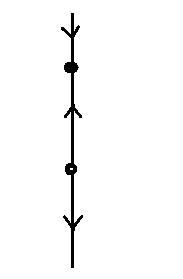
\includegraphics[width=\linewidth]{images/1.6-Phase1.png}
\end{image}%
\tcblower
\end{figureptx}%
For example, the phase line shows that as \(y\) is close to \(y=1\) from below, then the function keeps increasing, and thus must approach asymptotically to the equilibrium solution.%
\par
A sketch of some possible solutions looks like: \begin{figureptx}{Solution sketch for \(\frac{dy}{dt} = y(1-y)\)}{x:figure:fig-sketch1}{}%
\begin{image}{0.3}{0.4}{0.3}%
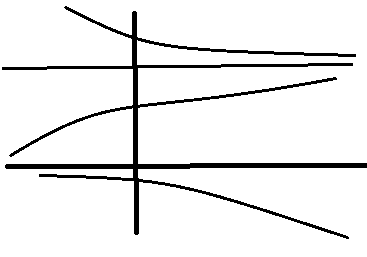
\includegraphics[width=\linewidth]{images/1.6-Sketch1.png}
\end{image}%
\tcblower
\end{figureptx}%
%
\par
From our first sketch we can always notice the following things about sketching curves:%
%
\begin{enumerate}
\item{}If \(f(y(0))=0\) then \(y(0)\) is an equilibirum solution and \(y(t)=y(0)\) for all \(t\).%
\item{}If \(f(y(0))>0\) then \(y(t)\) is \emph{increasing} for all \(t\) and either \(y(y)\to\infty\) as \(t\to\infty\) or \(y(t)\) tends to first equilibirum point \emph{larger} than \(y(0).\)%
\item{}If \(f(y(0))
\lt 0\) then then \(y(t)\) is \emph{decreasing} for all \(t\) and either \(y(y)\to-\infty\) as \(t\to\infty\) or \(y(t)\) tends to first equilibirum point \emph{smaller} than \(y(0).\)%
\end{enumerate}
\begin{example}{Curve Sketching.}{g:example:id403276}%
We let%
\begin{equation*}
\frac{dy}{dt}=(2-y)\sin y.
\end{equation*}
%
%
\begin{enumerate}
\item{}Find equilibrium points \(y=2\) and \(y=n\pi\) (so infinite amount)%
\item{}Plug points and get that the phase line is : \begin{image}{0.35}{0.3}{0.35}%
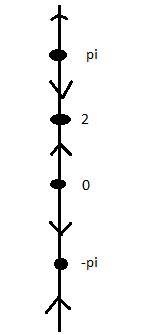
\includegraphics[width=\linewidth]{images/1.6-Phase2.png}
\end{image}%
%
\item{}Talk about what happens when things are getting close to the equilibrium solutions.%
\item{}Sketch curves: \begin{image}{0}{1}{0}%
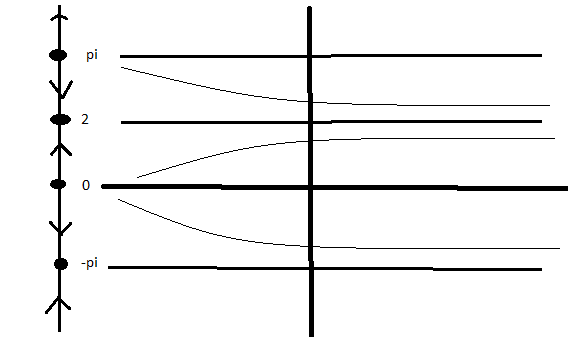
\includegraphics[width=\linewidth]{images/1.6-Sketch2.png}
\end{image}%
%
\end{enumerate}
\end{example}
\begin{example}{We don't know how quickly solutions increase\slash{}decrease with respect to time.}{g:example:id403322}%
Show that the graph \(\frac{dP}{dt}=(1-\frac{P}{20})^{3}(\frac{P}{5}-1)P^{7}\) has Phase line \(\begin{array}{c}
\vee\\
20\\
\wedge\\
5\\
\vee\\
0\\
\wedge
\end{array}\)%
\par
By plotting a graph of actual solutions, you'll see that solutions between \(y=5\) and \(y=20\), increase very rapidly. See the following slope field.%
\begin{sageinput}
t,y=var('t,y')
plot_slope_field((1 - y/20)^3 * (y/5 - 1) *y^7, (t,-5,5), (y,0, 20))
\end{sageinput}
\end{example}
\begin{example}{Not all solutions exist for all \(t\).}{g:example:id403370}%
Consider the equation \(\frac{dy}{dt}=(1+y)^{2}\).%
\par
The phase line is  \(\begin{array}{c}
\wedge\\
-1\\
\wedge
\end{array}\) Sketch a curve.%
\par
The Phase Line doesn't tell us if there could be any vertical assymptotes. (Phase LINE DOES NOT TELL US THIS INFO)%
\par
ACTUAL SOLUTION: \(y(t)=-1-\frac{1}{t+c}\). Note that there is an assymptote at \(t=c\).%
\par
If \(y(0)>-1\) then draw possible curve.%
\begin{sageinput}
t,y=var('t,y')
g = Graphics()
g+= plot_slope_field((1+y)^2, (t,-5,5),(y,-5,5))
g+= plot(-1-1/(t + 2), (t,-5,5), ymax = 5, ymin = -5)
g.show()
\end{sageinput}
\end{example}
\begin{example}{Cusps.}{g:example:id403421}%
Consider the equation \(\frac{dy}{dt}=\frac{1}{1-y}\).%
\par
The phase line would be: \begin{image}{0.35}{0.3}{0.35}%
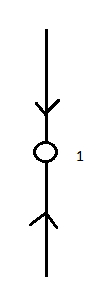
\includegraphics[width=\linewidth]{images/1.6-Phase3.png}
\end{image}%
 We drew a hole\slash{}circle for \(y=1\) since the derivative can't exit there. It turns out that for Phase Lines with holes, its solutions tend to have cusps. See the graph below.%
\begin{sageinput}
t,y=var('t,y')
g = Graphics()
g+= plot_slope_field(1/(1-y), (t, -5, 5), (y, -5, 5))
g+= plot(1 + sqrt(-2*t + 4), (t, -5, 2))
g+= plot(1 - sqrt(-2*t -2), (t, -5, -1), color="red")
g.show()
\end{sageinput}
\end{example}
\alert{Role of Equilibrium points:}%
\par
The solutions to autonomous equations either%
\begin{enumerate}
\item{}Tend to \(\pm\infty\)%
\item{}Tend to the equilibrium solutions.%
\item{}Stay consistently increasing\slash{}decreasing within equilibrium solutions.%
\end{enumerate}
%
\end{subsectionptx}
%
%
\typeout{************************************************}
\typeout{Subsection 2.7.3 Classification of Equilibrium Solutions}
\typeout{************************************************}
%
\begin{subsectionptx}{Classification of Equilibrium Solutions}{}{Classification of Equilibrium Solutions}{}{}{g:subsection:id403441}
Recall what \terminology{asymptotic} means: say that \(f\) is asymptotic to the line \(y = c\) if%
\begin{equation*}
\lim_{t \to \infty} f(t) = c.
\end{equation*}
%
\par
We can classify the equilibrium solutions to an autonomous equation by looking at the behavior of ``nearby'' solutions. Solutions fall into one of three categories.%
%
\begin{enumerate}
\item{}\alert{Asymptotically stable (sink)}%
%
\begin{enumerate}
\item{}\(y_{0}\) is an \terminology{asymptotically stable} equilibrium if any solution with initial condition sufficiently close to \(y_{0}\) is asymptotic to \(y_{0}\) as \(t\) increases.%
\item{}Phase Line looks like this:  \(\begin{array}{c}
\vee\\
y_{0}\\
\wedge
\end{array}\)%
\item{}Graph looks like: (reminds you that it is falling into something)%
\item{}In a graph of \(f(y)\) vs. \(y\), we have \(f^{\prime}(y_{0}) \lt 0\).%
\end{enumerate}
\item{}\alert{Asymptotically unstable (source):}%
%
\begin{enumerate}
\item{}\(y_{0}\) is an \terminology{asymptotically unstable} equilibrium if any solution with initial condition sufficiently close to \(y_{0}\) tends torward \(y_{0}\) as \(t\) decreases.%
\item{}The phase line looks like this:  \(\begin{array}{c}
\wedge\\
y_{0}\\
\vee
\end{array}\)%
\item{}Graph looks like: ( reminds you that it is coming from one place)%
\item{}In \(f(y)\) vs. \(y\) graph, we have \(f^{\prime}(y_{0})>0\).%
\end{enumerate}
\item{}\alert{Semistable(node):}%
%
\begin{enumerate}
\item{}\(y_{0}\) is an \alert{asymptotically semistable} equilibrium if it doesn't fit the category of a sink or source \textbackslash{}item Phase Line looks like this:  \(\begin{array}{c}
\wedge\\
y_{0}\\
\wedge
\end{array}\)or  \(\begin{array}{c}
\vee\\
y_{0}\\
\vee
\end{array}\)%
\item{}Graph looks like:%
\end{enumerate}
\end{enumerate}
\begin{example}{Drawing solution from the \(f(y)\) vs. \(y\) graph).}{g:example:id403698}%
Consider the equation \(\frac{dy}{dt}=y^{2}+y-6=(y+3)(y-2)\).%
\par
The phase line is \(\begin{array}{c}
\wedge\\
2\\
\vee\\
-3\\
\wedge
\end{array}\)%
\par
How can these be classified?%
\par
\(y_{0}=2\) is assymptotically unstable while \(y_{0}=-3\) is assymptotically stable.%
\end{example}
\begin{example}{(Using \(f(y)\)).}{g:example:id403877}%
We can figure out classification directly from the graph of \(f(y)\). \begin{image}{0}{1}{0}%
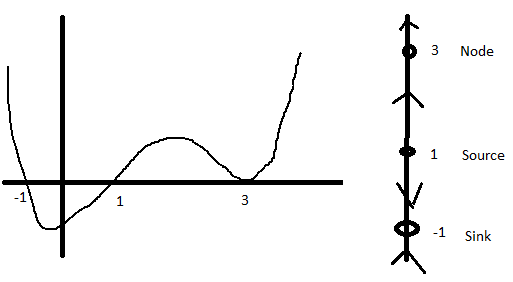
\includegraphics[width=\linewidth]{images/1.6-Classif-1.png}
\end{image}%
 Here, node means semistable, sink means stable, and source means unstable.%
\end{example}
\begin{example}{}{g:example:id403997}%
Suppose we only know the graph of \(f(y)\) not the actual formula. \begin{image}{0}{1}{0}%
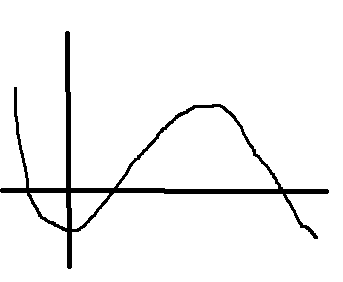
\includegraphics[width=\linewidth]{images/1.6-f(y).png}
\end{image}%
 Then draw phase line : \(\begin{array}{c}
\vee\\
c\\
\wedge\\
b\\
\vee\\
a\\
\wedge
\end{array}\) Now sketch some solution curves.%
%
\end{example}
\end{subsectionptx}
\end{sectionptx}
%
%
\typeout{************************************************}
\typeout{Section 2.8 Exact equations}
\typeout{************************************************}
%
\begin{sectionptx}{Exact equations}{}{Exact equations}{}{}{x:section:ch2-8}
\begin{introduction}{}%
This section introduces a family of equations that arise naturally in physical contexts. For example, suppose that we had a detailed temperature map of a hot metal sheet. Can we predict how the heat will flow? The answer to this question is provided by the gradient, studied in multi-variable calculus. But what about the opposite scenario? Given a heat flow map, can we reconstruct the original temperature distribution? To answer this question, we'll consider what are known as \terminology{exact equations}. First, we recall some multivariable calculus.%
\end{introduction}%
%
%
\typeout{************************************************}
\typeout{Subsection 2.8.1 Partial derivatives and the gradient}
\typeout{************************************************}
%
\begin{subsectionptx}{Partial derivatives and the gradient}{}{Partial derivatives and the gradient}{}{}{g:subsection:id404094}
Suppose that \(z = f(x,y)\) is a function of two independent variables. Just as in one variable, we want to understand how the graph of \(f\) changes at a point, but now we have lots of different directions to look at. To compute the rate of change in the \(x\) and \(y\) directions, we can use the \terminology{partial derivative} in those directions. When we take a partial derivative with respect to a variable, we treat all other variables as constant so that we're isolating our view to change in that specific direction.%
\begin{definition}{}{g:definition:id404128}%
Let \(z = f(x,y)\). The partial derivative of \(f\) with respect to \(x\) is%
\begin{equation*}
\frac{\partial f}{\partial x} = \lim_{h \to 0} \frac{f(x + h, y) - f(x,y)}{h}.
\end{equation*}
The partial derivative of \(f\) with respect to \(y\) is%
\begin{equation*}
\frac{\partial f}{\partial y} = \lim_{h\to 0}\frac{f(x, y+h) - f(x,y)}{h}.
\end{equation*}
%
\end{definition}
In practice, we can use the single variable differentiation rules, treating the other variable like it is a fixed number. For example,%
\begin{equation*}
\frac{\partial}{\partial x} x^2 + x \cos y + y^2 = 2x + \cos y + 0.
\end{equation*}
%
\par
Frequently, when given a function \(z = f(x,y)\), we wish to know the direction of greatest slope or rate of change. For example, if \(z = f(x,y)\) represents the height of a mountain, the direction that water flows downhill will be in the direction of sleepest descent. We can use the partial derivatives to define a \terminology{vector field} that at each point \((x,y)\) gives the direction of greatest slope of the graph of \(f\).%
\begin{definition}{}{g:definition:id404203}%
The \terminology{gradient} of \(z = f(x,y)\) is the vector-valued function%
\begin{equation*}
\nabla f = \langle \frac{\partial f}{\partial x}, \frac{\partial f}{\partial y}\rangle.
\end{equation*}
This is written shorthand as \(\nabla f = \langle f_x, f_y\rangle\).%
\end{definition}
You should think of the gradient in this context as a slope field - at every point in the \(x-y\) plane, the gradient attaches a vector that indicates the direction of greatest slope.%
\par
If we think of \(z = f(x,y)\) as a voltage map or a temperature map or a height map, a standard visualization is to use curves to represent points that have equal heights. Such curves are called \terminology{isotherms} or \terminology{equipotential lines} or altitude lines.%
\begin{example}{Equipotentials and surfaces.}{g:example:id404303}%
Let \(f(x, y) = -x^2 + 3y - y^2\). The following code will plot some equipotentials of \(f\). In particular, we will plot the curves corresponding to \(z = 0, 1, 2\).%
\begin{sageinput}
x,y = var('x,y')
g = Graphics()
g+= implicit_plot(-x^2  + 3*y - y^2, (x, -2,2), (y, 0,3), color = "red" )
g+=implicit_plot(-x^2  + 3*y - y^2 - 1, (x, -2,2), (y, 0,3), color="yellow" )
g+= implicit_plot(-x^2  + 3*y - y^2-2, (x, -2,2), (y, 0,3), color="green" )
g.show()
\end{sageinput}
 Now compare to the surface itself: \begin{sageinput}
var('x y z')
f(x, y) = -x^2  + 3*y - y^2
P = implicit_plot3d(f-z, (x ,-1, 3), (y, 0, 3), (z, -2, 3))
Q = plot3d(0, (-1,3), (0,3), color="red", opacity=".4")
R = plot3d(1, (-1,3), (0,3), color="yellow", opacity = ".4")
S = plot3d(2, (-1,3), (0,3), color ="green", opacity = ".4")
P + Q +R +S
\end{sageinput}
\end{example}
\begin{example}{Relationship between equipotentials and gradients.}{g:example:id404327}%
One of the most important geometric facts about the relationship between the \terminology{potential function} \(f\) and the gradient field \(\nabla f\) is that \emph{equipotentials are perpendicular to gradients.} Using our previous example:%
\begin{sageinput}
x,y = var('x,y')
g = Graphics()
g+= implicit_plot(-x^2  + 3*y - y^2, (x, -2,2), (y, 0,3), color = "red" )
g+=implicit_plot(-x^2  + 3*y - y^2 - 1, (x, -2,2), (y, 0,3), color="yellow" )
g+= implicit_plot(-x^2  + 3*y - y^2-2, (x, -2,2), (y, 0,3), color="green" )
g+= plot_vector_field((-2*x, 3 - 2*y), (-2,2), (0,3))
g.show()
\end{sageinput}
\end{example}
In summary, given a \terminology{potential function} \(z = f(x,y)\),%
\begin{enumerate}
\item{}We can find the equipotential lines (lines of constant height)%
\begin{equation*}
C = f(x,y);
\end{equation*}
%
\item{}we can find the gradient field%
\begin{equation*}
\nabla f = \langle f_x, f_y \rangle;
\end{equation*}
%
\item{}and we know that at a given point, the equipotential and the gradient line are perpendicular.%
\end{enumerate}
%
\end{subsectionptx}
%
%
\typeout{************************************************}
\typeout{Subsection 2.8.2 From gradient field to potential function}
\typeout{************************************************}
%
\begin{subsectionptx}{From gradient field to potential function}{}{From gradient field to potential function}{}{}{g:subsection:id404400}
How do we know when we can go the other direction? That is, as we asked at the top of the section, when given a vector field \(F(x,y) = (M(x,y), N(x,y))\), how can we recover a potential function \(f\)? Essentially, this is asking us to find a function so that \(\nabla f = F\) (the ``antiderivative of \(F\) is \(f\)''). Like integration problems, this may not always exist.%
\begin{definition}{}{g:definition:id404431}%
A vector field \(F\) is called \terminology{conservative} if there exists a potential function \(f\) so that \(\nabla f = F\).%
\end{definition}
One marker of nice functions in two variables is the conclusion of \terminology{Clairaut's theorem}, which states that the \terminology{mixed partial derivatives} of \(f\) are equal - that is, for a nice \(f\),%
\begin{equation*}
\frac{\partial^2 f}{\partial x \partial y} = \frac{\partial^2 f}{\partial y \partial x}.
\end{equation*}
Suppose for the moment that a vector field%
\begin{equation*}
F = \langle M, N \rangle = \nabla f = \langle f_x, f_y \rangle
\end{equation*}
and that the derivatives \(f_{xx}, f_{yy}, f_{xy}, f_{yx}\) all exist and are continuous. Clairaut's theorem will force%
\begin{equation*}
\frac{\partial M}{\partial y} = f_{xy} = f_{yx} = \frac{\partial N}{\partial x}\text{.}
\end{equation*}
It turns out to be the case that this condition, \(M_y = N_x\), is not only necessary but sufficient on nice enough domains like rectangles.%
\begin{theorem}{}{}{g:theorem:id404532}%
Let \(F = \langle M(x,y), N(x,y) \rangle\) be a vector field so that the partial derivatives of \(M\) and \(N\) exist and are continuous on a rectangle \(a \leq x \leq b, c \leq y \leq d\). Then there exists a potential function \(f\) so that \(\nabla f = F\) if%
\begin{equation*}
M_y = N_x.
\end{equation*}
%
\end{theorem}
\end{subsectionptx}
%
%
\typeout{************************************************}
\typeout{Subsection 2.8.3 Differential equations and equipotentials}
\typeout{************************************************}
%
\begin{subsectionptx}{Differential equations and equipotentials}{}{Differential equations and equipotentials}{}{}{g:subsection:id404573}
The \terminology{total derivative} of a function \(z = f(x,y)\) is given by the expression%
\begin{equation*}
df = f_x \, dx + f_y \, dy.
\end{equation*}
Notice that the functions that appear as components in \(df\) are the components of the gradient \(\nabla f\). If we were given the equation of an equipotential for \(f\), say%
\begin{equation*}
f(x, y) = C,
\end{equation*}
then the total derivative of the equation is%
\begin{align*}
\amp df = dC \\
\Rightarrow \amp f_x \, dx + f_y \, dy = 0\\
\Rightarrow \amp M \, dx + N \, dy = 0.
\end{align*}
If we have further that \(f\) has continuous second partial derivatives on a rectangle \(a \leq x \leq b, c \leq y \leq d\), then Clairaut's theorem gives%
\begin{equation*}
M_y = f_{xy} = f_{yx} = N_x.
\end{equation*}
%
\par
The upshot of all of this is that we can view an equation of the form%
\begin{equation*}
M \, dx + N \, dy = 0
\end{equation*}
as a differential equation that seeks to find the equipotentials \(f(x,y) = C\) for some unknown function \(f\) with \(\nabla f = \langle M, N \rangle\).%
\end{subsectionptx}
%
%
\typeout{************************************************}
\typeout{Subsection 2.8.4 Exact equations}
\typeout{************************************************}
%
\begin{subsectionptx}{Exact equations}{}{Exact equations}{}{}{g:subsection:id404658}
Consider an equation \(M(x,y)dx+N(x,y)dy=0.\) We say this equation is \terminology{exact} if \(\frac{\partial M}{\partial y}=\frac{\partial N}{\partial x};\) that is, as discussed in the previous section, the equation represents a differential equation that seeks to find equipotentials of a function \(f\) so that \(\nabla f = \langle M, N \rangle\).%
\begin{example}{}{g:example:id404696}%
Suppose \(\frac{dy}{dx}=\frac{-2x-y^{2}}{2xy}.\) We can rewrite this as \(\left(2x+y^{2}\right)dx+2xydy=0\) then \(M=2x+y^{2}\) and \(N=2xy\). Computing the partial derivatives,%
\begin{align*}
M_{y} \amp =2y\\
N_{x} \amp =2y
\end{align*}
are \(M_{y}=N_{x}\). Thus this equation is exact.\end{example}
\begin{theorem}{}{}{g:theorem:id404735}%
If \(M,N,M_{y},N_{x}\) are all continuous on a rectangle \([a,b]\times[c,d]\) and%
\begin{equation*}
M\,dx+N\,dy=0
\end{equation*}
is exact then there exists a function \(\psi\) such that%
\begin{equation*}
\psi_{x}(x,y)=M(x,y)\text{ and }\psi_{y}(x,y)=N(x,y)
\end{equation*}
and such that \(\psi(x,y)=C\) gives an implicit solution to the ODE.%
\end{theorem}
\begin{proof}{}{g:proof:id404777}
If \(\psi\) satisfies \(\psi_{x}=M\) and \(\psi_{y}=N\) such that \(\psi(x,y)=C\) then \(\psi\) defines a function \(y=\phi(x)\) implicitly. Then we show \(\phi(x)\) solves the ODE. Note that \(0=M(x,y)+N(x,y)y^{\prime}=\frac{\partial\psi}{\partial x}+\frac{\partial\psi}{\partial y}\frac{dy}{dx}=\frac{d}{dx}\left(\psi\left(x,\phi(x)\right)\right)\) by the multivariable chain rule. Thus if we integrate both sides%
\begin{align*}
\amp 0 =\frac{d}{dx}\left(\psi\left(x,\phi(x)\right)\right) \\
\iff\amp \int0dx=\int\frac{d}{dx}\left(\psi\left(x,\phi(x)\right)\right)dx\\
\iff \amp c=\psi\left(x,\phi(x)\right),
\end{align*}
as needed.\end{proof}
\alert{Solving exact equations:} If \(Mdx+Ndy=0\) is exact then%
\begin{align*}
\amp \psi_{x}=M(x,y) \amp \implies \amp \psi=\int M(x,y)dx+h(y)\\
\amp \amp \amp \Downarrow\\
\amp \psi_{y}=N(x,y) \amp \amp \psi_{y}=\frac{\partial}{\partial y}\left(\int M(x,y)dx\right)+h^{\prime}(y)
\end{align*}
and then solve for \(h(y)\).%
\par
\alert{Another way:} One may also solve it by starting with the second equation:%
\begin{align*}
\amp \psi_{x}=M(x,y) \amp \amp \psi_{x}=\frac{\partial}{\partial x}\left(\int N(x,y)dx\right)+g^{\prime}(x)\\
\amp \amp \amp \Uparrow\\
\amp\psi_{y}=N(x,y)\implies \amp \amp\psi=\int N(x,y)dy+g(x).
\end{align*}
%
\begin{example}{}{g:example:id505598}%
We know \(\left(2x+y^{2}\right)dx+2xydy=0\) is exact.%
\begin{enumerate}
\item{}Show it's exact(done earlier) and follow the arrows until you close the diagram:%
\begin{align*}
\text{Start here:} \amp \psi_{x}=2x+y^{2} \amp \implies \amp \psi=\int\left(2x+y^{2}\right)dx+h(y)\\
\amp  \amp  \amp \boldsymbol{\psi=x^{2}+y^{2}x+h(y)}\\
\amp  \amp  \amp \Downarrow\\
\amp \psi_{y}=2xy \amp \Longleftarrow \amp \psi_{y}=2xy+h^{\prime}(y)
\end{align*}
%
\item{}Solve for \(h(y)\) by noting that since%
\begin{align*}
2xy=2xy+h^{\prime}(y)\implies \amp h^{\prime}(y)=0\\
\implies \amp h(y)=C.
\end{align*}
%
\item{}Put it all together and get \(\psi(x,y)=x^{2}+y^{2}x+C\) and hence the \emph{implicit solution} is \(x^{2}+y^{2}x=C.\)%
\end{enumerate}
%
\end{example}
\begin{example}{}{g:example:id505800}%
Solve \(\left(y\cos x+2xe^{y}\right)+\left(\sin x+x^{2}e^{y}-y^{2}\right)y^{\prime}=0.\)%
\par
%
\begin{enumerate}
\item{}To show it's exact note that \(\left(y\cos x+2xe^{y}\right)dx+\left(\sin x+x^{2}e^{y}-y^{2}\right)dy=0,\) and not hard to see that%
\begin{align*}
M_{y} \amp =\cos x+2xe^{y}\\
N_{x} \amp =\cos x+2xe^{y}
\end{align*}
and they are equal, thus this ODE is exact. Follow the arrows until close the diagram:%
\begin{align*}
\text{Start here:} \amp \psi_{x}=y\cos x+2xe^{y} \amp \implies \amp \psi=\int\left(y\cos x+2xe^{y}\right)dx+h(y)\\
\amp  \amp  \amp \boldsymbol{\psi=y\sin x+x^{2}e^{y}+h(y)}\\
\amp  \amp  \amp \Downarrow\\
\amp \psi_{y}=\sin x+x^{2}e^{y}-y^{2} \amp \Longleftarrow \amp \psi_{y}=\sin x+x^{2}e^{y}+h^{\prime}(y)
\end{align*}
%
\item{}Solve for \(h(y)\) by noting that since%
\begin{align*}
\sin x+x^{2}e^{y}-y^{2}=\sin x+x^{2}e^{y}+h^{\prime}(y)\implies \amp h^{\prime}(y)=-y^{2}\\
\implies \amp h(y)=-\frac{y^{3}}{3}
\end{align*}
%
\item{}Put it all together and get \(\psi(x,y)=y\sin x+x^{2}e^{y}-y\) and hence the \emph{implicit solution} is \(y\sin x+x^{2}e^{y}-\frac{y^{3}}{3}=C.\)%
\end{enumerate}
%
\begin{sageinput}
var('x,y')
P = plot_vector_field((y*cos(x) + 2*x*e^y, sin(x) + x^2*e^y - y^2), (-3,3),(-3,3))
Q = implicit_plot(y *sin(x) + x^2*e^y - y^3/3 - 5,(-3,3),(-3,3), color="red")
R = implicit_plot(y *sin(x) + x^2*e^y - y^3/3 - 3,(-3,3),(-3,3), color ="orange")
S = implicit_plot(y *sin(x) + x^2*e^y - y^3/3,(-3,3),(-3,3), color ="blue")
P + Q +R +S
\end{sageinput}
\end{example}
\begin{example}{}{g:example:id506044}%
Find the value of \(b\) for which the given equation is exact, and then solve it using that \(b\): \(\left(xy^{2}+bx^{2}y\right)dx+\left(x+y\right)x^{2}dy\)%
\begin{enumerate}
\item{}If this equation is exact then \(M_{y}=N_{x}\),%
\begin{align*}
M_{y} \amp =2xy+bx^{2}\\
N_{x} \amp =3x^{2}+2yx
\end{align*}
and are only equal when \(b=3\). Follow the arrows until close the diagram:%
\begin{align*}
\text{Start here:} \amp \psi_{x}=xy^{2}+3x^{2}y \amp \implies \amp \psi=\int\left(xy^{2}+3x^{2}y\right)dx+h(y)\\
\amp  \amp  \amp \boldsymbol{\psi=\frac{1}{2}x^{2}y^{2}+x^{3}y+h(y)}\\
\amp  \amp  \amp \Downarrow\\
\amp \psi_{y}=x^{3}+x^{2}y \amp \Longleftarrow \amp \psi_{y}=x^{2}y+x^{3}+h^{\prime}(y)
\end{align*}
%
\item{}Solve for \(h(y)\) by noting that since%
\begin{align*}
x^{3}+x^{2}y=x^{2}y+x^{3}+h^{\prime}(y)\implies \amp h^{\prime}(y)=0\\
\implies \amp h(y)=C
\end{align*}
%
\item{}Put it all together and get \(\psi(x,y)=\frac{1}{2}x^{2}y^{2}+x^{3}y+C\) and hence the \emph{implicit solution} is \(\frac{1}{2}x^{2}y^{2}+x^{3}y=C.\)%
\end{enumerate}
\end{example}
\begin{example}{}{g:example:id506288}%
Solve \(\left(x\cos x+e^{y}\right)dx+xe^{y}dy\)%
%
\begin{enumerate}
\item{}If this equation is exact then \(M_{y}=N_{x}\), and%
\begin{align*}
M_{y} \amp =e^{y}\\
N_{x} \amp =e^{y}
\end{align*}
Now note that it is actually easier to integrate \(N\) with respect to \(y\): Thus we can start the diagram in the other direction%
\begin{align*}
\amp \psi_{x}=x\cos x+e^{y} \amp \Longleftarrow \amp =\psi_{x}=e^{y}+g^{\prime}(x)\\
\amp  \amp  \amp \boldsymbol{\psi=xe^{y}+g(x)}\\
\amp  \amp  \amp \Uparrow\\
\text{Start here:} \amp \psi_{y}=xe^{y} \amp \implies \amp \psi_{y}=\int\left(xe^{y}\right)dy+g(x)
\end{align*}
%
\item{}Solve for \(g(x)\) by noting that since%
\begin{align*}
x\cos x+e^{y}=e^{y}+g^{\prime}(x)\implies \amp g^{\prime}(x)=x\cos x
\end{align*}
but at the end of the day we can't avoid the harder integration, as we still need to integration by parts to \(g(x)=x\sin x+\cos x\)%
\item{}Put it all together and get \(\psi(x,y)=xe^{y}+x\sin x+\cos x\) and hence the \emph{implicit solution} is \(xe^{y}+x\sin x+\cos x=C.\)%
\end{enumerate}
\begin{sageinput}
var('x,y')
P = plot_vector_field((x*cos(x) + e^y, x*e^y), (-3,3),(0,5))
Q = implicit_plot(x*e^y + x*sin(x) + cos(x) - 120,(-3,3),(0,5), color="red")
R = implicit_plot(x*e^y + x*sin(x) + cos(x) - 50,(-3,3),(0,5), color ="orange")
S = implicit_plot(x*e^y + x*sin(x) + cos(x) - 10,(-3,3),(0,5), color ="blue")
P + Q +R +S
\end{sageinput}
\end{example}
\end{subsectionptx}
\end{sectionptx}
%
%
\typeout{************************************************}
\typeout{Section 2.9 Euler's method}
\typeout{************************************************}
%
\begin{sectionptx}{Euler's method}{}{Euler's method}{}{}{x:section:ch2-9}
\begin{introduction}{}%
In practice, many if not most differential equations do not have explicit solutions. If an equation does happen to fall into a form that we have a solution method for, there is no guarantee that we can integrate the result. Thus, it is important to have approaches that can sketch curves and approximate solutions in the absence of explicit formulas.%
\par
One of the most straightforward approaches to first order equations of the form%
\begin{equation*}
\frac{dy}{dt} = f(t,y)
\end{equation*}
is \terminology{Euler's method}, which approximates a solution to an initial value problem with small pieces of tangent line.%
\par
Suppose we are given an initial value problem%
\begin{equation*}
\frac{dy}{dt}=f(t,y)\qquad y(t_{0})=y_{0}.
\end{equation*}
%
%
\begin{itemize}[label=\textbullet]
\item{}Let \(h=\) step size. These are our \(t-\)axis increments.%
\item{}Let \(t_{0}=\) our starting point. Then our next point will be \(t_{1}=t_{0}+h\), then \(t_{2}=t_{1}+h\). Notice that this means%
\begin{equation*}
t_{k+1} - t_k = h.
\end{equation*}
%
\end{itemize}
For example suppose \(t_{0}=1\) and \(h=.5\), then \(t_{0}=1,t_{1}=1.5,t_{2}=2,\dots\). So how do we find the explicit values for \(y_{k}\) other than just guessing?%
\begin{observation}{}{g:observation:id506991}%
For small step size \(h\), the slope of the tangent line at \((t_0, y_0)\) is a reasonable approximation for the secant line connecting \((t_0, y(t_0))\) to the point \((t_1), y(t_1)\). That is,%
\begin{equation*}
\frac{y(t_{k+1}) - y(t_k)}{t_{k+1} - t_k} = \frac{y(t_{k+1}) - y(t_k)}{h} \approx f(t_k, y(t_k)).
\end{equation*}
\end{observation}
Let \(y_0 = y(t_0)\). Now, denote by \(y_1\) the \emph{approximation} of \(y(t_1)\) given by%
\begin{equation*}
y(t_1) \approx y_1 := y_0 + f(t_0, y_0) h.
\end{equation*}
Iteration of this idea to produce a larger approximate graph of a solution is the key idea of Euler's method.%
\end{introduction}%
%
%
\typeout{************************************************}
\typeout{Subsection 2.9.1 Euler's method}
\typeout{************************************************}
%
\begin{subsectionptx}{Euler's method}{}{Euler's method}{}{}{g:subsection:id507199}
\begin{definition}{}{g:definition:id507198}%
Given an initial condition \(y(t_{0})=y_{0}\) and step size \(h\), compute \(\left(t_{k+1},y_{k+1}\right)\) from the preceding point \((t_{k},y_{k})\) as follows:%
\begin{align*}
t_{k+1} \amp = \amp t_{k}+h\\
y_{k+1} \amp = \amp y_{k}+f\left(t_{k},y_{k}\right)h.
\end{align*}
%
\end{definition}
 One can check their work using the following application, which computes all the points for Euler's Method: \href{https://davidmathlogic.com/euler/}{Euler's Method Applet}\begin{example}{}{g:example:id507343}%
Suppose we have the autonomous equation%
\begin{align*}
\frac{dy}{dt}=2y-1 \amp  \amp ,y(0)=1,
\end{align*}
with \(h=0.1\) and \(0\leq t\leq1\).%
%
\begin{enumerate}
\item{}Our first point is \((t_{0},y_{0})=\left(0,1\right)\).%
\item{}We can compute the formula for this and get \(t_{k+1}=t_{k}+.1\) and notice that \(f\left(t,y\right)=2y-1\).%
\begin{equation*}
y_{k+1}=y_{k}+f\left(t_{k},y_{k}\right)h=y_{k}+\left(2y_{k}-1\right)(.1).
\end{equation*}
%
\item{}Make a table:%
\begin{equation*}
\begin{array}{|c|c|c|c|}
\hline
k \amp t_{k} \amp y_{k}=y_{k-1}+f\left(t_{k-1},y_{k-1}\right)h \amp f\left(t_{k},y_{k}\right)=2y_{k}-1\\
\hline
\hline
0 \amp 0 \amp 1 \amp 1\\
\hline
1 \amp 0.1 \amp y_{1}=1+1\cdot(.1)=\mathbf{1.1} \amp f\left(t_{1},y_{1}\right)=2(1.1)-1=\mathbf{1.20}\\
\hline
2 \amp 0.2 \amp y_{2}=1.1+(1.20)\cdot(.1)=\mathbf{1.22} \amp f\left(t_{2},y_{2}\right)=2(1.22)-1=\mathbf{1.44}\\
\hline
3 \amp 0.3 \amp y_{3}=1.22+(1.20)\cdot(.1)=\mathbf{1.364} \amp f\left(t_{3},y_{3}\right)=2(1.22)-1=\mathbf{1.73}\\
\hline
4 \amp 0.4 \amp 1.537 \amp 2.07\\
\hline
\amp .5 \amp 1.744 \amp 2.49\\
\hline
\amp .6 \amp 1.993 \amp 2.98\\
\hline
\amp .7 \amp 2.292 \amp 3.58\\
\hline
\amp .8 \amp 2.65 \amp 4.3\\
\hline
\amp 0.9 \amp 3.080 \amp 5.16\\
\hline
\amp 1.0 \amp 3.596 \amp 3.596\\
\hline
\end{array}
\end{equation*}
%
\end{enumerate}
Notice that actual value is \(y(1)=\frac{e^{2}+1}{2}=4.195\) and our approximation is \(y(1)\approx3.596\), which is a little short, but it makes sense all the slopes are always below the graph.%
\end{example}
\begin{example}{}{g:example:id507486}%
Our previous example didn't have any \(t\)s to plug in. So suppose we have%
\begin{equation*}
\frac{dy}{dt}=-2ty^{2},\quad y(0)=1,\quad h=\frac{1}{2}
\end{equation*}
%
%
\begin{enumerate}
\item{}Our first point is \((t_{0},y_{0})=\left(0,1\right)\).%
\item{}We can compute the formula for this and get \(t_{k+1}=t_{k}+.5\) and notice that \(f\left(t,y\right)=-2ty^{2}\).%
\begin{equation*}
y_{k+1}=y_{k}+f\left(t_{k},y_{k}\right)h=y_{k}+\left(-2t_{k}y_{k}^{2}\right)(\frac{1}{2}).
\end{equation*}
%
\item{}Make a table:%
\begin{equation*}
\begin{array}{|c|c|c|c|}
\hline
k \amp t_{k} \amp y_{k}=y_{k-1}+f\left(t_{k-1},y_{k-1}\right)h \amp f\left(t_{k},y_{k}\right)=-2t_{k}y_{k}^{2}\\
\hline
\hline
0 \amp 0 \amp 1 \amp 0\\
\hline
1 \amp \frac{1}{2} \amp y_{1}=1+0\cdot(\frac{1}{2})=\mathbf{1} \amp f\left(t_{1},y_{1}\right)=-2\frac{1}{2}1^{1}=\mathbf{-1}\\
\hline
2 \amp 1 \amp y_{2}=1+(-1)\cdot(\frac{1}{2})=\mathbf{\frac{1}{2}} \amp f\left(t_{2},y_{2}\right)=-2(1)(\frac{1}{2})^{2}=\mathbf{-\frac{1}{2}}\\
\hline
3 \amp 1.5=\frac{3}{2} \amp y_{3}=\frac{1}{2}+(-\frac{1}{2})\cdot(\frac{1}{2})=\frac{1}{4} \amp f\left(t_{3},y_{3}\right)=-2(\frac{3}{2})(\frac{1}{4})^{2}=\mathbf{-\frac{3}{16}}\\
\hline
4 \amp 2 \amp \frac{1}{4}+\left(-\frac{3}{16}\right)\cdot\left(\frac{1}{2}\right)=.15625 \amp \\
\hline
\end{array}
\end{equation*}
%
\end{enumerate}
A plot of our approximate solution is given below:%
\begin{image}{0}{1}{0}%
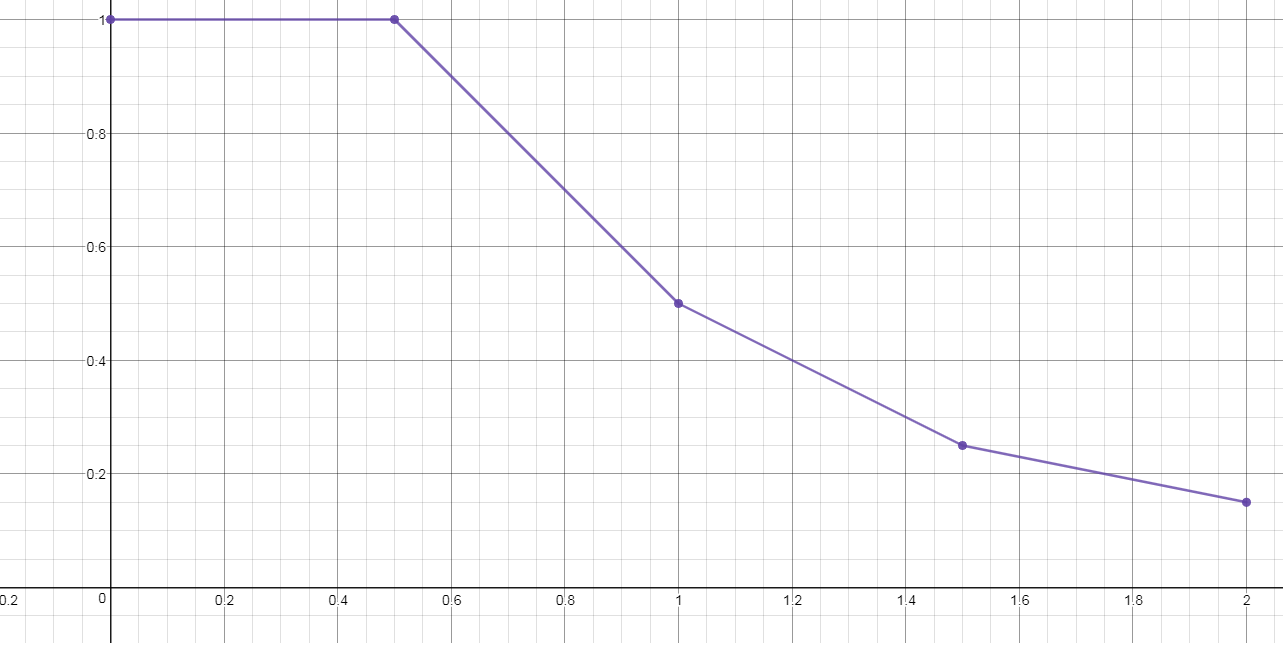
\includegraphics[width=\linewidth]{images/1.4-1.png}
\end{image}%
In code, this might look like%
\begin{sageinput}
var('t,y')
f(t, y) = -2*t*y^2
t0 = 0
y0 = 1
A = plot_slope_field(f, (0,3), (-1,3))

#approximate solution by Euler's method
h = .5
time = [t0 + n*h for n in range(5)]
yk = [y0]
def ynext(n):
    return yk[n-1] + f(time[n-1], yk[n-1])*h
for i in range(1,5):
    yk.append(ynext(i))
L = [[time[i], yk[i]] for i in range(5)]
B = line(L)

#actual solution
g(t) = 1/(t^2 + 1)
C = plot(g, (0,2), color = "red")
A + B + C
\end{sageinput}
\end{example}
\end{subsectionptx}
\end{sectionptx}
\end{chapterptx}
%
%
\typeout{************************************************}
\typeout{Chapter 3 Second Order Linear Equations}
\typeout{************************************************}
%
\begin{chapterptx}{Second Order Linear Equations}{}{Second Order Linear Equations}{}{}{x:chapter:ch3}
%
%
\typeout{************************************************}
\typeout{Section 3.1 Motivation - mass-spring systems.}
\typeout{************************************************}
%
\begin{sectionptx}{Motivation - mass-spring systems.}{}{Motivation - mass-spring systems.}{}{}{x:section:ch3-1}
\begin{introduction}{}%
This chapter is concerned with \terminology{second order differential equations}, and in particular those with \terminology{constant coefficients}. That is, we're going to be spending quite a bit of time thinking about equations of the form%
\begin{equation*}
a y'' + b y' + c y = 0
\end{equation*}
and%
\begin{equation*}
a y'' + b y' + c y = f(t).
\end{equation*}
At first glance, these equations seem artificially simple in structure. However, some of the most useful differential equations in the physical sciences and mathematics have this form, which motivates our close attention to second order linear equations with constant coefficients.%
\end{introduction}%
%
%
\typeout{************************************************}
\typeout{Subsection 3.1.1 Undamped mass-spring systems}
\typeout{************************************************}
%
\begin{subsectionptx}{Undamped mass-spring systems}{}{Undamped mass-spring systems}{}{}{g:subsection:id505534}
\begin{image}{0}{1}{0}%
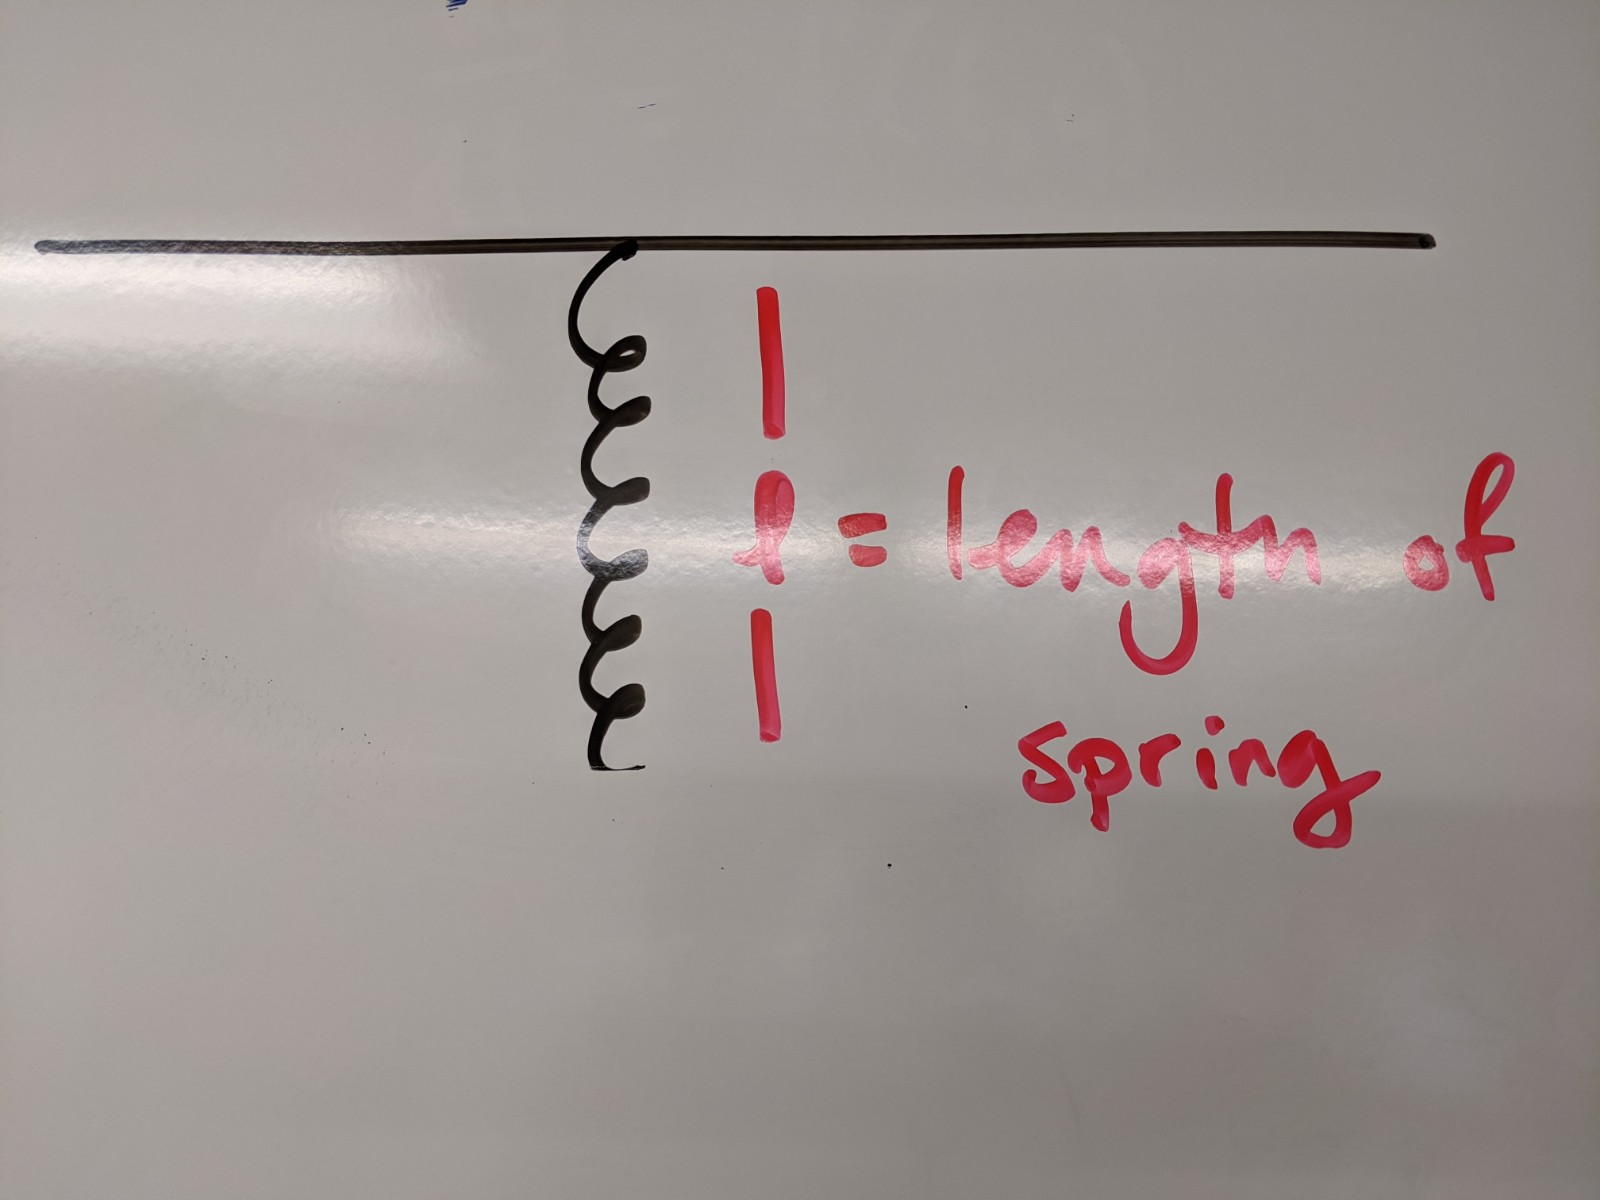
\includegraphics[width=\linewidth]{images/spring_no_mass.jpg}
\end{image}%
\begin{image}{0}{1}{0}%
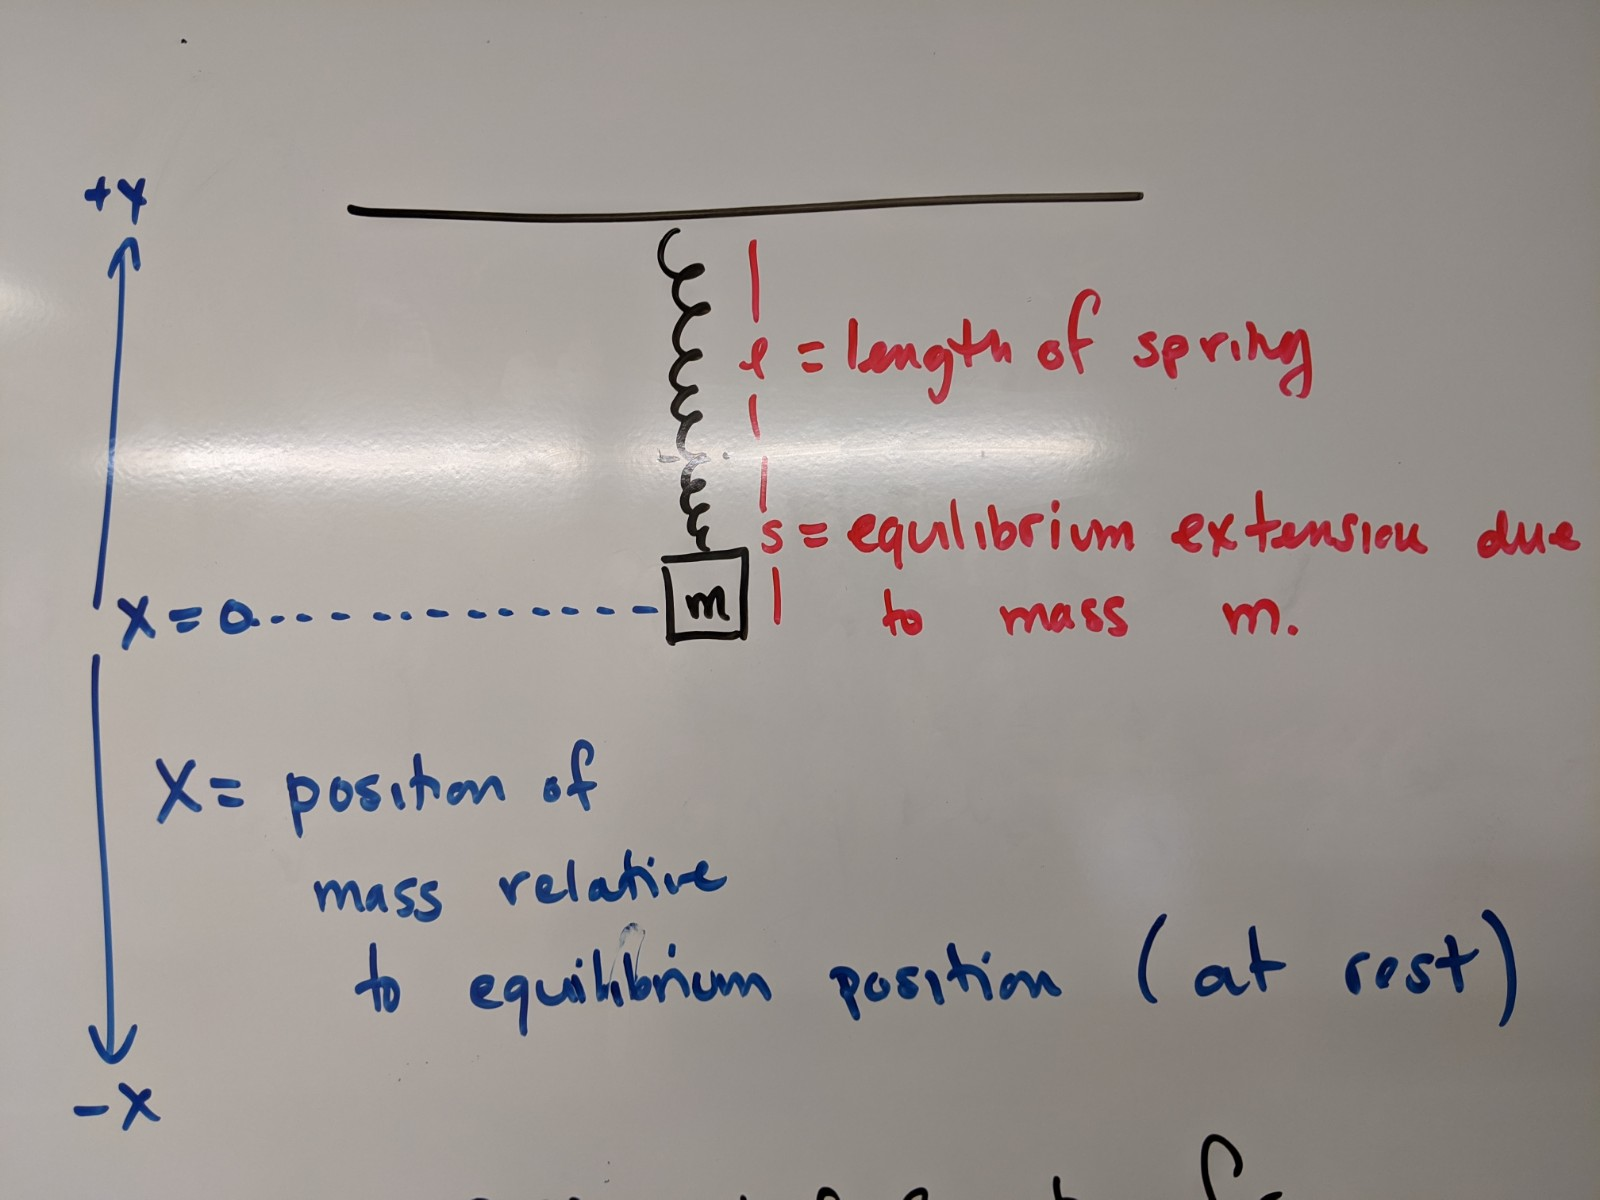
\includegraphics[width=\linewidth]{images/spring_eq.jpg}
\end{image}%
\begin{image}{0}{1}{0}%
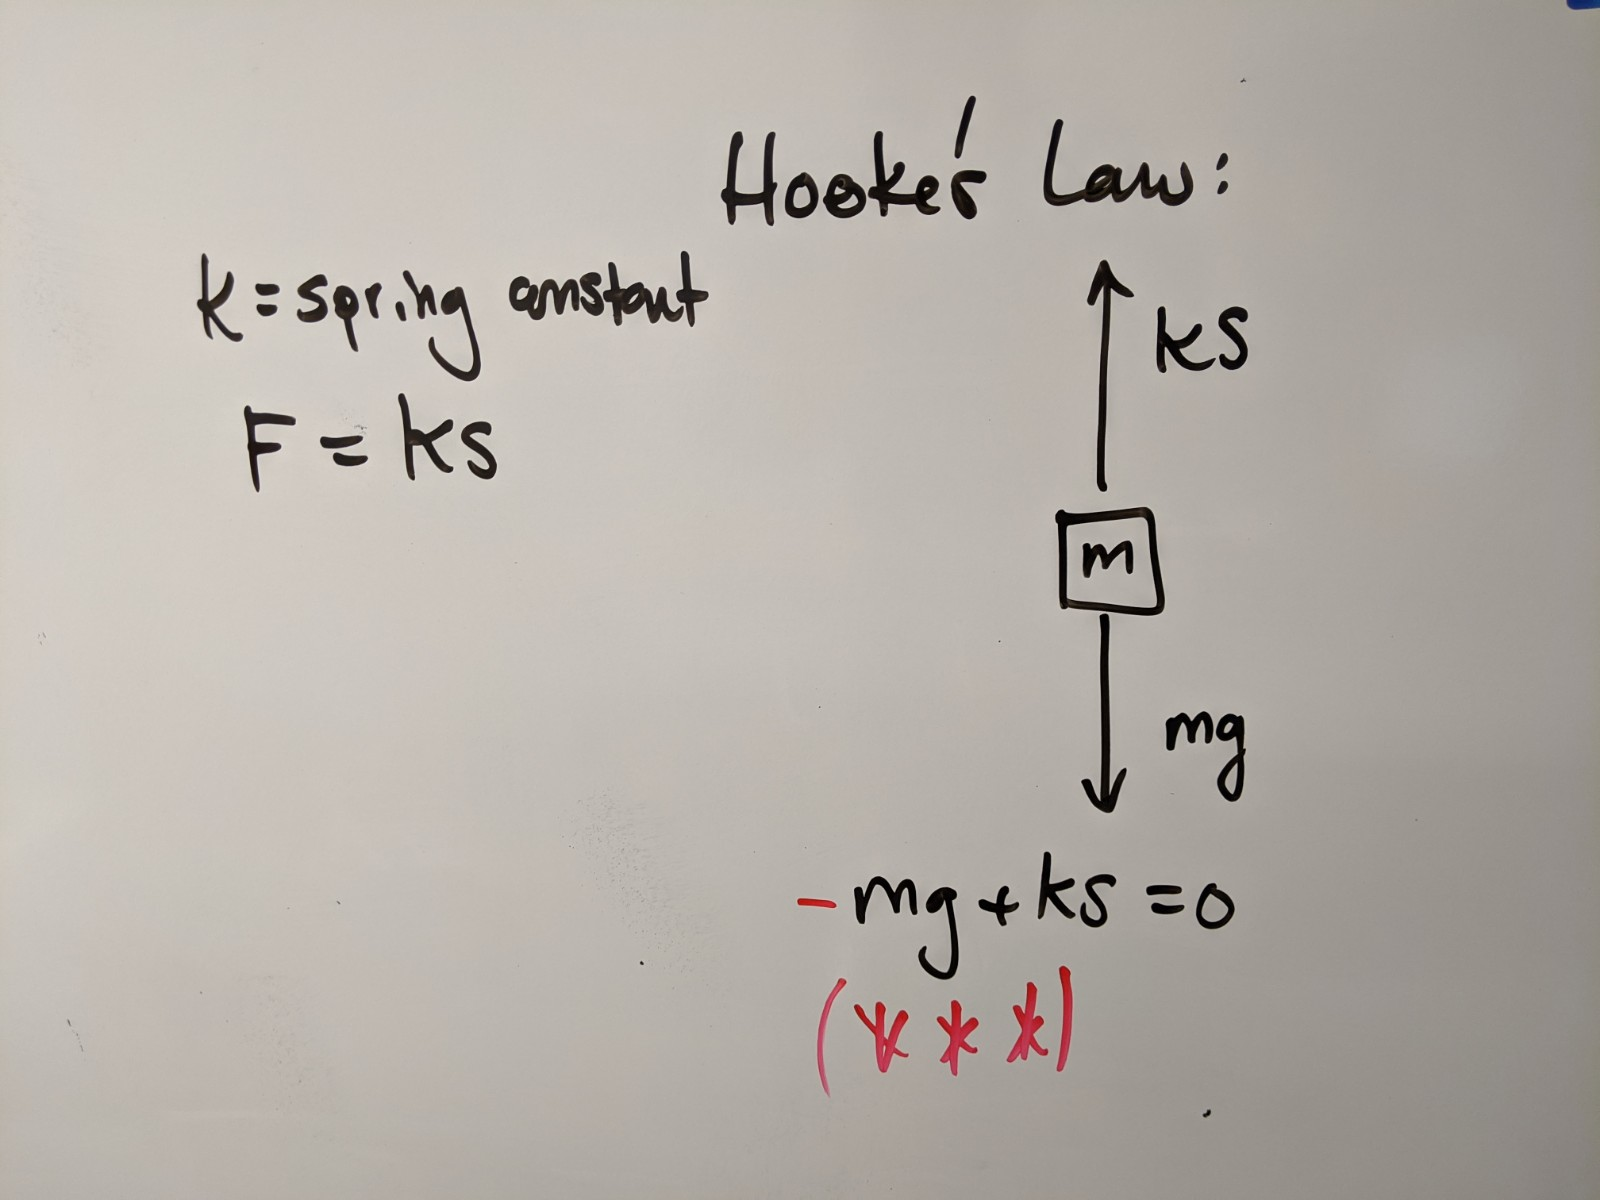
\includegraphics[width=\linewidth]{images/hookes.jpg}
\end{image}%
\begin{image}{0}{1}{0}%
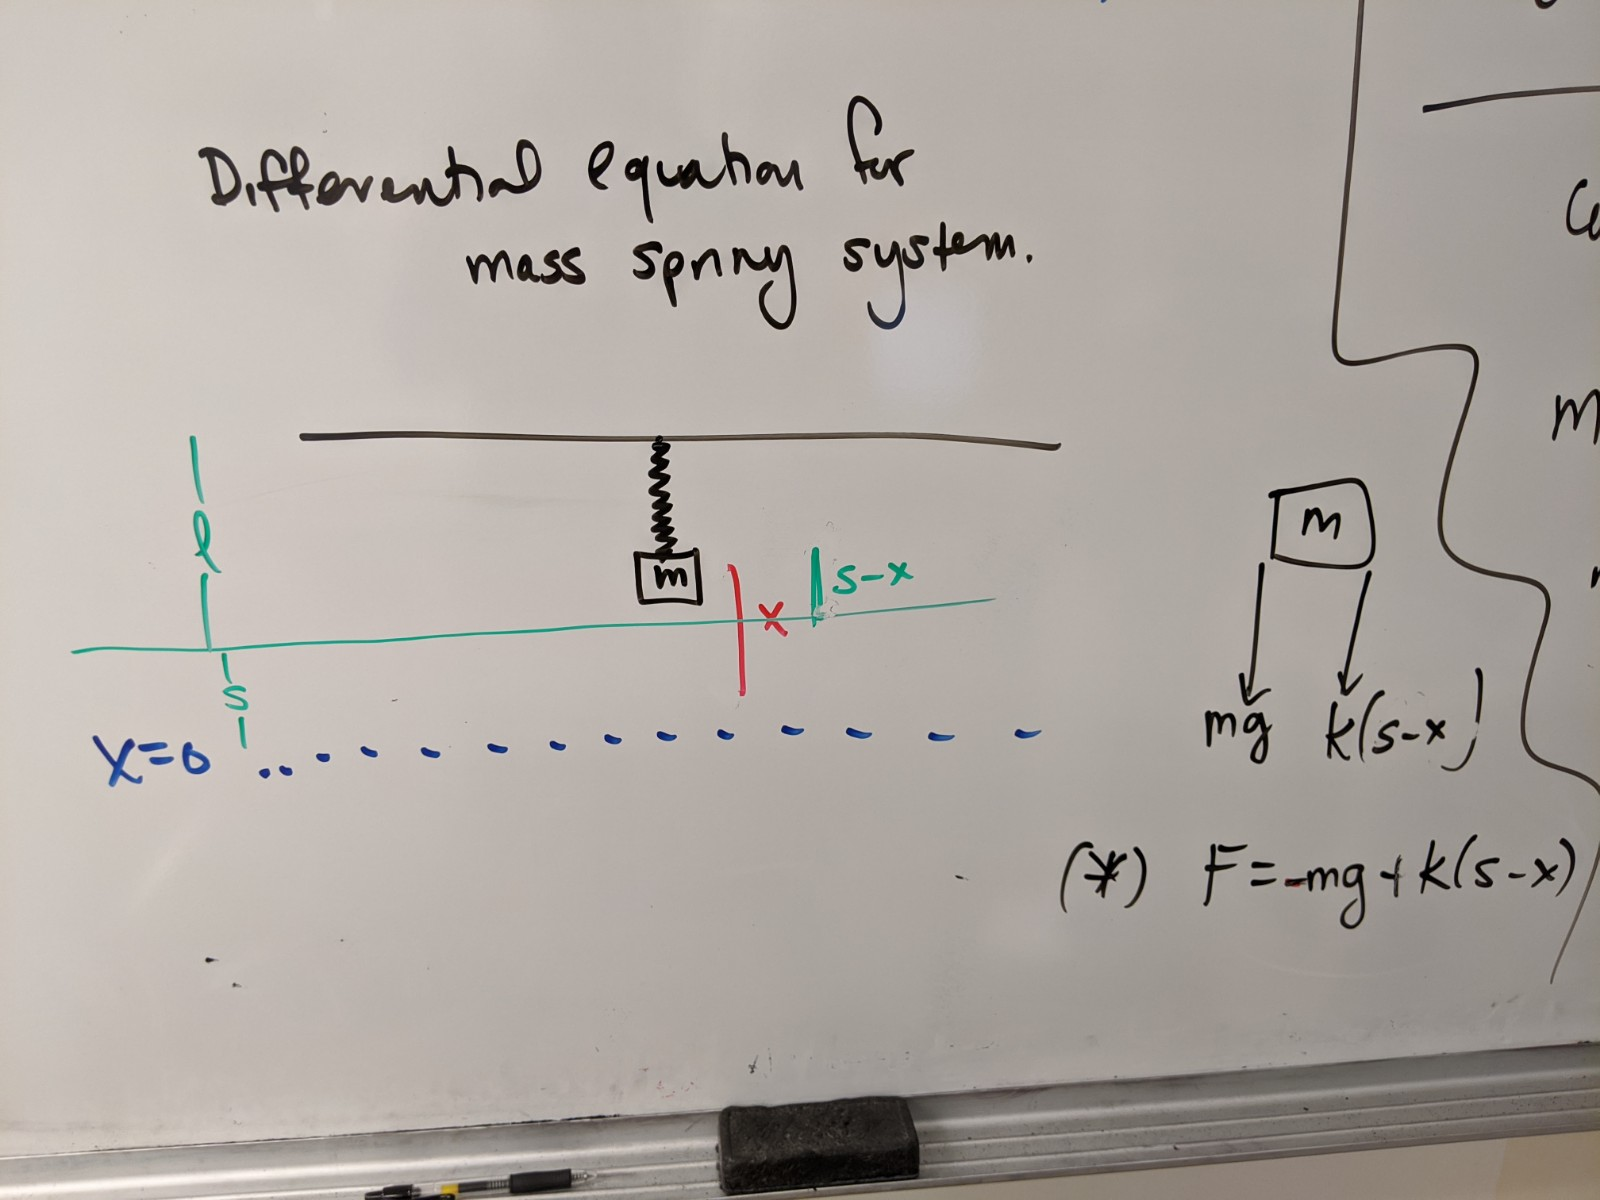
\includegraphics[width=\linewidth]{images/spring_diff_1.jpg}
\end{image}%
\begin{image}{0}{1}{0}%
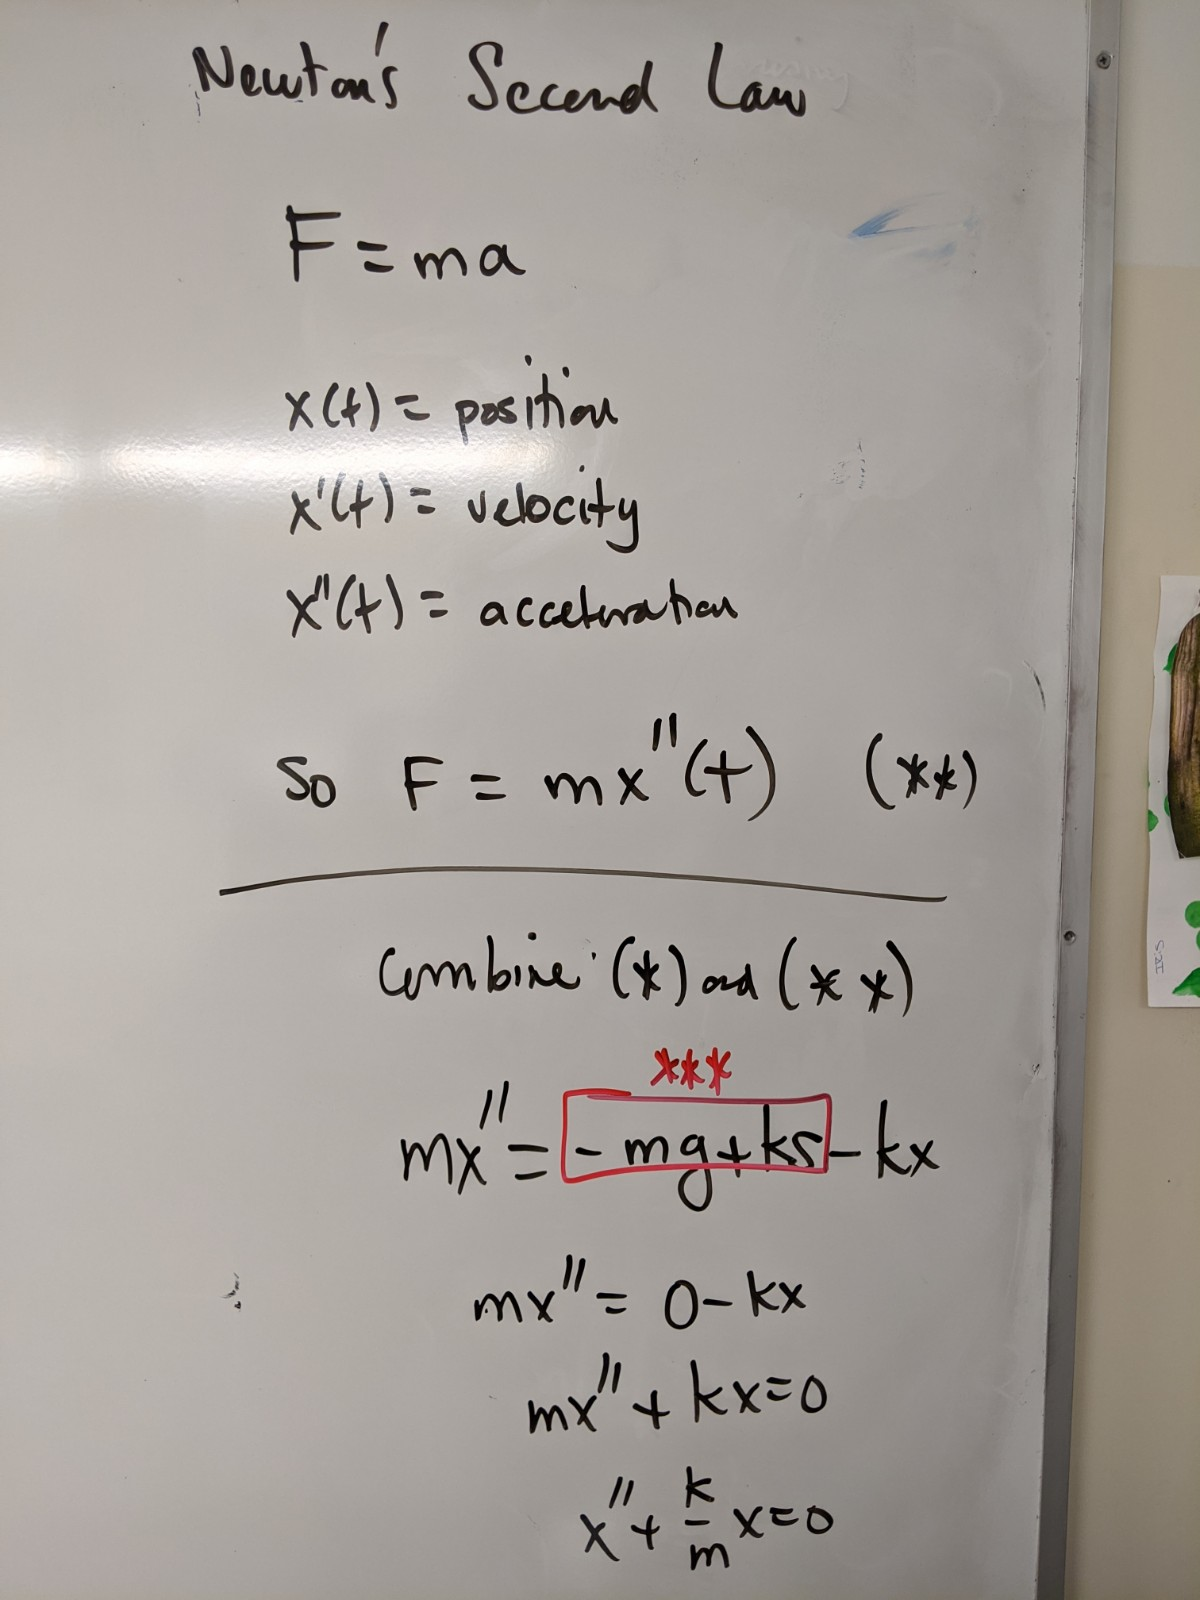
\includegraphics[width=\linewidth]{images/spring_diff_2.jpg}
\end{image}%
The pictures above are a derivation of the differential equation for a simple \terminology{mass-spring system}. Notice that the resulting equation has a second derivative \(x''\) in it - thus, this is a second order equation where the position of the mass \(x(t)\) relative to the equilibrium position is a function of time \(t\):%
\begin{equation*}
x'' + \frac{k}{m} x = 0.
\end{equation*}
Also, note the important fact that the equation is linear and has constant coefficients. If we want to describe how the solutions to this equation behave, we should study second order equations with constant coefficients.%
\end{subsectionptx}
%
%
\typeout{************************************************}
\typeout{Subsection 3.1.2 Damped mass-spring systems}
\typeout{************************************************}
%
\begin{subsectionptx}{Damped mass-spring systems}{}{Damped mass-spring systems}{}{}{g:subsection:id332532}
One way to model more complicated situations with a mass-spring system is to include a \terminology{damper} that applies force against the direction of motion. The spring\slash{}shock absorber system in a car wheel is an example of a \terminology{damped mass-spring system}. The pictures below derive the equation for this in the case that we assume that the damper exerts a force proportional to and in the opposite direction from the velocity of the mass.%
\begin{image}{0}{1}{0}%
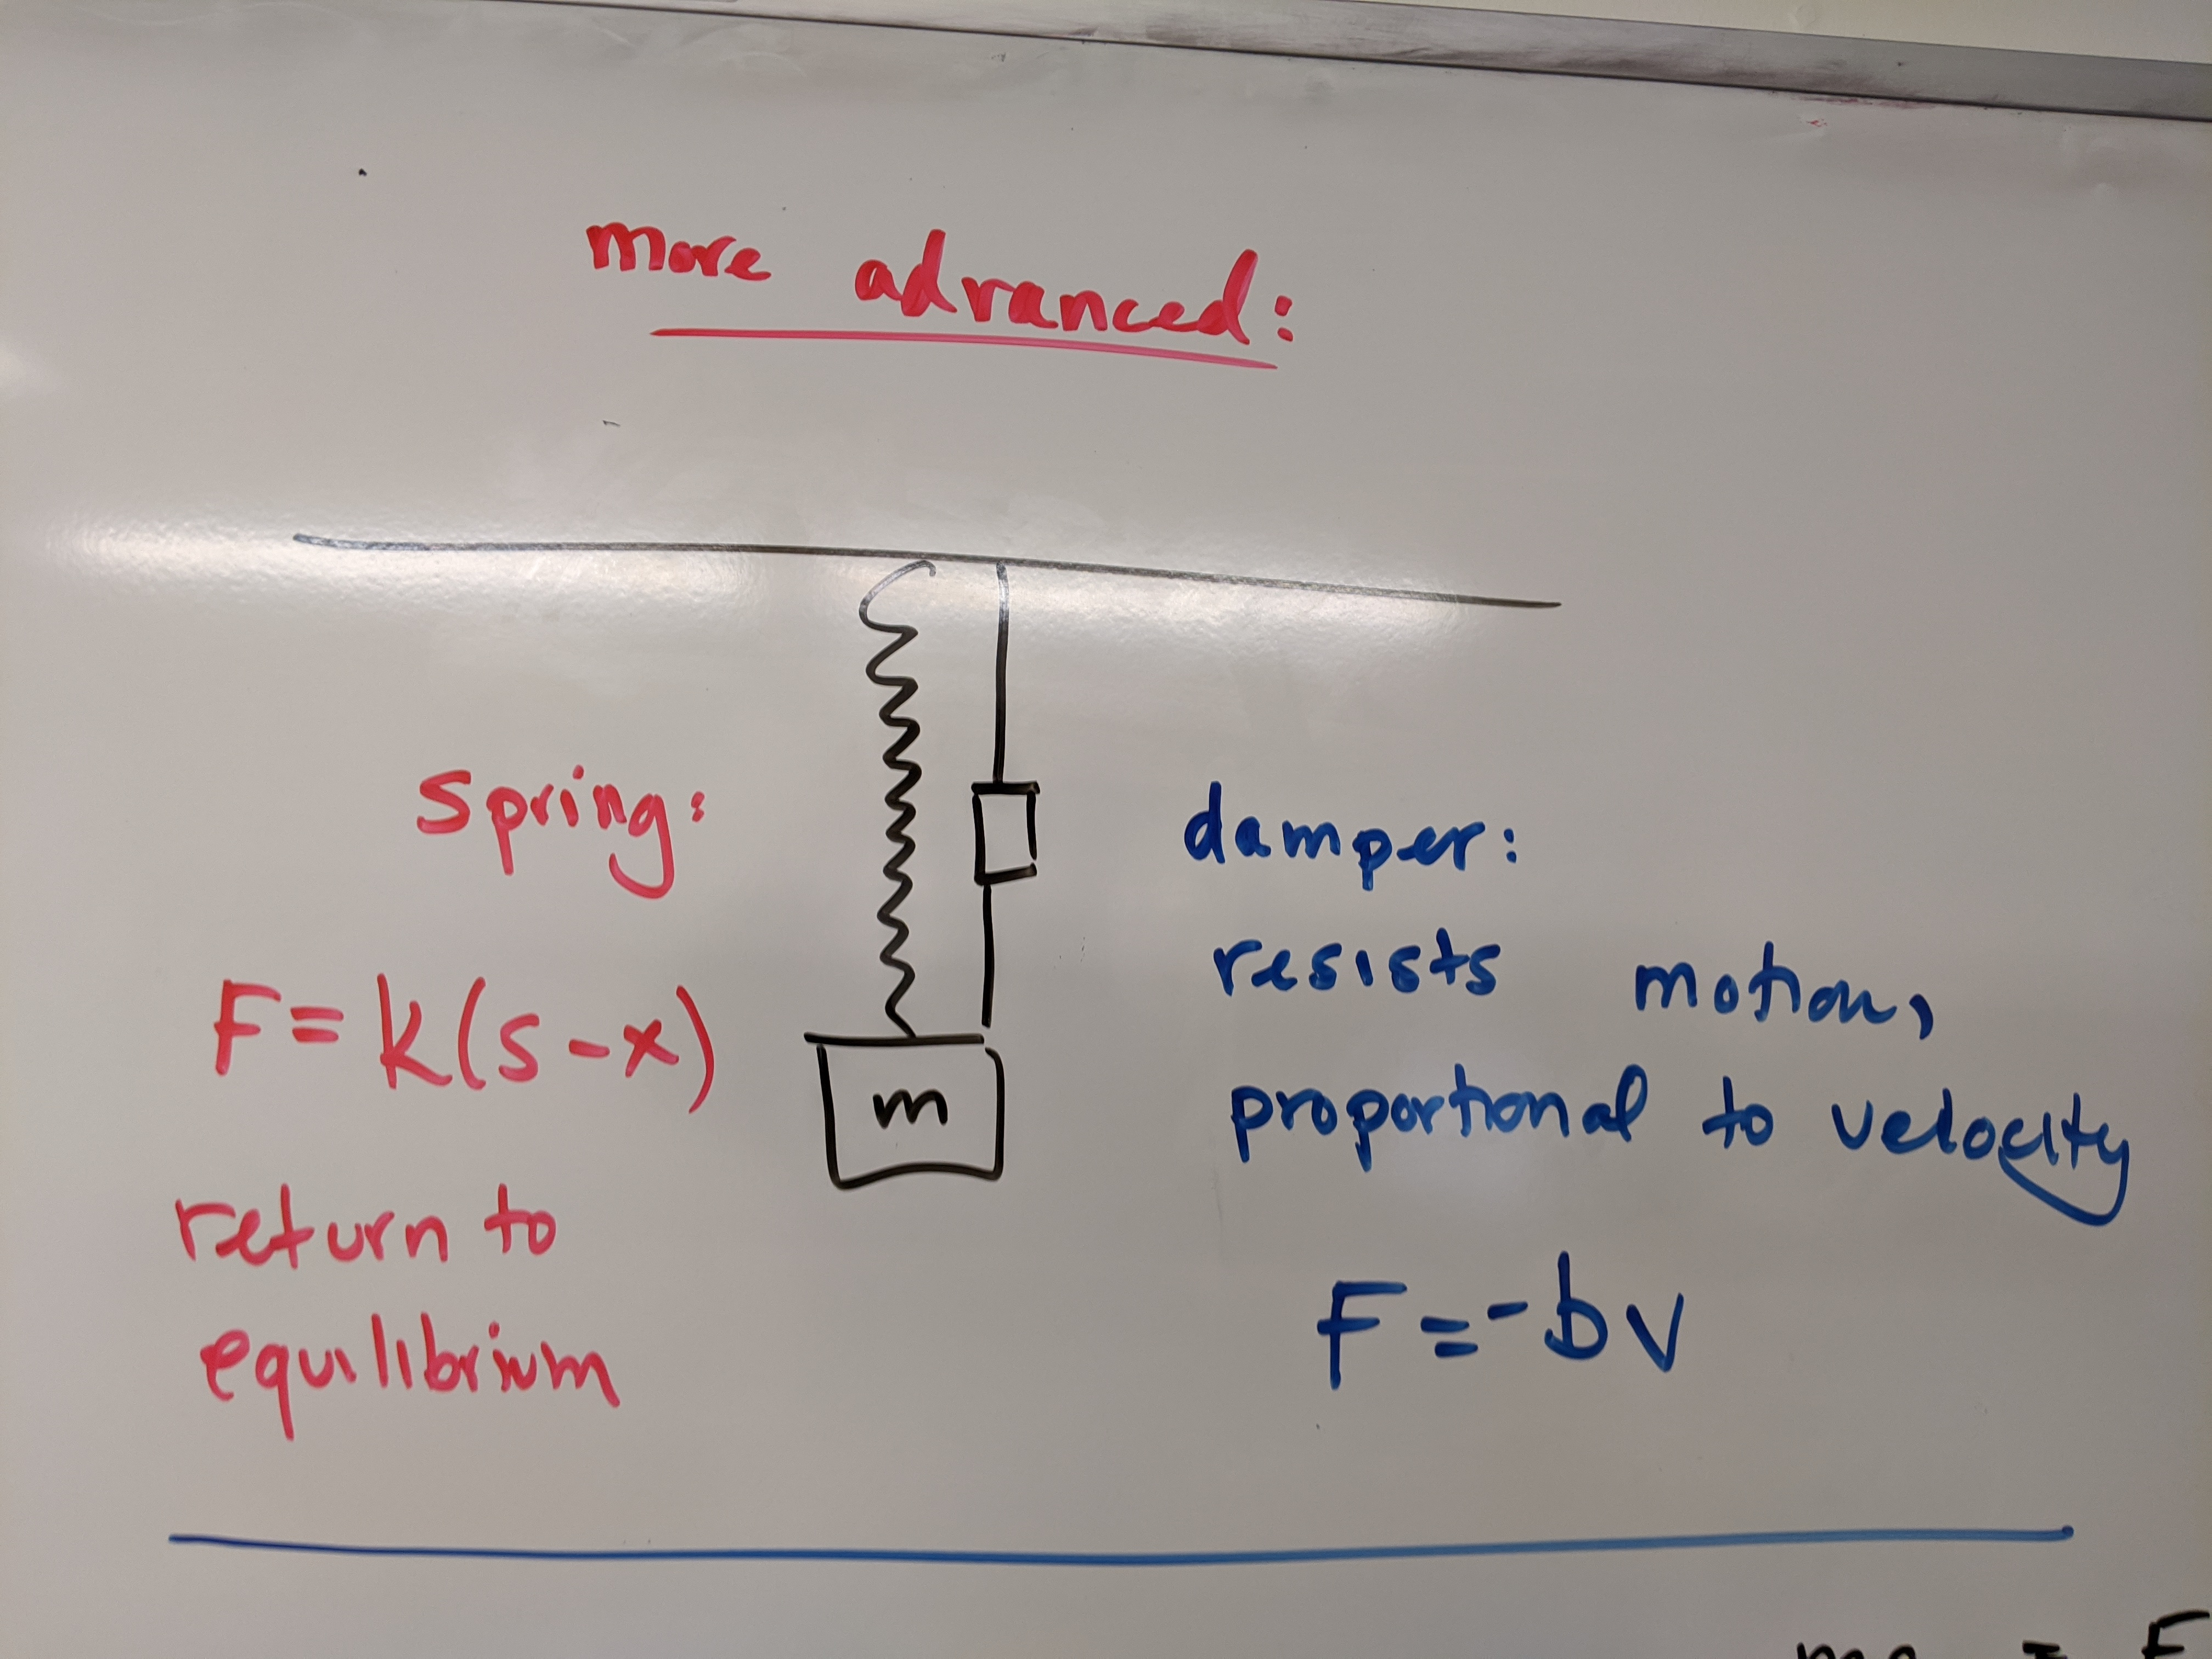
\includegraphics[width=\linewidth]{images/damped1.jpg}
\end{image}%
\begin{image}{0}{1}{0}%
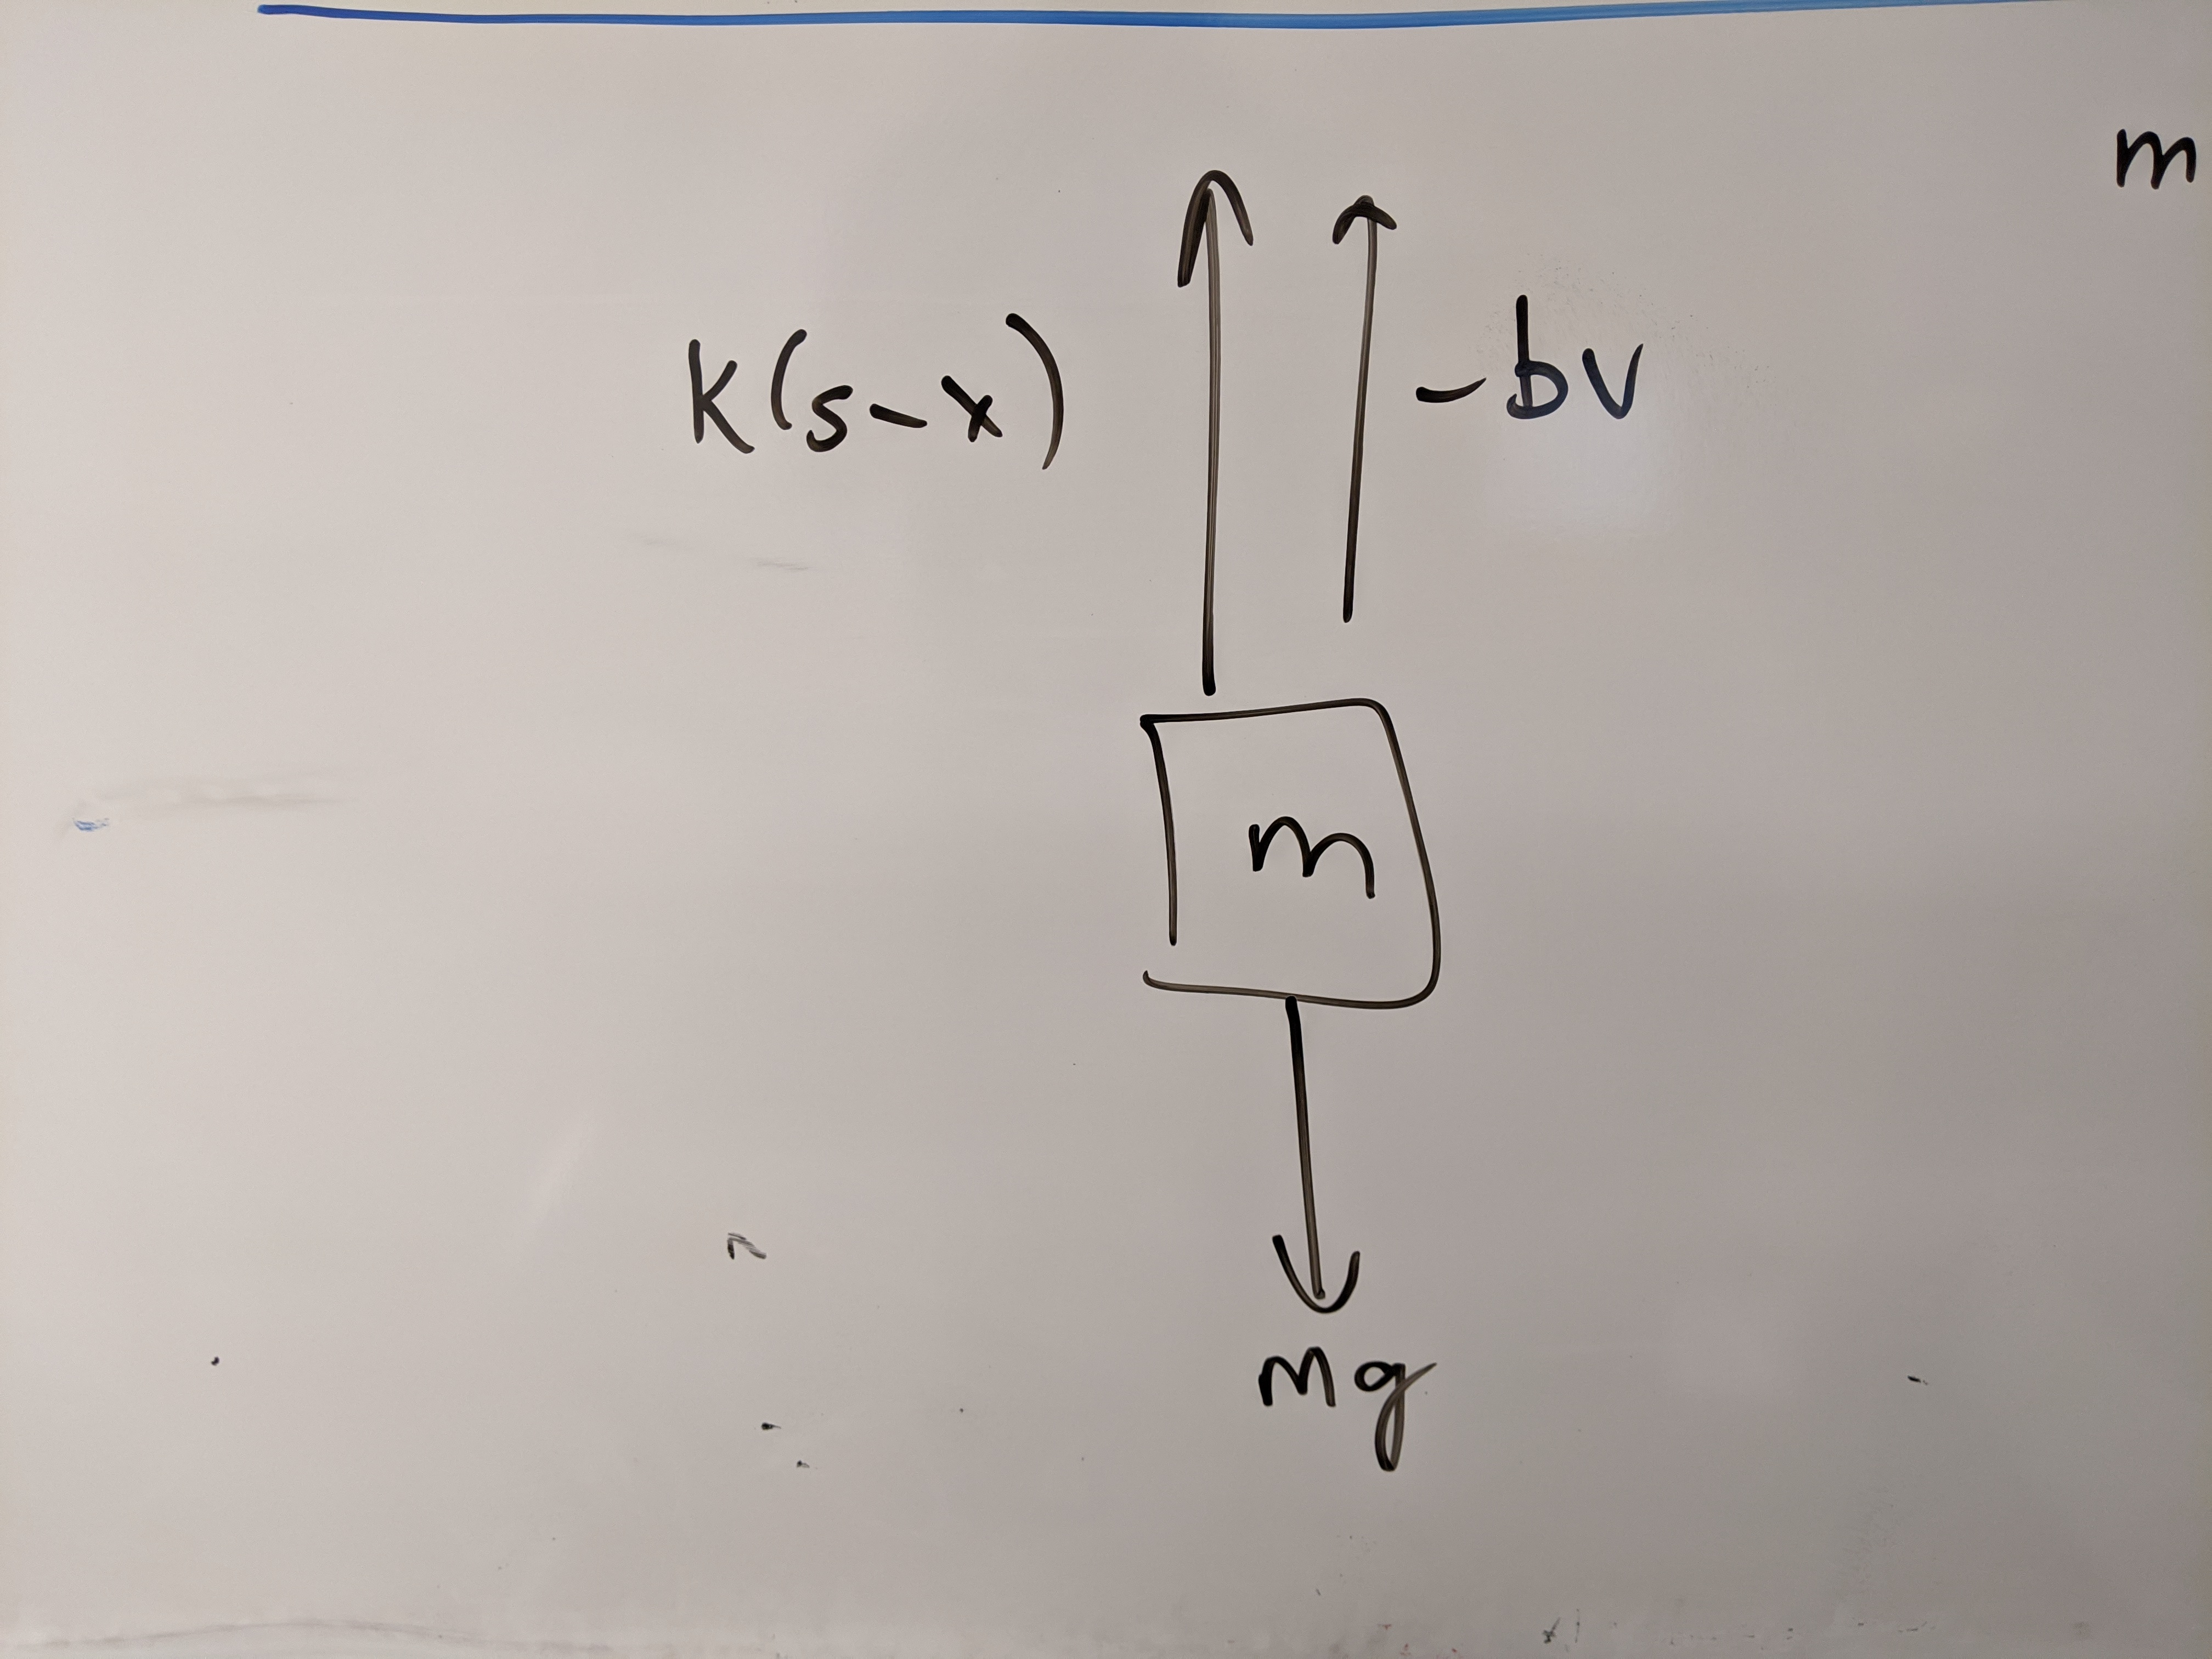
\includegraphics[width=\linewidth]{images/damped2.jpg}
\end{image}%
\begin{image}{0}{1}{0}%
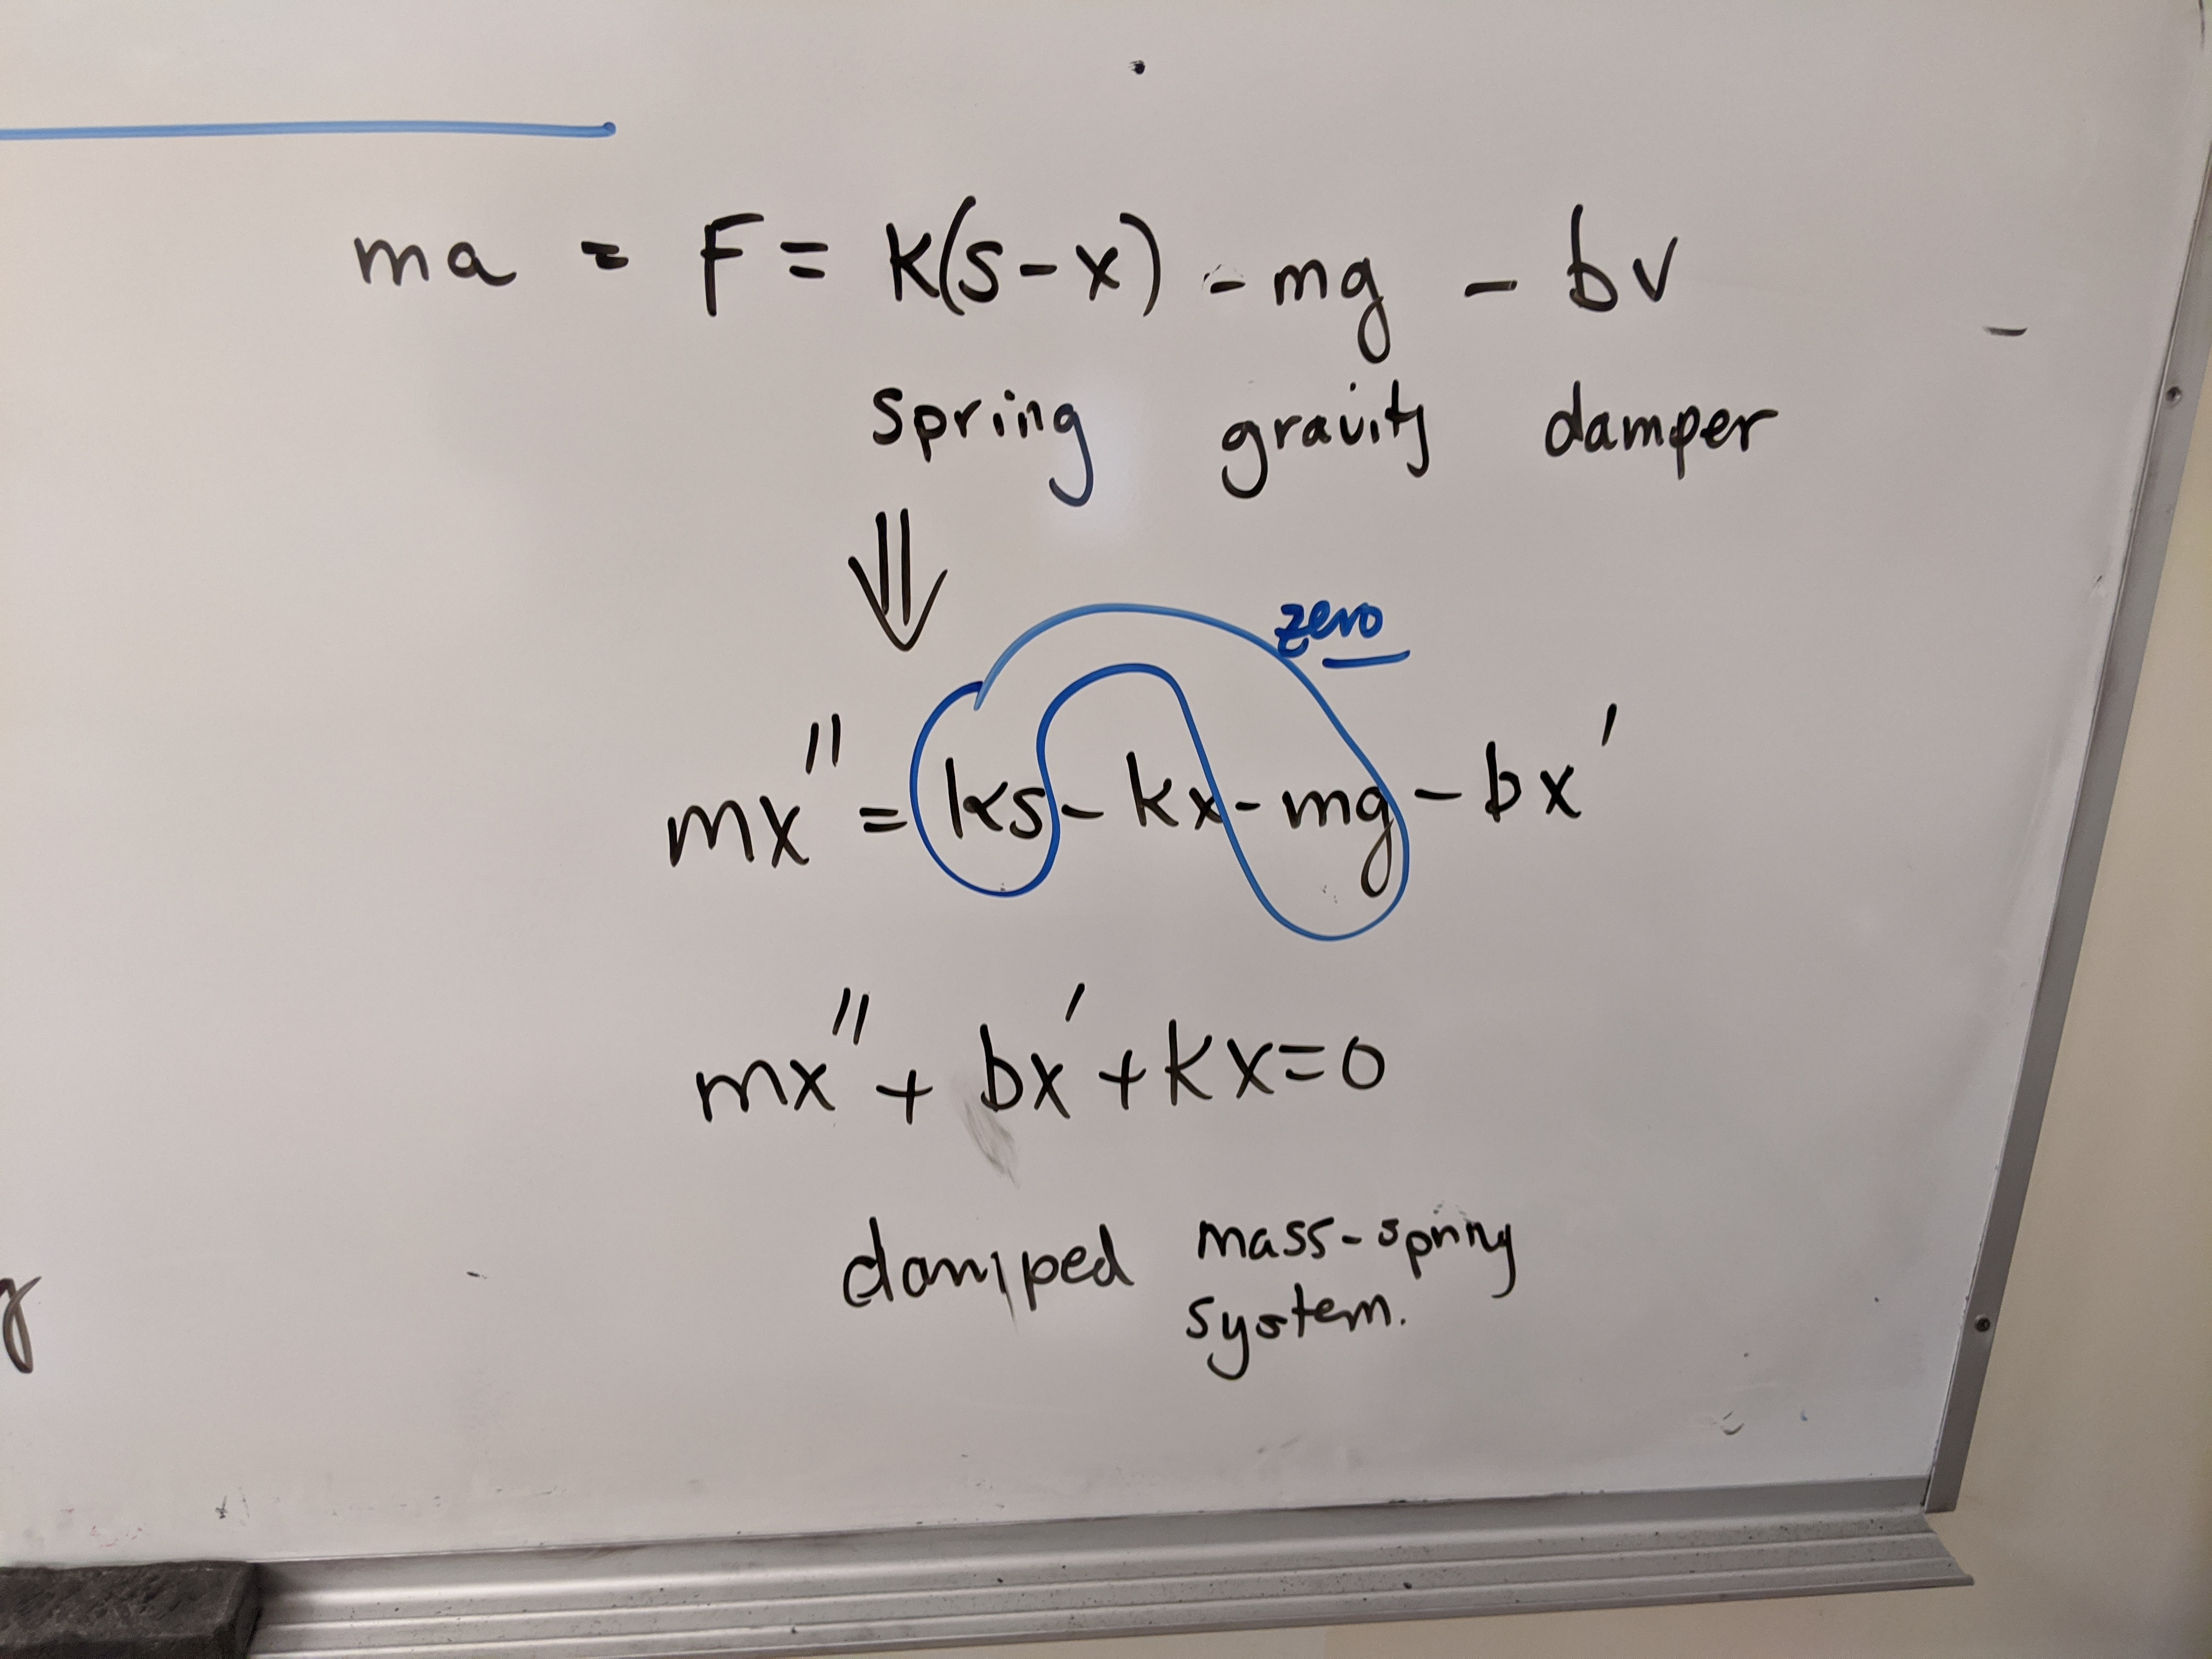
\includegraphics[width=\linewidth]{images/damped3.jpg}
\end{image}%
Thus, the equation for a damped mass-spring system is%
\begin{equation*}
x'' + \frac{b}{m} x' + \frac{k}{m} x = 0
\end{equation*}
which is also a second order linear equation with constant coefficients.%
\par
The mass-spring system is one of the most useful models in all of science. For example, RLC circuits (resistor\slash{}inductor\slash{}capacitor) are typically modeled as mass-spring systems.%
\par
This motivates the study of second order linear differential equations with constant coefficients, even though that might seem like an extremely restricted family of problems to think about. In later sections, we will extend our ideas to consider what happens if an external \emph{driving} or \emph{forcing function} is applied to the system.%
\par
We should already have an idea about the sorts of functions that solve these systems.%
\begin{enumerate}
\item{}Physical intuition tells us that when we release a mass attached to a spring from a non-equilibrium starting position, the mass oscillates up and down around the equilibrium position. This suggests that sine or cosine waves might be involved in the solution.%
\item{}Mathematical intuition tells us that functions that are related to their second derivatives by constant factors are also sines and cosines. That is, \((\sin x)'' = - \sin x\).%
\end{enumerate}
We will see that, indeed, this intuition is correct for undamped systems with no external forces.%
\end{subsectionptx}
\end{sectionptx}
%
%
\typeout{************************************************}
\typeout{Section 3.2 Second order linear equations}
\typeout{************************************************}
%
\begin{sectionptx}{Second order linear equations}{}{Second order linear equations}{}{}{x:section:ch3-2}
\begin{introduction}{}%
A \terminology{general second order ODE} is of the form%
\begin{equation*}
\frac{d^{2}y}{dt^{2}}=f\left(t,y,\frac{dy}{dt}\right).
\end{equation*}
As is the case with first order equations, we can describe a more structured family of equations. A \terminology{\(2^{nd}\) order linear ODE} is of the form%
\begin{equation*}
a(t)y^{\prime\prime}+b(t)y^{\prime}+c(t)y=d(t)
\end{equation*}
which can be rewritten as%
\begin{equation*}
y^{\prime\prime}+p(t)y^{\prime}+q(t)y=g(t).
\end{equation*}
A 2nd order ODE is called \terminology{homogeneous} if%
\begin{equation*}
a(t)y^{\prime\prime}+b(t)y^{\prime}+c(t)y=0
\end{equation*}
and \terminology{nonhomogeneous} if%
\begin{equation*}
a(t)y^{\prime\prime}+b(t)y^{\prime}+c(t)y=d(t)
\end{equation*}
for some \(d(t)\) that is NOT identically zero.%
\par
An intial value problem for a second order ODE needs to have \alert{two} initial conditions:%
\begin{align*}
y(t_{0}) \amp =y_{0},\\
y^{\prime}(t_{0}) \amp =y_{0}^{\prime}.
\end{align*}
%
\end{introduction}%
%
%
\typeout{************************************************}
\typeout{Subsection 3.2.1 Second order linear homogeneous ODEs with constant coefficients (characteristic equation)}
\typeout{************************************************}
%
\begin{subsectionptx}{Second order linear homogeneous ODEs with constant coefficients (characteristic equation)}{}{Second order linear homogeneous ODEs with constant coefficients (characteristic equation)}{}{}{g:subsection:id332834}
We will begin with the \terminology{2nd order linear homogeneous ODEs with constant coefficients} that we introduced and motivated in the previous section:%
\begin{equation*}
ay''+by^{\prime}+cy=0
\end{equation*}
where \(a,b,c\) are real constants.%
\par
Consider \(y^{\prime\prime}-y=0\) or%
\begin{equation*}
y^{\prime\prime}=y.
\end{equation*}
Can we think of a solution to this ODE from Calculus 1? A function where its second derivative is equal to itself?%
\par
A moment of thought should lead us to conclude that there are two obvious solutions: \(y_{1}(t)=e^{t}\) and \(y_{2}(t)=e^{-t}\). But it not hard to check that the larger family of functions \(y = c_{1}e^{t}\) and \(y = c_{2}e^{-t}\) are also solutions for any constants \(c_1, c_2\).%
\par
Now consider the general ODE%
\begin{equation*}
ay^{\prime\prime}+by^{\prime}+cy=0.
\end{equation*}
%
\par
Guided by our observation about the solutions to the previous equation, let us assume solutions are of the form \(y(t)=e^{rt}\). (If this is an unsatisfying assumption, another appoach will be explained shortly).  Then%
\begin{align*}
y(t) \amp =e^{rt}\\
y^{\prime}(t) \amp =re^{rt}\\
y^{\prime\prime}(t) \amp =r^{2}e^{rt},
\end{align*}
and plugging this into the ODE we have%
\begin{align*}
LHS=ar^{2}e^{rt}+bre^{rt}+ce^{rt} \amp \overset{?}{=}0\\
e^{rt}\left(ar^{2}+br+c\right) \amp \overset{?}{=}0.
\end{align*}
and since \(e^{rt}\neq0\) then%
\begin{equation*}
ar^{2}+br+c=0.
\end{equation*}
Using standard methods for quadratic equations, we can solve for the roots \(r=r_{1},r_{2}\).%
\par
This is called the \terminology{characteristic equation} of this ODE. If the roots \(r_1, r_2\) are \emph{real and distinct}, then the \terminology{general solution to the homogeneous equation} is of the form%
\begin{equation*}
y(t)=c_{1}e^{r_{1}t}+c_{2}e^{r_{2}t}.
\end{equation*}
%
\par
The justification for gluing together the solutions will be presented in the next section as the ``principle of superposition''.%
\begin{example}{}{g:example:id333122}%
Let's find the general solution of%
\begin{equation*}
y^{\prime\prime}+5y^{\prime}+6y=0.
\end{equation*}
%
%
\begin{enumerate}
\item{}We'll guess that the solution to a solution is \(y(t)=e^{rt}\) for some \(r\). Then get%
\begin{equation*}
\left(r^{2}+5r+6\right)e^{rt}=0
\end{equation*}
so that we must have \(r^{2}+5r+6=\left(r+2\right)\left(r+3\right)=0\) so that \(r=-2,-3\).%
\item{}So \(y_{1}(t)=e^{-2t}\) and \(y_{2}(t)=e^{-3t}\) are solutions and%
\begin{equation*}
y(t)=c_{1}e^{-2t}+c_{2}e^{-3t}
\end{equation*}
is the general solution.%
\end{enumerate}
\end{example}
\begin{example}{}{g:example:id333186}%
Let's find the solution to the following IVP%
\begin{equation*}
y^{\prime\prime}+5y^{\prime}+6y=0\,\,\,\,y(0)=2,y^{\prime}(0)=-1.
\end{equation*}
%
\par
Solving for the particular solution. We have \(y(0)=2\) and \(y^{\prime}(0)=-1\). Differentiating \(y(t)=c_{1}e^{-2t}+c_{2}e^{-3t}\) we get \(y^{\prime}(t)=-2c_{1}e^{-2t}-3c_{2}e^{-3t}\) and set up the following system:%
\begin{align*}
c_{1}+c_{2} \amp = \amp 2\\
-2c_{1}-3c_{2} \amp = \amp -1
\end{align*}
and get \(c_{1}=5,c_{2}=-3\). So the particular solution is%
\begin{equation*}
y(t)=5e^{-2t}-3e^{-3t}.
\end{equation*}
%
\end{example}
\begin{example}{}{g:example:id333277}%
Let's find the general solution of%
\begin{equation*}
2\frac{d^{2}y}{dt^{2}}+7\frac{dy}{dt}-4y=0.
\end{equation*}
%
%
\begin{enumerate}
\item{}We'll guess that the solution to a solution is \(y(t)=e^{rt}\) for some \(r\). Then get%
\begin{equation*}
\left(2r^{2}+7r-4\right)e^{rt}=0
\end{equation*}
so that we must have \(2r^{2}+7r-4=\left(2r-1\right)\left(r+4\right)=0\) so that \(r=\frac{1}{2},-4\).%
\item{}So \(y_{1}(t)=e^{t/2}\) and \(y_{2}(t)=e^{-4t}\) are solutions and%
\begin{equation*}
y(t)=c_{1}e^{t/2}+c_{2}e^{-4t}
\end{equation*}
is the general solution.%
\end{enumerate}
\end{example}
\end{subsectionptx}
%
%
\typeout{************************************************}
\typeout{Subsection 3.2.2 Derivatives as linear operators and the characteristic equation}
\typeout{************************************************}
%
\begin{subsectionptx}{Derivatives as linear operators and the characteristic equation}{}{Derivatives as linear operators and the characteristic equation}{}{}{g:subsection:id333415}
It might seem unsatisfying to assume the form of an answer and then show that our guess worked. Is there a mathematical justification for making this guess? The answer is yes, if we're willing to push our understanding of differentiation slightly.%
\par
Define the \terminology{differential operator} \(D\) to be the operation of applying \(\frac{d}{dx}\) to a function \(y(x)\). The operator \(D\) can be thought of as a function on functions:%
\begin{equation*}
D(\text{function}) = \text{ derivative}.
\end{equation*}
Any order of derivative can be thought of this way. For example,%
\begin{equation*}
y''' = \frac{d^3 y}{dx^3} = \frac{d^3}{dx^3} y = D^3 y.
\end{equation*}
We need a notion of \(D^0\) - what should that mean? It makes sense to set \(D^0(y) = y\) - that is, take no derivatives of \(y\). We will use the symbol \(1\) to represent this function, the \terminology{identity function} that leaves \(y\) unchanged.%
\par
In Calculus, we learn that derivatives follow certain rules. Two of the most important are%
\begin{equation*}
D(f + g) = Df + Dg
\end{equation*}
and%
\begin{equation*}
D(cf) = cD(f).
\end{equation*}
These two properties together show that \(D\) is a \terminology{linear function}.%
\par
Using differential operator notation allows us to transform an ODE and use algebraic techniques to solve it using first order methods. Consider the equation%
\begin{equation*}
y'' + 3 y ' + 2 y = 0.
\end{equation*}
This can be written%
\begin{equation*}
D^2 y + 3 D y + 2 y = 0
\end{equation*}
using operator notation. But since each operator is applied to the same input, \(y\), we can use function notation to write%
\begin{equation*}
(D^2 + 3D + 2)(y) = 0.
\end{equation*}
%
\par
The operator expression \(D^2 + 3D + 2\) can be factored as symbols into \((D + 2)(D + 1)\) (that this is equal to the original equation applied to \(y\) is a consequence of linearity). Now, using the fact that the derivative of 0 is 0, we assert that the solutions to the equation%
\begin{equation*}
(D + 1)(D + 2)y = (D + 2)(D+1)y = 0
\end{equation*}
are the solutions to \((D + 1)(y) = 0\) and \((D + 2)y = 0\), which are just the first order equations%
\begin{gather*}
y' + y = 0\\
y' + 2y = 0
\end{gather*}
These are separable, with solutions \(y_1 = c_1 e^{-x}\) and \(y_2 = c_2 e^{-2x}\). So the general solution (justified by the principle of superposition, covered in the next section) to the ODE is%
\begin{equation*}
y = c_1 e^{-x} + c_2 e^{-2x}.
\end{equation*}
%
\par
Note that the operator polynomial \(D^2 + 3D + 2\) is precisely equivalent to the characteristic polynomial \(r^2 + 3r + 2\).%
\end{subsectionptx}
\end{sectionptx}
%
%
\typeout{************************************************}
\typeout{Section 3.3 Solutions to Linear Equations; the Wronskian}
\typeout{************************************************}
%
\begin{sectionptx}{Solutions to Linear Equations; the Wronskian}{}{Solutions to Linear Equations; the Wronskian}{}{}{x:section:ch3-3}
\begin{introduction}{}%
In this section, we will consider equations of the form%
\begin{equation*}
y^{\prime\prime}+p(t)y^{\prime}+q(t)y=0,\,\,\,\,\,y(t_{0})=y_{0},\,\,\,\,y^{\prime}(t_{0})=y_{0}^{\prime}.
\end{equation*}
where \(a,b,c\) are constants. This is a second order, linear, homogeneous equation. Our goal is to find the general solution of these equations.%
\begin{theorem}{(Existence and Uniqueness for \(2\)nd order linear ODES).}{}{x:theorem:thm2ndexist}%
Consider the IVP%
\begin{equation*}
y^{\prime\prime}+p(t)y^{\prime}+q(t)y=g(t),\,\,\,\,\,y(t_{0})=y_{0},\,\,\,\,y^{\prime}(t_{0})=y_{0}^{\prime}
\end{equation*}
where \(p,q,g\) are continuous on an open interval \(I\) that contains \(t_{0}\). Then there exists a unique solution \(y=\phi(t)\), and the solution exists throughout all of \(I\).%
\end{theorem}
Recall that this theorem implies that a solution to this IVP%
\begin{enumerate}
\item{}exists,%
\item{}is unique%
\item{}and the solution \(\phi\) is defined throughout all of \(I\).%
\end{enumerate}
In fact it says more, namely that \(\phi\) is at least twice differentiable on \(I\).%
\begin{example}{}{g:example:id498118}%
Find the longest interval in which the solution to the IVP is certain to exist by \hyperref[x:theorem:thm2ndexist]{Theorem~{\xreffont\ref{x:theorem:thm2ndexist}}}:%
\begin{equation*}
\left(t^{4}-4t^{2}\right)y^{\prime\prime}+\cos ty^{\prime}-e^{t}y=0,\,\,\,\,\,\,y(1)=2,\,\,\,y^{\prime}(1)=1.
\end{equation*}
%
\par
\alert{Solution:} Rewrite the equation as%
\begin{equation*}
y^{\prime\prime}+\frac{\cos t}{t^{2}\left(t^{2}-4\right)}y^{\prime}-\frac{e^{t}}{t^{2}\left(t^{2}-4\right)}y=0.
\end{equation*}
so that \(p(t)=\frac{\cos t}{t^{2}\left(t^{2}-4\right)}\) and \(q(t)=-\frac{e^{t}}{t^{2}\left(t^{2}-4\right)}\) which are both continuous on \(\left(-\infty,-2\right)\cup\left(-2,0\right)\cup\left(0,2\right)\cup\left(2,\infty\right)\). Since \(t_{0}=1\in\left(0,2\right)\) then \(I=\left(0,2\right)\) is the longest interval where \(p(t)\) and \(q(t)\) are both continuous that contains \(t_{0}\).%
\end{example}
\end{introduction}%
%
%
\typeout{************************************************}
\typeout{Subsection 3.3.1 Principle of Superposition}
\typeout{************************************************}
%
\begin{subsectionptx}{Principle of Superposition}{}{Principle of Superposition}{}{}{g:subsection:id498330}
We now give a name to idea that linear combinations of solutions to a linear homogeneous differential equation remain solutions. (Again, the underlying principle is the linearity of the differential operator.)%
\begin{theorem}{Superposition of solutions to linear homogeneous ODE.}{}{g:theorem:id498338}%
If \(y_{1}\) and \(y_{2}\) are two solutions to an ODE%
\begin{equation*}
y^{\prime\prime}+p(t)y^{\prime}+q(t)y=0,
\end{equation*}
then the linear combination \(y(t)=c_{1}y_{1}(t)+c_{2}y_{2}(t)\) is also a solution for any values \(c_{1},c_{2}\).%
\end{theorem}
\alert{Warning:} The principle of superposition holds only if the equation is \emph{linear} and \emph{homogeneous}.%
\begin{example}{}{g:example:id498628}%
Suppose \(y_{1}(t)=e^{-t}\) and \(y_{2}(t)=e^{t}\) are two solutions to \(y^{\prime\prime}-y=0\). Since this is a linear homogeneous ODE then the principle of superposition says that the function%
\begin{equation*}
y(t)=2e^{-t}+3e^{t}
\end{equation*}
is also a solution.%
\end{example}
\begin{example}{}{g:example:id498732}%
It is not hard to check that \(y_{1}(t)=1\) and \(y_{2}(t)=t^{\frac{1}{2}}\) are solutions to%
\begin{equation*}
yy^{\prime\prime}+\left(y^{\prime}\right)^{2}=0,\,\,\,t>0.
\end{equation*}
%
\par
Part (a): Show \(y(t)=1+2t^{\frac{1}{2}}\) is not a solution to this ODE:%
\par
Solution: First compute%
\begin{align*}
y(t) \amp =1+2t^{\frac{1}{2}}\\
y^{\prime}(t) \amp =t^{-\frac{1}{2}}\\
y^{\prime\prime}(t) \amp =-\frac{1}{2}t^{-\frac{3}{2}}
\end{align*}
To show this simply check if the LHS equal to \(0\):%
\begin{align*}
LHS \amp =yy^{\prime\prime}+\left(y^{\prime}\right)^{2}=\left(1+2t^{\frac{1}{2}}\right)\left(-\frac{1}{2t^{3/2}}\right)+\left(\frac{1}{t^{\frac{1}{2}}}\right)^{2}\\
\amp =-\frac{1}{2t^{3/2}}-\frac{1}{t}+\frac{1}{t}=-\frac{1}{2t^{3/2}}\neq0,
\end{align*}
%
\par
Part (b): Why does this not contradict the Principle of Superposition?%
\par
Solution: To apply the principle, the equation needs to be linear. The term \(\left(y^{\prime}\right)^{2}\) in the ODE makes this nonlinear, hence we can't even use the principle in the first place.%
\end{example}
\end{subsectionptx}
%
%
\typeout{************************************************}
\typeout{Subsection 3.3.2 Fundamental sets of solutions}
\typeout{************************************************}
%
\begin{subsectionptx}{Fundamental sets of solutions}{}{Fundamental sets of solutions}{}{}{g:subsection:id499031}
Suppose that \(y_{1}(t)\) and \(y_{2}(t)\) are two solutions to a second order linear homogeneous equation. When do we know that%
\begin{equation*}
y(t)=c_{1}y_{1}(t)+c_{2}y_{2}(t)
\end{equation*}
is the \terminology{general solution} to the ODE? That is, when do we know that we can obtain \emph{every single solution} to an IVP? To answer that we need to define some machinery.%
\begin{definition}{}{g:definition:id499150}%
The determinant of a matrix \(\left(\begin{array}{cc}
a \amp b\\
c \amp d
\end{array}\right)\) is%
\begin{equation*}
\left|\begin{array}{cc}
a \amp b\\
c \amp d
\end{array}\right|=ad-bc.
\end{equation*}
\end{definition}
\begin{definition}{}{g:definition:id499143}%
The \terminology{Wronskian} of the solutions \(y_{1}(t)\) and \(y_{2}(t)\) to a second order linear homogeneous ODE is the function%
\begin{equation*}
W=W(y_{1},y_{2})(t)=\left|\begin{array}{cc}
y_{1}(t) \amp y_{2}(t)\\
y_{1}^{\prime}(t) \amp y_{2}^{\prime}(t)
\end{array}\right|.
\end{equation*}
\end{definition}
The Wronskian computes a function that can be used to check of a solution set is sufficient to construct every possible solution.%
\begin{theorem}{General solution theorem.}{}{x:theorem:thmgensol}%
Suppose \(y_{1}\) and \(y_{2}\) are two solutions to the ODE%
\begin{equation*}
y^{\prime\prime}+p(t)y^{\prime}+q(t)y=0
\end{equation*}
in some interval \(I\) where \(p,q\) are continuous. Then the family of solutions%
\begin{equation*}
y(t)=c_{1}y_{1}(t)+c_{2}y_{2}(t)
\end{equation*}
for arbtitrary \(c_{1},c_{2}\) is the general solution if and only if the Wronskian \(W\left(y_{1},y_{2}\right)\) is not zero for at least one point \(t_{0}\) in \(I\).%
\end{theorem}
\begin{example}{}{g:example:id499452}%
Find the general solution to%
\begin{equation*}
y^{\prime\prime}+4y^{\prime}-5y=0.
\end{equation*}
%
\par
Solution: In the last section we showed that to find solutions to this ODE we simply need to solve the characteristic equation%
\begin{equation*}
r^{2}+4r-5=\left(r-1\right)\left(r+5\right)=0
\end{equation*}
and get \(r=1,-5\) so that%
\begin{equation*}
y(t)=c_{1}e^{t}+c_{2}e^{-5t}
\end{equation*}
gives other solutions to the ODE. To show this gives all of them, we simply need to show the Wronksian is not always zero:%
\begin{align*}
W\left(e^{t},e^{-5t}\right) \amp =\left|\begin{array}{cc}
y_{1}(t) \amp y_{2}(t)\\
y_{1}^{\prime}(t) \amp y_{2}^{\prime}(t)
\end{array}\right|=\left|\begin{array}{cc}
e^{t} \amp e^{-5t}\\
e^{t} \amp -5e^{-5t}
\end{array}\right|\\
\amp =-5e^{-4t}-e^{-4t}\\
\amp =-6e^{-4t}\\
\amp \neq0.
\end{align*}
%
\end{example}
To find the general solution of \(y^{\prime\prime}+p(t)y^{\prime}+q(t)y=g(t)\), we only need to find two (\(y_{1},y_{2}\)) solutions whose Wronskian is nonzero:%
\begin{enumerate}
\item{}First find two solutions \(y_{1},y_{2}\).%
\item{}Then check \(W(y_{1},y_{2})\neq0\) for at least one point in the interval.%
\end{enumerate}
%
\begin{definition}{}{g:definition:id499797}%
The solutions \(y_{1}\) and \(y_{2}\) are said to form a \terminology{fundamental set of solutions} to%
\begin{equation*}
y^{\prime\prime}+p(t)y^{\prime}+q(t)y=0
\end{equation*}
if \(W\left(y_{1},y_{2}\right)\neq0\).%
\end{definition}
\begin{example}{}{g:example:id499877}%
Verify that \(y_{1}(t)=t^{\frac{1}{2}}\) and \(y_{2}(t)=t^{-1}\) form a fundamental set of solutions of%
\begin{equation*}
2t^{2}y^{\prime\prime}+3ty^{\prime}-y=0,\,\,\,\,\,t>0.
\end{equation*}
%
\par
Solution:%
\par
Part (a): First we verify these are indeed solutions by plugging them into the LHS and checking that they equal zero. First computer some derivatives%
\begin{equation*}
\begin{array}{ccc}
y_{1}(t)=t^{\frac{1}{2}} \amp  \amp y_{2}(t)=t^{-1}\\
y_{2}^{\prime}(t)=\frac{1}{2}t^{-\frac{1}{2}} \amp  \amp y_{2}^{\prime}(t)=-t^{-2}\\
y_{3}^{\prime}(t)=-\frac{1}{4}t^{-\frac{3}{2}} \amp  \amp y_{2}^{\prime\prime}(t)=-t^{-2}.
\end{array}
\end{equation*}
Plugging \(y_{1}\) into LHS we get%
\begin{align*}
LHS \amp =2t^{2}y_{1}^{\prime\prime}+3ty_{1}^{\prime}-y_{1}\\
\amp =2t^{2}\left(-\frac{1}{4}t^{-\frac{3}{2}}\right)+3t\left(\frac{1}{2}t^{-\frac{1}{2}}\right)-\left(t^{\frac{1}{2}}\right)\\
\amp =-\frac{1}{2}t^{\frac{1}{2}}+\frac{3}{2}t^{\frac{1}{2}}-t^{\frac{1}{2}}\\
\amp =0.
\end{align*}
Thus \(y_{1}\) is a solution. It is very similar to show \(y_{2}\) is a solution.%
\par
Part (b): To show \(y_{1}y_{2}\) form a fundamental set of solutions, we simply need to show that \(W(y_{1},y_{2})\) is nonzero:%
\begin{equation*}
W(y_{1},y_{2})=\left|\begin{array}{cc}
t^{\frac{1}{2}} \amp t^{-1}\\
\frac{1}{2}t^{-\frac{1}{2}} \amp -t^{-2}
\end{array}\right|=-\frac{3}{2}t^{-3/2}\neq0
\end{equation*}
which is nonzero for \(t>0\).%
\end{example}
\end{subsectionptx}
\end{sectionptx}
%
%
\typeout{************************************************}
\typeout{Section 3.4 Complex roots of the characteristic equation}
\typeout{************************************************}
%
\begin{sectionptx}{Complex roots of the characteristic equation}{}{Complex roots of the characteristic equation}{}{}{x:section:ch3-4}
%
%
\typeout{************************************************}
\typeout{Subsection 3.4.1 Complex numbers:}
\typeout{************************************************}
%
\begin{subsectionptx}{Complex numbers:}{}{Complex numbers:}{}{}{g:subsection:id396459}
Complex numbers are of the form \(z = a+bi\) where \(a,b\in\mathbb{R}\) and \(i=\sqrt{-1}\). Thus \(i^{2}=-1\). Complex numbers have a \terminology{polar representation} \(z = r e^{i\theta}\), where \(r = \sqrt{a^2 + b^2}\) and \(\theta = \arctan\frac{y}{x}\). In the polar representation, we should think about \(r\) as a radius and \(e^{i\theta}\) as a point on the unit circle.%
\par
We should think about the exponential part as representing motion on a circle. The unit circle from trigonometry gives \((x,y) = (\cos \theta, \sin \theta)\) for an angle \(\theta\) on the unit circle. This connection is made explicit in what is known as \terminology{Euler's formula:}%
\begin{equation*}
e^{i\theta}=\cos \theta+i\sin \theta.
\end{equation*}
So%
\begin{equation*}
e^{a+ib}=e^{a}e^{ib}=e^{a}\left(\cos b+i\sin b\right)=e^{a}\cos b+ie^{a}\sin b.
\end{equation*}
%
\end{subsectionptx}
%
%
\typeout{************************************************}
\typeout{Subsection 3.4.2 Complex roots to the characteristic equation}
\typeout{************************************************}
%
\begin{subsectionptx}{Complex roots to the characteristic equation}{}{Complex roots to the characteristic equation}{}{}{g:subsection:id397048}
Suppose we are solving the constant coefficient 2nd order linear differential equation%
\begin{equation*}
ay^{\prime\prime}+by^{\prime}+cy=0.
\end{equation*}
and that solving the characteristic equation%
\begin{equation*}
ar^{2}+br+c=0
\end{equation*}
gives that the roots are%
\begin{equation*}
r_1=\alpha + i\beta \text{ and }r_2=\alpha  - i\beta.
\end{equation*}
(Remember that complex roots of real polynomials always come in conjugate pairs.)%
\par
These roots are distinct, so we can apply the form of solutions we developed in the previous section. So for the root \(r_1 = \alpha  + i\beta\), the solution is of the form%
\begin{align*}
y(t) \amp =e^{r_1t}=e^{\left(\alpha +i\beta \right)t}=e^{\alpha  t}e^{i\beta t}\\
\amp =e^{\alpha  t}\left(\cos\left(\beta t\right)+i\sin\left(\beta t\right)\right)\\
\amp =e^{\alpha  t}\cos\left(\beta t\right)+ie^{\alpha  t}\sin\left(\beta t\right)\\
\amp =u(t)+iv(t)
\end{align*}
where \(u(t)=e^{\alpha  t}\cos\left(\beta t\right)\) is the real part and \(v(t)=e^{\alpha  t}\sin\left(\beta t\right)\) is the imaginary part.%
\par
The complex form of the solution is frequently useful for computational purposes, but in practice (and for non-mathematicians) we prefer real solutions. Because the differential operator is linear, we have the following theorem:%
\begin{theorem}{}{}{x:theorem:thm-3-4-1}%
If \(y(t)=u(t)+iv(t)\) is a complex solution to an ODE of the form \(ay^{\prime\prime}+by^{\prime}+cy=0\), then so are \(u(t)\) and \(v(t)\).%
\end{theorem}
Therefore since \(u(t)=e^{\alpha  t}\cos\left(\beta t\right)\) and \(v(t)=e^{\alpha  t}\sin\left(\beta t\right)\) are solutions we can compute (after some tedious work) that the Wronskian of \(u\) and \(v\) are:%
\begin{equation*}
W\left(u,v\right)(t)=\beta e^{2\alpha  t}\neq0\text{ as long as }\beta\neq0.
\end{equation*}
Hence by the \hyperref[x:theorem:thmgensol]{Theorem~{\xreffont\ref{x:theorem:thmgensol}}}, because the Wronskian is not zero we have that \(u(t)\) and \(v(t)\) form a fundamental set of solutions. In other words, the general solution to \(a y '' + by' + cy = 0\) is%
\begin{equation*}
y_g = e^{\alpha t} (c_1 \cos(\beta t) + c_2\sin(\beta t)).
\end{equation*}
%
\end{subsectionptx}
%
%
\typeout{************************************************}
\typeout{Subsection 3.4.3 Examples}
\typeout{************************************************}
%
\begin{subsectionptx}{Examples}{}{Examples}{}{}{g:subsection:id398022}
So far, we can solve two cases of second order linear constant coefficient homogeneous differential equations. For%
\begin{equation*}
a\frac{d^{2}y}{dt^{2}}+b\frac{dy}{dt}+cy=0
\end{equation*}
and roots \(r_1, r_2\) of%
\begin{equation*}
ar^{2}+br+c=0,
\end{equation*}
the general solutions are the following:%
\begin{equation*}
\begin{array}{|c|c|c|}
\hline
\text{Roots} \amp \text{General solution} \amp \text{Example}\\
\hline
r_{1},r_{2}= \text{real, distinct} \amp y(t)=c_{1}e^{r_{1}t}+c_{2}e^{r_{2}t} \amp \left(r+1\right)\left(r-1\right)=r^{2}-1=0\\
\hline
r=\alpha  \pm i\beta, \text{imaginary} \amp y(t)=c_{1}e^{\alpha  t}\cos \beta t+c_{2}e^{\alpha t}\sin \beta t \amp r^{2}+1=0\\
\hline
\end{array}
\end{equation*}
%
\begin{example}{}{g:example:id341240}%
Let's find the general solution of%
\begin{equation*}
\frac{d^{2}y}{dt}+4\frac{dy}{dt}+13y=0
\end{equation*}
%
\par
Step 1: We can jump straight to the characteristic equation:%
\begin{equation*}
r^{2}+4r+13=0,
\end{equation*}
which we can solve this using the quadratic formula:%
\begin{equation*}
r=\frac{-4\pm\sqrt{16-4\cdot13}}{2}=-2\pm\frac{1}{2}\sqrt{4(4-13)}=-2\pm\sqrt{-9}=-2\pm3i.
\end{equation*}
(Or you can use a completing the square trick%
\par
Step 2: The general solution is%
\begin{equation*}
y(t)=c_{1}e^{-2t}\cos3t+c_{2}e^{-2t}\sin3t.
\end{equation*}
%
\end{example}
\begin{example}{}{g:example:id342150}%
Let's find the particular solution to the IVP:%
\begin{equation*}
y^{\prime\prime}+9y=0,\,\,\,\,\,\,y(0)=-2,\,\,\,y^{\prime}(0)=1
\end{equation*}
%
\par
Step 1: We can jump straight to the characteristic equation:%
\begin{equation*}
r^{2}+9=0
\end{equation*}
and get \(r=\pm3i\).%
\par
Step 2: The general solution is%
\begin{align*}
y(t) \amp =c_{1}e^{0t}\cos3t+c_{2}e^{0t}\sin3t.\\
\amp =c_{1}\cos3t+c_{2}\sin3t.
\end{align*}
%
\par
Step 3: Using the initial conditions \(y(0)=-2,\,\,\,y^{\prime}(0)=1\) we need to first take a derivative%
\begin{align*}
y(t) \amp =c_{1}\cos3t+c_{2}\sin3t\\
y^{\prime}(t) \amp =-3c_{1}\sin3t+3c_{2}\cos3t
\end{align*}
hence%
\begin{align*}
-2 \amp =y(0)=c_{1}+0\\
1 \amp =y^{\prime}(0)=0+3c_{2}
\end{align*}
so that%
\begin{equation*}
c_{1}=-2,c_{2}=\frac{1}{3}.
\end{equation*}
Thus the solution is%
\begin{equation*}
y(t)=-2\cos3t+\frac{1}{3}\sin3t.
\end{equation*}
%
\end{example}
\begin{example}{}{g:example:id342481}%
Suppose we get that the general solution comes out to%
\begin{equation*}
y(t)=c_{1}e^{3t}\cos t+c_{2}e^{3t}\sin t.
\end{equation*}
Then just remember when finding constants corresponding to initial conditions that we need to use product rule to find the derivative of \(y(t)\):%
\begin{equation*}
y^{\prime}(t)=3c_{1}e^{3t}\cos t-c_{1}e^{3t}\sin t+3c_{2}e^{3t}\sin t+c_{2}e^{3t}\cos t.
\end{equation*}
%
\end{example}
\end{subsectionptx}
\end{sectionptx}
%
%
\typeout{************************************************}
\typeout{Section 3.5 Repeated roots; Reduction of order}
\typeout{************************************************}
%
\begin{sectionptx}{Repeated roots; Reduction of order}{}{Repeated roots; Reduction of order}{}{}{x:section:ch3-5}
%
%
\typeout{************************************************}
\typeout{Subsection 3.5.1 Repeated roots}
\typeout{************************************************}
%
\begin{subsectionptx}{Repeated roots}{}{Repeated roots}{}{}{g:subsection:id342660}
Suppose that we are given the differential equation%
\begin{equation*}
ay'' + by' + cy = 0
\end{equation*}
and that \(b^2 - 4ac = 0\). Then the characteristic equation must have the form%
\begin{align*}
ar^2 + br + c \amp= ar^2 + br + \frac{b^2}{4a}\\
\amp= a(r + \frac{b}{2a})^2
\end{align*}
That is, the equation has just one root, \(r = -\frac{b}{2a}\). The results of the previous section say that the function \(y = e^{-\frac{b}{2a} t}\) is a solution to the equation. But this is just one solution. We can't use another copy of the function as a second solution because it isn't linearly independent from the first - we will not have a fundamental set, nor will we know the general equation.%
\par
So the question is how to get a second solution from only our knowledge of the first. Because the roots are repeated, we may well guess that some kind of modification of the first solution \(y_1 = e^{-\frac{b}{2a} t}\) will give us what we want, but we need to use more than a constant or again we'll fail to have a fundamental set. It seems reasonable to guess that the second solution should have the form%
\begin{equation*}
y_2 = u(t) y_1(t)
\end{equation*}
for some unknown (but non-constant) function \(u\).%
\par
So suppose that \(y_2 = u y_1\) solves the equation. We'll need to compute expressions for \(y_2''\) and \(y_2'\) so that we can plug our ``solution'' into the differential equation.%
\begin{align*}
y_2 \amp= u e^{-\frac{b}{2a}t}\\
y_2' \amp= u' e^{-\frac{b}{2a}t} -\frac{b}{2a} u e^{-\frac{b}{2a}t}\\
y_2'' \amp= u'' e^{-\frac{b}{2a} t} - \frac{b}{2a} u' e^{-\frac{b}{2a}t} - \frac{b}{2a} u' e^{-\frac{b}{2a}t} + \frac{b^2}{4a^2} u e^{-\frac{b}{2a}t}
\end{align*}
Then%
\begin{align*}
0 \amp= ay_2'' + b y_2' + cy_2\\
\amp= ay_2'' + by_2' + \frac{b^2}{4a}y\\
\amp= a(u'' e^{-\frac{b}{2a} t} - \frac{b}{a} u' e^{-\frac{b}{2a}t} + \frac{b^2}{4a^2} u e^{-\frac{b}{2a}t})\\
\amp\hspace{.5in} + b(u' e^{-\frac{b}{2a}t} -\frac{b}{2a} u e^{-\frac{b}{2a}t}) + \frac{b^2}{4a}(u e^{-\frac{b}{2a}t})\\
\amp = a u'' e^{-\frac{b}{2a}t}.
\end{align*}
%
\par
Since \(a \neq 0\) and \(e^{-\frac{b}{2a}t} \neq 0\), then it must be that%
\begin{equation*}
a u'' e^{-\frac{b}{2a} t} = 0 \Rightarrow u'' = 0.
\end{equation*}
Integrating twice gets us that \(u = Ct + D\) for arbitrary constants \(C, D\). Then our second solution is \(y_2 = u y_1 = (Ct + D)y_1\). Since we're working with linear differential equations, the principle of superposition allows us to set \(D = 0\) (since we already know that scalar multiples of \(y_1\) are solutions) and \(C = 1\) (since any scalar multiple of a solution is a solution). Thus, \(y_2 = t y_1\) is our proposed second solution.%
\par
To check that we have a fundamental set, we can compute the Wronskian \(W(y_1, t y_1)\):%
\begin{equation*}
W(y_1, t y_1) = \left| \begin{array}{cc} y_1 \amp t y_1 \\
y_1' \amp y_1 + t y_1' \end{array}\right| = y_1^2 = e^{-\frac{b}{a}t} \neq 0 \text{ for any } t.
\end{equation*}
We conclude that the set \(y_1 = e^{-\frac{b}{2a}t}, y_2 = t e^{-\frac{b}{2a}t}\) is a fundemental set of solutions, and so the general solution for an equation with repeated roots is%
\begin{equation*}
y(t) = c_1 e^{-\frac{b}{2a}t} + c_2t e^{-\frac{b}{2a}t}.
\end{equation*}
%
\begin{example}{}{g:example:id329910}%
Consider the equation%
\begin{equation*}
y'' + 6y' + 9y = 0.
\end{equation*}
The characteristic equation is%
\begin{equation*}
r^2 + 6r + 9 = (r + 3)^2
\end{equation*}
and so we have the repeated root \(r = -3\). Our first solution is \(y_1 = e^{-3t}\). By the argument above, our second linearly independent solution is \(y_2 = t e^{-3t}\) and the general solution is%
\begin{equation*}
y = c_1 e^{-3t} + c_2 t e^{-3}.
\end{equation*}
%
\end{example}
\begin{example}{}{g:example:id330181}%
Find the general solution of%
\begin{equation*}
y'' - 10 y' + 25 y = 0
\end{equation*}
%
\par
The characteristic equation is%
\begin{equation*}
r^2 - 10 r + 25 = (r - 5)^2 = 0,
\end{equation*}
and so we have the repeated root \(r = 5\). Then the general solution is%
\begin{equation*}
y = c_1 e^{5t} + c_2 te^{5t}.
\end{equation*}
%
\end{example}
\begin{assemblage}{}{g:assemblage:id330560}%
The table below summarizes the solutions for homogeneous linear second order differential equations with constant coefficients.%
\begin{equation*}
\begin{array}{|c|c|c|}
\hline
\text{roots}: \amp \text{general solution} \amp \text{example}\\
\hline
r_{1},r_{2}= \text{real, distinct} \amp y(t)=c_{1}e^{r_{1}t}+c_{2}e^{r_{2}t} \amp \left(r+1\right)\left(r-1\right)=0 \\
\hline
r=\alpha\pm i\beta,\text{imaginary} \amp y(t)=c_{1}e^{\alpha t}\cos \beta t+c_{2}e^{a t}\sin \beta t \amp r^{2}+1=0\\
\hline
r=r_{1},\text{real, repeated} \amp y(t)=c_{1}e^{r_{1}t}+c_{2}te^{r_{1}t}. \amp \left(r-2\right)^{2}=0\\
\hline
\end{array}
\end{equation*}
%
\end{assemblage}
\end{subsectionptx}
%
%
\typeout{************************************************}
\typeout{Subsection 3.5.2 Reduction of order}
\typeout{************************************************}
%
\begin{subsectionptx}{Reduction of order}{}{Reduction of order}{}{}{g:subsection:id330630}
In the previous examples, when we had only one solution \(y_{1}\), we found a second solution \(y_{2}=ty_{1}\) by multiplying by \(t\). We did this by making the guess that \(y_2 = u y_1\). This idea works for general second order homogenous linear equations, not just those with constant coefficients.%
\par
For example, suppose we know that \(y_{1}(t)=t\) is a solution to%
\begin{equation*}
t^{2}y^{\prime\prime}+2ty^{\prime}-2y=0,\,\,\,\,\,t>0.
\end{equation*}
To find the second solution \(y_{2}(t)\) of this ODE, we guess%
\begin{equation*}
y_{2}(t)=v(t)y_{1}(t)=v(t)t.
\end{equation*}
%
\par
First, take derivatives:%
\begin{align*}
y_{2}(t) \amp =v(t)t\\
y_{2}^{\prime}(t) \amp =v^{\prime}(t)t+v(t)\\
y_{2}^{\prime\prime}(t) \amp =v^{\prime\prime}(t)t+v^{\prime}(t)+v^{\prime}(t)\\
\amp =v^{\prime\prime}(t)t+2v^{\prime}(t).
\end{align*}
Then plug \(y_{2}\) and its derivatives into the LHS of the ODE:%
\begin{align*}
LHS\amp =t^{2}y_{2}^{\prime\prime}+2ty_{2}^{\prime}-2y_{2}\\
\amp =t^{2}\left(v^{\prime\prime}(t)t+2v^{\prime}(t)\right) +2t\left(v^{\prime}(t)t+v(t)\right) -2\left(v(t)t\right)\\
\amp =t^{3}v^{\prime\prime}(t)+2t^{2}v^{\prime}(t) +2t^{2}v^{\prime}(t)+2tv(t) -2tv(t)\\
\amp= t^{3}v^{\prime\prime}+4t^{2}v^{\prime}.
\end{align*}
%
\par
Setting the LHS equal to zero means%
\begin{equation*}
v^{\prime\prime}t+4v^{\prime}=0.
\end{equation*}
Now we notice that%
\begin{equation*}
t^{3}v^{\prime\prime}+4t^{2}v^{\prime}=0
\end{equation*}
is really a first order equation is disguise, using the substitution \(w=v^{\prime}\). \begin{assemblage}{}{g:assemblage:id326003}%
The equation%
\begin{equation*}
a(t)v^{\prime\prime}+b(t)v^{\prime}=0
\end{equation*}
using the substitution \(w=v^{\prime}\) becomes%
\begin{equation*}
a(t) w' + b(t) w = 0\text{,}
\end{equation*}
which is separable and first order.%
\end{assemblage}
 Then we need to solve%
\begin{equation*}
w^{\prime}+\frac{4}{t}w=0.
\end{equation*}
This equation is separable, and gives%
\begin{equation*}
w = \frac{k_{1}}{t^{4}}
\end{equation*}
Now we need to reverse the substitution to find \(v\).%
\begin{equation*}
v^{\prime}=w=k_{1}t^{-4}
\end{equation*}
hence%
\begin{equation*}
v=k_{1}t^{-3}+k_{2}.
\end{equation*}
%
\par
To finish we have that \(y_{2}=v\cdot t=\left(k_{1}t^{-3}+k_{2}\right)t=k_{1}t^{-2}+k_{2}t\). Set \(k_{2}=0\) and \(k_{1}=1\). Thus%
\begin{equation*}
y_{2}(t)=t^{-2}
\end{equation*}
is a linearly independent solution. Hence the general solution is given by%
\begin{align*}
y(t) \amp =c_{1}y_{1}(t)+c_{2}y_{2}(t)\\
\amp =c_{1}t+c_{2}t^{-2}.
\end{align*}
%
 This example illustrates the central ideas of reduction of order. \begin{assemblage}{}{g:assemblage:id326832}%
Given a second order linear differential equation%
\begin{equation*}
a(t) y'' + b(t) y' + c(t) y = r(t)
\end{equation*}
with a known solution \(y_1\), a second solution is given by%
\begin{equation*}
y_2 = v(t)y_1.
\end{equation*}
This substitution will reduce the order of the equation from second to first in terms of \(w = v'\).%
\end{assemblage}
\end{subsectionptx}
\end{sectionptx}
%
%
\typeout{************************************************}
\typeout{Section 3.6 Non-homogeneous equations - Undetermined coefficients}
\typeout{************************************************}
%
\begin{sectionptx}{Non-homogeneous equations - Undetermined coefficients}{}{Non-homogeneous equations - Undetermined coefficients}{}{}{x:section:ch3-6}
%
%
\typeout{************************************************}
\typeout{Subsection 3.6.1 Nonhomogeneous equations}
\typeout{************************************************}
%
\begin{subsectionptx}{Nonhomogeneous equations}{}{Nonhomogeneous equations}{}{}{g:subsection:id327281}
An equation is called \terminology{nonhomogeneous} if there is a \terminology{forcing term} - that is, a function of just the independent variable on the RHS of the equation. For example, consider the nonhomogeneous equation%
\begin{equation*}
y^{\prime\prime}+p(t)y^{\prime}+q(t)y=g(t)
\end{equation*}
where \(p,q,g\) are (continuous) functions on some open interval \(I\). The function \(g(t)\) is the forcing or driving function.%
\par
Consider the corresponding homogeneous equation%
\begin{equation*}
y^{\prime\prime}+p(t)y^{\prime}+q(t)y=0,.
\end{equation*}
whose general solution we'll call \(y_{h}\). Now suppose that the \terminology{particular solution} \(y_p(t)\) solves the nonhomogeneous equation. Then \(y_p + y_h\) also solves the equation, since%
\begin{align*}
\amp(y_p + y_h)'' + p(y_p + y_h)' + q(y_p + y_h)\\
\amp= y_p'' + py_p' +q y_p + y_h'' +p y_h' + qy_h \\
\amp= g(t) + 0 \\
\amp= g(t).
\end{align*}
We record this result in the following theorem.%
\begin{theorem}{}{}{x:theorem:thmnonhom}%
The general solution of%
\begin{equation*}
y^{\prime\prime}+p(t)y^{\prime}+q(t)y=g(t)
\end{equation*}
is given by%
\begin{equation*}
y(t)=c_{1}y_{1}(t)+c_{2}y_{2}(t)+y_{p}(t)
\end{equation*}
where \(y_{1},y_{2}\) are a fundamental set of solutions of the corresponding homogeneous equation, and \(y_{p}(t)\) is a particular solution to the nonhomogeneous equation.%
\end{theorem}
Steps to solving \(y^{\prime\prime}+p(t)y^{\prime}+q(t)y=g(t):\)%
\begin{enumerate}
\item{}We already know how to find the fundamental set of solutions \(y_{1},y_{2}\) for the homogeneous equation. We have that \(y_{h}=c_{1}y_{1}+c_{2}y_{2}\) is the general solution to the corresponding homogeneous equation.%
\item{}Find a particular solution \(y_{p}\) using the \terminology{method of undetermined coefficients}.%
\item{}The pieces can be summed into the general solution: \(y(t)=y_{h}+y_{p}=c_{1}y_{1}+c_{2}y_{2}+y_{p}\).%
\end{enumerate}
%
\end{subsectionptx}
%
%
\typeout{************************************************}
\typeout{Subsection 3.6.2 Method of undetermined coefficients}
\typeout{************************************************}
%
\begin{subsectionptx}{Method of undetermined coefficients}{}{Method of undetermined coefficients}{}{}{g:subsection:id316893}
The idea of the method of undetermined coefficients is to guess what the particular solution \(y_{p}\) should be, based on what \(g(t)\) looks like. If we think about the LHS of a differential equation as a machine that takes as input some function \(y\) and produces as output a function \(y'' + py' + qy\), we can guess the sort of input that will be required to produce the output \(g(t)\) as a sum of derivatives of \(y\).%
\par
Our guess of \(y_{p}\) will always be the general form of \(g(t)\), for nice function. For example, we will guess that polynomial inputs produce polynomial outputs, that exponential inputs produce exponential outputs, and that trigonometric inputs produce trigonometric outputs.%
\begin{equation*}
\begin{array}{|c|c|}
\hline
\text{If } g(t) \text{ looks like }  \amp \text{Then } y_{p}(t) \text{ is}\\
\hline
\hline
P_{n}(t)=a_{n}t^{n}+a_{n-1}t^{n-1}+\cdots+a_{0} \amp t^{s}\left[A_{m}t^{m}+A_{m-1}t^{m-1}+\cdots+A_{0}\right]\\
\hline
e^{\alpha_0 t}P_{m}(t) \amp t^{s}e^{\alpha_0 t}\left[A_{m}t^{m}+A_{m-1}t^{m-1}+\cdots+A_{0}\right]\\
\hline
P_{m}(t)e^{\alpha_0 t}\cos\beta_0 t \text{ or } P_{m}(t)e^{\alpha_0 t}\sin\beta t \amp t^{s}\left[\left(A_{m}t^{m}+\cdots+A_{0}\right)e^{\alpha_0 t}\cos\beta t\right. \\
\amp \left.+\left(B_{m}t^{m}+\cdots+B_{0}\right)e^{\alpha_0 t}\sin\beta_0 t\right]\\
\hline
\end{array}
\end{equation*}
This looks more complicated that it actually is because there's a possibility that \(g(t)\) is actually a solution to the homogeneous equation. So \(s=\) the smallest nonnegative integer (\(s=0,1,\)or \(2\)) such that no term of \(y_{p}\) is a solution to the corresponding homogeneous equation. (For example, given the equation \(x'' + 4x' + 4x = e^{-2t}\), we can't guess \(y_p = A e^{-2t}\) because this solves the homogeneous equation.)%
\par
The next few examples will give a very detailed explanation on the mechanics of the \terminology{method of undetermined coefficients (MOUC):}%
\begin{example}{}{g:example:id317853}%
Find the solution to the following IVP:%
\begin{equation*}
y^{\prime\prime}+5y^{\prime}+6y=e^{-t}.\,\,\,\,\,\,\,\,\,y(0)=1,y^{\prime}(0)=\frac{1}{2}
\end{equation*}
Step 1: Find \(y_{h}(t)\) , which is simply the general solution of%
\begin{equation*}
y^{\prime\prime}+5y^{\prime}+6y=0.
\end{equation*}
Solving the charateristic polynomial \(r^{2}+5r+6=(r+2)(r+3)= 0,\) we get \(r=-2,-3\) so that the solution is%
\begin{equation*}
y_{h}(t)=c_{1}e^{-2t}+c_{2}e^{-3t}.
\end{equation*}
%
\par
Step 2: We find \(y_{p}(t)\) by making our guess and to find the undertermined coefficient. So we let \(y_{p}(t)=Ae^{-t}\) and plug \(y_{p}\) into the LHS:%
\begin{align*}
y_{p}^{\prime\prime}+5y_{p}^{\prime}+6y_{p} \amp = \amp Ae^{-t}-5Ae^{-t}+6Ae^{-t}\\
\amp = \amp 2Ae^{-t}
\end{align*}
%
\par
Step 3: Set the LHS equal to the RHS and solve for \(A\) to get%
\begin{equation*}
2Ae^{-t}=e^{-t}
\end{equation*}
so that \(A=\frac{1}{2}\).%
\par
Step 4: Plug \(A\) back in and get \(y_{h}(t)=\frac{1}{2}e^{-t}\) and a general solution of%
\begin{equation*}
y(t)=c_{1}e^{-2t}+c_{2}e^{-3t}+\frac{1}{2}e^{-t}.
\end{equation*}
%
\par
Final IVP step: Now we need to find \(c_{1}\) and \(c_{2}\) using \(y(0)=1\) and \(y^{\prime}(0)=\frac{1}{2}\) and set up the following system of equations:%
\begin{align*}
c_{1}+c_{2}+\frac{1}{2} \amp = \amp 1\\
-2c_{1}-3c_{2}-\frac{1}{2} \amp = \amp \frac{1}{2}
\end{align*}
which comes from \(y(t)=c_{1}e^{-2t}+c_{2}e^{-3t}+\frac{1}{2}e^{-t}\) and \(y^{\prime}(t)=-2k_{1}e^{-2t}-3k_{2}e^{-3t}-\frac{1}{2}e^{-t}.\) Solving this we get \(c_{1}=\frac{5}{2}\) and \(c_{2}=-2\) thus the solution to the IVP is%
\begin{equation*}
y(t)=\frac{5}{2}e^{-2t}-2e^{-3t}+\frac{1}{2}e^{-t}.
\end{equation*}
%
\end{example}
\begin{example}{}{g:example:id315612}%
Find the general solution of%
\begin{equation*}
\frac{d^{2}y}{dt}-5\frac{dy}{dt}+4y=e^{4t}.
\end{equation*}
Step 1: Find \(y_{h}(t)\). We solve \(r^{2}-5r+4=(r-1)(r-4)=0\) and get \(r=1,4\) so that the solution is%
\begin{equation*}
y_{h}(t)=c_{1}e^{t}+c_{2}e^{4t}.
\end{equation*}
%
\par
Step 2: \(y_{p}(t)=Ae^{4t}\) is the wrong guess because%
\begin{equation*}
\frac{d^{2}y_{p}}{dt}-5\frac{dy_{p}}{dt}+4y_{p}=16Ae^{4t}-20Ae^{4t}+4Ae^{4t}=0.
\end{equation*}
But we should have known that this wouldn't work. The term \(e^{4t}\) is part of the homogeneous solution, so plugging it into the LHS will give 0. We can modify our guess by multiplying by \(t\). Our second guess should be \(y_{p}(t)=Ate^{4t}\) . Find \(y_{p}^{\prime}\) and \(y_{p}^{\prime\prime}(t)\) on the side and plug into LHS and get%
\begin{align*}
\frac{d^{2}y_{p}}{dt}-5\frac{dy_{p}}{dt}+4y_{p} \amp = \amp \left(8Ae^{4t}+16Ate^{4t}\right)-5\left(Ae^{4t}+4Ate^{4t}\right)+4Ate^{4t}\\
\amp = \amp 3Ae^{4t}
\end{align*}
Now set LHS equal to RHS and get \(3Ae^{4t}=e^{4t}\) so that \(A=\frac{1}{3}\).%
\par
Step 3: Plug \(A\) back in and get \(y_{p}(t)=\frac{1}{3}e^{4t}\) and a general solution of%
\begin{equation*}
y(t)=c_{1}e^{t}+c_{2}e^{4t}+\frac{1}{3}te^{4t}.
\end{equation*}
%
\end{example}
\begin{example}{}{g:example:id314680}%
Find the general solution of%
\begin{equation*}
\frac{d^{2}y}{dt^{2}}+2\frac{dy}{dt}+10y=4\cos2t
\end{equation*}
Step 1: Find \(y_{h}\) which is the general solution to the unforced equation%
\begin{equation*}
\frac{d^{2}y}{dt^{2}}+2\frac{dy}{dt}+10y=0
\end{equation*}
which since \(r^{2}+2r+10=0\) gives \(r=-1\pm3i\) must be%
\begin{equation*}
y_{h}(t)=c_{1}e^{-t}\cos3t+c_{2}e^{-t}\sin3t.
\end{equation*}
%
\par
Step 2: Now as long as the RHS \(g(t)\) is not part of \(y_{h}\) then we can use that as our guess. So we let \(y_{p}(t)=A\cos2t+B\sin2t\).%
\par
Step 3: Plug into the LHS and set equal to RHS%
\begin{align*}
\frac{d^{2}y_{p}}{dt^{2}}+2\frac{dy_{p}}{dt}+10y \amp = \left[-4A\cos2t-4B\sin2t\right]\\
\amp +2\left[-2A\sin2t+2B\cos2t\right]+10\left[A\cos2t+B\sin2t\right]
\end{align*}
which gives us%
\begin{equation*}
\left[-4A+4B+10A\right]\cos2t+\left[-4B-4A+10B\right]\sin2t=4\cos2t
\end{equation*}
so that%
\begin{align*}
6A+4B \amp = \amp 4\\
-4A+6B \amp = \amp 0
\end{align*}
gives us \(A=\frac{6}{13},B=\frac{4}{13}\).%
\par
Step 4: Plug into general solution of \(y(t)=y_{h}(t)+y_{p}(t)\) and get%
\begin{equation*}
y(t)=c_{1}e^{-t}\cos3t+c_{2}e^{-t}\sin3t+\frac{6}{13}\cos2t+\frac{4}{13}\sin2t.
\end{equation*}
%
\end{example}
\begin{example}{}{g:example:id323967}%
Find the general form of a particular solution of%
\begin{equation*}
y^{\prime\prime}-2y^{\prime}-3y=5te^{-t}.
\end{equation*}
Step 1: Find \(y_{h}\) which is \(y_{h}=c_{1}e^{-t}+c_{2}e^{3t}\).%
\par
Step 2: Using our table our first guess will be%
\begin{equation*}
y_{p}=\left(At+B\right)e^{-t}
\end{equation*}
since \(At+B\) is the general form of a one degree polynomial. But this doesn't work because \(Be^{-t}\) is included in the \(y_{h}\) as \(c_{1}e^{-t}\)%
\par
Step 2 (Second guess): Now guess%
\begin{equation*}
y_{p}=t\left(At+B\right)e^{-t}
\end{equation*}
so that both \(At^{2}e^{-t}\) and \(Bte^{-t}\) are different than the terms in \(y_{h}\).%
\end{example}
\begin{example}{}{g:example:id324592}%
Find the general form of a particular solution of%
\begin{equation*}
y^{\prime\prime}+6y^{\prime}+9y=-7te^{-3t}+t^{3}
\end{equation*}
Step 1: The characteristic equation is \(r^{2}+6r+9=(r+3)^{2}=0\), which gives the repeated root of \(r_{1}=r_{2}=-3\). Hence%
\begin{equation*}
y_{h}(t)=c_{1}e^{-3t}+c_{2}te^{-3t}
\end{equation*}
%
\par
Using our table we make our first guess as%
\begin{equation*}
y_{p}=\left(At+B\right)e^{-3t}+Ct^{3}+Dt^{2}+Et+F
\end{equation*}
but this is wrong, since \(\left(At+B\right)e^{-3t}\) is included in the \(y_{h}\). So our second guess is to multiply \emph{only that part} by \(t\), and get%
\begin{equation*}
y_{p}=t\left(At+B\right)e^{-3t}+Ct^{3}+Dt^{2}+Et+F.
\end{equation*}
But this still doesn't work since \(Bte^{-3t}\) is included in the \(y_{h}\) as \(c_{2}te^{-3t}\). Our third guess is to multiply again only that part by \(t\) and get%
\begin{equation*}
y_{p}=t^{2}\left(At+B\right)e^{-3t}+Ct^{3}+Dt^{2}+Et+F,
\end{equation*}
which works since none of the terms in the \(y_{p}\) are included in the homogeneous solution \(y_{h}\).%
\end{example}
\begin{example}{}{g:example:id339049}%
Find the general form of a particular solution of%
\begin{equation*}
y^{\prime\prime}+y=t+t\sin t
\end{equation*}
%
\par
Step 1: As in Example 3 we know \(y_{h}(t)=c_{1}\cos t+c_{2}\sin t.\)%
\par
Our first guess would normally be \(y_{p}=At+B+\left[\left(Dt+E\right)\cos t+\left(Ft+G\right)\sin t\right]\) but notice that since \(E\cos t\) and \(G\sin t\) is included in the \(y_{h},\) we need to multiply by \(t\) and get our final guess of%
\begin{equation*}
y_{p}=At+B+t\left[\left(Dt+E\right)\cos t+\left(Ft+G\right)\sin t\right]
\end{equation*}
%
\end{example}
\begin{example}{}{g:example:id339579}%
Find the general form of a particular solution of%
\begin{equation*}
y^{\prime\prime}+2y^{\prime}+10y=4e^{-t}\cos3t+17
\end{equation*}
%
\par
Step 1: As in Example 3 we know \(y_{h}(t)=c_{1}e^{-t}\cos3t+c_{2}e^{-t}\sin3t.\)%
\par
Since \(e^{-t}\cos3t\) is already inside our \(y_{h}\) we need to multiply by \(t\) .%
\begin{equation*}
y_{p}=t\left(Ae^{-t}\cos3t+Be^{-t}\sin3t\right)+C.
\end{equation*}
Note that \(17\) is a zero degree polynomial , which is why we have the \(C\) in the \(y_{p}\).%
\end{example}
\end{subsectionptx}
\end{sectionptx}
%
%
\typeout{************************************************}
\typeout{Section 3.7 Harmonic oscillations}
\typeout{************************************************}
%
\begin{sectionptx}{Harmonic oscillations}{}{Harmonic oscillations}{}{}{x:section:ch3-8}
\begin{introduction}{}%
We'll now take a closer look at the model that motivated our study of second order equations with constant coefficients - harmonic oscillators. The simplest example of a harmonic oscillator are the motions of a spring-mass system.%
\end{introduction}%
%
%
\typeout{************************************************}
\typeout{Subsection 3.7.1 Mass-spring systems}
\typeout{************************************************}
%
\begin{subsectionptx}{Mass-spring systems}{}{Mass-spring systems}{}{}{g:subsection:id340472}
Suppose a mass \(m\) hangs from a vertical spring of original length \(l\). \begin{sidebyside}{2}{0}{0}{0}%
\begin{sbspanel}{0.5}%
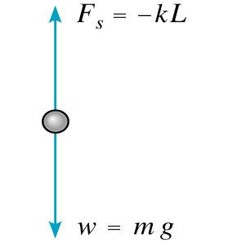
\includegraphics[width=\linewidth]{images/Spring1.jpg}
\end{sbspanel}%
\begin{sbspanel}{0.5}%
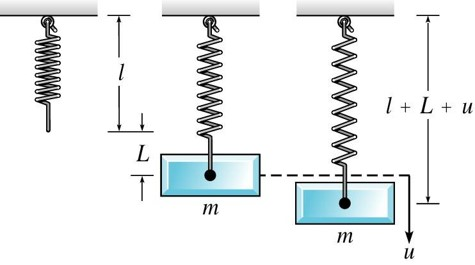
\includegraphics[width=\linewidth]{images/Spring2.jpg}
\end{sbspanel}%
\end{sidebyside}%
%
\par
We will study the motion of a mass when it is acted on by an external force (forcing function) and\slash{}or is initially displaced. Let \(u(t)=\)displacement of the mass from its equilibrium position at time \(t\). The motion of the mass \(u(t)\) is modeled by the following:%
\begin{equation*}
mu^{\prime\prime}(t)+\gamma u^{\prime}(t)+ku(t)=F(t)\,\,\,\,\,\,u(0)=u_{0},u^{\prime}(0)=v_{0}.
\end{equation*}
where \(m,\gamma,k\) are positive.%
\par
The specific constants depend on the measurement system in use. \(m\) is found from \(w=mg\). \(\gamma\) is given in units of \(\frac{\text{weight unit} \cdot s}{\text{distance unit}}\).  \(k\) is found using Hooke's Law, \(mg=kL\).%
\begin{example}{}{g:example:id405375}%
A \(4\) lb mass stretches a spring \(2\) inches. The mass is displaced an additional 6 in. and then released; and is in a medium that exerts a viscous resistance of \(6\) lb when the mass has a velocity of \(3\) ft\slash{}sec. Formulate the IVP that governs the motion of this mass.%
\par
Solution:%
\par
Find \(m\): \(w=mg\) which implies%
\begin{equation*}
m=\frac{w}{g}=\frac{4\text{ lb}}{32\text{ ft/s}^2}=\frac{1}{8}\frac{\text{lb}s^{2}}{ft}
\end{equation*}
%
\par
Find \(\gamma\): Using \(\gamma u^{\prime}=6\) lb we have%
\begin{equation*}
\gamma=\frac{6\text{ lb}}{3\text{ ft/sec}}=2\frac{\text{lb sec}}{\text{ft}}.
\end{equation*}
%
\par
Find \(k\): (Hooke's Law)%
\begin{equation*}
k=\frac{mg}{L}=\frac{4\text{ lb}}{2\text{ in}}=\frac{4\text{ lb}}{(1/6)\text{ ft}}=24\frac{\text{lb}}{ft}.
\end{equation*}
%
\par
Thus%
\begin{equation*}
\frac{1}{8}u^{\prime\prime}+2u^{\prime}+24u=0
\end{equation*}
hence%
\begin{equation*}
u^{\prime\prime}+16u^{\prime}+192u=0,\,\,\,\,u(0)=\frac{1}{2},\,\,\,u^{\prime}(0)=0
\end{equation*}
since \(u(0)=6\text{in }\frac{1\text{ft}}{12\text{in}}=\frac{1}{2}\).%
\par
Solving this%
\begin{equation*}
u(t)=\frac{1}{4}e^{-8t}\left(2\cos\left(8\sqrt{2}t\right)+\sqrt{2}\sin\left(8\sqrt{2}t\right)\right).
\end{equation*}
%
\begin{image}{0}{1}{0}%
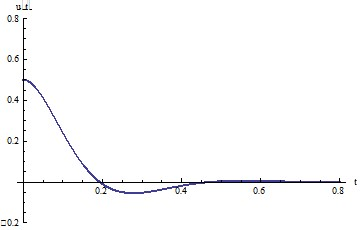
\includegraphics[width=\linewidth]{images/Spring3.jpg}
\end{image}%
\end{example}
\begin{definition}{}{g:definition:id320353}%
When%
\begin{equation*}
u(t)=A\cos\omega_{0}t+B\sin\omega_{0}t=R\cos\left(\omega_{0}t-\delta\right)
\end{equation*}
then \(\omega_{0}=\) is the \terminology{natural frequency} of the system.%
\end{definition}
\end{subsectionptx}
%
%
\typeout{************************************************}
\typeout{Subsection 3.7.2 Derivation of the mass\slash{}spring Differential Equation}
\typeout{************************************************}
%
\begin{subsectionptx}{Derivation of the mass\slash{}spring Differential Equation}{}{Derivation of the mass\slash{}spring Differential Equation}{}{}{g:subsection:id320459}
To see how the differential equation that models the behavior of a mass-spring system is derived, we will recall some basic facts from Physics. Using Newton's Second Law:%
\begin{equation*}
mu^{\prime\prime}(t)=f(t).
\end{equation*}
where \(f\) is the net force acting on the mass.%
\par
The \terminology{forces} are:%
\par
Weight: \(w=mg\) (a downward force).%
\par
Spring force: \(F_{s}=-k\left(L+u(t)\right)\) (either up or down force).%
\par
Damping force: \(F_{d}(t)=-\gamma u^{\prime}(t)\) (either up or down), which may be due to air resistance, friction, machanical device. It acts in the opposite direction as the motion of the mass.%
\par
External force: \(F(t)\) (either an up or down).%
\par
Putting it all together%
\begin{align*}
mu^{\prime\prime}(t) \amp= mg+F_{s}(t)+F_{d}(t)+F(t) \\
\amp= mg-k\left(L+u((t)\right)-\gamma u^{\prime}(t)+F(t)
\end{align*}
which using \(mg=kL\) (from Hooke's Law) and simplifying we have%
\begin{equation*}
mu^{\prime\prime}(t)+\gamma u^{\prime}(t)+ku(t)=F(t)\,\,\,\,\,\,u(0)=u_{0},u^{\prime}(0)=v_{0}.
\end{equation*}
where \(m,\gamma,k\) are positive.%
\end{subsectionptx}
%
%
\typeout{************************************************}
\typeout{Subsection 3.7.3 Undamped harmonic oscillator}
\typeout{************************************************}
%
\begin{subsectionptx}{Undamped harmonic oscillator}{}{Undamped harmonic oscillator}{}{}{g:subsection:id393985}
When the damping coefficient \(\gamma=0\) (nothing stopping it from oscillating forever), we have%
\begin{equation*}
mu^{\prime\prime}+ku=0
\end{equation*}
so that \(mr^{2}+k=0\) gives \(r=\pm i\sqrt{\frac{k}{m}}.\)This is a special number, so we'll denote it \(\omega_{0}=\sqrt{\frac{k}{m}}.\) We get%
\begin{equation*}
u(t)=A\cos\omega_{0}t+B\sin\omega_{0}t
\end{equation*}
with period \(\frac{2\pi}{\omega}\) and the \terminology{natural frequency} of the system is \(\omega_{0}\).%
\end{subsectionptx}
%
%
\typeout{************************************************}
\typeout{Subsection 3.7.4 Damped harmonic oscillator:}
\typeout{************************************************}
%
\begin{subsectionptx}{Damped harmonic oscillator:}{}{Damped harmonic oscillator:}{}{}{g:subsection:id392585}
A \terminology{damper} is an applied force that resists velocity (that is, the damping force is always opposite the direction of motion). A common way to model a damping force is as proportional to the velocity \(u'(t)\). When damped, the model equation becomes%
\begin{equation*}
mu^{\prime\prime}(t)+\gamma u^{\prime}(t)+ku(t)=0.
\end{equation*}
In general we'll have the following characteristic equation%
\begin{equation*}
mr^{2}+\gamma r+k=0,
\end{equation*}
and solving for the roots we get%
\begin{equation*}
r=\frac{-\gamma\pm\sqrt{\gamma^{2}-4km}}{2m}.
\end{equation*}
%
\end{subsectionptx}
%
%
\typeout{************************************************}
\typeout{Subsection 3.7.5 Types of oscillating systems}
\typeout{************************************************}
%
\begin{subsectionptx}{Types of oscillating systems}{}{Types of oscillating systems}{}{}{g:subsection:id392977}
Different types of behavior are possible depending on the value of \(b^{2}-4mk\). We'll classify the possible cases in the following way:%
%
\begin{itemize}[label=\textbullet]
\item{}If \(\gamma=0\),%
\begin{itemize}[label=$\circ$]
\item{}the oscillator is \terminology{undamped}.%
\item{}Mass oscillates forever%
\item{}The natural period is \(2\pi\sqrt{\frac{m}{k}}\).%
\end{itemize}
%
\item{}If \(\gamma>0\) and \(\gamma^{2}-4km\lt0\) (which happens when the roots are \(r=\alpha\pm\beta i\))%
\begin{itemize}[label=$\circ$]
\item{}The oscillator is \terminology{underdamped}. The mass oscillates back and forth as it tends to its rest position. The solutions are%
\begin{equation*}
u=Re^{-\gamma t/(2m)}\cos\left(\mu t-\delta\right)
\end{equation*}
and \(u\) is bounded between \(\pm Re^{-\gamma t/(2m)}\).%
\item{}\begin{image}{0.15}{0.7}{0.15}%
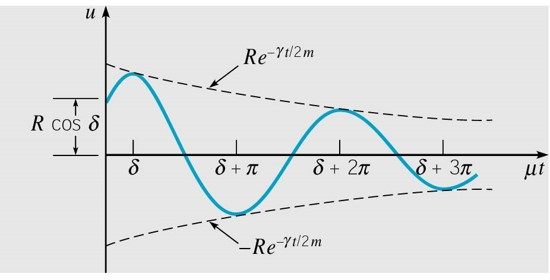
\includegraphics[width=\linewidth]{images/Spring5.jpg}
\end{image}%
%
\end{itemize}
%
\item{}If \(\gamma>0\) and \(\gamma^{2}-4km>0\) (which happens when there are two distinct \(r_{1},r_{2}\)):%
\begin{itemize}[label=$\circ$]
\item{}The oscillator is \terminology{overdamped}. The mass tends to its rest position but does not oscillate.%
\item{}The solutions are%
\begin{equation*}
u=c_{1}e^{r_{1}t}+c_{2}e^{r_{2}t},\,\,\,r_{1},r_{2}\lt0
\end{equation*}
%
\end{itemize}
%
\item{}If \(\gamma>0\) and \(\gamma^{2}-4km=0\) (which happens when there is one negative \(r\)):%
\begin{itemize}[label=$\circ$]
\item{}The oscillator is \terminology{critically damped.} The mass tends to its rest position but does not oscillate.%
\item{}Solutions tend to the origin tangent to the unique line of eigenvectors.%
\item{}The solutions are%
\begin{equation*}
u=c_{1}e^{-\gamma t/(2m)}+c_{2}te^{-\gamma t/(2m)}
\end{equation*}
%
\end{itemize}
%
\end{itemize}
The image below illustrates the behavior possible in different cases. Underdamped is in blue, overdamped in green, and critically damped in red and black.%
\begin{image}{0}{1}{0}%
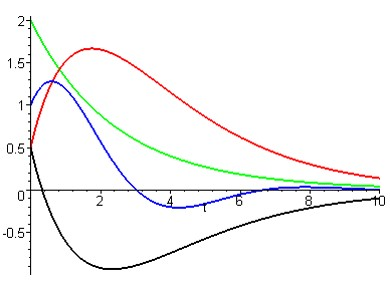
\includegraphics[width=\linewidth]{images/Spring6.jpg}
\end{image}%
\end{subsectionptx}
%
%
\typeout{************************************************}
\typeout{Subsection 3.7.6 Electric Circuts}
\typeout{************************************************}
%
\begin{subsectionptx}{Electric Circuts}{}{Electric Circuts}{}{}{g:subsection:id301815}
The flow of electric charge in certain basic electrical circuits (\terminology{RLC} for resistor (R), inductor (L), capacitor (C)) is modeled by second order linear ODEs with constant coefficients:%
\begin{equation*}
LQ^{\prime\prime}(t)+RQ^{\prime}(t)+\frac{1}{C}Q(t)=E(t),\,\,\,\,\,Q(0)=Q_{0},\,\,\,Q^{\prime}(0)=Q_{0}^{\prime}
\end{equation*}
where \(Q=\) charge (coulombs).%
\begin{image}{0}{1}{0}%
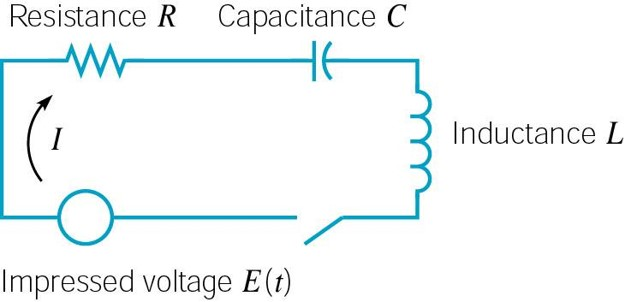
\includegraphics[width=\linewidth]{images/Spring7.jpg}
\end{image}%
\end{subsectionptx}
\end{sectionptx}
%
%
\typeout{************************************************}
\typeout{Section 3.8 Forced oscillations}
\typeout{************************************************}
%
\begin{sectionptx}{Forced oscillations}{}{Forced oscillations}{}{}{x:section:ch3-9}
\begin{introduction}{}%
We consider equations of the form%
\begin{equation*}
mu^{\prime\prime}+\gamma u^{\prime}+ku=F(t)
\end{equation*}
where \(m>0,\gamma>0,k>0\) are mass, damping coefficients, and spring constant. Here \(F(t)\) represents \terminology{external force} done to the mass-spring system. (e.g wind or cars driving on a bridge) While these forcing functions come in many forms, one of the most important cases is where the forcing function is itself a harmonic oscillation (you can think of this as corresponding to an ambient vibration).%
\end{introduction}%
%
%
\typeout{************************************************}
\typeout{Subsection 3.8.1 Harmonic forcing functions}
\typeout{************************************************}
%
\begin{subsectionptx}{Harmonic forcing functions}{}{Harmonic forcing functions}{}{}{g:subsection:id299379}
Suppose that the forcing function is \(F(t)=F_{0}\cos\omega t\), so that the governing equation for the system is%
\begin{equation*}
mu^{\prime\prime}+\gamma u^{\prime}+ku=F(t).
\end{equation*}
Since this is a linear equation in \(u\), recall that we can write the solution as%
\begin{align*}
u(t) \amp =c_{1}u_{1}(t)+c_{2}u_{2}(t)+A\cos\omega t+B\sin\omega t\\
\amp =u_{h}+u_{p},
\end{align*}
and it turns out that \(\lim_{t\to\infty}u_{h}(t)=0\). (See examples above)%
\par
We call \(u_{h}(t)\) a \terminology{transient solution}, as its contribution to the system disappears as time progresses. The particular solution \(u_{p}(t)=A\cos\omega t+B\sin\omega t\) is called the \terminology{steady-state solution}, as it is the long-term, limiting behavior of the system.%
\begin{example}{}{g:example:id299100}%
Consider a undamped harmonic oscillator with model equation%
\begin{equation*}
u^{\prime\prime}+2u=\cos\left(\omega t\right),\,\,\,\,\omega\neq\sqrt{2}.
\end{equation*}
Find the general solution \(u(t)\). What is the natural frequency of the system?%
\par
Solution:%
\par
Step 1: Recall that \(r^{2}+2=0\) so \(r=\pm\sqrt{2}i\), so that%
\begin{equation*}
u_{h}(t)=c_{1}\cos\left(\sqrt{2}t\right)+c_{2}\sin\left(\sqrt{2}t\right).
\end{equation*}
%
\par
Step 2: We make our first guess%
\begin{equation*}
u_{p}(t)=A\cos\left(\omega t\right)+B\sin\left(\omega t\right)
\end{equation*}
and there are no repeats with \(u_{h}\) as long as \(\omega\neq0\), hence we have the correct guess. Thus%
\begin{align*}
u_{p}^{\prime}(t) \amp =-A\omega\sin\left(\omega t\right)+B\omega\cos\left(\omega t\right)\\
u_{p}^{\prime\prime}(t) \amp =-A\omega^{2}\cos\left(\omega t\right)-B\omega^{2}\sin\left(\omega t\right).
\end{align*}
Plugging this into the LHS, we have%
\begin{align*}
LHS=u_{p}^{\prime\prime}+2u_{p} \amp =\left[-A\omega^{2}\cos\left(\omega t\right)-B\omega^{2}\sin\left(\omega t\right)\right]\\
\amp +2A\cos\left(\omega t\right)+2B\sin\left(\omega t\right)\\
\amp =A\left(2-\omega^{2}\right)\cos\left(\omega t\right)+B\left(2-\omega^{2}\right)\sin\left(\omega t\right)
\end{align*}
Then, setting \(LHS=RHS=1\cdot\cos\left(\omega t\right)+0\sin\left(\omega t\right)\) we have%
\begin{align*}
A\left(2-\omega^{2}\right)=1 \amp ,\,\,\,\,\,\,B\left(2-\omega^{2}\right)=0\\
A=\frac{1}{2-\omega^{2}} \amp ,\,\,\,\,\,\,B=0
\end{align*}
so that%
\begin{equation*}
u(t)=c_{1}\cos\left(\sqrt{2}t\right)+c_{2}\sin\left(\sqrt{2}t\right)+\frac{1}{2-\omega^{2}}\cos\left(\omega t\right).
\end{equation*}
%
\end{example}
\end{subsectionptx}
%
%
\typeout{************************************************}
\typeout{Subsection 3.8.2 Resonance (undamped systems)}
\typeout{************************************************}
%
\begin{subsectionptx}{Resonance (undamped systems)}{}{Resonance (undamped systems)}{}{}{g:subsection:id304728}
When the forcing function of an undamped system  is far from the natural frequency of a undamped system, forcing function and the natural behavior of the system interact in a combination of constructive and destructive interference. \leavevmode%
\begin{sageinput}
var('x')
y = function('y')(x)
de = diff(y, x, 2) + 2*y == cos(5*x)
f = desolve(de, y, [0,0,0])
plot(f, [0,10*pi], title = f)
\end{sageinput}
 However, when the frequency of the forcing function approaches the natural frequency of the system, constructive and destructive interference tend to cluster into locally strong or weak oscillations called \terminology{beats}.%
\begin{equation*}
\omega_{0}\approx\omega.
\end{equation*}
Solutions in this case typically look something like this: \begin{image}{0}{1}{0}%
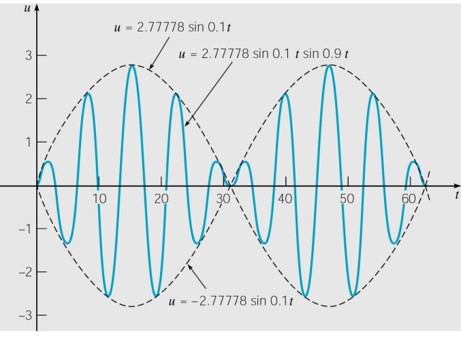
\includegraphics[width=\linewidth]{images/3.8-2.jpg}
\end{image}%
%
\begin{sageinput}
var('x')
y = function('y')(x)
de = diff(y, x, 2) + 2*y == cos(1.21*x)
f = desolve(de, y, [0,0,0])
plot(f, [0,20*pi], title = f)
\end{sageinput}
When the natural and forcing frequencies are equal, the result is \terminology{harmonic resonance}:%
\begin{equation*}
\omega_{0}=\omega.
\end{equation*}
We need a new \(u_{p}\) to solve for when resonance happens, since we can't plug \(\omega=\sqrt{2}\), into \(\frac{1}{2-\omega^{2}}\cos\left(\omega t\right)\). We will see that solution looks like this: \begin{image}{0}{1}{0}%
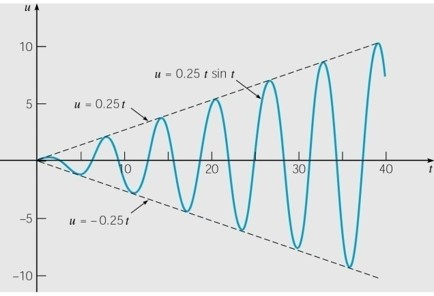
\includegraphics[width=\linewidth]{images/3.8-3.jpg}
\end{image}%
 \begin{sageinput}
var('x')
y = function('y')(x)
de = diff(y, x, 2) + 2*y == cos(sqrt(2)*x)
f = desolve(de, y, [0,0,0])
plot(f, [0,20*pi], title = f)
\end{sageinput}
 That is, the energy of the forcing function is stored in the system with no destructive interference, which results in increasingly wide oscillations. Meaning, if the external forcing and the system oscilations are matching, then the system will become more and more stronger because of the matching external forcing.%
\begin{example}{Resonance.}{g:example:id302754}%
Solve the following undamped harmonic oscillator:%
\begin{equation*}
u^{\prime\prime}+2u=\cos\left(\sqrt{2}t\right),\,\,\,\,u(0)=0,\,\,u^{\prime}(0)=0.
\end{equation*}
What is the natural frequency? What is the frequency for the external force? What kind of behavior of the solution will you get get?%
\par
Solution:%
\par
Step1: Recall that \(r^{2}+2=0\) so \(r=\pm\sqrt{2}i\), so that%
\begin{equation*}
u_{h}(t)=c_{1}\cos\left(\sqrt{2}t\right)+c_{2}\sin\left(\sqrt{2}t\right).
\end{equation*}
The natural frequency of the system is \(\omega_{0}=\sqrt{2}\). The external frequency is \(\omega=\sqrt{2}\). Since they match, then we will get resonance!%
\par
Step 2: We make our first guess%
\begin{equation*}
u_{p}(t)=A\cos\left(\sqrt{2}t\right)+B\sin\left(\sqrt{2}t\right)
\end{equation*}
but we know that this overlaps with the homogeneous solution, so we choose instead our second guess (by multiplying old guess by \(t\))%
\begin{equation*}
u_{p}(t)=At\cos\left(\sqrt{2}t\right)+Bt\sin\left(\sqrt{2}t\right).
\end{equation*}
Then%
\begin{align*}
u_{p}^{\prime}(t) \amp =A\cos\sqrt{2t}-A\sqrt{2}t\sin\sqrt{2}t\\
\amp +B\sin\sqrt{2}t+B\sqrt{2}t\cos\sqrt{2}t\\
u_{p}^{\prime\prime}(t) \amp =-\sqrt{2}A\sin\sqrt{2}t-A\sqrt{2}\sin\sqrt{2}t\\
\amp -A2t\cos\sqrt{2}t\\
\amp B\sqrt{2}\cos\sqrt{2}t+B\sqrt{2}\cos\sqrt{2}t\\
\amp -B2t\sin\sqrt{2}t
\end{align*}
Plugging this into the LHS we have%
\begin{align*}
LHS=u_{p}^{\prime\prime}+2u_{p} \amp =\text{simplify}\\
\amp =2\sqrt{2}B\cos\left(\sqrt{2}t\right)-2\sqrt{2}A\sin\left(\sqrt{2}t\right).
\end{align*}
Now, setting \(LHS=RHS=1\cdot\cos\left(\sqrt{2}t\right)+0\sin\left(\sqrt{2}t\right),\) we have%
\begin{align*}
2\sqrt{2}B=1 \amp ,\,\,\,\,\,\,-2\sqrt{2}A=0\\
B=\frac{1}{2\sqrt{2}} \amp ,\,\,\,\,\,\,A=0
\end{align*}
so that%
\begin{equation*}
u(t)=c_{1}\cos\left(\sqrt{2}t\right)+c_{2}\sin\left(\sqrt{2}t\right)+\frac{1}{2\sqrt{2}}t\sin\left(\sqrt{2}t\right).
\end{equation*}
Using initial condition we have \(c_{1}=0,c_{2}=0\).%
\begin{equation*}
u(t)=\frac{1}{2\sqrt{2}}t\sin\left(\sqrt{2}t\right).
\end{equation*}
Hence we get the picture similar to the one above since%
\begin{equation*}
\frac{1}{2\sqrt{2}}t\sin\left(\sqrt{2}t\right)\approx\pm\frac{t}{2\sqrt{2}}\text{ when }t\text{ is large.}
\end{equation*}
%
\begin{sageinput}
var('x')
y = function('y')(x)
de = diff(y, x, 2) + 2*y == cos(sqrt(2)*x)
f = desolve(de, y, [0,0,0])
plot(f, [0,10*pi], title = f)
\end{sageinput}
\end{example}
\end{subsectionptx}
\end{sectionptx}
%
%
\typeout{************************************************}
\typeout{Section 3.9 Variation of Parameters}
\typeout{************************************************}
%
\begin{sectionptx}{Variation of Parameters}{}{Variation of Parameters}{}{}{x:section:ch3-7}
Consider the equation%
\begin{equation*}
y^{\prime\prime}+4y =\frac{3}{\sin t}
\end{equation*}
MOUC doesn't work with quotients, only products. We will learn a (more complicated) general formula to solving more general linear non-homoheneous 2nd order ODEs. This formula will give a particular solution to a non-homogeneous equation given that you already know what the fundamental set of solutions are for the corresponsing homogeneous equation.%
\begin{theorem}{Variation of Parameters.}{}{x:theorem:thmvarpara}%
If \(p,q,\) and \(g\) are continuous on an open interval \(I\), and if the functions \(\left\{ y_{1},y_{2}\right\} \) form a fundamental set of solutions to the corresponding homogeneous equation%
\begin{equation*}
y^{\prime\prime}+p(t)y^{\prime}+q(t)y=0,
\end{equation*}
then a particular solution to%
\begin{equation*}
y^{\prime\prime}+p(t)y^{\prime}+q(t)y=g(t)
\end{equation*}
is given by%
\begin{align*}
y_{p}(t) \amp =-y_{1}(t)\int_{t_{0}}^{t}\frac{y_{2}(s)g(s)}{W\left(y_{1},y_{2}\right)(s)}ds+y_{2}(t)\int_{t_{0}}^{t}\frac{y_{1}(s)g(s)}{W\left(y_{1},y_{2}\right)(s)}ds\\
\amp =-y_{1}(t)\left[\int\frac{y_{2}(t)g(t)}{W\left(y_{1},y_{2}\right)(t)}dt\right]+y_{2}(t)\left[\int\frac{y_{1}(t)g(t)}{W\left(y_{1},y_{2}\right)(t)}dt\right]
\end{align*}
if the antiderivates exist, where \(t_{0}\) is any value in \(I\). Then the general solution to the non-homogeneous solution is%
\begin{equation*}
y(t)=c_{1}y_{1}(t)+c_{2}y_{2}(t)+y_{p}(t).
\end{equation*}
%
\end{theorem}
\begin{proof}{}{g:proof:id312724}
The proof can be found in any differential equations text, or online. The idea is this: Suppose%
\begin{equation*}
y_{h}(t)=c_{1}y_{1}(t)+c_{2}y_{1}(t)
\end{equation*}
is the general solution to%
\begin{equation*}
y^{\prime\prime}+p(t)y^{\prime}+q(t)y=0.
\end{equation*}
Then the idea is to use the following guess:%
\begin{equation*}
y_{p}(t)=u_{1}(t)y_{1}(t)+u_{2}(t)y_{2}(t)
\end{equation*}
for the non-homogeneous equation, and also make the extra assumption that%
\begin{equation*}
u_{1}^{\prime}(t)y_{1}(t)+u_{2}^{\prime}(t)y_{2}(t)=0.\,\,\,\,\,(\star)
\end{equation*}
The validity of this assumption is difficult to justify without higher level mathematics, but one can at least take comfort in that we have an extra constraint to play with, so for computational convenience we select condition \((\star)\).%
\par
Then take derivatives, simplify and put them back into the differential equation. This will always reduce to%
\begin{align*}
LHS \amp =y_{p}^{\prime\prime}+p(t)y_{p}^{\prime}+q(t)y_{p}\\
\amp =\text{work}\\
\amp =u_{1}^{\prime}y_{1}^{\prime}(t)+u_{2}^{\prime}(t)y_{2}^{\prime}(t)
\end{align*}
and set LHS to RHS which is \(g(t)\) hence we get%
\begin{equation*}
u_{1}^{\prime}(t)y_{1}^{\prime}(t)+u_{2}^{\prime}(t)y_{2}^{\prime}(t)=g(t).\,\,\,\,\,(\star\star)
\end{equation*}
Putting \((\star)\) and \((\star\star)\) together we have the two equations:%
\begin{equation*}
\begin{cases}
u_{1}^{\prime}(t)y_{1}(t)+u_{2}^{\prime}(t)y_{2}(t)=0\\
u_{1}^{\prime}y_{1}^{\prime}(t)+u_{2}^{\prime}(t)y_{2}^{\prime}(t)=g(t)
\end{cases}
\end{equation*}
which boils to solving for \(u_{1}^{\prime}(t)\) and \(u_{2}^{\prime}(t)\) and getting%
\begin{equation*}
\begin{cases}
u_{1}^{\prime}(t)=-\frac{y_{2}(t)g(t)}{W\left(y_{1},y_{2}\right)(t)}\\
u_{2}^{\prime}(t)=\frac{y_{1}(t)g(t)}{W\left(y_{1},y_{2}\right)(t)}
\end{cases}
\end{equation*}
which by integrating we have%
\begin{equation*}
\begin{cases}
u_{1}(t)=-\int\frac{y_{2}(t)g(t)}{W\left(y_{1},y_{2}\right)(t)}dt\\
u_{2}(t)=\int\frac{y_{1}(t)g(t)}{W\left(y_{1},y_{2}\right)(t)}dt
\end{cases}\qedhere
\end{equation*}
%
\end{proof}
\begin{example}{}{g:example:id311211}%
Find a particular solution to%
\begin{equation*}
y^{\prime\prime}+4y=\frac{1}{\cos\left(2t\right)}.
\end{equation*}
%
\par
Step1: First find \(y_{h}\) if possible. In this case \(y_{h}\)will be given by solving \(r^{2}+4=0\) so that \(r=\pm2i\) hence%
\begin{equation*}
y_{h}(t)=c_{1}\cos(2t)+c_{2}\sin\left(2t\right).
\end{equation*}
Thus \(y_{1}(t)=\cos(2t)\) and \(y_{2}(t)=\sin\left(2t\right)\).%
\par
Step2: Find the Wronskian:%
\begin{align*}
W(y_{1},y_{2})(t) \amp =\left|\begin{array}{cc}
\cos(2t) \amp \sin\left(2t\right)\\
-2\sin(2t) \amp 2\cos(2t)
\end{array}\right|\\
\amp =2\cos^{2}(2t)+2\sin^{2}(2t)\\
\amp =2\left[\cos^{2}(2t)+\sin^{2}(2t)\right]\\
\amp =2\cdot1=2.
\end{align*}
%
\par
Step3: Use our formula with \(g(t)=\frac{1}{\cos\left(2t\right)}\) and get%
\begin{align*}
y_{p}(t) \amp =-y_{1}(t)\left[\int\frac{y_{2}(t)g(t)}{W\left(y_{1},y_{2}\right)(t)}dt\right]+y_{2}(t)\left[\int\frac{y_{1}(t)g(t)}{W\left(y_{1},y_{2}\right)(t)}dt\right]\\
\amp =-\cos(2t)\left[\int\frac{1}{2}\frac{\sin(2t)}{\cos\left(2t\right)}dt\right]+\sin(2t)\left[\int\frac{\cos(2t)}{2}\frac{1}{\cos\left(2t\right)}dt\right]\\
\amp =-\cos(2t)\left[\frac{1}{2}\int\frac{\sin(2t)}{\cos\left(2t\right)}dt\right]+\frac{t}{2}\sin(2t)
\end{align*}
%
\par
Now you can remember the antiderivative of \(\int\tan(2t)dt\) or use \(u\)-substitution with \(u=\cos(2t)\) and get \(du=-2\sin(2t)dt\) so that%
\begin{equation*}
\int\frac{\sin(2t)}{\cos\left(2t\right)}dt=-\frac{1}{2}\int\frac{du}{u}=-\frac{1}{2}\ln\left|u\right|=-\frac{1}{2}\ln\left|\cos(2t)\right|
\end{equation*}
hence%
\begin{equation*}
y_{p}(t)=\frac{1}{4}\cos(2t)\ln\left|\cos(2t)\right|+\frac{t}{2}\sin(2t).
\end{equation*}
%
\end{example}
\begin{example}{}{g:example:id309830}%
Find the general solution to%
\begin{equation*}
t^{2}y^{\prime\prime}+2ty^{\prime}-2y=6t
\end{equation*}
given that%
\begin{equation*}
y_{1}(t)=t,\,\,\,y_{2}(t)=t^{-2}
\end{equation*}
forms a fundamental set of solution for the corresponding homogeneous differential equation.%
\par
Step 1: Since \(y_{1}(t)=t,\,\,\,y_{2}(t)=t^{-2}\) forms a fundamental set of solution, this means that the general solution for the homogeneous equation is%
\begin{equation*}
y_{h}=c_{1}t+c_{2}t^{-2}.
\end{equation*}
%
\par
Step 2: Find the Wronskian:%
\begin{align*}
W(y_{1},y_{2})(t) \amp =\left|\begin{array}{cc}
t \amp t^{-2}\\
1 \amp -2t^{-3}
\end{array}\right|\\
\amp =-2t^{-2}-t^{-2}=-3t^{-2}\neq0,
\end{align*}
%
\par
Step 3: Rewrite the equation in the form \(y^{\prime\prime}+p(t)y^{\prime}+q(t)y=g(t)\) and hence%
\begin{equation*}
y^{\prime\prime}+\frac{2}{t}y^{\prime}-\frac{2}{t^{2}}y=\frac{6}{t}.
\end{equation*}
Use our formula with \(g(t)=\frac{6}{t}\) and get%
\begin{align*}
y_{p}(t) \amp =-y_{1}(t)\left[\int\frac{y_{2}(t)g(t)}{W\left(y_{1},y_{2}\right)(t)}dt\right]+y_{2}(t)\left[\int\frac{y_{1}(t)g(t)}{W\left(y_{1},y_{2}\right)(t)}dt\right]\\
\amp =-t\left[\int\frac{t^{-2}}{-3t^{-2}}\frac{6}{t}dt\right]+t^{-2}\left[\int\frac{t}{-3t^{-2})}\frac{6}{t}dt\right]\\
\amp =-t\left[\int\frac{2}{t}dt\right]+t^{-2}\left[\int-2t^{2}dt\right]\\
\amp =-t\left[2\ln t\right]+t^{-2}\left[-\frac{2}{3}t^{3}\right]\\
\amp =-2t\ln t-\frac{2}{3}t.
\end{align*}
Hence, the general solution is%
\begin{align*}
y(t) \amp =y_{h}+y_{p}\\
\amp =c_{1}t+c_{2}t^{-2}-2t\ln t-\frac{2}{3}t.
\end{align*}
%
\end{example}
\begin{example}{}{g:example:id308076}%
Find the general solution to%
\begin{equation*}
t^{2}y^{\prime\prime}-3ty^{\prime}+3y=8t^{3},\,\,\,\,t>0
\end{equation*}
given that%
\begin{equation*}
y_{1}(t)=t,\,\,\,y_{2}(t)=t^{3}
\end{equation*}
forms a fundamental set of solution for the corresponding homogeneous differential equation.%
\par
Step 1: Since \(y_{1}(t)=t,\,\,\,y_{2}(t)=t^{3}\) forms a fundamental set of solution, this means that the general solution for the homogeneous equation is%
\begin{equation*}
y_{h}=c_{1}t+c_{2}t^{3}.
\end{equation*}
%
\par
Step 2: Find the Wronskian:%
\begin{align*}
W(y_{1},y_{2})(t) \amp =\left|\begin{array}{cc}
t \amp t^{3}\\
1 \amp 3t^{2}
\end{array}\right|\\
\amp =3t^{3}-t^{3}=2t^{3}\neq0,
\end{align*}
%
\par
Step 3: Rewrite the equation in the form \(y^{\prime\prime}+p(t)y^{\prime}+q(t)y=g(t)\) and hence%
\begin{equation*}
y^{\prime\prime}-\frac{3}{t}y^{\prime}+\frac{3}{t^{2}}y=8t,.
\end{equation*}
Use our formula with \(g(t)=8t\) and get%
\begin{align*}
y_{p}(t) \amp =-y_{1}(t)\left[\int\frac{y_{2}(t)g(t)}{W\left(y_{1},y_{2}\right)(t)}dt\right]+y_{2}(t)\left[\int\frac{y_{1}(t)g(t)}{W\left(y_{1},y_{2}\right)(t)}dt\right]\\
\amp =-t\left[\int\frac{t^{3}}{2t^{3}}8tdt\right]+t^{3}\left[\int\frac{t}{2t^{3}}8tdt\right]\\
\amp =-t\left[\int4tdt\right]+t^{3}\left[\int\frac{4}{t}dt\right]\\
\amp =-t\left[2t^{2}\right]+t^{3}\left[4\ln t\right]\\
\amp =-2t^{3}+4t^{3}\ln t
\end{align*}
hence the general solution is%
\begin{align*}
y(t) \amp =y_{h}+y_{p}\\
\amp =c_{1}t+c_{2}t^{3}-2t^{3}+4t^{3}\ln t.
\end{align*}
%
\end{example}
\end{sectionptx}
\end{chapterptx}
%
%
\typeout{************************************************}
\typeout{Chapter 4 Higher order differential equations}
\typeout{************************************************}
%
\begin{chapterptx}{Higher order differential equations}{}{Higher order differential equations}{}{}{x:chapter:ch-4}
%
%
\typeout{************************************************}
\typeout{Section 4.1 Linear equations}
\typeout{************************************************}
%
\begin{sectionptx}{Linear equations}{}{Linear equations}{}{}{x:section:ch4-1}
%
%
\typeout{************************************************}
\typeout{Subsection 4.1.1 General linear equations}
\typeout{************************************************}
%
\begin{subsectionptx}{General linear equations}{}{General linear equations}{}{}{g:subsection:id335601}
Everything we did in \hyperref[x:chapter:ch3]{Chapter~{\xreffont\ref{x:chapter:ch3}}}for second order linear equations can be extended to higher order systems. Suppose we have the \(n\)th order linear equation%
\begin{equation*}
a_{n}(t)y^{(n)}+a_{n-1}(t)y^{(n-1)}+\cdots+a_{1}(t)y^{\prime}+a_{0}(t)y=g(t).
\end{equation*}
We assume that \(a_{n}(t),\dots,a_{0}(t)\) are continuous functions on an interval \(I\), and that \(a_{n}(t)\neq0\) inside the interval: so that we can write it in standand form as%
\begin{equation*}
y^{(n)}+p_{n-1}(t)y^{(n-1)}+\cdots+p_{1}(t)y^{\prime}+p_{0}(t)y=g(t).\,\,\,\,\,(\star)
\end{equation*}
with initial conditions%
\begin{equation*}
y(t_{0})=y_{0},\,\,y^{\prime}(t_{0})=y_{0}^{\prime},\,\,\cdots,y^{(n-1)}(t_{0})=y_{0}^{(n-1)}.\,\,\,\,\,(\star)\text{.}
\end{equation*}
%
\begin{theorem}{Existence\slash{}uniqueness.}{}{g:theorem:id336436}%
Let a linear differential equation be given in form \((\star)\). If \(p_{n-1}(t),\dots,p_{0}(t)\) are continuous functions on an open interval \(I\) (containing \(t_{0}\)), then there exists a unique solution \(y=\phi(t)\) throughout all of \(I\) to the IVP in \((\star)\).%
\end{theorem}
\begin{example}{}{g:example:id299762}%
Consider the ODE%
\begin{equation*}
(t-2)y^{(4)}+\sin ty^{\prime\prime\prime}+\ln ty=\sqrt{t+5}.
\end{equation*}
Find the intervals where you are guaranteed a unique solution to this ODE by the Uniqueness and Existence Theorem.%
\par
Rewriting, we have%
\begin{equation*}
y^{(4)}+\frac{\sin t}{(t-2)}y^{\prime\prime\prime}+\frac{\ln t}{(t-2)}y=\frac{\sqrt{t+5}}{(t-2)}
\end{equation*}
and%
\begin{itemize}[label=\textbullet]
\item{}\(\frac{\sin t}{(t-2)}\) is comtinuous when \(t\neq2\)%
\item{}\(\frac{\ln t}{(t-2)}\) is continuous when \(t>0\) and \(t\neq2\), and%
\item{}\(\frac{\sqrt{t+5}}{(t-2)}\) is continuous when \(t\geq-5\) and \(t\neq2\).%
\end{itemize}
Making a number line we see that all three functions are continuous when either on the interval \((0,2)\) or \((2,\infty)\).%
\end{example}
\end{subsectionptx}
%
%
\typeout{************************************************}
\typeout{Subsection 4.1.2 Constant coefficients}
\typeout{************************************************}
%
\begin{subsectionptx}{Constant coefficients}{}{Constant coefficients}{}{}{g:subsection:id303143}
Now consider the homogeneous \(n\)th order linear equation with constant coefficients.%
\begin{equation*}
a_{n}y^{(n)}+a_{n-1}y^{(n-1)}+\cdots+a_{1}y^{\prime}+a_{0}y=0.
\end{equation*}
As we did in the \(2\)nd order case, the first thing we do is guess that the solution will look like \(y=e^{rt}\) and%
\begin{align*}
y \amp =e^{rt}\\
y^{\prime} \amp =re^{rt},\\
\amp \vdots\\
y^{(n)} \amp =r^{n}e^{rt}.
\end{align*}
Plugging into the LHS and setting equal to zero we have%
\begin{align*}
LHS \amp =a_{n}\left(r^{n}e^{rt}\right)+\cdots+a_{1}\left(re^{rt}\right)+a_{0}\left(e^{rt}\right)\\
\amp =e^{rt}\left(a_{n}r^{n}+\cdots+a_{0}\right)\\
\amp =RHS=0
\end{align*}
hence%
\begin{equation*}
e^{rt}\left(a_{n}r^{n}+\cdots+a_{0}\right)=0.
\end{equation*}
But since \(e^{rt}\neq0\) then%
\begin{equation*}
a_{n}r^{n}+\cdots+a_{1}r+a_{0}=0.
\end{equation*}
%
\par
As before the \terminology{characteristic equation} is given by:%
\begin{equation*}
\begin{array}{c}
\underbrace{a_{n}r^{n}+\cdots+a_{0}}\\
Z(r)
\end{array}=0,
\end{equation*}
where we call \(Z(r)\) the characteristic polynomial. How do we solve \(n-\)degree polynomials? By factoring! The fundamental theorem of algebra guarantees that an \(n\)th degree polynomial factors into \(n\) linear terms (assuming that we allow complex roots).%
\begin{equation*}
Z(t)=a_{n}\left(r-r_{1}\right)\left(r-r_{2}\right)\cdots\left(r-r_{n}\right).
\end{equation*}
\alert{HOWEVER}, there is no general approach to factoring polynomials of degree greater than 4. Numerical techniques are necessary in these cases.%
\par
Solutions to the ODE are built exactly like in the 2nd degree case. If there are any repeat solutions, then keep multiplying by \(t\) until you don't have any more repeat solutions.%
\begin{example}{}{g:example:id409742}%
Find general solution and the particular solution to the IVP%
\begin{equation*}
y^{\prime\prime\prime}-2y^{\prime\prime}-y^{\prime}+2y=0.\,\,\,\,y(0)=0,y^{\prime}(0)=1,y^{\prime}(0)=2.
\end{equation*}
(Hint: Suppose you know \(r^{3}-2r^{2}-r+2=\left(r-2\right)\left(r+1\right)\left(r-1\right)\))%
\par
The characteristic equation is \(2r^{3}-4r^{2}-2r+4=0\) and by the hint we have%
\begin{equation*}
\left(r-2\right)\left(r+1\right)\left(r-1\right)=0,
\end{equation*}
hence the general solution is \(y(t)=c_{1}e^{2t}+c_{2}e^{-t}+c_{3}e^{t}\). To find the particular solution to the IVP we start by:%
\begin{align*}
y(t) \amp =c_{1}e^{2t}+c_{2}e^{-t}+c_{3}e^{t}\\
y^{\prime}(t) \amp =2c_{1}e^{2t}-c_{2}e^{-t}+c_{3}e^{t}\\
y^{\prime\prime}(t) \amp =4c_{1}e^{2t}+c_{2}e^{-t}+c_{2}e^{t}.
\end{align*}
Then we have to solve the following system of equations:%
\begin{align*}
0 \amp =c_{1}+c_{2}+c_{3}\\
1 \amp =2c_{1}-c_{2}+c_{3}\\
2 \amp =4c_{1}+c_{2}+c_{3}
\end{align*}
and get \(c_{1}=\frac{2}{3}\), \(c_{2}=-\frac{1}{6}\) and \(c_{3}=-\frac{1}{2}\), hence%
\begin{equation*}
y(t)=\frac{2}{3}e^{2t}-\frac{1}{6}e^{-t}-\frac{1}{2}e^{t}.
\end{equation*}
%
\end{example}
\begin{example}{}{g:example:id517530}%
Find general solution of%
\begin{equation*}
y^{(4)}+8y^{\prime\prime\prime}+16y^{\prime\prime}=0.
\end{equation*}
(Hint: \(r^{4}+8r^{3}+16r^{2}=r^{2}\left(r+4\right)^{2}\))%
\par
The characteristic polynomial is%
\begin{align*}
r^{4}+8r^{3}+16r^{2} \amp =0
\end{align*}
which by the hint we know factors as%
\begin{equation*}
r^{2}\left(r+4\right)^{2}=0.
\end{equation*}
Note that since this a 4th degree polynomial we need to have 4 roots: \(0,0,-4,-4\). So we use the same method we do when we have repeats and get%
\begin{align*}
y(t) \amp =c_{1}e^{0t}+c_{2}te^{0t}+c_{3}e^{-4t}+c_{4}te^{-4t}\\
\amp =c_{1}+c_{2}t+c_{3}e^{-4t}+c_{4}te^{-4t}.
\end{align*}
%
\end{example}
\begin{example}{}{g:example:id517554}%
Solve%
\begin{equation*}
y^{(4)}+y^{\prime\prime\prime}-5y^{\prime\prime}+y^{\prime}-6y=0.
\end{equation*}
(Hint: Suppose \(\left(r-2\right)\left(r+3\right)\left(r^{2}+1\right)\))%
\par
The characteristic equation is given by%
\begin{equation*}
r^{4}+r^{3}-5r^{2}+r-6=0
\end{equation*}
and by the hint%
\begin{equation*}
Z(r)=\left(r-2\right)\left(r+3\right)\left(r^{2}+1\right)=0
\end{equation*}
which gives%
\begin{equation*}
r=2,-3,\pm i
\end{equation*}
hence%
\begin{equation*}
y(t)=c_{1}e^{2t}+c_{2}e^{-3t}+c_{3}\cos t+c_{3}\sin t.
\end{equation*}
%
\end{example}
\begin{example}{}{g:example:id517570}%
Solve%
\begin{equation*}
y^{\prime\prime\prime}-3y^{\prime\prime}+3y^{\prime}-y=0.
\end{equation*}
(Hint: \(r^{3}-3r^{2}+3r-1=\left(r-1\right)\left(r-1\right)^{2}\))%
\par
The characteristic polynomial is \(r^{3}-3r^{2}+3r-1=0\) and by the hint,%
\begin{equation*}
\left(r-1\right)^{3}=0
\end{equation*}
\textbackslash{}item So that \(r=1,1,1\)%
\begin{equation*}
y(t)=c_{1}e^{t}+c_{2}te^{t}+c_{3}t^{2}e^{t}.
\end{equation*}
%
\end{example}
\begin{example}{}{g:example:id517596}%
Solve%
\begin{equation*}
y^{(4)}+8y^{\prime\prime}-9y=0
\end{equation*}
(Hint: \(r^{4}+8r^{2}-9=\left(r^{2}-1\right)\left(r^{2}+9\right)\))%
\par
By the hint%
\begin{align*}
r^{4}+8r^{2}-9 \amp =\left(r^{2}-1\right)\left(r^{2}+9\right)\\
\amp =\left(r-1\right)\left(r+1\right)\left(r-3i\right)\left(r+3i\right).
\end{align*}
then%
\begin{equation*}
y(t)=c_{1}e^{t}+c_{2}e^{-t}+c_{3}\cos(3t)+c_{4}\sin(3t).
\end{equation*}
%
\end{example}
\begin{example}{}{g:example:id517644}%
Suppose the roots of the characteristic equation are%
\begin{equation*}
2,3,3,3,2\pm3i,2\pm3i
\end{equation*}
then the general solution is%
\begin{align*}
y(t) \amp =c_{1}e^{2t}+c_{2}e^{3t}+c_{3}te^{3t}+c_{4}t^{2}e^{3t}\\
\amp +c_{5}e^{2t}\cos(3t)+c_{6}e^{2t}\sin(3t)\\
\amp +c_{5}te^{2t}\cos(3t)+c_{6}te^{2t}\sin(3t).
\end{align*}
%
\end{example}
\end{subsectionptx}
\end{sectionptx}
%
%
\typeout{************************************************}
\typeout{Section 4.2 The Method of Undetermined Coefficients}
\typeout{************************************************}
%
\begin{sectionptx}{The Method of Undetermined Coefficients}{}{The Method of Undetermined Coefficients}{}{}{x:section:ch4-2}
We consider%
\begin{equation*}
y^{(n)}+p_{n-1}(t)y^{(n-1)}+\cdots+p_{1}(t)y^{\prime}+p_{0}(t)y=g(t)
\end{equation*}
where \(g(t)\) can be a polynomial, sin, cos, exp or products of these. Recall the general solution is of the form: \(y=y_{h}+y_{p}\) where \(y_{h}\) is the general solution of the corresponding homogeneous equation and \(y_{p}\) is a particular solution to the non-homogeneous equation.%
\begin{example}{}{g:example:id517678}%
Find the general solution of%
\begin{equation*}
y^{\prime\prime\prime}-y^{\prime\prime}-y^{\prime}+y=2e^{-t}+3.
\end{equation*}
(Hint: \(r^{3}-r^{2}-r+1=\left(r-1\right)\left(r-1\right)\left(r+1\right)\))%
\par
Step 1: We find \(y_{h}\): Solve \(r^{3}-r^{2}-r+1=0\), but by the hint%
\begin{equation*}
\left(r-1\right)\left(r-1\right)\left(r+1\right)=0
\end{equation*}
so that \(y_{h}=c_{1}e^{t}+c_{2}te^{t}+c_{3}e^{-t}\).%
\par
Step 2: Find \(y_{p}\): We first guess \(y_{p}=Ae^{-t}+B\), but there are repeats with \(y_{h}\) hence we get a second guess of%
\begin{align*}
y_{p} \amp =Ate^{-t}+B\\
y_{p}^{\prime} \amp =Ae^{-t}-Ate^{-t}\\
y_{p}^{\prime\prime} \amp =-Ae^{-t}-Ae^{-t}+Ate^{-t}=-2Ae^{-t}+Ate^{-t}\\
y_{p}^{\prime\prime\prime} \amp =2Ae^{-t}+Ae^{-t}-Ate^{-t}=3Ae^{-t}-Ate^{-t}
\end{align*}
Hence%
\begin{align*}
LHS \amp =3Ae^{-t}-Ate^{-t}\\
\amp +2Ae^{-t}-Ate^{-t}\\
\amp -Ae^{-t}+Ate^{-t}\\
\amp +Ate^{-t}+B\\
\amp =4Ae^{-t}+B
\end{align*}
%
\par
Step 3: Set LHS=RHS so that%
\begin{equation*}
LHS=4Ae^{-t}+B=2e^{-t}+3=RHS
\end{equation*}
hence%
\begin{align*}
4A=2 \amp ,B=3\\
A=\frac{1}{2}
\end{align*}
hence%
\begin{equation*}
y_{p}=\frac{1}{2}te^{-t}+3
\end{equation*}
so that the General Solution is%
\begin{equation*}
y=c_{1}e^{t}+c_{2}te^{t}+c_{3}e^{-t}+\frac{1}{2}te^{-t}+3.
\end{equation*}
%
\end{example}
\begin{example}{}{g:example:id517755}%
Consider%
\begin{equation*}
y^{\prime\prime\prime}+4y^{\prime}=t+\sin(4t).
\end{equation*}
Find the general form of \(y_{p}\).%
\par
Step 1: We find \(y_{h}\): Solve%
\begin{align*}
r^{3}+4r \amp =0\\
r\left(r^{2}+4\right) \amp =0
\end{align*}
so that \(y_{h}=c_{1}+c_{2}\cos2t+c_{3}\sin2t\).%
\par
Step 2: Find \(y_{p}\): We first guess \(y_{p}=At+B+C\cos(4t)+D\sin(4t)\). But \(B\) is already in \(y_{c}\) as \(c_{1}\). So instead make the second guess \(y_{p}=t\left(At+B\right)+C\cos(4t)+D\sin(4t)\) which is correct.%
\end{example}
\begin{example}{}{g:example:id517827}%
Consider%
\begin{equation*}
y^{(4)}-2y^{\prime\prime}+y=e^{t}+te^{-t}.
\end{equation*}
Find the general form of \(y_{p}\). (Hint: \(r^{4}-2r^{2}+1=\left(r^{2}-1\right)^{2}\))%
\par
Step 1: We find \(y_{h}\): Solve%
\begin{align*}
r^{4}-2r^{2}+1 \amp =0\\
\left(r^{2}-1\right)^{2} \amp =0
\end{align*}
so that \(y_{h}=c_{1}e^{t}+c_{2}te^{t}+c_{3}e^{-t}+c_{4}te^{-t}\).%
\par
Step 2: Find \(y_{p}\):%
\begin{enumerate}
\item{}First guess: \(y_{p}=Ae^{t}+\left(Bt+C\right)e^{-t}\).%
\item{}Second Guess: \(y_{p}=Ate^{t}+\left(Bt^{2}+Ct\right)e^{-t}\).%
\item{}Third Guess: \(y_{p}=At^{2}e^{t}+\left(Bt^{3}+Ct^{2}\right)e^{-t}\).%
\end{enumerate}
%
\end{example}
\begin{example}{}{g:example:id517862}%
Suppose%
\begin{equation*}
y^{(5)}=t^{3},
\end{equation*}
find the general form for \(y_{p}\).%
\par
We find \(y_{h}\): The roots to \(r^{5}=0\) are%
\begin{equation*}
r=0,0,0,0,0
\end{equation*}
so that%
\begin{equation*}
y_{c} =c_{1}+c_{2}t+c_{3}t^{2}+c_{4}t^{3}+c_{4}t^{4}
\end{equation*}
%
\par
Step 2: Find \(y_{p}\):%
\begin{enumerate}
\item{}First Guess: \(y_{p}=At^{3}+Bt^{2}+Ct+D\)%
\item{}Final Guess:\textbraceright{}\textbraceright{} \(y_{p}=t^{5}\left(At^{3}+Bt^{2}+Ct+D\right)\)%
\end{enumerate}
%
\end{example}
\end{sectionptx}
\end{chapterptx}
%
%
\typeout{************************************************}
\typeout{Chapter 5 Systems of First Order Linear Equations}
\typeout{************************************************}
%
\begin{chapterptx}{Systems of First Order Linear Equations}{}{Systems of First Order Linear Equations}{}{}{x:chapter:ch5}
%
%
\typeout{************************************************}
\typeout{Section 5.1 Systems of First Order Linear Equations}
\typeout{************************************************}
%
\begin{sectionptx}{Systems of First Order Linear Equations}{}{Systems of First Order Linear Equations}{}{}{x:section:ch5-1}
\begin{introduction}{}%
We start by giving some examples of systems of differential equations with 2 unknown functions.%
\end{introduction}%
%
%
\typeout{************************************************}
\typeout{Subsection 5.1.1 Predator-Prey system}
\typeout{************************************************}
%
\begin{subsectionptx}{Predator-Prey system}{}{Predator-Prey system}{}{}{g:subsection:id517956}
Let \(R(t)=\) prey population and let \(F(t)=\) predator population. Then the following is a system of first order equations:%
\begin{align*}
\frac{dR}{dt} \amp = 2R-1.2RF\\
\frac{dF}{dt}  \amp = -F+0.9RF.
\end{align*}
Notice that the prey and predator population are dependent on each other, and thus we need a system of equations. For example, if there are too many predators then normally that would decrease the population of the prey.%
\end{subsectionptx}
%
%
\typeout{************************************************}
\typeout{Subsection 5.1.2 Spring-Mass Systems and Mixing Problems}
\typeout{************************************************}
%
\begin{subsectionptx}{Spring-Mass Systems and Mixing Problems}{}{Spring-Mass Systems and Mixing Problems}{}{}{g:subsection:id517954}
Suppose we have mass attached to a spring which is attached to another mass attached to a another spring. The behavior of one mass is affected by the other (and vice versa). We need a system of ODE to solve such problems.%
\par
Suppose we have one tank that is being mixed with a solution that flows into another tank. We need systems of equations to determine the amount of mass in each tank.%
\begin{example}{Double Tank Problem.}{g:example:id517944}%
Salt water with concentration \(3\) g\slash{}L of salt flows into tank \#1 at a rate \(4\) L\slash{}min. at a rate of \(4\) L\slash{}min.%
\begin{itemize}[label=\textbullet]
\item{}The well mixed mixture from tank \#1 flows into tank \#2 at a rate of 4 L\slash{}min, and the well mixed mixture of tank \#2 flows out at a rate of 4 L\slash{}min.%
\item{}Tank \#1 initially has 30 L of salt water with \(6\) g of salt dissolved in it.%
\item{}Tank \#2 initially has 20 L of fresh water.%
\end{itemize}
\terminology{Question:} Write a system of ODEs representing this problem. \terminology{Solution:}%
\par
Step 1: First we define variables.%
\par
Let \(x_{1}(t)\) and \(x_{2}(t)\)  be the amount of salt in tank \#1 and tank \#2, respectively at time \(t \)  (minutes).%
\par
Step 2: Use \(x_{i}^{\prime}=\text{Rate in }-\text{Rate out}\).%
\par
We first get%
\begin{align*}
x_{1}^{\prime}(t)  \amp =\left(\text{concentration in}\right)\times\text{Rate}-\left(\text{concentration out}\right)\times\text{Rate}   \\
\amp =3\frac{\text{g}}{L}\cdot4\frac{\text{L}}{\text{min}}-\frac{x_{1}(t)}{\text{water in tank 1 at time t}}\cdot 4\frac{\text{L}}{\text{min}}
\end{align*}
but since%
\begin{equation*}
\text{water at time }t=30+\left(4-4\right)t=30
\end{equation*}
hence%
\begin{equation*}
x_{1}^{\prime}(t) =12-\frac{4x_{1}(t)}{30},x_{1}(0)=6.
\end{equation*}
%
\par
Step 3: Use \(x_{i}^{\prime}=\text{Rate in }-\text{Rate out}\). We first get%
\begin{align*}
x_{2}^{\prime}(t)  \amp =\left(\begin{array}{c}
\mbox{concentration}\\
\mbox{of salt coming in}
\end{array}\right)\times\mbox{Rate}-\left(\begin{array}{c}
\mbox{concentration}\\
\mbox{of salt coming out}
\end{array}\right)\times\mbox{Rate}  \\
\amp =\frac{x_{1}(t)}{30}\frac{\text{g}}{L}\cdot4\frac{\text{L}}{\text{min}}-\frac{x_{2}(t)}{20+(4-4)t}\cdot4\frac{\text{L}}{\text{min}}\\
\amp =\frac{4x_{1}(t)}{30}-\frac{4x_{2}(t)}{20},\,\,\,\,\,x_{2}(0)=0
\end{align*}
Putting it together, the system we have is%
\begin{equation*}
\begin{cases}
x_{1}^{\prime}=12-\frac{2}{15}x_{1} \amp x_{1}(0)=6.\\
x_{2}^{\prime}=\frac{4}{30}x_{1}-\frac{1}{5}x_{2} \amp x_{2}(0)=0
\end{cases}
\end{equation*}
%
\end{example}
\end{subsectionptx}
%
%
\typeout{************************************************}
\typeout{Subsection 5.1.3 Overview of system of ODEs}
\typeout{************************************************}
%
\begin{subsectionptx}{Overview of system of ODEs}{}{Overview of system of ODEs}{}{}{g:subsection:id518074}
We will be dealing only with \(2\times2\) systems, or sometimes \(3\times3\) systems. But in general we can have \(n\times n\) systems. The following is called a \terminology{linear homogeneous system} of \terminology{First Order Equations}:%
\begin{align*}
x_{1}^{\prime} \amp =a(t)x_{1}+b(t)x_{2}\\
x_{2}^{\prime} \amp =c(t)x_{1}+d(t)x_{2}
\end{align*}
The following system is called \terminology{non-homogeneous} if%
\begin{align*}
x_{1}^{\prime} \amp =a(t)x_{1}+b(t)x_{2}+g_{1}(t)\\
x_{2}^{\prime} \amp =c(t)x_{1}+d(t)x_{2}+g_{2}(t)
\end{align*}
where \(g_{1}(t)\) or \(g_{2}(t)\neq 0\).%
\par
An \terminology{initial value problem (IVP)} consists of a system of differential equations and intial conditions such as%
\begin{equation*}
\begin{cases}
x_{1}^{\prime}=a(t)x_{1}+b(t)x_{2} \amp x_{1}(t_{0})=x_{1}^{0}\\
x_{2}^{\prime}=c(t)x_{1}+d(t)x_{2} \amp x_{2}(t_{0})=x_{2}^{0}
\end{cases}
\end{equation*}
%
\par
\terminology{Existence\slash{}Uniqueness?} As long as all the coefficient functions are all continuous then we have the existence and uniqueness of a solution \(\left(x_{1}(t),x_{2}(t)\right) \) to any IVP.%
\end{subsectionptx}
%
%
\typeout{************************************************}
\typeout{Subsection 5.1.4 Turning a Second Order ODE into a System of First Order of ODEs}
\typeout{************************************************}
%
\begin{subsectionptx}{Turning a Second Order ODE into a System of First Order of ODEs}{}{Turning a Second Order ODE into a System of First Order of ODEs}{}{}{g:subsection:id518122}
If we would like to turn a Second Order Linear ODE into a system of equations, the trick is to let%
\begin{equation*}
x_{1}=y,x_{2}=y^{\prime}.
\end{equation*}
%
\begin{example}{Turning an ODE into a system.}{g:example:id518127}%
Turn%
\begin{equation*}
y^{\prime\prime}+\frac{1}{2}y^{\prime}+2y=\sin t
\end{equation*}
into a system of differential equations.%
\par
\terminology{Solution:}%
\par
Goal:  We let \(x_{1}=y\) , \(x_{2}=y^{\prime}\) and set up the following system:%
\begin{align*}
x_{1}^{\prime} \amp =?\\
x_{2}^{\prime} \amp =? 
\end{align*}
%
\par
To do so, we start with what we defined and take derivatives:%
\begin{equation*}
\begin{array}{ccc}
x_{1}=y \amp \implies \amp x_{1}^{\prime}=y^{\prime}=x_{2}\\
x_{2}=y^{\prime} \amp \implies \amp  x_{2}^{\prime}=y^{\prime\prime}=-\frac{1}{2}y^{\prime}-2y-\sin t
\end{array}
\end{equation*}
hence%
\begin{align*}
x_{2}^{\prime} \amp =-\frac{1}{2}y^{\prime}-2y-\sin t \\
\amp =-\frac{1}{2}x_{2}-2x_{1}-\sin t,\text{ by definition} 
\end{align*}
thus%
\begin{equation*}
\begin{cases}
x_{1}^{\prime}=x_{2}\\
x_{2}^{\prime}=-2x_{1}-\frac{1}{2}x_{2}+\sin t
\end{cases}
\end{equation*}
%
\end{example}
\begin{assemblage}{Turning any Second Order Linear ODE into Systems of First Order ODEs.}{g:assemblage:id518164}%
If we have%
\begin{equation*}
a(t)y^{\prime\prime}+b(t)y^{\prime}+c(t)y=g(t)
\end{equation*}
then we by letting \(x_{1}=y\) and \(x_{2}=y^{\prime}\), and using the method in the above example, we can obtain%
\begin{equation*}
\begin{cases}
x_{1}^{\prime}=x_{2}\\
x_{2}^{\prime}=-\frac{c}{a}x_{1}-\frac{b}{a}x_{2}+\frac{g}{a}
\end{cases}
\end{equation*}
%
\end{assemblage}
\end{subsectionptx}
\end{sectionptx}
%
%
\typeout{************************************************}
\typeout{Section 5.2 Review of Matrices, Vector Fields, Phase Planes and Portraits}
\typeout{************************************************}
%
\begin{sectionptx}{Review of Matrices, Vector Fields, Phase Planes and Portraits}{}{Review of Matrices, Vector Fields, Phase Planes and Portraits}{}{}{x:section:ch5-2}
\begin{introduction}{}%
We will start by considering the following \terminology{linear system with constant coefficients}:%
\begin{align*}
x_{1}^{\prime} \amp =  ax_{1}+bx_{2}\\
x_{2}^{\prime} \amp =  cx_{1}+dx_{2}.
\end{align*}
Let%
\begin{equation*}
A=\left(\begin{array}{cc}
a \amp b\\
c \amp d
\end{array}\right)
\end{equation*}
be a matrix and let \(\mathbf{x}=\left(\begin{array}{c}
x_{1}\\
x_{2}
\end{array}\right)\) be a vector. We can define \terminology{matrix-vector} product as%
\begin{equation*}
A\mathbf{x}=\left(\begin{array}{cc}
a \amp b\\
c \amp d
\end{array}\right)\left(\begin{array}{c}
x_{1}\\
x_{2}
\end{array}\right)=\left(\begin{array}{c}
ax_{1}+bx_{2}\\
cx_{1}+dx_{2}
\end{array}\right).
\end{equation*}
For example, if \(A=\left(\begin{array}{cc}
1 \amp 2\\
-1 \amp 3
\end{array}\right)\) and \(\mathbf{x}=\left(\begin{array}{c}
2\\
1
\end{array}\right)\), then%
\begin{equation*}
A\mathbf{x}=\left(\begin{array}{cc}
1 \amp 2\\
-1 \amp 3
\end{array}\right)\left(\begin{array}{c}
2\\
1
\end{array}\right)=\left(\begin{array}{c}
2+2\\
-2+3
\end{array}\right)=\left(\begin{array}{c}
4\\
1
\end{array}\right)
\end{equation*}
One can also \terminology{add} vectors and \terminology{scale} vectors! For example, if \(\mathbf{x}_{1}=\left(\begin{array}{c}
x_{1}\\
x_{2}
\end{array}\right)\) and \(\mathbf{x}_{2}=\left(\begin{array}{c}
y_{1}\\
y_{2}
\end{array}\right)\), then%
\begin{equation*}
\mathbf{x}_{1}+\mathbf{x}_{2}=\left(\begin{array}{c}
x_{1}+y_{1}\\
x_{1}+y_{2}
\end{array}\right)
\end{equation*}
and if \(c\in\mathbb{R}\) then%
\begin{equation*}
c\mathbf{x}_{1}=c\left(\begin{array}{c}
x_{1}\\
x_{2}
\end{array}\right)=\left(\begin{array}{c}
cx_{1}\\
cx_{2}
\end{array}\right)
\end{equation*}
%
\par
Thus we can write a system of ODES, such as%
\begin{align*}
x_{1}^{\prime} \amp =  ax_{1}+bx_{2}\\
x_{2}^{\prime} \amp =  cx_{1}+dx_{2}.
\end{align*}
as%
\begin{equation*}
\mathbf{x}^{\prime}=A\mathbf{x}
\end{equation*}
where \(A=\left(\begin{array}{cc}
a \amp b\\
c \amp d
\end{array}\right)\) and \(\mathbf{x}=\left(\begin{array}{c}
x_{1}\\
x_{2}
\end{array}\right)\). Here \(A\) is called the coefficient matrix. One could also write%
\begin{equation*}
\frac{d\mathbf{x}}{dt}=A\mathbf{x}.
\end{equation*}
%
\end{introduction}%
\begin{example}{}{g:example:id518281}%
The system%
\begin{align*}
x_{1}^{\prime} \amp =-2x_{1}+x_{2}\\
x_{2}^{\prime} \amp =x_{1}-2x_{2}
\end{align*}
can be represented by%
\begin{align*}
\left(\begin{array}{c}
x_{1}^{\prime}\\
x_{2}
\end{array}\right) \amp =\left(\begin{array}{cc}
-2 \amp 1\\
1 \amp -2
\end{array}\right)\left(\begin{array}{c}
x_{1}\\
x_{2}
\end{array}\right) \\
\mathbf{x}^{\prime} \amp =A\mathbf{x}
\end{align*}
%
\end{example}
\begin{example}{}{g:example:id518344}%
Verify that \(\mathbf{x}=\left(\begin{array}{c}
1\\
-2
\end{array}\right)e^{-4t}\) is a solution to%
\begin{equation*}
\mathbf{x}^{\prime}=\left(\begin{array}{cc}
2 \amp 3\\
4 \amp -2
\end{array}\right)\mathbf{x}.
\end{equation*}
%
\par
\terminology{Solution:}%
\par
We plug \(\mathbf{x}=\left(\begin{array}{c}
1\\
-2
\end{array}\right)e^{-4t}\) into the LHS and RHS and see if they are equal to each other%
\begin{equation*}
\text{LHS}=\mathbf{x}^{\prime}=\left(\begin{array}{c}
e^{-4t}\\
-2e^{-4t}
\end{array}\right)^{\prime}=\left(\begin{array}{c}
-4e^{-4t}\\
8e^{-4t}
\end{array}\right)
\end{equation*}
and%
\begin{align*}
\text{RHS} \amp =\left(\begin{array}{cc}
2 \amp 3\\
4 \amp -2
\end{array}\right)\mathbf{x}=\left(\begin{array}{cc}
2 \amp 3\\
4 \amp -2
\end{array}\right)\left(\begin{array}{c}
e^{-4t}\\
-2e^{-4t}
\end{array}\right)\\
\amp =\left(\begin{array}{c}
2e^{-4t}-6e^{-4t}\\
4e^{-4t}+4e^{-4t}
\end{array}\right)\\
\amp =\left(\begin{array}{c}
-4e^{-4t}\\
8e^{-4t}
\end{array}\right)
\end{align*}
since%
\begin{equation*}
\text{LHS}=\text{RHS}
\end{equation*}
then \(\mathbf{x}=\left(\begin{array}{c}
1\\
-2
\end{array}\right)e^{-4t}\) is a solution to this system.%
\end{example}
%
%
\typeout{************************************************}
\typeout{Subsection 5.2.1 Visualizing solutions to systems of first order ODEs (Phase Planes\slash{}Phase Portraits)}
\typeout{************************************************}
%
\begin{subsectionptx}{Visualizing solutions to systems of first order ODEs (Phase Planes\slash{}Phase Portraits)}{}{Visualizing solutions to systems of first order ODEs (Phase Planes\slash{}Phase Portraits)}{}{}{g:subsection:id518362}
What do solutions \(\mathbf{x}(t)\) to \(\mathbf{x}^{\prime}=A\mathbf{x}\) look like? \terminology{They are parametric equations in the plane!}. We can graph in the \(x_{1}-x_{2}\) plane since%
\begin{equation*}
\mathbf{x}(t)=\left(x_{1}(t),x_{2}(t)\right)
\end{equation*}
is a vector (or point) that changes in time. Recall that this requires some knowledge of multivariable Calculus. Also note that there is no axis for time here! Imagine a curve passing through time.%
\par
The \terminology{Phase Plane} is  the \(x_1-x_2\) plane in which the parametric curve (or trajectory) of the solution \(\mathbf{x}(t)=\left(x_{1}(t),x_{2}(t)\right)\) is drawn.%
\begin{example}{}{g:example:id518421}%
Suppose \(\mathbf{x}(t)=\left(\cos t,\sin t\right)\), draw the trajectory of \(\mathbf{x}(t) \) for \(0\leq t\leq2\pi\) on the Phase plane. \begin{image}{0}{1}{0}%
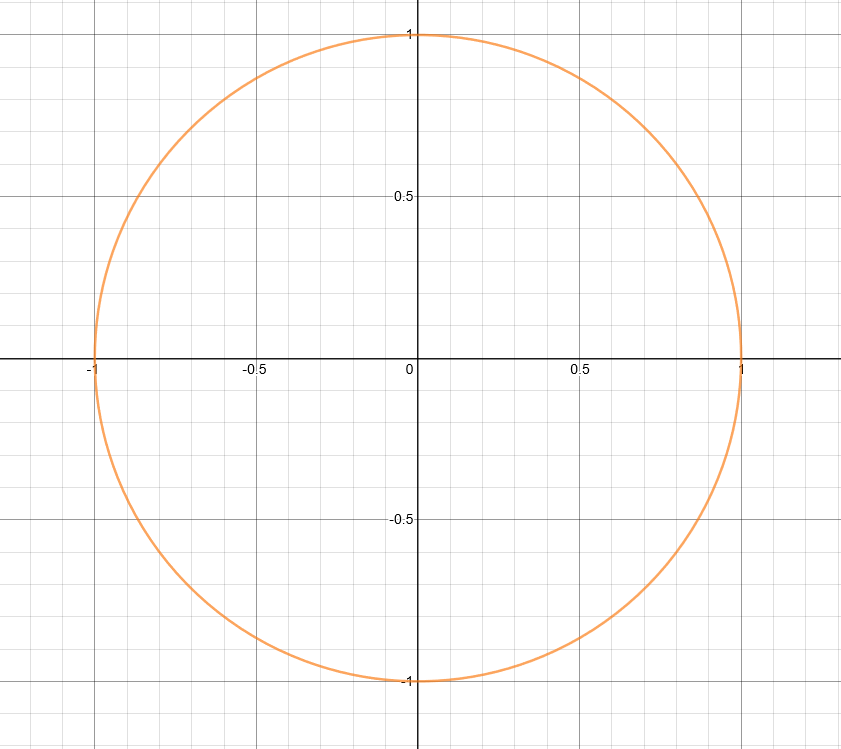
\includegraphics[width=\linewidth]{images/5-parametric1.png}
\end{image}%
%
\end{example}
A \terminology{Phase Portrait}  is a portrait of several different solutions to the system with different initial conditions conditions.%
\begin{example}{}{g:example:id518407}%
Here is an example of a Phase Portrait drawn on the Phase plane. \begin{image}{0}{1}{0}%
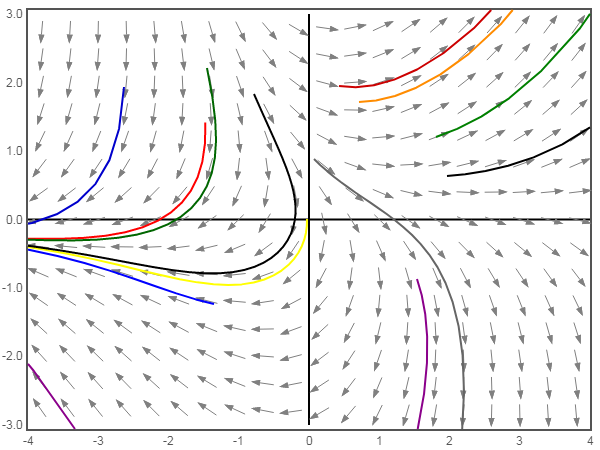
\includegraphics[width=\linewidth]{images/7.2-1.png}
\end{image}%
%
\end{example}
What are the simplest solutions? An \terminology{equilibrium solution} is a constant solution: \(\mathbf{x}(t)=(x_{0},y_{0})\). An equilibrum solution is graphed as dot, since as time moves on, the vector stays constant in the same place. To solve for the equilibrium solution you set the derivatives equal to zero, in this case%
\begin{equation*}
A\mathbf{x}=\mathbf{0}.
\end{equation*}
%
\begin{example}{}{g:example:id518456}%
Find the Equilibrium solutions to%
\begin{equation*}
\mathbf{x}^{\prime}=\left(\begin{array}{cc}
1 \amp 2\\
2 \amp 4
\end{array}\right)\mathbf{x}
\end{equation*}
We must solve%
\begin{align*}
\left(\begin{array}{cc}
1 \amp 2\\
2 \amp 4
\end{array}\right)\mathbf{x}=0 \amp \iff\begin{cases}
x_{1}+2x_{2}=0\\
2x_{1}+4x_{2}=0
\end{cases}\\
\amp \iff x_{1}=-2x_{2}
\end{align*}
since these equations are multiple of each other than there is a whole line of solutions:%
\begin{equation*}
x_{1}=-2x_{2}
\end{equation*}
and it turn out that the solution are of then form:%
\begin{align*}
\mathbf{x}(t) \amp =\left(\begin{array}{c}
-2x_{2}\\
x_{2}
\end{array}\right)\\
\amp =x_{2}\left(\begin{array}{c}
-2\\
1
\end{array}\right).
\end{align*}
Using a generic constant \(c \), we have that there are an infinite number of equilibrium solutions:%
\begin{equation*}
\mathbf{x}(t)=c\left(\begin{array}{c}
-2\\
1
\end{array}\right).
\end{equation*}
%
\end{example}
\begin{example}{}{g:example:id518492}%
Find the Equilibrium solutions to%
\begin{equation*}
\mathbf{x}^{\prime}=\left(\begin{array}{cc}
1 \amp 2\\
3 \amp 4
\end{array}\right)\mathbf{x}
\end{equation*}
We must solve%
\begin{align*}
\left(\begin{array}{cc}
1 \amp 2\\
3 \amp 4
\end{array}\right)\mathbf{x}=0 \amp \iff\begin{cases}
x_{1}+2x_{2}=0\\
3x_{1}+4x_{2}=0
\end{cases}\\
\amp \iff x_{1}=0, x_{2}=0
\end{align*}
%
\end{example}
A \terminology{vector field} is an assignment of a vector to each point in the plane.  We consider vector fields  of the system%
\begin{equation*}
\mathbf{x}^{\prime}=A\mathbf{x}
\end{equation*}
which can be drawn using the following assignment:%
\begin{equation*}
\mathbf{F}(x_{1},x_{2})=A\mathbf{x}.
\end{equation*}
%
\par
Or more generally, if the system is written as%
\begin{equation*}
\begin{cases}
x_{1}^{\prime}=f(x_{1},x_{2})\\
x_{2}=g(x_{1},x_{2})
\end{cases}
\end{equation*}
then we can rewrite this as%
\begin{equation*}
\mathbf{x}^{\prime}=\mathbf{F}\left(\mathbf{x}\right)
\end{equation*}
where the vector field on the right hand side is given by%
\begin{equation*}
\mathbf{F}\left(\mathbf{x}\right)=\mathbf{F}\left(x_{1},x_{2}\right)=\left(\begin{array}{c}
f(x_{1},x_{2})\\
g(x_{1},x_{2})
\end{array}\right).
\end{equation*}
Note if we picture \(\mathbf{x}(t)\) as particle moving through space, then \(\mathbf{x}^{\prime}\) represents the vector tangent to the curve drawn out by \(\mathbf{x}(t)\). Thus the vector field%
\begin{equation*}
\mathbf{F}\left(x_{1},x_{2}\right)
\end{equation*}
represents these tangent vector. Thus by drawing out the vector field \(\mathbf{F}\) on the plane, we can obtain a general idea of what the solution \(\mathbf{x}(t)\) looks like.%
\par
A \terminology{direction field} is a vector field, but with all the lengths normalized (all lengths are the same). Most computer software will draw out direction fields, since vector fields can be hard to draw if the length of the vectors get too big.%
\begin{example}{}{g:example:id518548}%
Consider%
\begin{align*}
x_{1}^{\prime} \amp =x_{1}\\
x_{2}^{\prime} \amp =1. 
\end{align*}
Draw a rough sketch of the vector field. Use a computer software to draw a direction field. Then draw a rough Phase portrait based on this direction field. (In later sections, we will be able to draw exactly what the Phase portrait should roughly look like without making guesses)%
\par
\terminology{Solution:}%
\par
Using the vector Field \(\mathbf{F}(x_{1},x_{2})=\left(x_{1},1\right)\). One example of an applet that lets you draw direction fields: \href{https://homepages.bluffton.edu/\~nesterd/apps/slopefields.html}{https:\slash{}\slash{}homepages.bluffton.edu\slash{}\textasciitilde{}nesterd\slash{}apps\slash{}slopefields.html} We get \begin{image}{0}{1}{0}%
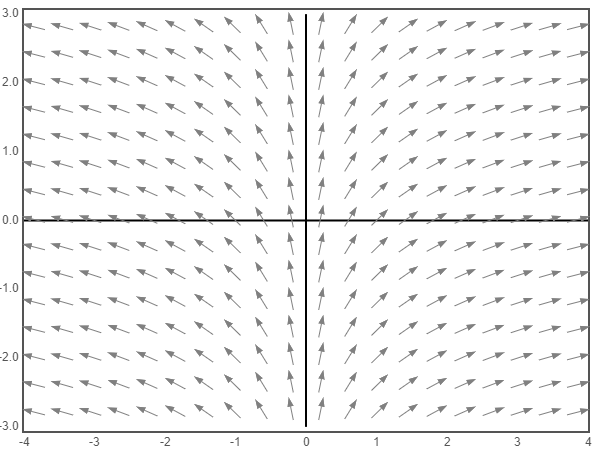
\includegraphics[width=\linewidth]{images/5-VecField1.png}
\end{image}%
 Thus a Phase Portrait would look like: \begin{image}{0}{1}{0}%
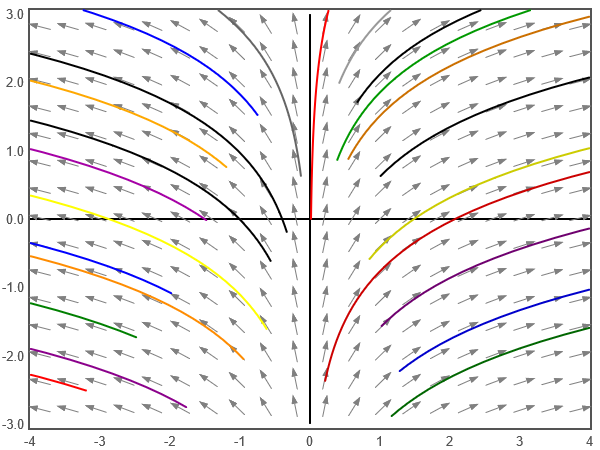
\includegraphics[width=\linewidth]{images/5-VecField1b.png}
\end{image}%
 Recall that a Phase portrait is simply several examples of solutions (which are Phase planes) to the system.%
\end{example}
\begin{example}{}{g:example:id518592}%
Consider the IVP%
\begin{align*}
x_{1}^{\prime} \amp =x_{1}\,\,\,\,\,\,,x_{1}(0)=-1\\
x_{2}^{\prime} \amp =1\,\,\,\,\,\,\,\,,x_{2}(0)=0
\end{align*}
Using the previous example, draw a rough sketch of the trajectory for the solution of this IVP on the Phase plane and predict the long term behavior of the solution. (In later sections, we will be able to draw better graphs without using the vector field, and we will be able to find the exact long term behavior without guessing)%
\par
\terminology{Solution}%
\par
By following the general direction of the vectors in the vector field above starting at the point \((-1,0)\) in the \(x_{1}-x_{2}\) plane we obtain: \begin{image}{0}{1}{0}%
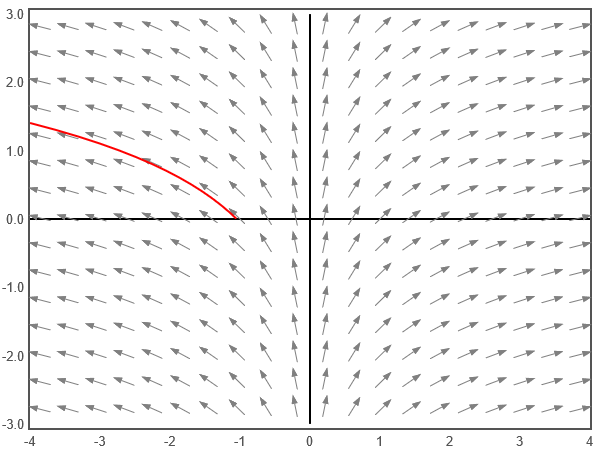
\includegraphics[width=\linewidth]{images/5-VecField1c.png}
\end{image}%
 Note that%
\begin{equation*}
\lim_{t\to\infty}x_{1}(t)=-\infty
\end{equation*}
%
\begin{equation*}
\lim_{t\to\infty}x_{2}(t)=+\infty
\end{equation*}
%
\end{example}
\begin{example}{}{g:example:id518654}%
Consider%
\begin{align*}
x_{1}^{\prime} \amp =x_{2}\\
x_{2}^{\prime} \amp =-2x_{1}
\end{align*}
Draw a rough sketch of the vector field. Use a computer software to draw a vector field. Then draw a rough Phase portrait based on this vector field. (In later sections, we will be able to draw exactly what the Phase portrait should look like without making guesses).%
\par
\terminology{Solution}%
\par
We again can use the following applet to draw the vector fields: \href{https://homepages.bluffton.edu/\~nesterd/apps/slopefields.html}{https:\slash{}\slash{}homepages.bluffton.edu\slash{}\textasciitilde{}nesterd\slash{}apps\slash{}slopefields.html} Using the vector Field \(\mathbf{F}(x_{1},x_{2})=\left(x_{2},-2x_{1}\right)\). We obtain: \begin{image}{0}{1}{0}%
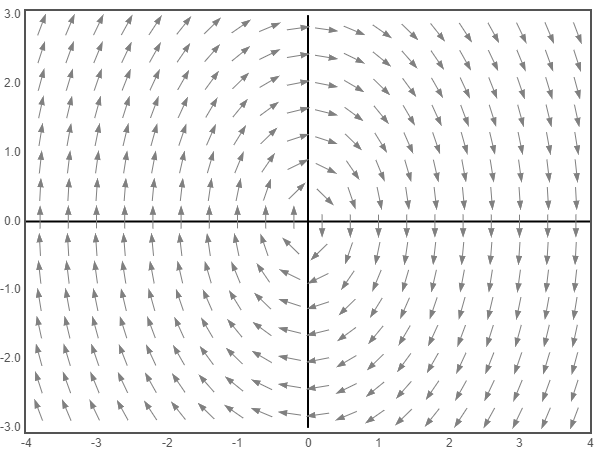
\includegraphics[width=\linewidth]{images/5-VecField2.png}
\end{image}%
 A Phase Portrait could be: \begin{image}{0}{1}{0}%
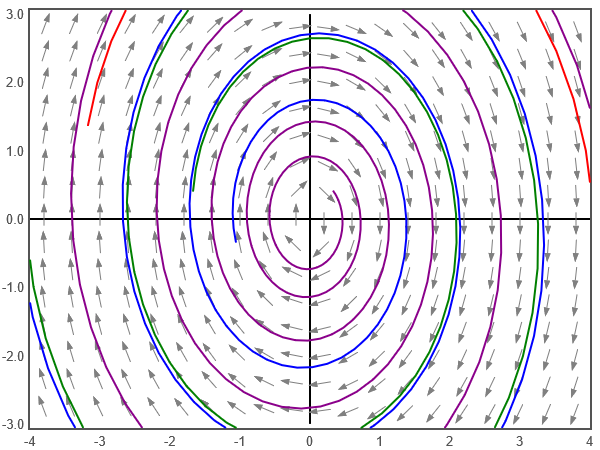
\includegraphics[width=\linewidth]{images/5-VecField2b.png}
\end{image}%
%
\end{example}
\end{subsectionptx}
\end{sectionptx}
%
%
\typeout{************************************************}
\typeout{Section 5.3 Systems of Linear Equations: Linear Independence, and the General Solution Theorem}
\typeout{************************************************}
%
\begin{sectionptx}{Systems of Linear Equations: Linear Independence, and the General Solution Theorem}{}{Systems of Linear Equations: Linear Independence, and the General Solution Theorem}{}{}{x:section:ch5-3}
%
%
\typeout{************************************************}
\typeout{Subsection 5.3.1 Crash course in linear algebra}
\typeout{************************************************}
%
\begin{subsectionptx}{Crash course in linear algebra}{}{Crash course in linear algebra}{}{}{g:subsection:id518660}
Suppose we want to find solutions to \(A\mathbf{x}=\mathbf{0}\) or%
\begin{equation*}
\left(\begin{array}{cc}
a \amp b\\
c \amp  d
\end{array}\right)\left(\begin{array}{c}
x_{1}\\
x_{2}
\end{array}\right)=\left(\begin{array}{c}
0\\
0
\end{array}\right)\mbox{ }\iff\begin{array}{c}
ax_{1}+bx_{2}=0\\
cx_{1}+dx_{2}=0
\end{array}\mbox{ }
\end{equation*}
take%
\begin{equation*}
\left(\begin{array}{cc}
1 \amp  2\\
-1 \amp 3
\end{array}\right)\left(\begin{array}{c}
x_{1}\\
x_{2}
\end{array}\right)=\left(\begin{array}{c}
0\\
0
\end{array}\right)\mbox{ }\iff\begin{array}{c}
x_{1}+2x_{2}=0\\
-x_{1}+3x_{2}=0
\end{array}
\end{equation*}
or even%
\begin{equation*}
\left(\begin{array}{ccc}
1 \amp  0 \amp  1\\
1 \amp  0 \amp  0\\
1 \amp  1 \amp  1
\end{array}\right)\left(\begin{array}{c}
x_{1}\\
x_{2}\\
x_{3}
\end{array}\right)=\left(\begin{array}{c}
x_{1}\\
x_{2}\\
x_{3}
\end{array}\right)\mbox{ }\iff\begin{array}{c}
x_{1}+x_{3}=0\\
x_{1}=0\\
x_{1}+x_{2}+x_{3}=0
\end{array}
\end{equation*}
In general, one can find solutions to%
\begin{equation*}
A\mathbf{x}=\mathbf{0}
\end{equation*}
by using algebra on the system of equations, or by row-reducing (Gaussian elimination) the matrix. Notice that \(\mathbf{x}=\left(x_{1},x_{2}\right)=\left(0,0\right)\) is always a solution to%
\begin{equation*}
\begin{array}{c}
ax_{1}+bx_{2}=0\\
cx_{1}+dx_{2}=0
\end{array}.
\end{equation*}
But when do we have non-trivial (non-zero) solutions? In fact, there is a way to knowing if there are any non-trivial solutions without actually soliving the equation \(A\mathbf{x}=0\).%
\par
Recall, that the \terminology{determinant} of a matrix \(A=\left(\begin{array}{cc}
a \amp b\\
c \amp d
\end{array}\right)\) is defined to be%
\begin{equation*}
\det A=ad-bc
\end{equation*}
The \terminology{determinant} of a matrix \(A=\left(\begin{array}{cc}
1 \amp 2\\
-1 \amp 3
\end{array}\right)\) is defined to be%
\begin{equation*}
\det A=3-\left(-2\right)=5
\end{equation*}
Similarly, one can define determinants in higher dimensional setting. For example,%
\begin{equation*}
\det\left(\begin{array}{ccc}
a_{1,1} \amp a_{1,2} \amp a_{1,3}\\
a_{2,1} \amp a_{2,2} \amp a_{2,3}\\
a_{3,1} \amp a_{3,2} \amp a_{3,3}
\end{array}\right)=a_{1,1}\det\left(\begin{array}{cc}
a_{2,2} \amp a_{2,3}\\
a_{3,2} \amp a_{3,3}
\end{array}\right)-a_{1,2}\det\left(\begin{array}{cc}
a_{2,1} \amp a_{2,3}\\
a_{3,1} \amp a_{3,3}
\end{array}\right)+a_{1,3}\det\left(\begin{array}{cc}
a_{2,1} \amp a_{2,2}\\
a_{3,1} \amp a_{3,2}
\end{array}\right).
\end{equation*}
We have the following theorem:%
\begin{theorem}{}{}{x:theorem:thmlinalg1}%
If \(A\) is a matrix and \(\det A\neq0\) then the only solutions to the system \(A\mathbf{x}=\mathbf{0}\) is the \(\mathbf{x}=\mathbf{0}\), the origin.%
\par
If \(\det A=0\) then there are infinitely many solutions \(\mathbf{x}\). (In 2 dimensions , this means there is a whole line of solutions)%
\end{theorem}
Note that \(\det\left(\begin{array}{cc}
2 \amp 6\\
1 \amp 3
\end{array}\right)=0\) and hence there are nontrivial solutions to the equation \(\left(\begin{array}{cc}
2 \amp 6\\
1 \amp 3
\end{array}\right)\mathbf{x}=0\). For example, it is easy to check that \(\left(-3,1\right)\) is a nontrivial solution since%
\begin{equation*}
\left(\begin{array}{cc}
2 \amp 6\\
1 \amp 3
\end{array}\right)\left(\begin{array}{c}
-3\\
1
\end{array}\right)=\left(\begin{array}{c}
-6+6\\
-3+3
\end{array}\right)=\left(\begin{array}{c}
0\\
0
\end{array}\right)=\mathbf{0}
\end{equation*}
If \(\det A=0\) are then \(A\) is \terminology{singular}, or \terminology{degenerate}. If \(\det A\neq0\), then \(A\) is said to be \terminology{nonsingular}, or \terminology{nondegenerate}, or \terminology{invertible}. When \(A\) is invertible then the inverse matrix \(A^{-1}\) exists and we can solve%
\begin{equation*}
A\mathbf{x}=\mathbf{b}\,\,\,\,(\star)
\end{equation*}
by%
\begin{equation*}
\mathbf{x}=A^{-1}\mathbf{b}
\end{equation*}
and this is the \terminology{unique} solution to \((\star)\).%
\end{subsectionptx}
%
%
\typeout{************************************************}
\typeout{Subsection 5.3.2 Linear Independence}
\typeout{************************************************}
%
\begin{subsectionptx}{Linear Independence}{}{Linear Independence}{}{}{g:subsection:id518847}
Another important concept in linear algebra is when two vectors are \terminology{independent} or \terminology{dependent}. If \(\mathbf{x}=\left(\begin{array}{c}
x_{1}\\
x_{2}
\end{array}\right)\) and \(\mathbf{y}=\left(\begin{array}{c}
y_{1}\\
y_{2}
\end{array}\right)\) are vectors, then \(c_{1}\mathbf{x}+c_{2}\mathbf{y}\) is said to be a \terminology{linear combination} of the two vectors. For example, the vector \(\left(\begin{array}{c}
-3\\
8
\end{array}\right)\) is a linear combination of \(\left(\begin{array}{c}
1\\
2
\end{array}\right)\) and \(\left(\begin{array}{c}
-2\\
3
\end{array}\right)\). Why? Because if we let \(c_{1}=1\) and \(c_{2}=2\) note that%
\begin{equation*}
1\left(\begin{array}{c}
1\\
2
\end{array}\right)+2\left(\begin{array}{c}
-2\\
3
\end{array}\right)=\left(\begin{array}{c}
1\\
2
\end{array}\right)+\left(\begin{array}{c}
-4\\
6
\end{array}\right)=\left(\begin{array}{c}
-3\\
8
\end{array}\right).
\end{equation*}
%
\begin{assemblage}{}{x:assemblage:lininde}%
The vectors \(\mathbf{x}=\left(\begin{array}{c}
x_{1}\\
x_{2}
\end{array}\right)\) and \(\mathbf{y}=\left(\begin{array}{c}
y_{1}\\
y_{2}
\end{array}\right)\) are said to be \terminology{linearly independent} if the only solutions to \(c_{1}\mathbf{x}+c_{2}\mathbf{y}=\mathbf{0}\) are the trivial solutions \(c_{1}=c_{2}=0\).%
\end{assemblage}
A visual (and very useful) way to understand this, is that two vectors are \terminology{linearly independent} if they do not lie in the same line through the origin. One can think of two vectors being linearly \terminology{dependent} if they do lie in the same line. This idea can be generalized in higher dimension. For example, The 3-dimensional vectors \(\mathbf{x},\mathbf{y},\textbf{z}\) are \terminology{linearly indepedent} if the only solution to \(c_{1}\mathbf{x}+c_{2}\mathbf{y}+c_{3}\mathbf{z}=\mathbf{0}\) are the trivial solutions \(c_{1}=c_{2}=c_{3}=0\).%
\begin{example}{}{g:example:id518954}%
Are \(\mathbf{x}=\left(\begin{array}{c}
1\\
2
\end{array}\right)\) and \(\mathbf{y}=\left(\begin{array}{c}
3\\
4
\end{array}\right)\) linearly independent?%
\par
\terminology{Method1:} Note%
\begin{align*}
c_{1}\left(\begin{array}{c}
1\\
2
\end{array}\right)+c_{2}\left(\begin{array}{c}
3\\
4
\end{array}\right)=0 \amp \iff c_{1}\left(\begin{array}{c}
1\\
2
\end{array}\right)+c_{2}\left(\begin{array}{c}
3\\
4
\end{array}\right)=0\\
\amp \iff  \left(\begin{array}{c}
c_{1}+3c_{2}\\
2c_{1}+4c_{2}
\end{array}\right)=0\\
\amp \iff \left(\begin{array}{cc}
1 \amp 3\\
2 \amp 4
\end{array}\right)\left(\begin{array}{c}
c_{1}\\
c_{2}
\end{array}\right)=0\\
\amp \iff  \det\left(\begin{array}{cc}
1 \amp 3\\
2 \amp 4
\end{array}\right)=4-6\neq 0
\end{align*}
and from \hyperref[x:theorem:thmlinalg1]{Theorem~{\xreffont\ref{x:theorem:thmlinalg1}}} this tells us that they only solution is the trivial solution \(c_{1}=c_{2}=0\) . Hence yes! \terminology{linearly independent}!%
\par
Note that to check linear independence, all we needed to check was if%
\begin{equation*}
\det\left(\begin{array}{cc}
\mathbf{x} \amp \mathbf{y}\end{array}\right)\neq0.
\end{equation*}
%
\par
\terminology{Method2:} Draw this on the \(x-y\) plane and note they're NOT on the same line through the origin. Hence they are linearly independent.%
\end{example}
\begin{example}{}{g:example:id518988}%
Are \(\mathbf{x}=\left(\begin{array}{c}
3\\
-5
\end{array}\right)\) and \(\mathbf{y}=\left(\begin{array}{c}
-6\\
10
\end{array}\right)\) linearly independent?%
\par
\terminology{Method1:} Note that%
\begin{align*}
c_{1}\left(\begin{array}{c}
3\\
-5
\end{array}\right)+c_{2}\left(\begin{array}{c}
-6\\
10
\end{array}\right)=0  \amp \iff  \left(\begin{array}{cc}
3 \amp -6\\
-5 \amp 10
\end{array}\right)\left(\begin{array}{c}
c_{1}\\
c_{2}
\end{array}\right)=0\\
\amp \iff  \det\left(\begin{array}{cc}
3 \amp -6\\
-5 \amp 10
\end{array}\right)=30-30=0 
\end{align*}
and from \hyperref[x:theorem:thmlinalg1]{Theorem~{\xreffont\ref{x:theorem:thmlinalg1}}} this tells us there are infinitely many solutions. Hence these vectors are \terminology{linearly dependent!}.%
\par
Again, note that alternatively, to check \(\mathbf{x}\) and \(\mathbf{y}\) are linearly dependent, then it suffices to check that%
\begin{equation*}
\det\left(\begin{array}{cc}
\mathbf{x} \amp \mathbf{y}\end{array}\right)=\det\left(\begin{array}{cc}
3 \amp -6\\
-5 \amp 10
\end{array}\right)=0.
\end{equation*}
%
\par
\terminology{Method2:} Draw this on the \(x-y\) plane and note they ARE on the same line through the origin. Hence, they are linearly dependent.%
\end{example}
\end{subsectionptx}
%
%
\typeout{************************************************}
\typeout{Subsection 5.3.3 Equilibrium Solutions}
\typeout{************************************************}
%
\begin{subsectionptx}{Equilibrium Solutions}{}{Equilibrium Solutions}{}{}{g:subsection:id519034}
Let's get back to differential equations. Consider the system:%
\begin{equation*}
\frac{d\mathbf{x}}{dt}=A\mathbf{x}
\end{equation*}
which we sometimes also write as%
\begin{equation*}
\mathbf{x}^{\prime}=A\mathbf{x}
\end{equation*}
where \(A=\left(\begin{array}{cc}
a \amp b\\
c \amp d
\end{array}\right)\) and \(\mathbf{x}=\left(\begin{array}{c}
x_{1}\\
x_{2}
\end{array}\right)\). Recall that an \terminology{Equilibrium Solution}, is a constant function \(\mathbf{x}(t)=\left(x_{0},y_{0}\right)\) such that \(\frac{d\mathbf{x}}{dt}=A\mathbf{x}=\mathbf{0}\). That is if%
\begin{equation*}
\left(\begin{array}{cc}
a \amp b\\
c \amp d
\end{array}\right)\left(\begin{array}{c}
x_{1}\\
X_{2}
\end{array}\right)=0\iff\left(\begin{array}{c}
ax_{1}+bx_{2}\\
cx_{1}+dx_{2}
\end{array}\right)=\left(\begin{array}{c}
0\\
0
\end{array}\right).
\end{equation*}
So this just boiled downed to a linear algebra problem and we can restate \hyperref[x:theorem:thmlinalg1]{Theorem~{\xreffont\ref{x:theorem:thmlinalg1}}} in differential equations language.%
\begin{theorem}{}{}{x:theorem:diffeq-system-eqsol}%
If \(A\) is the coefficient matrix then%
\par
(1) If \(\det A\neq0\), then the only equilibrium solution to \(\frac{d\mathbf{x}}{dt}=A\mathbf{x}\) is \(\mathbf{x}=(x_{1}(t),x_{2}(t))=\left(0,0\right)\).%
\par
(2) If \(\det A=0\) , then we have an infinite number of equilibrium solution. (In fact, an entire line of equilibrum solutions in 2 dimensions)%
\end{theorem}
\begin{example}{}{g:example:id519088}%
Consider, \(\frac{d\mathbf{x}}{dt}=A\mathbf{x}\) for \(A=\left(\begin{array}{cc}
1 \amp 2\\
3 \amp 4
\end{array}\right)\) , then \(\det A=4-6=-2\) which means \(\mathbf{x}(t)=\left(0,0\right)\) is the only Equilibrium Solution.%
\end{example}
\begin{example}{}{g:example:id519133}%
Consider \(\frac{d\mathbf{x}}{dt}=A\mathbf{x}\) for \(A=\left(\begin{array}{cc}
2 \amp -4\\
-1 \amp 2
\end{array}\right)\) . Then since \(\det A=0\) then there are an infinite number of equilibrium solutions.%
\end{example}
\end{subsectionptx}
%
%
\typeout{************************************************}
\typeout{Subsection 5.3.4 Linearity principle and the General Solution Theorem}
\typeout{************************************************}
%
\begin{subsectionptx}{Linearity principle and the General Solution Theorem}{}{Linearity principle and the General Solution Theorem}{}{}{g:subsection:id519128}
We start with the Linearity principle.%
\begin{theorem}{}{}{x:theorem:diffeq-system-linprin}%
Suppose \(\mathbf{x}^{\prime}=A\mathbf{x}\) is a linear system of differential equations.%
\par
(1) If \(\mathbf{x}(t)\) is a solution of this system and \(c\) is any constnat, then \(c\mathbf{x}(t)\) is also a solution.%
\par
(2) If \(\mathbf{x}^{(1)}(t)\) and \(\mathbf{x}^{(2)}(t)\) are two solutions of this system, then \(c_{1}\mathbf{x}^{(1}(t)+c_{2}\mathbf{x}^{(2)}(t)\) is also a solution.%
\end{theorem}
The point is that we can create new solutions from ones we already know are solutions via linear combinations! In fact, as long as I have one solution then I have infinitely many. We'll see that if as long as we have two solutions that are \terminology{linearly independent}, then we have all possible solutions. (i.e. the general solution)%
\begin{theorem}{}{}{x:theorem:diffeq-system-Wronskian}%
Two solutions \(\mathbf{x}^{(1)}(t),\mathbf{x}^{(1)}(t)\) are \terminology{linearly independent} if and only if the \terminology{Wronskian}%
\begin{equation*}
W\left[\mathbf{x}^{(1)},\mathbf{x}^{(2)}\right]:=\det\left(\mathbf{x}^{(1)}(t),\mathbf{x}^{(2)}(t)\right)\neq0,
\end{equation*}
for some \(t=t_{0}\).%
\end{theorem}
\begin{proof}{}{g:proof:id519231}
The idea of the proof is to check \(\mathbf{x}^{(1)}(t),\mathbf{x}^{(1)}(t)\) are linearly independent, then we must check that the only solutions two%
\begin{equation*}
c_{1}\mathbf{x}^{(1)}(t)+\mathbf{x}^{(1)}(t)=\mathbf{0}
\end{equation*}
is the trivial solution \(c_{1}=0\) and \(c_{2}=0\) for all \(t\). But, by \hyperref[x:theorem:thmlinalg1]{Theorem~{\xreffont\ref{x:theorem:thmlinalg1}}}, this happens if and only if%
\begin{equation*}
\det\left(\mathbf{x}^{(1)}(t),\mathbf{x}^{(2)}(t)\right)\neq0.
\end{equation*}
We leave it as an excercise to show that if \(\det\left(\mathbf{x}^{(1)}(t),\mathbf{x}^{(2)}(t)\right)\neq0\) for some \(t_{0}\), then it must be true for all \(t\).%
\end{proof}
We can finally state the General Solution Theorem.%
\begin{theorem}{The General Solution theorem.}{}{x:theorem:diffeq-system-genthm}%
Suppose \(\mathbf{x}^{(1)}(t)\) and \(\mathbf{x}^{(2)}(t)\) are solutions of the system \(\mathbf{x}^{\prime}=A\mathbf{x}\). If \(\mathbf{x}^{(1)}(0)\) and \(\mathbf{x}^{(1)}(0)\) are linearly independent, then for any initial condition \(\mathbf{x}(0)=\left(x_{0},y_{0}\right)\), we can find constants \(c_{1}\) and \(c_{2}\) such that \(\mathbf{x}(t)=c_{1}\mathbf{x}^{(1)}(t)+c_{2}\mathbf{x}^{(1)}(t)\) is the solution to the IVP%
\begin{equation*}
\mathbf{x}^{\prime}=A\mathbf{x},\,\,\,\,\mathbf{x}(0)=\left(\begin{array}{c}
x_{0}\\
y_{0}
\end{array}\right).
\end{equation*}
%
\par
Moreover, this means that if the Wronskian, \(W\left[\mathbf{x}^{(1)},\mathbf{x}^{(2)}\right]=\det\left(\mathbf{x}^{(1)}(t),\mathbf{x}^{(2)}(t)\right)\neq0\), then the general solution to%
\begin{equation*}
\mathbf{x}^{\prime}=A\mathbf{x}
\end{equation*}
is given by%
\begin{equation*}
\mathbf{x}(t)=c_{1}\mathbf{x}^{(1)}(t)+c_{2}\mathbf{x}^{(1)}(t)
\end{equation*}
%
\end{theorem}
\terminology{Overview:}%
\par
Thus \hyperref[x:theorem:diffeq-system-genthm]{Theorem~{\xreffont\ref{x:theorem:diffeq-system-genthm}}} says that as long as we can find two \terminology{linearly independent} solutions \(\mathbf{x}^{(1)}(t)\) and \(\mathbf{x}^{(2)}(t)\) (that is \(W\left[\mathbf{x}^{(1)},\mathbf{x}^{(2)}\right]\neq 0\) for some \(t\)) then every solution (i.e. the \terminology{General Solution} ) is of the form%
\begin{equation*}
\mathbf{x}(t)=c_{1}\mathbf{x}^{(1)}(t)+c_{2}\mathbf{x}^{(1)}(t).
\end{equation*}
%
\begin{example}{}{g:example:id519375}%
Suppose you already know that \(\mathbf{x}^{(1)}(t)=\left(\begin{array}{c}
1\\
-2
\end{array}\right)e^{-4t}\) and \(\mathbf{x}^{(2)}(t)=\left(\begin{array}{c}
3\\
2
\end{array}\right)e^{4t}\) are solutions to%
\begin{equation*}
\mathbf{x}^{\prime}=\left(\begin{array}{cc}
2 \amp 3\\
4 \amp -2
\end{array}\right)\mathbf{x}.
\end{equation*}
(In fact, part of this was checked in the previous section) Can you find the General solution to this system?%
\par
\terminology{Solution:}%
\par
We simply need to check if these solutions are linearly independent, that is we need to check that \(W\left[\mathbf{x}^{(1)},\mathbf{x}^{(2)}\right]=\det\left(\mathbf{x}^{(1)}(t),\mathbf{x}^{(2)}(t)\right)\neq0\) for some \(t\). Since%
\begin{align*}
W\left[\mathbf{x}^{(1)},\mathbf{x}^{(2)}\right] \amp =\left|\begin{array}{cc}
e^{-4t} \amp 3e^{4t}\\
-2e^{4t} \amp 2e^{4t}
\end{array}\right|\\
\amp =2-(-6)\\
\amp =8\\
\amp \neq 0 
\end{align*}
then these solutions are linearly independent. Hence by the General Solution Theorem \hyperref[x:theorem:diffeq-system-genthm]{Theorem~{\xreffont\ref{x:theorem:diffeq-system-genthm}}} we have that the General Solution is given by%
\begin{equation*}
\mathbf{x}(t)=c_{1}\left(\begin{array}{c}
1\\
-2
\end{array}\right)e^{-4t}+c_{2}\left(\begin{array}{c}
3\\
2
\end{array}\right)e^{4t}.
\end{equation*}
%
\end{example}
\end{subsectionptx}
\end{sectionptx}
%
%
\typeout{************************************************}
\typeout{Section 5.4 Basic Theory of Systems of 1st Order Linear EQs - Straight Line Solutions}
\typeout{************************************************}
%
\begin{sectionptx}{Basic Theory of Systems of 1st Order Linear EQs - Straight Line Solutions}{}{Basic Theory of Systems of 1st Order Linear EQs - Straight Line Solutions}{}{}{x:section:ch5-4}
%
%
\typeout{************************************************}
\typeout{Subsection 5.4.1 Eigenvalues and Eigenvectors}
\typeout{************************************************}
%
\begin{subsectionptx}{Eigenvalues and Eigenvectors}{}{Eigenvalues and Eigenvectors}{}{}{g:subsection:id519388}
Geometrically, an \terminology{eigenvector} is a vector where the vector field points in the same or opposite direction as the vector itself. For example, consider the following vector field:%
\begin{image}{0}{1}{0}%
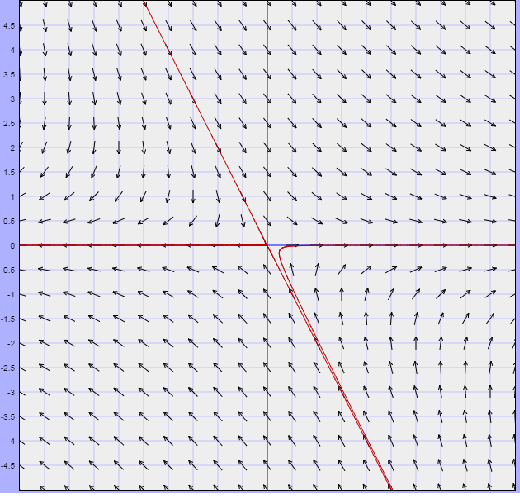
\includegraphics[width=\linewidth]{images/3.2 - system1.png}
\end{image}%
Then note that, the vectors in the directions of the straight-line are called \terminology{eigenvectors}.%
\begin{assemblage}{Eigenvalue\slash{}Eigenvectors.}{g:assemblage:id519417}%
Given a matrix \(A\), a number \(\lambda\) is called an \terminology{eigenvalue} of \(A\) if there is a nonzero vector \(\mathbf{v}\) such that%
\begin{equation*}
A\mathbf{v}=\lambda\mathbf{v}.
\end{equation*}
The corresponding vector \(\mathbf{v}\) is called an \terminology{eigenvector of the eigenvalue}  \(\lambda\).%
\end{assemblage}
Our goal is to demonstrate how to find eigenvalues and their corresponding eigenvectors of a given matrix%
\begin{equation*}
A=\left(\begin{array}{cc}
a \amp b\\
c \amp d
\end{array}\right).
\end{equation*}
First we find the eigenvalues, then we use the eigenvalue to find the corresponding eigenvectors. Let \(I=\left(\begin{array}{cc}
1 \amp 0\\
0 \amp 1
\end{array}\right)\) be the identity matrix then \(\lambda I=\left(\begin{array}{cc}
\lambda \amp 0\\
0 \amp \lambda
\end{array}\right)\). Note that by the definition of an eigenvalue, we must have that for some nonzero \(\mathbf{v}\), we have%
\begin{align*}
A\mathbf{v}=\lambda\mathbf{v} \amp \iff  A\mathbf{v}=\lambda\mathbf{v}\\
\amp \iff  A\mathbf{v}-\lambda\mathbf{v}=\mathbf{0} \\
\amp \iff  A\mathbf{v}-\lambda I\mathbf{v}=\mathbf{0}\\
\amp \iff  \left(A-\lambda I\right)\mathbf{v}=\mathbf{0}.
\end{align*}
Now \(A-\lambda I\) is actually another matrix. What matrix? Let's see,%
\begin{align*}
A-\lambda I \amp =  \left(\begin{array}{cc}
a \amp b\\
c \amp d
\end{array}\right)-\left(\begin{array}{cc}
\lambda \amp 0\\
0 \amp \lambda
\end{array}\right)\\
\amp =  \left(\begin{array}{cc}
a-\lambda \amp b\\
c \amp d-\lambda
\end{array}\right). 
\end{align*}
%
\par
So using \hyperref[x:theorem:thmlinalg1]{Theorem~{\xreffont\ref{x:theorem:thmlinalg1}}} from  \hyperref[x:section:ch5-3]{Section~{\xreffont\ref{x:section:ch5-3}}}, when do we know that the equation \(\left(A-\lambda I\right)\mathbf{v}=\mathbf{0}\) has nontrivial solution? Recall that \hyperref[x:theorem:thmlinalg1]{Theorem~{\xreffont\ref{x:theorem:thmlinalg1}}}  says that if%
\begin{equation*}
\det\left(A-\lambda I\right)=0,
\end{equation*}
then we have nontrivial solutions! Let's solve for \(\lambda\), because we know how to find determinants.%
\begin{align*}
\det\left(A-\lambda I\right)=0 \amp \iff  \det\left(\begin{array}{cc}
a-\lambda \amp b\\
c \amp d-\lambda
\end{array}\right)=0\\
\amp \iff  \left(a-\lambda\right)\left(d-\lambda\right)-bc=0.\\
\amp \iff  \left(\mbox{something}\right)\lambda^{2}+(\mbox{something})\lambda+(\mbox{something})=0 
\end{align*}
so solve for \(\lambda\) and that will be your eigenvalue! This polynomial is called the \terminology{characteristic polynomial}.%
\begin{example}{Finding eigenvalues and eigenvectors.}{x:example:example-ch5-4-1}%
Find the eigenvalues and a corresponding eigenvector of the matrix%
\begin{equation*}
A=\left(\begin{array}{cc}
2 \amp 3\\
0 \amp -4
\end{array}\right).
\end{equation*}
%
\par
\terminology{Step1:}Solve%
\begin{align*}
\det\left(A-\lambda I\right)=0 \amp \iff  \det\left(\begin{array}{cc}
2-\lambda \amp 3\\
0 \amp -4-\lambda
\end{array}\right)=0\\
\amp \iff  \left(2-\lambda\right)\left(-4-\lambda\right)-0\cdot3=0.\\
\amp \iff \left(2-\lambda\right)\left(-4-\lambda\right)=0\\
\amp \iff  \lambda=-4,2.
\end{align*}
%
\par
\terminology{Step2:} Find the eigenvectors: Let's start with \(\lambda_{1}=2\) then \(\mathbf{v}_{1}=\left(\begin{array}{c}
x_{1}\\
x_{2}
\end{array}\right)\) is an eigenvector if%
\begin{align*}
A\mathbf{v}=2\mathbf{v} \amp \iff  \left(\begin{array}{cc}
2 \amp 3\\
0 \amp -4
\end{array}\right)\left(\begin{array}{c}
x_{1}\\
x_{2}
\end{array}\right)=2\left(\begin{array}{c}
x_{1}\\
x_{2}
\end{array}\right)\\
\amp \iff  \left(\begin{array}{c}
2x_{1}+3x_{2}\\
-4x_{2}
\end{array}\right)=2\left(\begin{array}{c}
x_{1}\\
x_{2}
\end{array}\right)\\
\amp \iff  \begin{cases}
2x_{1}+3x_{2}=2x_{1}\\
-4x_{2}=2x_{2}
\end{cases}\\
\amp \iff  x_{2}=0\mbox{ and }x_{1}=\mbox{can be anything.} 
\end{align*}
so choose \(\mathbf{v}_{1}=\left(\begin{array}{c}
1\\
0
\end{array}\right)\) as an eigenvector.%
\terminology{Step3:} Find the corresponding eigenvectors: Now let \(\lambda_{2}=-4\) then \(\mathbf{v_{2}}=\left(\begin{array}{c}
x_{1}\\
x_{2}
\end{array}\right)\) is an eigenvector if%
\begin{align*}
A\mathbf{v}=-4\mathbf{v} \amp \iff \begin{cases}
2x_{1}+3x_{2}=-4x_{1}\\
-4x_{2}=-4x_{2}
\end{cases}\\
\amp \iff  \begin{cases}
6x_{1}+3x_{2}=0 \amp \implies x_{2}=-2x_{1}\\
-4x_{2}=-4x_{2}
\end{cases} 
\end{align*}
so plugging the equation \(x_{2}=-2x_{1}\) back into the vector we get%
\begin{align*}
\mathbf{v}_{2} \amp =\left(\begin{array}{c}
x_{1}\\
x_{2}
\end{array}\right) \\
\amp =\left(\begin{array}{c}
x_{1}\\
-2x_{1}
\end{array}\right)
\end{align*}
and since \(x_{1}\) can be anything, we can choose \(x_{1}=1\) and \(\mathbf{v}_{2}=\left(\begin{array}{c}
x_{1}\\
-2x_{1}
\end{array}\right)\) is an eigenvector of the matrix \(A\). Notice that any multiple of an eigenvector would also be an eigenvector themselves. So we could also have chosen%
\begin{equation*}
\mathbf{v}_{2}=-3\left(\begin{array}{c}
1\\
-2
\end{array}\right)=\left(\begin{array}{c}
-3\\
6
\end{array}\right).
\end{equation*}
Hence for any eigenvalue \(\lambda\) there are an infinite number of possible eigenvectors \(\mathbf{v}\) corresponding to \(\lambda\).%
\end{example}
\end{subsectionptx}
%
%
\typeout{************************************************}
\typeout{Subsection 5.4.2 Back to Systems of Differential Equations}
\typeout{************************************************}
%
\begin{subsectionptx}{Back to Systems of Differential Equations}{}{Back to Systems of Differential Equations}{}{}{g:subsection:id519681}
Why are eigenvalues and eigenvectors important and useful in differential equations? Consider the system%
\begin{equation*}
\mathbf{x}^{\prime}=\left(\begin{array}{cc}
2 \amp 3\\
0 \amp -4
\end{array}\right)\mathbf{x}
\end{equation*}
Its vector field looks like this:%
\begin{image}{0}{1}{0}%
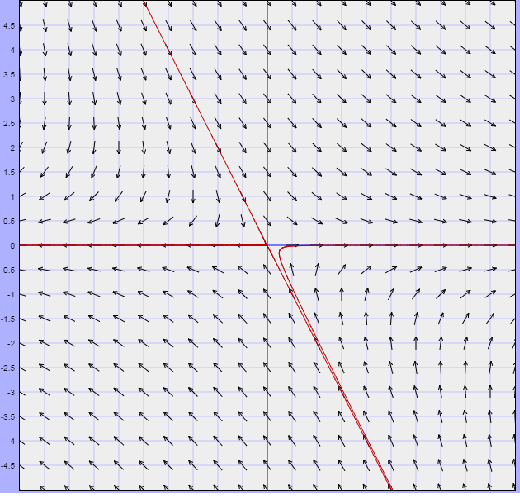
\includegraphics[width=\linewidth]{images/3.2 - system1.png}
\end{image}%
We want to search for \terminology{straight line solutions}.  Note that you see them on this vector field. We'd like to search for them because, for one, they probably have easy explicit formulas. And more importantly they are \terminology{linearly independent} (why? Because they are not in the same line), which will help build the general solution.%
\par
So how do we find them? From the geometry of the phase plane. If \(\mathbf{x}(t)\) is a straight-line solution, then notice that \(A\mathbf{x}=\lambda\mathbf{x}\) for some \(\lambda\). Because the vector \(A\mathbf{x}\) points in the same direction as the vector from \((0,0)\) to \(\mathbf{x}\). This means the solution \(\mathbf{x}(t)\) are formed from eigenvectors. So if we can find an eigenvector and its eigenvalue then we would have found a straight line solution.%
\begin{theorem}{}{}{x:theorem:thm-ch5-4-1}%
Suppose \(\lambda\) is an eigenvalue and \(\mathbf{v}=\left(\begin{array}{c}
x\\
y
\end{array}\right)\) is a corresponding eigevenvector. Then%
\begin{equation*}
\mathbf{x}(t)=e^{\lambda t}\left(\begin{array}{c}
x\\
y
\end{array}\right)=\left(\begin{array}{c}
e^{\lambda t}x\\
e^{\lambda t}y
\end{array}\right)
\end{equation*}
is a straight-line solution to the differential equation%
\begin{equation*}
\frac{d\mathbf{x}}{dt}=A\mathbf{x}.
\end{equation*}
%
\end{theorem}
\begin{proof}{}{g:proof:id520322}
We just have to check that the LHS and RHS are equal to each other in%
\begin{equation*}
\frac{d\mathbf{x}}{dt}=A\mathbf{x}.
\end{equation*}
%
\par
The Left-Hand-Side is%
\begin{equation*}
\frac{d\mathbf{x}}{dt}=\frac{d}{dt}\left(\begin{array}{c}
e^{\lambda t}x\\
e^{\lambda t}y
\end{array}\right)=\left(\begin{array}{c}
\lambda e^{\lambda t}x\\
\lambda e^{\lambda t}y
\end{array}\right)=\lambda\left(\begin{array}{c}
e^{\lambda t}x\\
e^{\lambda t}y
\end{array}\right)=\lambda\mathbf{x}
\end{equation*}
and the Right-Hand-Side is%
\begin{equation*}
A\mathbf{x}=Ae^{\lambda t}\mathbf{v}=e^{\lambda t}A\mathbf{v}=e^{\lambda t}\lambda\mathbf{v}=\lambda\left(e^{\lambda t}\mathbf{v}\right)=\lambda\mathbf{x}.
\end{equation*}
So yes they are equal, hence \(\mathbf{x}(t)=e^{\lambda t}\left(\begin{array}{c}
x\\
y
\end{array}\right)\) is a solution, and plotting this solution in the \(x_{1}-x_{2}\) plane, shows a moving particle moving in a straight-line.%
\end{proof}
We are now ready to solve  a vector differential equation with straight-line solutions.%
\begin{example}{}{g:example:id520380}%
Find the General solution to%
\begin{equation*}
\frac{d\mathbf{x}}{dt}=\left(\begin{array}{cc}
2 \amp 3\\
0 \amp -4
\end{array}\right)\mathbf{x}
\end{equation*}
%
\par
Recall that from \hyperref[x:example:example-ch5-4-1]{Example~{\xreffont\ref{x:example:example-ch5-4-1}}}, the matrix \(A=\left(\begin{array}{cc}
2 \amp 3\\
0 \amp -4
\end{array}\right)\) has the eigenvalue \(\lambda_{1}=2\) with an eigenvector \(\mathbf{v}_{1}=\left(\begin{array}{c}
1\\
0
\end{array}\right)\), and \(\lambda_{2}=-4\) with eigenvector \(\mathbf{v}_{2}=\left(\begin{array}{c}
1\\
-2
\end{array}\right)\). From \hyperref[x:theorem:thm-ch5-4-1]{Theorem~{\xreffont\ref{x:theorem:thm-ch5-4-1}}}, which we have just proved: Then we know two straight line solutions:%
\begin{equation*}
\mathbf{x}^{(1)}(t)=e^{2t}\left(\begin{array}{c}
1\\
0
\end{array}\right),\mbox{ and }\mathbf{x}^{(2)}(t)=e^{-4t}\left(\begin{array}{c}
1\\
-2
\end{array}\right).
\end{equation*}
If these are independent, then we can form the general solution using \hyperref[x:theorem:diffeq-system-genthm]{Theorem~{\xreffont\ref{x:theorem:diffeq-system-genthm}}}, the general solution theorem.  Take the Wronkian:%
\begin{equation*}
W\left[\mathbf{x}^{(1)},\mathbf{x}^{(2)}\right]=\left|\begin{array}{cc}
e^{2t} \amp e^{-4t}\\
0 \amp -2e^{-4t}
\end{array}\right|=-2e^{-2t}\neq0
\end{equation*}
hence \(\left\{ \mathbf{x}^{(1)},\mathbf{x}^{(2)}\right\} \) forms a \terminology{fundamental set of solutions}. Another way to show they are linearly indepenent is to remember that these vectors are in completely different lines and are not multiples of each other. Therefore they are independent! Thus the \terminology{general solution} is%
\begin{equation*}
\mathbf{x}(t)=c_{1}e^{2t}\left(\begin{array}{c}
1\\
0
\end{array}\right)+c_{2}e^{-4t}\left(\begin{array}{c}
1\\
-2
\end{array}\right).
\end{equation*}
%
\end{example}
We summarize this example into a Theorem. The key thing to remember here is that this theorem applies only to when you have \terminology{distinct} and \terminology{real} eigenvalues \(\lambda_{1},\lambda_{2}\).%
\begin{theorem}{Real and distinct eigenvalues.}{}{x:theorem:thm-ch5-4-2}%
Suppose \(A\) is a matrix with distinct, real eigenvalues \(\lambda_{1},\lambda_{2}\) with corresponding eigenvectors \(\mathbf{v}_{1},\mathbf{v}_{2}\), respectively. Then the \terminology{general solution} of the system%
\begin{equation*}
\mathbf{x}^{\prime}=A\mathbf{x}
\end{equation*}
is%
\begin{equation*}
\mathbf{x}(t)=c_{1}e^{\lambda_{1}t}\mathbf{v}_{1}+c_{2}e^{\lambda_{2}t}\mathbf{v}_{2}.
\end{equation*}
Moreover, the solutions \(\mathbf{x}^{(1)}(t)=e^{\lambda_{1}t}\mathbf{v}_{1},\mathbf{x}^{(2)}(t)=e^{\lambda_{2}t}\mathbf{v}_{2}\) are linearly independent.%
\end{theorem}
\end{subsectionptx}
\end{sectionptx}
%
%
\typeout{************************************************}
\typeout{Section 5.5 Phase Portraits for systems with real eigenvalues}
\typeout{************************************************}
%
\begin{sectionptx}{Phase Portraits for systems with real eigenvalues}{}{Phase Portraits for systems with real eigenvalues}{}{}{x:section:ch5-5}
\begin{introduction}{}%
Here are two facts we may have not noticed last time: If the eigenvalue \(\lambda\) is negative, then the straight line solution%
\begin{equation*}
\mathbf{x}(t)=e^{\lambda t}\mathbf{v}
\end{equation*}
tends to the origin \(\mathbf{0}\) as \(t\to\infty\). Take for example%
\begin{equation*}
\mathbf{x}(t)=e^{-t}\left(\begin{array}{c}
1\\
2
\end{array}\right)\text{,}
\end{equation*}
and note that%
\begin{equation*}
\lim_{t\to\infty}\mathbf{x}(t)=\left(\begin{array}{c}
0\\
0
\end{array}\right).
\end{equation*}
If the eigenvalue \(\lambda\) is positive, then straight line solution \(\mathbf{x}(t)=e^{\lambda t}\mathbf{v}\) tends away from the origin as \(t\to\infty\). In this section, we will consider the different types of behaviors one can obtain in the Phase plane for the trajectories of solutions. We study only the case when you have distinct real eigenvalues.%
\end{introduction}%
%
%
\typeout{************************************************}
\typeout{Subsection 5.5.1 Saddles}
\typeout{************************************************}
%
\begin{subsectionptx}{Saddles}{}{Saddles}{}{}{g:subsection:id520510}
We start with a definition.%
\begin{assemblage}{}{g:assemblage:id520528}%
A linear system for which we have one positive and one negative eigenvalue has an equilibrium point that is called a \terminology{saddle}.%
\end{assemblage}
\begin{example}{}{x:example:ex-ch5-5-1}%
Consider%
\begin{equation*}
\boldsymbol{x}^{\prime}=\left(\begin{array}{cc}
-3 \amp 0\\
0 \amp 2
\end{array}\right)\mathbf{x}
\end{equation*}
Draw a Phase portrait for this system.%
\par
\terminology{Solution:}%
\par
If we solve this system we get%
\begin{equation*}
\mathbf{x}(t)=c_{1}e^{-3t}\left(\begin{array}{c}
1\\
0
\end{array}\right)+c_{2}e^{2t}\left(\begin{array}{c}
0\\
1
\end{array}\right).
\end{equation*}
First draw straight line solutions in Phase Plane. The one associated to the negative eigenvalue will go towards the origin, while the one associated to the positive eigenvalue will go away from the origin. (as remarked in the introduction) Then draw other solutions in Phase Plane by following the vectors in the direction field. Recall by the Existence and Uniqueness Theorem that solutions can't cross. Hence other solutions can't cross the straight line soluions. Remember to include arrows in your trajectories to specify the direction that the solution is moving. And the Phase portrait looks like this: \begin{image}{0}{1}{0}%
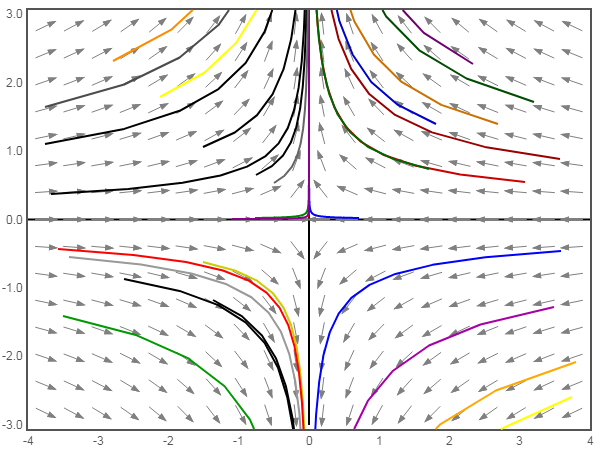
\includegraphics[width=\linewidth]{images/7.5b-1.png}
\end{image}%
%
\par
One thing to keep in mind is to note that the other solutions are moving in the general direction of the straight-line solutions without touching them.%
\end{example}
\begin{example}{}{x:example:ex-ch5-5-2}%
Consider the IVP%
\begin{equation*}
\mathbf{x}^{\prime}=\left(\begin{array}{cc}
-3 \amp 0\\
0 \amp 2
\end{array}\right)\mathbf{x},\,\,\,\,\mathbf{x}(0)=\left(\begin{array}{c}
-1\\
-1
\end{array}\right).
\end{equation*}
Draw the solution to this IVP in the Phase plane.%
\par
\terminology{Solution:}%
\par
Using the Phase portrait from \hyperref[x:example:ex-ch5-5-1]{Example~{\xreffont\ref{x:example:ex-ch5-5-1}}}, then the solution will have the following sketch: \begin{image}{0}{1}{0}%
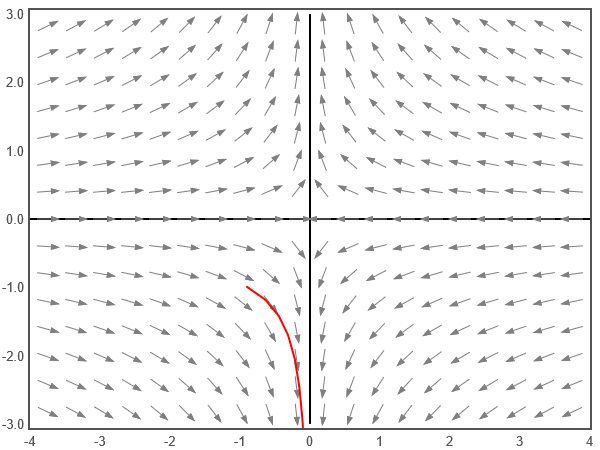
\includegraphics[width=\linewidth]{images/Ex5-5-1b.png}
\end{image}%
%
\end{example}
\begin{example}{}{x:example:ex-ch5-5-3}%
Consider%
\begin{equation*}
\mathbf{x}^{\prime}=\left(\begin{array}{cc}
8 \amp -11\\
6 \amp -9
\end{array}\right)\mathbf{x}
\end{equation*}
Draw a Phase portrait for this system.%
\par
\terminology{Solution:}%
\par
Solving for the eigenvalues\slash{}eigenvectors, we have%
\begin{equation*}
\begin{array}{ccc}
\lambda_{1}=-3, \amp  \amp \mathbf{v}_{1}=\left(\begin{array}{c}
1\\
1
\end{array}\right)\\
\lambda_{2}=2, \amp  \amp \mathbf{v}_{2}=\left(\begin{array}{c}
11\\
6
\end{array}\right)
\end{array}
\end{equation*}
hence we get%
\begin{equation*}
\mathbf{x}(t)=c_{1}e^{-3t}\left(\begin{array}{c}
1\\
1
\end{array}\right)+c_{2}e^{2t}\left(\begin{array}{c}
11\\
6
\end{array}\right).
\end{equation*}
%
\par
Using the same instructions as in \hyperref[x:example:ex-ch5-5-1]{Example~{\xreffont\ref{x:example:ex-ch5-5-1}}}, the Phase Portrait looks like this: \begin{image}{0}{1}{0}%
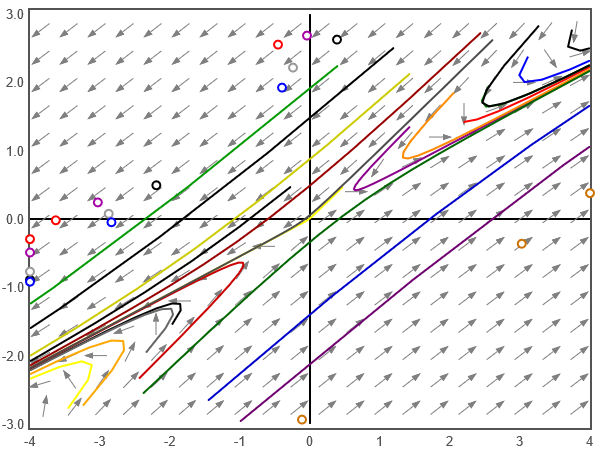
\includegraphics[width=\linewidth]{images/Ex5-5-3.png}
\end{image}%
%
\end{example}
\end{subsectionptx}
%
%
\typeout{************************************************}
\typeout{Subsection 5.5.2 Asymptotically stable node (sink)}
\typeout{************************************************}
%
\begin{subsectionptx}{Asymptotically stable node (sink)}{}{Asymptotically stable node (sink)}{}{}{g:subsection:id520599}
We start with a definition.%
\begin{assemblage}{}{g:assemblage:id520605}%
A linear system for which we have both negative, distinct eigenvalues has an equilibrium point that is called a \terminology{asymptotically stable node (sink)}.%
\end{assemblage}
\begin{example}{}{x:example:ex-ch5-5-4}%
Consider%
\begin{equation*}
\frac{d\mathbf{x}}{dt}=\left(\begin{array}{cc}
-1 \amp 0\\
0 \amp -4
\end{array}\right)\mathbf{x}.
\end{equation*}
Draw the Phase portrait.%
\par
\terminology{Solution:}%
\par
Solving for eigenvalues and eigenvectors we have%
\begin{equation*}
\begin{array}{ccc}
\lambda_{1}=-1, \amp  \amp \mathbf{v}_{1}=\left(\begin{array}{c}
1\\
0
\end{array}\right)\\
\lambda_{2}=-4, \amp  \amp \mathbf{v}_{2}=\left(\begin{array}{c}
0\\
1
\end{array}\right)
\end{array}
\end{equation*}
hence the general solution is given by%
\begin{equation*}
\mathbf{x}(t)=c_{1}e^{-t}\left(\begin{array}{c}
1\\
0
\end{array}\right)+c_{2}e^{-4t}\left(\begin{array}{c}
0\\
1
\end{array}\right).
\end{equation*}
%
\par
Now we draw the Phase portrait. First draw the straight line solutions in Phase Plane with arrows pointing inwards towards the origin. (This is because both eigenvalues are negative). Then draw the other solutions in the plane, which all converge to the origin. Note that the solutions come from the direction of the eigenvector that has the biggest magnitude. Note that \(\left|\lambda_{2}\right|=4>1=\left|\lambda_{1}\right|\), hence the straight line solution \(c_{2}e^{-4t}\left(\begin{array}{c}
0\\
1
\end{array}\right)\) has more strength. Hence all the other solution are coming from the direction \(e^{-4t}\left(\begin{array}{c}
0\\
1
\end{array}\right)\) pointing inwards.  And the Phase portrait looks like this: \begin{image}{0}{1}{0}%
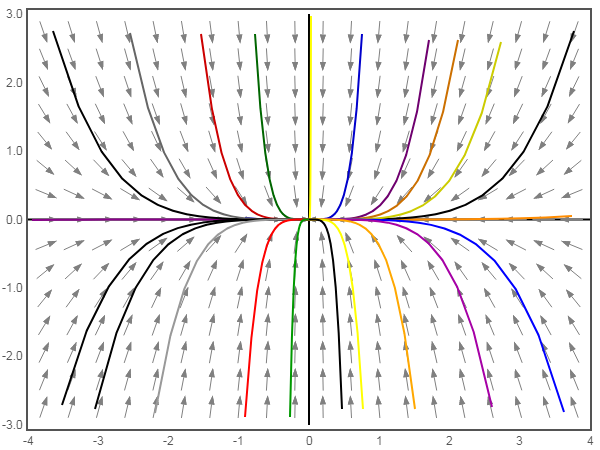
\includegraphics[width=\linewidth]{images/7.5b-2.png}
\end{image}%
 Note that soluions "sink" in.%
\end{example}
\begin{example}{}{x:example:ex-ch5-5-5}%
Consider%
\begin{equation*}
\frac{d\mathbf{x}}{dt}=\left(\begin{array}{cc}
-2 \amp -2\\
-1 \amp -3
\end{array}\right)\mathbf{x},
\end{equation*}
and suppose you know the eigenvalues\slash{}eigenvectors are given by%
\begin{equation*}
\begin{array}{ccc}
\lambda_{1}=-4, \amp  \amp \mathbf{v}_{1}=\left(\begin{array}{c}
1\\
1
\end{array}\right)\\
\lambda_{2}=-1, \amp  \amp \mathbf{v}_{2}=\left(\begin{array}{c}
-2\\
1
\end{array}\right)
\end{array}.
\end{equation*}
Draw the Phase portrait.%
\par
\terminology{Solution:}%
\par
First draw the straight line solutions in Phase Plane with arrows pointing inwards towards the origin. (This is because both eigenvalues are negative). Then draw the other solutions in the plane, which all converge to the origin. Note that the solutions come from the direction of the eigenvector that has the biggest magnitude. Note that \(\left|\lambda_{1}\right|=4>1=\left|\lambda_{2}\right|\), hence the straight line solution \(e^{-4t}\left(\begin{array}{c}
1\\
1
\end{array}\right)\) has more strength. Hence all the other solution are coming from the direction \(e^{-4t}\left(\begin{array}{c}
1\\
1
\end{array}\right)\) pointing inwards.  And the Phase portrait looks like this: \begin{image}{0}{1}{0}%
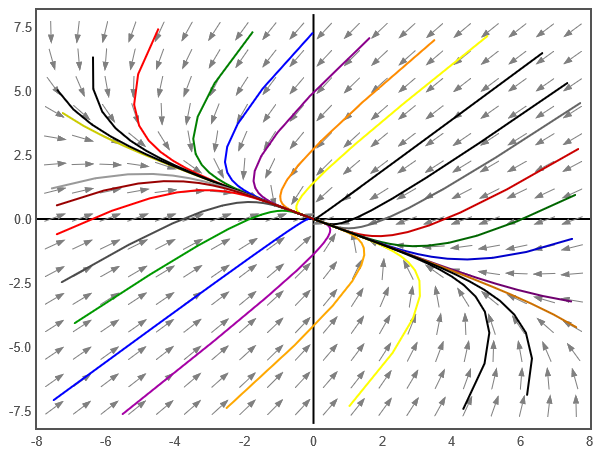
\includegraphics[width=\linewidth]{images/Ex5-5-5.png}
\end{image}%
 Note that soluions "sink" in.%
\end{example}
\end{subsectionptx}
%
%
\typeout{************************************************}
\typeout{Subsection 5.5.3 Asymptotically unstable node (source)}
\typeout{************************************************}
%
\begin{subsectionptx}{Asymptotically unstable node (source)}{}{Asymptotically unstable node (source)}{}{}{g:subsection:id520730}
We start with a definition.%
\begin{assemblage}{}{g:assemblage:id520727}%
A linear system for which we have both positive, distinct eigenvalues has an equilibrium point that is called a \terminology{asymptotically unstable node (source)}.%
\end{assemblage}
\begin{example}{}{x:example:ex-ch5-5-6}%
Consider%
\begin{equation*}
\frac{d\mathbf{x}}{dt}=\left(\begin{array}{cc}
2 \amp 2\\
1 \amp 3
\end{array}\right)\mathbf{x}.
\end{equation*}
Draw the Phase portrait.%
\par
\terminology{Solution:}%
\par
Solving for eigenvalues and eigenvectors we have%
\begin{equation*}
\begin{array}{ccc}
\lambda_{1}=4, \amp  \amp \mathbf{v}_{1}=\left(\begin{array}{c}
1\\
1
\end{array}\right)\\
\lambda_{2}=1, \amp  \amp \mathbf{v}_{2}=\left(\begin{array}{c}
-2\\
1
\end{array}\right)
\end{array}
\end{equation*}
hence the general solution is given by%
\begin{equation*}
\mathbf{x}(t)=c_{1}e^{4t}\left(\begin{array}{c}
1\\
1
\end{array}\right)+c_{2}e^{t}\left(\begin{array}{c}
-2\\
1
\end{array}\right).
\end{equation*}
%
\par
Now we draw the Phase portrait. First draw the straight line solutions in Phase Plane with arrows pointing outwards towards the origin. (This is because both eigenvalues are positive, hence the exponential explode away from the origin). Then draw the other solutions in the plane, which all converge explode away from the origin. Note that the solutions go towards the direction of the eigenvector that has the biggest magnitude. Note that \(\left|\lambda_{1}\right|=4>1=\left|\lambda_{2}\right|\), hence the straight line solution \(c_{2}e^{4t}\left(\begin{array}{c}
1\\
1
\end{array}\right)\) has more strength. Hence all the other solution are going towards the direction of \(e^{4t}\left(\begin{array}{c}
1\\
1
\end{array}\right)\) pointing outwards.  And the Phase portrait looks like this: \begin{image}{0}{1}{0}%
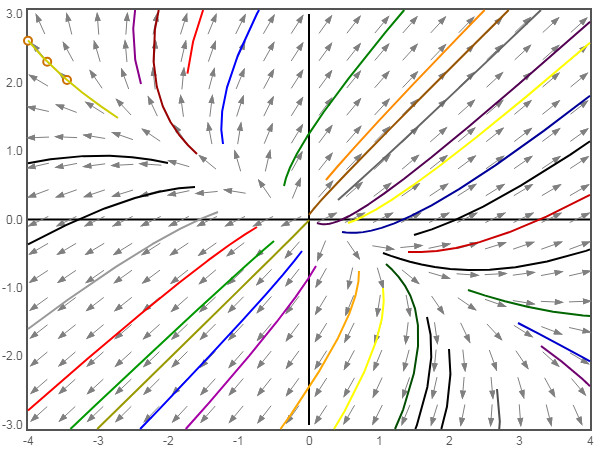
\includegraphics[width=\linewidth]{images/7.5b-3.png}
\end{image}%
 Note that solutions "source" out.%
\end{example}
\end{subsectionptx}
\end{sectionptx}
%
%
\typeout{************************************************}
\typeout{Section 5.6 Complex Eigenvalues}
\typeout{************************************************}
%
\begin{sectionptx}{Complex Eigenvalues}{}{Complex Eigenvalues}{}{}{x:section:ch5-6}
\begin{introduction}{}%
We have only worked when we have distinct real eigenvalues. But what if we get complex numbers as eigenvalues? When could this even happen? Consider the followig system:%
\begin{equation*}
\frac{d\mathbf{x}}{dt}=\left(\begin{array}{cc}
1 \amp -3\\
3 \amp 1
\end{array}\right)\mathbf{x}.
\end{equation*}
Before even trying to solve this system, let's plot its direction field:%
\par
\begin{image}{0}{1}{0}%
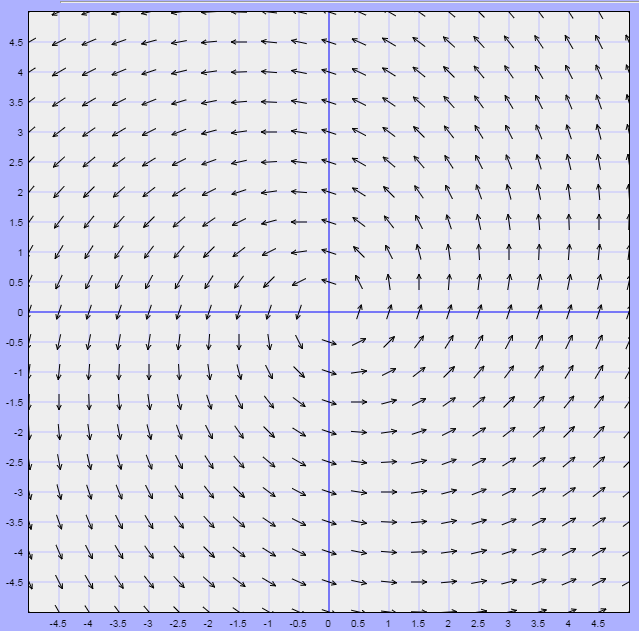
\includegraphics[width=\linewidth]{images/3.4-pic1.png}
\end{image}%
%
\par
The intuition from the previous two section no longer works. This is because ther are no straight line solutions. It looks like solutions will be spirals. So we shall proceed as have done before, by obtaining eigenvalues and eigenvector. But this time you will see that we will have complex eigenvalues and eigenvectors.%
\end{introduction}%
%
%
\typeout{************************************************}
\typeout{Subsection 5.6.1 Complex numbers:}
\typeout{************************************************}
%
\begin{subsectionptx}{Complex numbers:}{}{Complex numbers:}{}{}{g:subsection:id520781}
To make this section self-contained, we recall some basic facts about complex numbers. Complex numbers are of the form \(z = a+bi\) where \(a,b\in\mathbb{R}\) and \(i=\sqrt{-1}\). Thus \(i^{2}=-1\). Complex numbers have a \terminology{polar representation} \(z = r e^{i\theta}\), where \(r = \sqrt{a^2 + b^2}\) and \(\theta = \arctan\frac{y}{x}\). In the polar representation, we should think about \(r\) as a radius and \(e^{i\theta}\) as a point on the unit circle.%
\par
We should think about the exponential part as representing motion on a circle. The unit circle from trigonometry gives \((x,y) = (\cos \theta, \sin \theta)\) for an angle \(\theta\) on the unit circle. This connection is made explicit in what is known as \terminology{Euler's formula:}%
\begin{equation}
e^{i\theta}=\cos \theta+i\sin \theta.\label{x:men:Euler-chpt5}
\end{equation}
So%
\begin{equation*}
e^{a+ib}=e^{a}e^{ib}=e^{a}\left(\cos b+i\sin b\right)=e^{a}\cos b+ie^{a}\sin b.
\end{equation*}
%
\end{subsectionptx}
%
%
\typeout{************************************************}
\typeout{Subsection 5.6.2 Complex eigenvalues and eigenvectors}
\typeout{************************************************}
%
\begin{subsectionptx}{Complex eigenvalues and eigenvectors}{}{Complex eigenvalues and eigenvectors}{}{}{g:subsection:id520822}
The key ingredient when dealing with complex eigenvalues and eigenvectors is the following result. The following theorem should seem familiar. In fact, we saw a version of it in \hyperref[x:section:ch3-4]{Section~{\xreffont\ref{x:section:ch3-4}}} in \hyperref[x:theorem:thm-3-4-1]{Theorem~{\xreffont\ref{x:theorem:thm-3-4-1}}}.%
\begin{theorem}{}{}{x:theorem:thm-5-6-1}%
If \(\mathbf{x}_{c}(t)=\mathbf{x}_{re}(t)+i\mathbf{x}_{im}(t)\) is a solution to the linear system \(\frac{d\mathbf{x}}{dt}=A\mathbf{x}\). Then \(\mathbf{x}_{re}(t),\mathbf{x}_{im}(t)\) are themselves two linearly independent solutions to the system as well.%
\end{theorem}
Now we can consider the following example:%
\begin{example}{}{x:example:ex-ch5-6-1}%
Find the general solution to the following system:%
\begin{equation*}
\frac{d\mathbf{x}}{dt}=\left(\begin{array}{cc}
1 \amp -3\\
3 \amp 1
\end{array}\right)\mathbf{x}.
\end{equation*}
%
\par
\terminology{Solution:}%
\par
First we find the eigenvalues:%
\begin{align*}
\det\left(A-\lambda I\right)=0 \amp \iff\left|\begin{array}{cc}
1 \amp -\lambda-3\\
3 \amp 1-\lambda
\end{array}\right|=0\\
\amp \iff\left(1-\lambda\right)^{2}+9=0\\
\amp \iff\lambda=\frac{2\pm\sqrt{-36}}{2}=1\pm3i.
\end{align*}
\terminology{Pick one eigenvalue:} Say we pick \(\lambda_1 =-1+3i\). Now we find an eigenvector related to this eigenvalue. That is, we need to solve the eigenvalue-eigenvector equation:%
\begin{equation*}
A\mathbf{v}=\lambda\mathbf{v}
\end{equation*}
so that%
\begin{equation*}
\begin{cases}
x_{1}-3x_{2}=\left(1+3i\right)x_{1}\\
3x_{1}+x_{2}=\left(1+3i\right)x_{2}
\end{cases}
\end{equation*}
One of these equations will be redundant. So pick one equation to find an eigenvector:%
\begin{align*}
3x_{1}+x_{2}=\left(1+3i\right)x_{2} \amp \iff  3x_{1}=3ix_{2}\\
\amp \iff  x_{1}=ix_{2}\\
\amp \iff  \mbox{pick }x_{2}=1\mbox{ and get }x_{1}=i.
\end{align*}
So the eigenvector \(\mathbf{v}=\left(\begin{array}{c}
i\\
1
\end{array}\right)\) is associated with the eigenvalue \(\lambda=1+3i\).%
\par
\terminology{Find the corresponding complex solution:} (Let's call this solution \(\mathbf{x}_{c}(t)\))%
\begin{align*}
\mathbf{x}_{c}(t) \amp =  \mathbf{v}e^{\lambda t}\\
\amp =  \left(\begin{array}{c}
i\\
1
\end{array}\right)e^{\left(1+3i\right)t}\\
\amp =  \left(\begin{array}{c}
i\\
1
\end{array}\right)e^{t}e^{3ti}\\
\amp =  \left(\begin{array}{c}
i\\
1
\end{array}\right)e^{t}\left(\cos3t+i\sin3t\right)\mbox{ by Euler's Formula} \hyperref[x:men:Euler-chpt5]{\text{({\xreffont\ref{x:men:Euler-chpt5}})}}\\
\amp =  \left(\begin{array}{c}
ie^{t}\left(\cos3t+i\sin3t\right)\\
1e^{t}\left(\cos3t+i\sin3t\right)
\end{array}\right)\\
\amp =  \left(\begin{array}{c}
ie^{t}\cos3t-e^{t}\sin3t\\
e^{t}\cos3t+ie^{t}\sin3t
\end{array}\right)\\
\amp =  \left(\begin{array}{c}
-e^{t}\sin3t+ie^{t}\cos3t\\
e^{t}\cos3t+ie^{t}\sin3t
\end{array}\right)\mbox{put }i\mbox{'s together}\\
\amp =  \left(\begin{array}{c}
-e^{t}\sin3t\\
e^{t}\cos3t
\end{array}\right)+i\left(\begin{array}{c}
e^{t}\cos3t\\
e^{t}\sin3t
\end{array}\right)\\
\amp =  \mathbf{x}_{re}(t)+i\mathbf{x}_{im}(t).
\end{align*}
%
\par
By \hyperref[x:theorem:thm-5-6-1]{Theorem~{\xreffont\ref{x:theorem:thm-5-6-1}}}, we know that \(\mathbf{x}_{re}(t)\) and \(i\mathbf{x}_{im}(t)\) are two linearly independent solution. Thus by \hyperref[x:theorem:diffeq-system-genthm]{Theorem~{\xreffont\ref{x:theorem:diffeq-system-genthm}}}, the General Solution is given by%
\begin{equation*}
\mathbf{x}(t)=c_{1}\left(\begin{array}{c}
-e^{t}\sin3t\\
e^{t}\cos3t
\end{array}\right)+c_{2}\left(\begin{array}{c}
e^{t}\cos3t\\
e^{t}\sin3t
\end{array}\right)
\end{equation*}
%
\end{example}
\end{subsectionptx}
%
%
\typeout{************************************************}
\typeout{Subsection 5.6.3 Phase Portraits for complex eigenvalues}
\typeout{************************************************}
%
\begin{subsectionptx}{Phase Portraits for complex eigenvalues}{}{Phase Portraits for complex eigenvalues}{}{}{g:subsection:id520976}
We now discuss how to draw Phase portraits for complex eigenvalues case. We noted that in the beginning of the section that there were no straight-line solutions in this case. In fact, we usually see spirals.%
\begin{proposition}{}{}{x:proposition:prop-5-6-1}%
If a linear system \(\mathbf{x}^{\prime}=A\mathbf{x}\) has an eigenvalue \(\lambda=\alpha\pm\beta i\). Then the solution curves form spirals about the origin with natural period \(\frac{2\pi}{\beta}\), natural frequency \(\frac{\beta}{2\pi}\) and%
\par
(1) If \(\alpha  \lt 0 \), we call this an \terminology{asymptotically stable spiral point}. All solutions spiral in towards the origin \(\mathbf{0}\).%
\par
(2) If \(\alpha \gt 0\), we call this an \terminology{asymptotically unstable spiral point}. All solutions spiral away from the origin \(\mathbf{0}\).%
\par
(3) If \(\alpha = 0\), we call this a \terminology{center}. All solutions are elliptical shaped.%
\end{proposition}
\begin{example}{}{x:example:ex-ch5-6-2}%
Draw the Phase portrait for the system:%
\begin{equation*}
\frac{d\mathbf{x}}{dt}=\left(\begin{array}{cc}
1 \amp -3\\
3 \amp 1
\end{array}\right)\mathbf{x}.
\end{equation*}
which is solved in \hyperref[x:example:ex-ch5-6-1]{Example~{\xreffont\ref{x:example:ex-ch5-6-1}}}.%
\par
\terminology{Solution:}%
\par
Recall from \hyperref[x:example:ex-ch5-6-1]{Example~{\xreffont\ref{x:example:ex-ch5-6-1}}} that we have the complex roots \(\lambda=1\pm 3i \). Thus by \hyperref[x:proposition:prop-5-6-1]{Proposition~{\xreffont\ref{x:proposition:prop-5-6-1}}}, since \(\alpha=1 \gt 0 \), then the solution will have an \terminology{asymptotically unstable spiral} point. This means the solutions will be spirals coming from origin \(\mathbf{0}\). All that is left to do, is found out the direction of the spirals. To do this, it is enough to check the vector field \(\mathbf{F}(x,y)=A\mathbf{x}\) at two points. I usually check the vector field at points \(\(1,0)\) and \((0,1)\). We know that%
\begin{equation*}
\mathbf{F}\left(1,0\right)=\left(\begin{array}{cc}
1 \amp -3\\
3 \amp 1
\end{array}\right)\left(\begin{array}{c}
1\\
0
\end{array}\right)=\left(\begin{array}{c}
1\\
3
\end{array}\right)
\end{equation*}
while%
\begin{equation*}
\mathbf{F}\left(0,1\right)=\left(\begin{array}{cc}
1 \amp -3\\
3 \amp 1
\end{array}\right)\left(\begin{array}{c}
0\\
1
\end{array}\right)=\left(\begin{array}{c}
-3\\
1
\end{array}\right).
\end{equation*}
By drawing these two vectors in their respective positions we get: \begin{image}{0}{1}{0}%
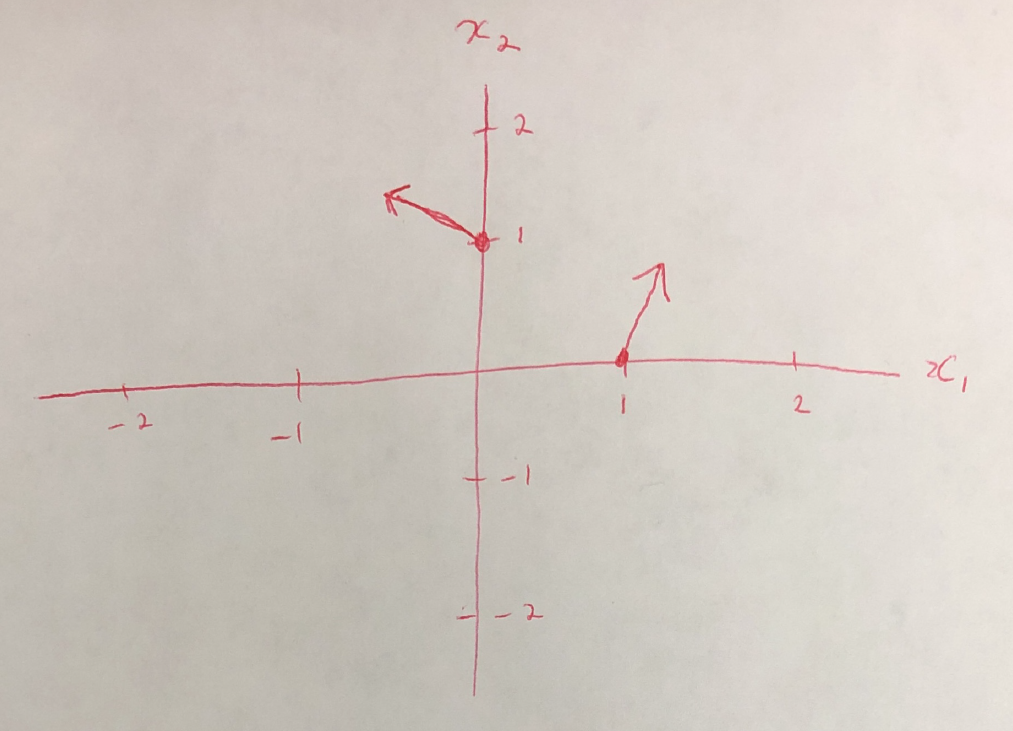
\includegraphics[width=\linewidth]{images/5.6-1c.png}
\end{image}%
 and from these two vector alone, we cansee that the direction of the spirals must be counter-clockwise. Hence, since these are unstable spirals we have the following Phase portrait: \begin{image}{0}{1}{0}%
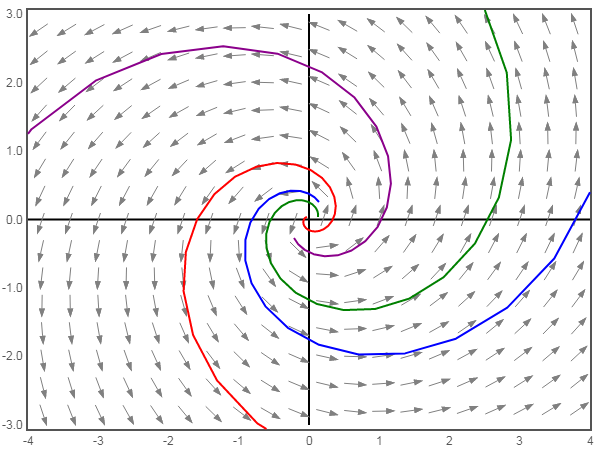
\includegraphics[width=\linewidth]{images/7.6-1.png}
\end{image}%
%
\end{example}
\end{subsectionptx}
\end{sectionptx}
%
%
\typeout{************************************************}
\typeout{Section 5.7 Repeated and zero eigenvalues}
\typeout{************************************************}
%
\begin{sectionptx}{Repeated and zero eigenvalues}{}{Repeated and zero eigenvalues}{}{}{x:section:ch5-7}
%
%
\typeout{************************************************}
\typeout{Subsection 5.7.1 Repeated real eigenvalues}
\typeout{************************************************}
%
\begin{subsectionptx}{Repeated real eigenvalues}{}{Repeated real eigenvalues}{}{}{g:subsection:id521102}
Suppose%
\begin{equation*}
\frac{d\mathbf{x}}{dt}=\left(\begin{array}{cc}
1 \amp -2\\
2 \amp 5
\end{array}\right)\mathbf{x}.
\end{equation*}
Let's first find the \terminology{eigenvalues}:%
\begin{align*}
\det\left(\begin{array}{cc}
1-\lambda  -2\\
2 \amp 5-\lambda
\end{array}\right)=0 
\amp \iff  \left(1-\lambda\right)\left(5-\lambda\right)+4=0\\
\amp \iff  \lambda^{2}-6\lambda+9=0\\
\amp \iff  \left(\lambda-3\right)^{2}=0,\\
\amp \iff \lambda=3,3.
\end{align*}
%
\par
Based on the intuition we've built from second order ODEs, in \hyperref[x:section:ch3-5]{Section~{\xreffont\ref{x:section:ch3-5}}}, it is reasonable to guess that the solution to this system will be of the form%
\begin{equation*}
\mathbf{x}(t)=e^{\lambda t}\mathbf{v}_{0}+te^{\lambda t}\mathbf{v}_{1}.
\end{equation*}
where \(\mathbf{x}(0)=\mathbf{v}_{0}\) is the initial condition. So what will \(\mathbf{v}_{1}\) be? Let's try figure it out. For this solution to work, we check that when plugging this \(\mathbf{x}\) into%
\begin{equation*}
\frac{d\mathbf{x}}{dt}=A\mathbf{x},
\end{equation*}
the Left-hand-side (LHS) equals to Right-hand-side(RHS) of the equation.%
\par
First let's compute the LHS, when plugging our guess into the equation,%
\begin{align*}
\frac{d\mathbf{x}}{dt} \amp =  \frac{d}{dt}\left(e^{\lambda t}\mathbf{v}_{0}+te^{\lambda t}\mathbf{v}_{1}\right)\\
\amp =  \lambda e^{\lambda t}\mathbf{v}_{0}+e^{\lambda t}\mathbf{v}_{1}+\lambda te^{\lambda t}\mathbf{v}_{1}\\
\amp =  \left(\lambda\mathbf{v}_{0}+\mathbf{v}_{1}\right)e^{\lambda t}+\left(\lambda\mathbf{v}_{1}\right)te^{\lambda t}
\end{align*}
%
\par
Now we plug our guess into the RHS,%
\begin{align*}
A\mathbf{x} \amp =  A\left(e^{\lambda t}\mathbf{v}_{0}+te^{\lambda t}\mathbf{v}_{1}\right)\\
\amp =  \left(A\mathbf{v}_{0}\right)e^{\lambda t}+\left(A\mathbf{v}_{1}\right)te^{\lambda t}
\end{align*}
So matching the coefficients of \(e^{\lambda t}\) and \(te^{\lambda t}\) in the LHS and RHS, we get that%
\begin{equation*}
\lambda\mathbf{v}_{1}=A\mathbf{v}_{1}\mbox{ and }\lambda\mathbf{v}_{0}+\mathbf{v}_{1}=A\mathbf{v}_{0}.
\end{equation*}
The first equation says that \(\mathbf{v}_{1}\) is either an eigenvector or the zero vector. But also, it must satisfy the second equation. Thus, by solving for \textdollar{}\textbackslash{}mathbf\textbraceleft{}v\textbraceright{}\textunderscore{}\textbraceleft{}1\textbraceright{}\textdollar{} in the second equation, we get that%
\begin{align*}
\lambda\mathbf{v}_{0}+\mathbf{v}_{1}=A\mathbf{v}_{0} \amp \iff  \mathbf{v}_{1}=A\mathbf{v}_{0}-\lambda\mathbf{v}_{0}\\
\amp \iff  \mathbf{v}_{1}=\left(A-\lambda I\right)\mathbf{v}_{0}.
\end{align*}
%
\par
Thus we summarize these computations in a theorem.%
\begin{theorem}{General Solution for repeated real eigenvalues.}{}{x:theorem:thm-5-7-1}%
Suppose \(\frac{d\mathbf{x}}{dt}=A\mathbf{x}\) is a system of which \(\lambda\) is a repeated real eigenvalue. Then the general solution is of the form:%
\begin{equation*}
\mathbf{x}(t)=e^{\lambda t}\mathbf{v}_{0}+te^{\lambda t}\mathbf{v}_{1}
\end{equation*}
where%
\begin{align*}
\mathbf{v}_{0} \amp =\mathbf{x}(0)\text{ (initial condition)}\\
\mathbf{v}_{1} \amp =\left(A-\lambda I\right)\mathbf{v}_{0}.
\end{align*}
Moreover, if \(\mathbf{v}_{1}\neq\mathbf{0}\) then it is an eigenvector with eigenvalue \(\lambda\), and if \(\mathbf{v}_{1}=0\) then \(\mathbf{v}_{0}\) is an eigenvector and \(\mathbf{x}(t)\) is a straight-line solution.%
\end{theorem}
\begin{assemblage}{Warning.}{g:assemblage:id521234}%
Never think that \(e^{\lambda t}\mathbf{v}_{0},te^{\lambda t}\mathbf{v}_{1}\) are generally solutions by themselves. This method is different than our usual method of finding two linearly independent solutions \(\mathbf{x}^{(1)}\) and \(\mathbf{x}^{(2)}\).%
\end{assemblage}
We can now do an example.%
\begin{example}{}{g:example:id521301}%
Find the solution to the following IVP:%
\begin{equation*}
\frac{d\mathbf{x}}{dt}=\left(\begin{array}{cc}
1 \amp -2\\
2 \amp 5
\end{array}\right)\mathbf{x},\,\,\,\,\,\mathbf{x}(0)=\left(\begin{array}{c}
2\\
1
\end{array}\right).
\end{equation*}
Then graph the phase portrait for the system and on a separate graph plot the particular solution to the IVP above.%
\par
\terminology{Solution:}%
\par
\terminology{Step 1:} Recall we found \(\lambda=3\) to be an eigenvalue in the discusion in the beginning of the section. We repeat the calculation here:%
\begin{align*}
\det\left(\begin{array}{cc}
1-\lambda  -2\\
2 \amp 5-\lambda
\end{array}\right)=0 
\amp \iff  \left(1-\lambda\right)\left(5-\lambda\right)+4=0\\
\amp \iff  \lambda^{2}-6\lambda+9=0\\
\amp \iff  \left(\lambda-3\right)^{2}=0,\\
\amp \iff \lambda=3,3.
\end{align*}
%
\par
\terminology{Step 2:} Suppose \(\mathbf{v}_{0}=\left(\begin{array}{c}
x_{0}\\
y_{0}
\end{array}\right)\) is the initial condition. Then we can compute \(\mathbf{v}_{1}\),%
\begin{align*}
\mathbf{v}_{1} \amp =  \left(A-\lambda I\right)\mathbf{v}_{0}\\
\amp =  \left(\begin{array}{cc}
-2 \amp -2\\
2 \amp 2
\end{array}\right)\left(\begin{array}{c}
x_{0}\\
y_{0}
\end{array}\right)\\
\amp =  \left(\begin{array}{c}
-2x_{0}-2y_{0}\\
2x_{0}+2y_{0}
\end{array}\right). 
\end{align*}
%
\par
\terminology{Step 3:} Write the \terminology{general solution}%
\begin{align*}
\mathbf{x}(t) \amp =  e^{3t}\mathbf{v}_{0}+te^{3t}\mathbf{v}_{1}\\
\amp =  e^{3t}\left(\begin{array}{c}
x_{0}\\
y_{0}
\end{array}\right)+te^{\lambda3t}\left(\begin{array}{c}
-2x_{0}-2y_{0}\\
2x_{0}+2y_{0}
\end{array}\right)
\end{align*}
and plugging the inital condition we have%
\begin{equation*}
\mathbf{x}(t)=e^{3t}\left(\begin{array}{c}
1\\
2
\end{array}\right)+te^{3t}\left(\begin{array}{c}
-6\\
6
\end{array}\right).
\end{equation*}
%
\par
\terminology{Step4:} We now make a phase portrait for the system. We plot the solutions by plotting the straight line solutions first (\(y=-x\)) which is associated to the eigenvector \(\mathbf{v}_1\) and then making the following graphs (an \terminology{almost spiral}, or more formally an \terminology{asymptotically unstable improper node}) with arrows pointing outwards (because \(\lambda=3>0\)). We call this an \terminology{almost spiral}, because solutions look like they are trying spiral around the equilibrium point \(\mathbf{0}\), but there's are straight-line solution blocking the other solutions from going around the origin. You should still check if the direction of the almost spirals are clockwise\slash{}counterclockwise .%
\begin{image}{0}{1}{0}%
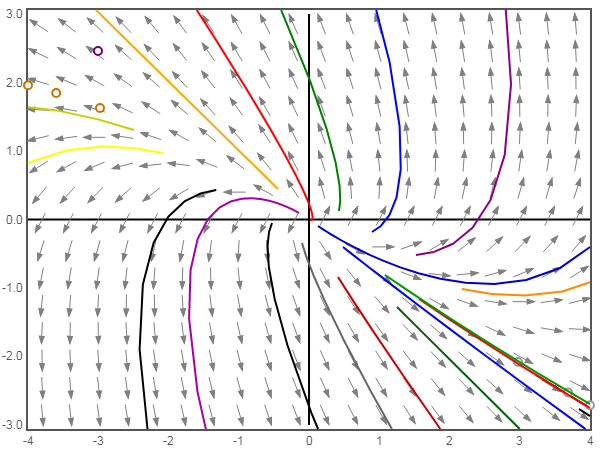
\includegraphics[width=\linewidth]{images/7.8-1.png}
\end{image}%
The particular solution to the IVP is given by:%
\begin{image}{0}{1}{0}%
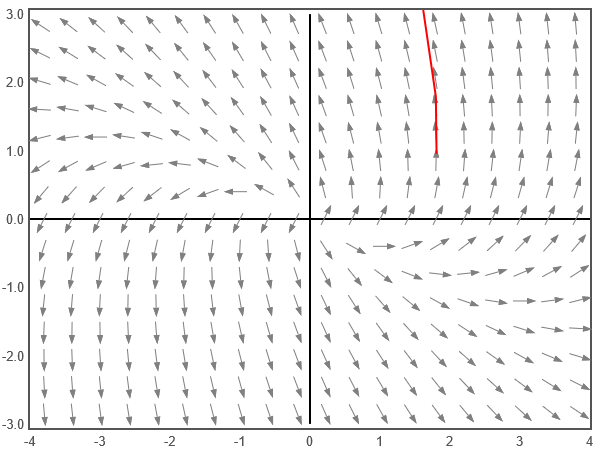
\includegraphics[width=\linewidth]{images/7.8-1b.png}
\end{image}%
\end{example}
In the case when we get repeated negative eigenvalues. Then we classify the equilibrium solution as an \terminology{asymptotically stable improper node}. The solutions look like almost spirals going towards the origin.%
\end{subsectionptx}
%
%
\typeout{************************************************}
\typeout{Subsection 5.7.2 Systems with a zero eigenvalue (\(\det A=0 \))}
\typeout{************************************************}
%
\begin{subsectionptx}{Systems with a zero eigenvalue (\(\det A=0 \))}{}{Systems with a zero eigenvalue (\(\det A=0 \))}{}{}{g:subsection:id521417}
Recall that when \(\det A=0\) then by \hyperref[x:theorem:thmlinalg1]{Theorem~{\xreffont\ref{x:theorem:thmlinalg1}}}, we must have infinitely many equilibrium solutions. Note that in all examples we've worked with so far, the only equilibrium solution was the trivial equilibrium solution, which means we've only worked with systems where \(\det A\neq0\). It turns out that when \(\det A=0\) then there will always exist be a zero eigenvalue, say%
\begin{equation*}
\lambda_{1}=0.
\end{equation*}
%
\begin{proposition}{}{}{x:proposition:prop-5-7-1}%
Let \(A\) be a \(2\times 2\) matrix. If \(\det A=0\), then one of the eigenvalues will be \(0\).%
\end{proposition}
\begin{proof}{}{g:proof:id521426}
We leave this as an exercise.%
\end{proof}
Now when \(\det A=0\), then%
\begin{equation*}
\lambda_{1}=0\,\,\,\,\,\lambda_{1}=\text{ some other real number},
\end{equation*}
with corresponding eigenvectors \(\mathbf{v}_{1}\) and \(\mathbf{v}_{2}\), respectively. Let's assume for now that \(\lambda_{2}\) is distinct from \(\lambda_{1}\). Then we are back at the distinct, real eigenvalue case, and hence everything from \hyperref[x:section:ch5-4]{Section~{\xreffont\ref{x:section:ch5-4}}} still hold. Thus the general solution to%
\begin{equation*}
\mathbf{x}^{\prime}=A\mathbf{x}
\end{equation*}
is given by%
\begin{align*}
\mathbf{x}(t) \amp =c_{1}e^{\lambda_{1}t}\mathbf{v}_{1}+c_{2}e^{\lambda_{2}t}\mathbf{v}_{2}\\
\amp =c_{1}e^{0}\mathbf{v}_{1}+c_{2}e^{\lambda_{2}t}\mathbf{v}_{2}\\
\amp =c_{1}\mathbf{v}_{1}+c_{2}e^{\lambda_{2}t}\mathbf{v}_{2}.
\end{align*}
%
\par
The only main difference is that the Phase portrait will look different, since now there are infinitely many equilibrium solutions for this system. In fact, all solutions are either straight line solutions, or are equilibrium solutions. We describe this case, in the following example.%
\begin{example}{}{x:example:ex-5-7-2}%
Consider the system%
\begin{equation*}
\frac{d\mathbf{x}}{dt}=\left(\begin{array}{cc}
-3 \amp 1\\
3 \amp -1
\end{array}\right)\mathbf{x}.
\end{equation*}
Find the general solution and draw its Phase portrait.%
\par
\terminology{Solution:}%
\par
Note \(\det A=0\) then this will always tell us that one of the eigenvalues is \(\lambda_{1}=0\). One can easily find that%
\begin{equation*}
\lambda_{2}=-4.
\end{equation*}
After some work,  one obtains that%
\begin{enumerate}
\item{}The eigenvalue \(\lambda_{1}=0\) has all eigenvectors on the line \(x_{2}=3x_{1}\), so choose \(\mathbf{v}_{1}=\left(\begin{array}{c}
1\\
3
\end{array}\right)\).%
\item{}The eigenvalue \(\lambda_{1}=-4\) has all eigenvectrs on the line \(x_{1}=-x_{2}\), so choose \(\mathbf{v}_{2}=\left(\begin{array}{c}
-1\\
1
\end{array}\right)\).%
\end{enumerate}
%
\par
The general solution is given by%
\begin{align*}
\mathbf{x}(t) \amp =  c_{1}e^{0t}\left(\begin{array}{c}
1\\
3
\end{array}\right)+c_{2}e^{-4t}\left(\begin{array}{c}
-1\\
1
\end{array}\right)\\
\amp =  c_{1}\left(\begin{array}{c}
1\\
3
\end{array}\right)+c_{2}e^{-4t}\left(\begin{array}{c}
-1\\
1
\end{array}\right).
\end{align*}
%
\par
\terminology{Draw the Phase portrait:}%
\par
Where are the infinite equilibrium solutions? The line corresponding to the eigenvectors for the zero eigenvalue is where all the equilibrium solutions are located. All other solutions are straight-solutions that either source out or sink in (depending on the sign of \(\lambda_{2}\)). In this example, all the straight-line solutions point inwards because \(\lambda_{2}=-4\). The slope of the straight-line solutions are given by direction of the eigenvector \(\mathbf{v}_{2}=\left(\begin{array}{c}
-1\\
1
\end{array}\right)\).%
\par
Here is a graph of the Phase portrait:%
\begin{image}{0}{1}{0}%
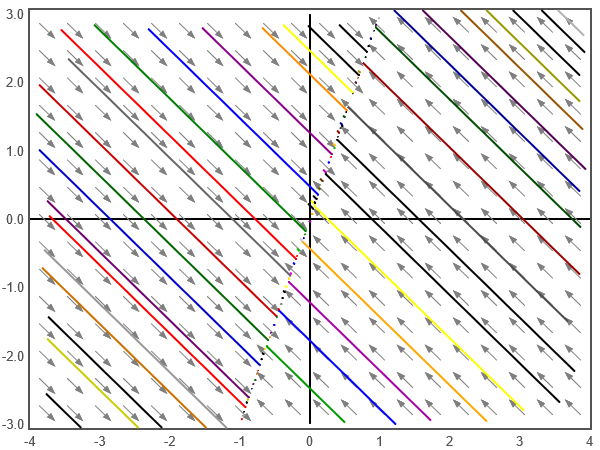
\includegraphics[width=\linewidth]{images/7.8-1c.png}
\end{image}%
\end{example}
\begin{example}{}{g:example:id521602}%
Draw a sketch of the solution to the following IVP:%
\begin{equation*}
\frac{d\mathbf{x}}{dt}=\left(\begin{array}{cc}
-3 \amp 1\\
3 \amp -1
\end{array}\right)\mathbf{x},\,\,\,\,\,\mathbf{x}(0)=\left(\begin{array}{c}
-1\\
1
\end{array}\right).
\end{equation*}
%
\par
\terminology{Solution:}%
\par
Using the previous \hyperref[x:example:ex-5-7-2]{Example~{\xreffont\ref{x:example:ex-5-7-2}}}, we have%
\begin{image}{0}{1}{0}%
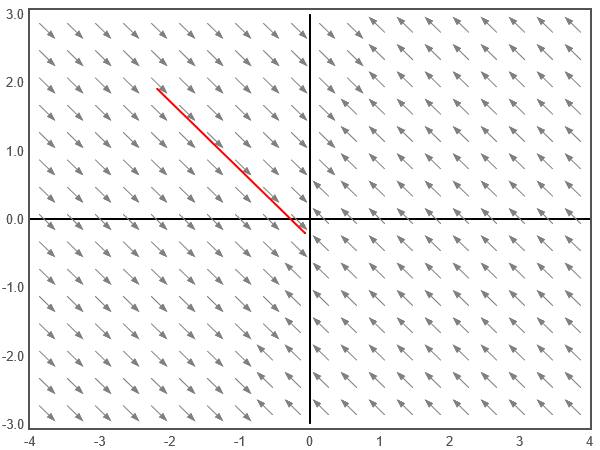
\includegraphics[width=\linewidth]{images/7.8-1d.png}
\end{image}%
\end{example}
\end{subsectionptx}
\end{sectionptx}
\end{chapterptx}
%
%
\typeout{************************************************}
\typeout{Chapter 6 The Laplace Transform}
\typeout{************************************************}
%
\begin{chapterptx}{The Laplace Transform}{}{The Laplace Transform}{}{}{x:chapter:ch6}
%
%
\typeout{************************************************}
\typeout{Section 6.1 The definition of the Laplace transform}
\typeout{************************************************}
%
\begin{sectionptx}{The definition of the Laplace transform}{}{The definition of the Laplace transform}{}{}{x:section:ch6-1}
In this section, we define \(\mathcal{L}\), the Laplace transform, which is one of the major mathematical tools of engineering and the mathematics of physical systems. Before defining the Laplace Transform we review \terminology{improper integrals},         since its definition depends on it.%
\begin{assemblage}{}{g:assemblage:id521646}%
An improper integral with an infinite limit of integration is shorthand for the limit%
\begin{equation*}
\int_{a}^{\infty}f(t)dt=\lim_{B\to\infty}\int_{a}^{B}f(t)dt.
\end{equation*}
%
\end{assemblage}
If the limit converges then the improper integral converges. If the limit diverges, then the improper integral diverges.%
\par
We also need to be able to integrate through simple discontinuities in functions that change definition.%
\begin{definition}{}{g:definition:id521655}%
A function \(f\) is \terminology{piecewise continuous} on \(\alpha\leq t\leq\beta\) if it is continuous there except for a finite number of jump (or removable) discontinuities.%
\end{definition}
\begin{example}{}{g:example:id521667}%
Are the following functions piecewise continutions?%
\begin{equation*}
f(t)=\begin{cases}
t^{2} \amp 0\leq t\leq1\\
1 \amp 1\lt t\leq2\\
4-t \amp 2\lt t\leq3
\end{cases}
\end{equation*}
and%
\begin{equation*}
g(t)=\begin{cases}
t^{2} \amp 0\leq t\leq1\\
(t-1)^{-1} \amp 1\lt t\leq2\\
1 \amp 2\lt t\leq3.
\end{cases}
\end{equation*}
%
\par
Solution: Sketch the graphs \(f(t)\) is piecewise continuous since it only has a jump discontinuity. \(g(t)\) is \emph{not} since it has a discontinuity that is not jump or removable.%
\end{example}
\begin{example}{Integrating piecewise functions.}{g:example:id521684}%
Consider \begin{image}{0.25}{0.5}{0.25}%
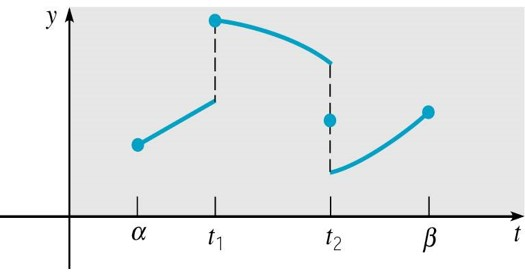
\includegraphics[width=\linewidth]{images/6.1-1.jpg}
\end{image}%
 Then%
\begin{equation*}
\int_{\alpha}^{\beta}f(t)dt=\int_{\alpha}^{t_{1}}f(t)dt+\int_{t_{1}}^{t_{2}}f(t)dt+\int_{t_{2}}^{\beta}f(t)dt.
\end{equation*}
%
\end{example}
The goal of using the Laplace transform is to change the differential equations, which have techniques of solution built on calculus, into the language of algebraic equations, which have techniques of solution built on high school algebra. The hope is that once we discover a solution to the algebraic equation, we can transform it back into a solution for the original ODE.%
\par
%
\begin{equation*}
\begin{array}{ccc}
\text{ODE Equation} \amp \overset{\mathcal{L}}{\implies} \amp \text{Algebraic Equation}\\
\amp  \amp \Downarrow\\
\text{Turn it into an ODE Solution } \amp \underset{\mathcal{L}^{-1}}{\Longleftarrow} \amp \text{Solve the Algebrac EQ}
\end{array}
\end{equation*}
Thus the Laplace transforms a function \(f(t)\) into a function \(F(s)\), which is representied symbolically as%
\begin{equation*}
f(t)\overset{\mathcal{L}}{\longrightarrow}F(s).
\end{equation*}
%
\par
Generally, a \terminology{transform} of a function \(f(t)\) turns \(f(t)\) into a different function with potentially more tractible properties. We will transform functions \(f(t)\) of \(t\) in the \terminology{time domain} into functions \(F(s)\) of \(s\) in the \terminology{frequency domain}. The use of these terms is deliberate and will become clear on further study.%
\par
We are now ready to define the transform of greatest use in the solution of linear differential equations.%
\begin{definition}{}{g:definition:id521744}%
The \terminology{Laplace transform} of \(f\) is given by%
\begin{equation*}
\mathcal{L}\left\{ f(t)\right\} =F(s)=\int_{0}^{\infty}f(t)e^{-st}dt.
\end{equation*}
We assume \(s\) is real (though in general it can be complex).%
\end{definition}
In general, we should be suspicious of integrals involving infinity as a limit of integration. Why should we believe that such an integral is likely to converge? The key observation is that the exponential function \(e^{-st}\) tends to \(0\) \emph{very quickly}. In fact exponentials dominate all polynomials, which is going to mean that the functions most commonly used in differential equations (polynomials, trig functions, and exponentials with domain restrictions) are all reasonably controlled by the exponential function \(e^{-st}\).%
\begin{assemblage}{Existence of \(\mathcal{L}\left\{ f(t)\right\} \).}{g:assemblage:id521784}%
If \(f\) is piecewise continuous for \(\left[0,a\right]\) for all \(a\) and            \(\left|f(t)\right|\leq Ke^{ct}\) for large \(t\), then \(\mathcal{L}\left[f(t)\right]=F(s)\) exists.%
\end{assemblage}
The following examples may seem cumbersome, but rest easy! After using the definition to get a feel for how the Laplace transform works, we'll develop a table of known and useful transforms and our study will be more algebraic.%
\begin{example}{}{g:example:id521841}%
Find the Laplace transform of \(f(t)=e^{9t}\), \(t\geq0\) .%
\par
Solution: We compute%
\begin{align*}
\mathcal{L}\left\{ e^{9t}\right\}  \amp =\int_{0}^{\infty}f(t)e^{-st}dt=\int_{0}^{\infty}e^{9t}e^{-st}dt\\
\amp =\int_{0}^{\infty}e^{(9-s)t}dt\\
\amp =\frac{1}{9-s}\left[e^{(9-s)t}\right]_{t=0}^{t=\infty}\\
\amp =\frac{1}{9-s}\left[\lim_{b\to\infty}e^{(9-s)b}-e^{0}\right]
\end{align*}
but since%
\begin{equation*}
\lim_{b\to\infty}e^{(9-s)b}=\begin{cases}
\infty \amp a-s>0\\
0 \amp a-s\lt 0
\end{cases}
\end{equation*}
then%
\begin{equation*}
\mathcal{L}\left\{ e^{9t}\right\} =\begin{cases}
\frac{1}{s-9} \amp s>9\\
\text{not defined} \amp s\lt 9
\end{cases}.
\end{equation*}
%
\end{example}
\begin{example}{}{g:example:id521882}%
Find the Laplace transform of \(f(t)=e^{at}\), \(t\geq0\) .%
\par
We can use the same computation as in Example 1, but change every \(9\) to an \(a\) and get%
\begin{equation*}
\mathcal{L}\left\{ e^{at}\right\} =\frac{1}{s-a}\,\,\,\,\,\,s>a.
\end{equation*}
%
\end{example}
\begin{example}{}{g:example:id521852}%
Find the Laplace transform of \(f(t)=1\), \(t\geq0\) .%
\par
Solution: Using \(a=0\) above we have that \(f(t)=e^{0\cdot t}=1\) hence we can use the formula above to get%
\begin{equation*}
\mathcal{L}\left\{ 1\right\} =\frac{1}{s}\,\,\,\,\,\,s>0.
\end{equation*}
%
\end{example}
Eventually, we'll make a table where we collect all of the Laplace transforms that we have computed, so that we don't have to redo the work everytime.%
\begin{example}{}{g:example:id521901}%
Find the Laplace transform of \(f(t)=\sin(at)\).%
\par
Solution: We compute%
\begin{align*}
\mathcal{L}\left\{ \sin at\right\} =F(s) \amp =\int_{0}^{\infty}e^{-st}\sin(at)dt\\
\amp =\lim_{B\to\infty}\int_{0}^{B}e^{-st}\sin(at)dt.
\end{align*}
Using integration by parts, we get%
\begin{align*}
u=\sin(at)\,\,\,\,\,\,\,\, \amp dv=e^{-st}dt\\
du=a\cos(at)dt\,\,\,\,\,\,\,\, \amp v=-\frac{e^{-st}}{s}
\end{align*}
so we have%
\begin{align*}
F(s) \amp =\lim_{B\to\infty}\left[\left.-\frac{e^{-st}\sin(at)}{s}\right|_{t=0}^{t=B}+\int_{0}^{B}\frac{e^{-st}}{s}a\cos(at)dt\right]\\
\amp =\lim_{B\to\infty}\left[-\frac{e^{-sB}\sin(aB)}{s}+0+\int_{0}^{B}\frac{e^{-st}}{s}a\cos(at)dt\right]\\
\amp =0+\frac{a}{s}\int_{0}^{\infty}e^{-st}\cos(at)dt.\,\,\,\,\,\,\,\,(\star)
\end{align*}
Integrating \(\int_{0}^{\infty}e^{-st}\cos(at)dt\) again we get%
\begin{align*}
u=\cos(at)\,\,\,\,\,\,\,\, \amp dv=e^{-st}dt\\
du=-a\sin(at)dt\,\,\,\,\,\,\,\, \amp v=-\frac{e^{-st}}{s}
\end{align*}
%
\begin{align*}
\int_{0}^{\infty}e^{-st}\cos(at)dt \amp =\lim_{B\to\infty}\left[\left.-\frac{e^{-st}\cos(at)}{s}\right|_{t=0}^{t=B}-\int_{0}^{B}\frac{e^{-st}}{s}a\sin(at)dt\right]\\
\amp =\lim_{B\to\infty}\left[-\frac{e^{-sB}\cos(aB)}{s}+\frac{e^{-st}}{s}-\frac{a}{s}\int_{0}^{B}\frac{e^{-st}}{s}a\sin(at)dt\right]\\
\amp =\left[0+\frac{t}{s}-\frac{a}{s}\int_{0}^{\infty}e^{-st}\sin(at)dt\right].
\end{align*}
Plugging this back into \((\star)\) we have%
\begin{align*}
F(t) \amp =\frac{a}{s}\left[\frac{1}{s}-\frac{a}{s}\int_{0}^{\infty}e^{-st}\sin(at)dt\right]\\
\amp =\frac{a}{s}\left[\frac{1}{s}-\frac{a}{s}F(s)\right]
\end{align*}
Then we can solve this equation using algebra for \(F(s)\) and get%
\begin{equation*}
F(s)=\frac{a}{s^{2}+a^{2}},\,\,\,\,s>0.
\end{equation*}
%
\end{example}
\begin{assemblage}{Properties of the Laplace Transform: Linearity.}{g:assemblage:id521975}%
If \(f,g\) are two function where \(\mathcal{L}\) exists for \(s>a_{1}\) and \(s>a_{2}\), respectively, Then%
\begin{equation*}
\mathcal{L}\left\{ f(t)\pm g(t)\right\} =\mathcal{L}\left\{ f(t))\right\} \pm\mathcal{L}\left\{ g(t)\right\} ,\,\,\,s>\max\left\{ a_{1},a_{2}\right\} ,
\end{equation*}
and We have for \(c\in\mathbb{R}\),%
\begin{equation*}
\mathcal{L}\left\{ cf(t))\right\} =c\mathcal{L}\left\{ f(t))\right\} .
\end{equation*}
%
\end{assemblage}
\begin{example}{}{g:example:id522004}%
Find the Laplace transform of \(f(t)=7-e^{2t}+4\sin(3t)\).%
\par
Solution: Using what we have computed we get%
\begin{align*}
\mathcal{L}\left\{ 7-e^{-5t}+4\sin(3t)\right\}  \amp =\mathcal{L}\left\{ 7\right\} -\mathcal{L}\left\{ e^{(-5)t}\right\} +4\mathcal{L}\left\{ \sin(3t)\right\} \\
\amp =\frac{7}{s}-\frac{1}{s-(-5)}+4\cdot\frac{3}{s^{2}+9}\\
\amp =\frac{7}{s}-\frac{1}{s+5}+\frac{12}{s^{2}+9}.\,\,\,\,\,s>0
\end{align*}
%
\end{example}
\end{sectionptx}
%
%
\typeout{************************************************}
\typeout{Section 6.2 The Laplace Transform and Initial Value Problems}
\typeout{************************************************}
%
\begin{sectionptx}{The Laplace Transform and Initial Value Problems}{}{The Laplace Transform and Initial Value Problems}{}{}{x:section:ch6-2}
\begin{introduction}{}%
In this section we will show the connection between ODEs with given initial value conditions and Laplace Transforms. Recall that our previous methods for approaching IVPs involve solving first a homogeneous equation and then using another method, such as undertermined coefficients, to find a particular solution. Using the Laplace transform, we will be able to do this all at once.%
\par
First, we need to look at how the Laplace transform acts on derivatives.%
\begin{theorem}{Laplace transform of \(\frac{df}{dt}\).}{}{x:theorem:thm-Lapl1}%
Suppose \(f\) has a Laplace transform \(\mathcal{L}\left\{ f\right\} = F(s) \) and is controlled by some exponential \(Ke^at\). Then the Laplace transform of \(f^{\prime}\) is given by%
\begin{equation*}
\mathcal{L}\left\{ f^{\prime}(t)\right\} =s\mathcal{L}\left\{ f(t)\right\} -f(0).
\end{equation*}
%
\end{theorem}
\begin{proof}{}{g:proof:id522066}
Let%
\begin{equation*}
\mathcal{L}\left\{ f^{\prime}(t)\right\} =\lim_{B\to\infty}\int_{0}^{B}f^{\prime}(t)e^{-st}dt
\end{equation*}
and we use integration by parts%
\begin{align*}
u \amp=e^{-st} \amp \,\,\,\,\,\,\,\,\,\,\,dv=f^{\prime}(t)dt\\
du \amp =-se^{-st}dt \amp \,\,\,\,\,\,\,\,\,\,\,v=f(t)
\end{align*}
we have%
\begin{align*}
\mathcal{L}\left\{ f^{\prime}(t)\right\}  \amp =\lim_{B\to\infty}\left[f(t)e^{-st}\right]_{t=0}^{t=B}+\int_{0}^{B}f(t)se^{-st}dt\\
\amp =\left[0-f(0)\right]+s\int_{0}^{\infty}f(t)e^{-st}dt\\
\amp =-f(0)+s\mathcal{L}\left\{ f(t)\right\} ,
\end{align*}
here we use the condition from \hyperref[x:theorem:thm-Lapl1]{Theorem~{\xreffont\ref{x:theorem:thm-Lapl1}}} that says \(\left|f(t)\right|\leq Ke^{at}\) for \(t\geq M\) which implies that \(\lim_{B\to\infty}f(B)e^{-sB}=0\) when \(s>a\).  Rearranging gives us the desired result.%
\end{proof}
\begin{corollary}{}{}{x:corollary:chp6-cor1}%
Suppose \(f,f^{\prime},\dots,f^{(n)}\) are nice functions that have Laplace transforms, then%
\begin{equation*}
\mathcal{L}\left\{ f^{(n)}(t)\right\} =s^{n}\mathcal{L}\left\{ f(t)\right\} -s^{n-1}f(0)\cdots-sf^{(n-2)}(0)-f^{(n-1)}(0).
\end{equation*}
%
\end{corollary}
\begin{example}{}{g:example:id522126}%
\(\mathcal{L}\left\{ f^{\prime\prime}(t)\right\} =s^{2}\mathcal{L}\left\{ f(t)\right\} -sf(0)-f^{\prime}(0)\). \(\mathcal{L}\left\{ f^{\prime\prime\prime}(t)\right\} =s^{3}\mathcal{L}\left\{ f(t)\right\} -s^{2}f(0)-sf^{\prime}(0)-f^{\prime\prime}(0)\).\end{example}
\end{introduction}%
%
%
\typeout{************************************************}
\typeout{Subsection 6.2.1 Inverse Laplace Transforms}
\typeout{************************************************}
%
\begin{subsectionptx}{Inverse Laplace Transforms}{}{Inverse Laplace Transforms}{}{}{g:subsection:id522152}
The Inverse Laplace transform \(\mathcal{L}^{-1}\) is the function that satisfies \(\mathcal{L}^{-1}\left\{ \mathcal{L}\left[f\right]\right\} =f\). In other words,%
\begin{equation*}
\mathcal{L}^{-1}\left\{ F\right\} =f\iff\mathcal{L}\left\{ f\right\} =F.
\end{equation*}
%
\begin{assemblage}{Some example inverse transforms.}{g:assemblage:id522141}%
%
\begin{equation*}
\mathcal{L}^{-1}\left\{ \frac{1}{s}\right\} =1\text{.}
\end{equation*}
%
\begin{equation*}
\mathcal{L}^{-1}\left\{ \frac{1}{s-1}\right\} =e^{t}
\end{equation*}
%
\begin{equation*}
\mathcal{L}^{-1}\left\{ \frac{10}{s+1}\right\} =10\mathcal{L}^{-1}\left\{ \frac{1}{s-(-1)}\right\} =10e^{-t}\text{.}
\end{equation*}
%
\begin{equation*}
\mathcal{L}^{-1}\left\{ \frac{6}{s^{2}+7}\right\} =6\mathcal{L}^{-1}\left\{ \frac{1}{s^{2}+\left(\sqrt{7}\right)^{2}}\right\} =\frac{6}{\sqrt{7}}\mathcal{L}^{-1}\left\{ \frac{\sqrt{7}}{s^{2}+\left(\sqrt{7}\right)^{2}}\right\} =\frac{6}{\sqrt{7}}\sin\left(\sqrt{7}t\right)\text{.}
\end{equation*}
%
\end{assemblage}
In general,%
\begin{equation*}
\mathcal{L}^{-1}\left\{ \frac{1}{s-a}\right\} =e^{at}.
\end{equation*}
%
\par
We'll typically have rational functions for which we need to find inverse transforms. As an example, let's compute \(\mathcal{L}^{-1}\left\{ \frac{4}{\left(s-1\right)\left(s+1\right)}\right\} \). Whenever we have linear or irreducible quadratic factors in the denominator, we need to use partial fractions:%
\begin{equation*}
\frac{4}{\left(s-1\right)\left(s+1\right)}=\frac{A}{\left(s-1\right)}+\frac{B}{\left(s+1\right)},
\end{equation*}
hence%
\begin{align*}
4 \amp =A\left(s+1\right)+B\left(s-1\right),\\
0\cdot s+4 \amp =\left(A+B\right)s+\left(A-B\right)
\end{align*}
so that%
\begin{align*}
A+B \amp =0\\\\
A-B \amp =4
\end{align*}
and get \(A=2,B-2\). Thus%
\begin{equation*}
\frac{4}{\left(s-1\right)\left(s+1\right)}=\frac{2}{s-1}-\frac{2}{s+1}.
\end{equation*}
Therefore:%
\begin{align*}
\mathcal{L}^{-1}\left\{ \frac{4}{\left(s-1\right)\left(s+1\right)}\right\}  \amp =\mathcal{L}^{-1}\left\{ \frac{4}{\left(s-1\right)\left(s+1\right)}\right\}\\
\amp =\mathcal{L}^{-1}\left\{ \frac{2}{s-1}\right\} -\mathcal{L}^{-1}\left\{ \frac{2}{s+1}\right\} \\
\amp =2e^{t}-2e^{-t}.
\end{align*}
%
\begin{example}{}{g:example:id522225}%
Find \(\mathcal{L}^{-1}\left\{ \frac{6}{s\left(s+4\right)}\right\} \).%
\par
First%
\begin{equation*}
\frac{6}{s\left(s+4\right)}=\frac{A}{s}+\frac{B}{\left(s+4\right)}
\end{equation*}
so that%
\begin{equation*}
6=A\left(s+4\right)+Bs
\end{equation*}
or%
\begin{equation*}
0s+6=\left(A+B\right)s+4A
\end{equation*}
and get%
\begin{align*}
\end{align*}
so that \(A=-\frac{3}{2}\) and \(B=\frac{3}{2}\) hence%
\begin{align*}
\mathcal{L}^{-1}\left\{ \frac{6}{s\left(s+4\right)}\right\}  \amp =\mathcal{L}^{-1}\left\{ \frac{3/2}{s}+\frac{-3/2}{\left(s+4\right)}\right\} \\
\amp =\frac{3}{2}\mathcal{L}^{-1}\left\{ \frac{1}{s}\right\} -\frac{3}{2}\mathcal{L}\left\{ \frac{1}{\left(s+4\right)}\right\} \\
\amp =\frac{3}{2}\cdot1-\frac{3}{2}\mathcal{L}\left\{ \frac{1}{s-(-4)}\right\} \\
\amp =\frac{3}{2}\cdot1-\frac{3}{2}e^{-4t}
\end{align*}
%
\end{example}
\end{subsectionptx}
%
%
\typeout{************************************************}
\typeout{Subsection 6.2.2 Solving IVPs using Laplace Transforms}
\typeout{************************************************}
%
\begin{subsectionptx}{Solving IVPs using Laplace Transforms}{}{Solving IVPs using Laplace Transforms}{}{}{g:subsection:id522258}
We'll now combine the partial fraction technique with the Laplace transform to solve first order IVPS.%
\begin{example}{}{g:example:id522249}%
Solve%
\begin{equation*}
y^{\prime}=y-4e^{-t},\,\,\,y(0)=1
\end{equation*}
using Laplace transforms.%
\par
Step 1: Find the Laplace Transform of the ODE (The going forwards part):%
\begin{align*}
\mathcal{L}\left\{ y^{\prime}\right\} =\mathcal{L}\left\{ y\right\} -4\mathcal{L}\left\{ e^{-t}\right\}  \amp \iff s\mathcal{L}\left\{ y\right\} -y(0)=\mathcal{L}\left\{ y\right\} -4\frac{1}{s+1}\\
\amp \iff s\mathcal{L}\left\{ y\right\} -1=\mathcal{L}\left\{ y\right\} -4\frac{1}{s+1}.
\end{align*}
%
\par
Step 2: Solve for \(\mathcal{L}\left\{ y\right\} \) using algebra: and get%
\begin{equation*}
\mathcal{L}\left\{ y\right\} =\frac{1}{s-1}-\frac{4}{\left(s-1\right)\left(s+1\right)}.
\end{equation*}
%
\par
Step 3: We want to go backwards and invert this. But first let's do partial fractions:%
\begin{equation*}
\frac{4}{\left(s-1\right)\left(s+1\right)}=\frac{A}{\left(s-1\right)}+\frac{B}{\left(s+1\right)},
\end{equation*}
hence%
\begin{align*}
4 \amp =A\left(s+1\right)+B\left(s-1\right),\\
0\cdot s+4 \amp =\left(A+B\right)s+\left(A-B\right)
\end{align*}
so that%
\begin{align*}
A+B \amp =0\\
A-B \amp =4
\end{align*}
and get \(A=2,B=-2\). Thus%
\begin{equation*}
\frac{4}{\left(s-1\right)\left(s+1\right)}=\frac{2}{s-1}-\frac{2}{s+1}.
\end{equation*}
%
\par
Step 4: Use the inverse Laplace transform to get%
\begin{align*}
y=\mathcal{L}^{-1}\left\{ \mathcal{L}\left\{ y\right\} \right\}  \amp =\mathcal{L}^{-1}\left\{ \frac{1}{s-1}\right\} -\mathcal{L}^{-1}\left\{ \frac{4}{\left(s-1\right)\left(s+1\right)}\right\} \\
\amp =\mathcal{L}^{-1}\left\{ \frac{1}{s-1}\right\} -\left(\mathcal{L}^{-1}\left\{ \frac{2}{s-1}\right\} -\mathcal{L}^{-1}\left\{ \frac{2}{s+1}\right\} \right)\\
\amp =e^{t}-\mathcal{L}^{-1}\left\{ \frac{2}{s-1}\right\} +\mathcal{L}^{-1}\left\{ \frac{2}{s+1}\right\} \\
\amp =e^{t}-2e^{t}+2e^{-t}\\
\amp =-e^{t}+2e^{-t}.
\end{align*}
%
\end{example}
\begin{example}{}{g:example:id522310}%
Solve%
\begin{equation*}
y^{\prime}+4y=6,\,\,\,y^{\prime}(0)=0
\end{equation*}
using Laplace transforms.%
\par
Step 1: Find the Laplace Transform of the ODE (The going forwards part):%
\begin{align*}
\mathcal{L}\left\{ y^{\prime}\right\} +4\mathcal{L}\left\{ y\right\} =\mathcal{L}\left\{ 6\right\}  \amp \iff s\mathcal{L}\left\{ y\right\} -y(0)+4\mathcal{L}\left\{ y\right\} =\frac{6}{s}
\end{align*}
%
\par
Step 2: Solve for \(\mathcal{L}\left\{ y\right\} \) using algebra: and get%
\begin{equation*}
\mathcal{L}\left\{ y\right\} =\frac{6}{s\left(s+4\right)}.
\end{equation*}
%
\par
Step 3: Partial Fractions (We did this already)%
\begin{equation*}
\frac{6}{s\left(s+4\right)}=\frac{3/2}{s}+\frac{-3/2}{\left(s+4\right)}
\end{equation*}
%
\par
Step 4: Use the inverse Laplace transform to get%
\begin{align*}
y=\mathcal{L}^{-1}\left\{ \mathcal{L}\left\{ y\right\} \right\}  \amp =\mathcal{L}^{-1}\left\{ \frac{3/2}{s}+\frac{-3/2}{\left(s+4\right)}\right\} \\
\amp =\frac{3}{2}\mathcal{L}^{-1}\left\{ \frac{1}{s}\right\} -\frac{3}{2}\mathcal{L}\left\{ \frac{1}{\left(s+4\right)}\right\} \\
\amp =\frac{3}{2}\cdot1-\frac{3}{2}\mathcal{L}\left\{ \frac{1}{s-(-4)}\right\} \\
\amp =\frac{3}{2}\cdot1-\frac{3}{2}e^{-4t}
\end{align*}
%
\end{example}
\end{subsectionptx}
\end{sectionptx}
%
%
\typeout{************************************************}
\typeout{Section 6.3 Solutions to higher order IVPs}
\typeout{************************************************}
%
\begin{sectionptx}{Solutions to higher order IVPs}{}{Solutions to higher order IVPs}{}{}{x:section:ch6-3}
\begin{introduction}{}%
Recall the folloing consequence of the Laplace transform of a derivative:%
\begin{corollary}{}{}{g:corollary:id522360}%
Suppose \(f,f^{\prime},\dots,f^{(n)}\) are nice functions that have Laplace transforms, then%
\begin{equation*}
\mathcal{L}\left\{ f^{(n)}(t)\right\} =s^{n}\mathcal{L}\left\{ f(t)\right\} -s^{n-1}f(0)\cdots-sf^{(n-2)}(0)-f^{(n-1)}(0).
\end{equation*}
%
\end{corollary}
 For example, \begin{assemblage}{}{g:assemblage:id522394}%
%
\begin{enumerate}
\item{}\(\mathcal{L}\left\{ f^{\prime\prime}(t)\right\} =s^{2}\mathcal{L}\left\{ f(t)\right\} -sf(0)-f^{\prime}(0)\).%
\item{}\(\mathcal{L}\left\{ f^{\prime\prime\prime}(t)\right\} =s^{3}\mathcal{L}\left\{ f(t)\right\} -s^{2}f(0)-sf^{\prime}(0)-f^{\prime\prime}(0)\).%
\end{enumerate}
%
\end{assemblage}
\end{introduction}%
%
%
\typeout{************************************************}
\typeout{Subsection 6.3.1 Laplace Transforms Table}
\typeout{************************************************}
%
\begin{subsectionptx}{Laplace Transforms Table}{}{Laplace Transforms Table}{}{}{x:subsection:laplace-table}
Typically, we use a table to compute Laplace transforms and inverse transforms. The examples below refer to the transforms listed on the following table.%
\begin{assemblage}{}{g:assemblage:id522411}%
%
\begin{equation*}
\begin{array}{l|l}
f(t) = \mathcal{L}\inv\{F(s)\} \amp F(s) = \mathcal{L}\{f(t)\} \\[4pt] \hline
\text{1. } 1 \amp \frac{1}{s}, \hspace{.2in} s > 0 \\[4pt]
\text{2. } e^{at} \amp \frac{1}{s-a}, \hspace{.2in} s > a \\[4pt]
\text{3. } t^n, n=\text{ positive integer} \amp \frac{n!}{s^{n+1}}, \hspace{.2in} s > 0 \\[4pt]
\text{4. } t^p, p > -1 \amp \frac{\Gamma(p+1)}{s^{p+1}}, \hspace{.2in} s > 0 \\[4pt]
\text{5. } \sin at \amp \frac{a}{s^2 + a^2}, \hspace{.2in} s > 0 \\[4pt]
\text{6. } \cos at \amp \frac{s}{s^2 + a^2}, \hspace{.2in} s > 0 \\[4pt]
\text{7. } \sinh at \amp \frac{a}{s^2 - a^2}, \hspace{.2in} s > \abs{a} \\[4pt]
\text{8. } \cosh at \amp \frac{s}{s^2 - a^2}, \hspace{.2in} s > \abs{a} \\[4pt]
\text{9. } e^{at} \sin bt \amp \frac{b}{(s-a)^2 + b^2}, \hspace{.2in} s > a\\[4pt]
\text{10. } e^{at} \cos bt \amp \frac{s - a}{(s-a)^2 + b^2}, \hspace{.2in} s > a \\[4pt]
\text{11. } t^n e^{at}, n=\text{ positive integer} \amp \frac{n!}{(s-a)^{n+1}}, \hspace{.2in} s > a
\end{array}
\end{equation*}
%
\end{assemblage}
\end{subsectionptx}
%
%
\typeout{************************************************}
\typeout{Subsection 6.3.2 Partial fractions}
\typeout{************************************************}
%
\begin{subsectionptx}{Partial fractions}{}{Partial fractions}{}{}{g:subsection:id522413}
The essential step in computing an inverse Laplace transform is separating the function \(F\) into pieces that we can apply the inverse transform to. This is typically done via partial fractions. Make sure you first factor the denominator as much as possible%
\begin{enumerate}
\item{}The correct form of the partial fractions is%
\begin{equation*}
\frac{5s}{\left(s-1\right)\left(s^{2}+1\right)}=\frac{A}{s-1}+\frac{Bs+C}{s^{2}+1}
\end{equation*}
%
\item{}The correct form of the partial fractions is%
\begin{equation*}
\frac{6s+1}{\left(s-1\right)^{3}\left(s^{2}+3\right)}=\frac{A}{s-1}+\frac{B}{\left(s-1\right)^{2}}+\frac{C}{\left(s-1\right)^{3}}+\frac{Ds+E}{s^{2}+3}
\end{equation*}
%
\item{}The correct form of the partial fractions is%
\begin{equation*}
\frac{9s-1}{s\left(s^{2}+9\right)\left(s-5\right)}=\frac{A}{s}+\frac{Bs+C}{s^{2}+9}+\frac{D}{s-5}
\end{equation*}
%
\item{}The correct form of the partial fractions is%
\begin{equation*}
\frac{s^{2}+s-1}{\left(s^{2}+1\right)^{3}\left(s-1\right)}=\frac{As+B}{s^{2}+1}+\frac{Cs+D}{\left(s^{2}+1\right)^{2}}+\frac{Es+F}{\left(s^{2}+1\right)^{3}}+\frac{G}{s-1}.
\end{equation*}
%
\item{}The correct form of the partial fractions is%
\begin{align*}
\frac{9s+1}{\left(s^{4}+1\right)\left(s^{2}+2s+10\right)s^{2}} \amp =\frac{As^{3}+Bs^{2}+Cs+D}{s^{4}+1}+\frac{Es+F}{s^{2}+2s+10}.\\
\amp +\frac{G}{s}+\frac{H}{s^{2}}.
\end{align*}
%
\end{enumerate}
%
\end{subsectionptx}
%
%
\typeout{************************************************}
\typeout{Subsection 6.3.3 Inverse Laplace Transforms}
\typeout{************************************************}
%
\begin{subsectionptx}{Inverse Laplace Transforms}{}{Inverse Laplace Transforms}{}{}{g:subsection:id520216}
\begin{example}{}{g:example:id520228}%
Find the inverse transform of \(F(s)=\frac{1}{s^{4}+s^{2}}\)%
\par
First let's do partial fractions:%
\begin{equation*}
\frac{1}{s^{2}\left(s^{2}+1\right)}=\frac{A}{s}+\frac{B}{s^{2}}+\frac{Cs+D}{s^{2}+1}
\end{equation*}
hence%
\begin{equation*}
1=As\left(s^{2}+1\right)+B\left(s^{2}+1\right)+\left(Cs+D\right)s^{2}
\end{equation*}
so that%
\begin{equation*}
0s^{3}+0s^{2}+0s+1=\left(A+C\right)s^{3}+\left(B+D\right)s^{2}+As+B
\end{equation*}
and get the equations%
\begin{align*}
\end{align*}
and get \(B=1,A=0,C=0,D=-1\). Thus%
\begin{equation*}
\frac{1}{s^{2}\left(s^{2}+1\right)}=\frac{1}{s^{2}}-\frac{1}{s^{2}+1}.
\end{equation*}
%
\par
Using Formulas \(3\) and \(5\) in the Laplace Trasform table:%
\begin{equation*}
\mathcal{L}\left\{ t^{n}\right\} =\frac{n!}{s^{n+1}},\,\,\,\mathcal{L}\left\{ \sin(at)\right\} =\frac{a}{s^{2}+a^{2}}.
\end{equation*}
Use get the inverse Laplace transform:%
\begin{align*}
\mathcal{L}^{-1}\left\{ F(s)\right\}  \amp =\mathcal{L}^{-1}\left\{ \frac{1}{s^{2}}\right\} -\mathcal{L}^{-1}\left\{ \frac{1}{s^{2}+1}\right\} \\
\amp =t-\sin t,
\end{align*}
%
\end{example}
\begin{example}{}{g:example:id520239}%
(Harder) Find the inverse transform of \(F(s)=\frac{1-2s}{s^{2}+4s+5}\). Note that we can't factor \(s^{2}+4s+5\) with real roots, thus we will complete the square.%
\par
\alert{Completing the Square:} Suppose we have \(s^{2}+bs+c\), then the trick is to ADD\slash{}SUBTRACT \(\left(\frac{b}{2}\right)^{2}\), and the polynomials will become \(s^{2}+bs+c=\left(s+\frac{b}{2}\right)^{2}-\left(\frac{b}{2}\right)^{2}+c\). To complete the square for \(s^{2}+4s+5\): Then \(b=4\) hence we add\slash{}subtract \(\left(\frac{b}{2}\right)^{2}=\left(\frac{4}{2}\right)^{2}=4\). Thus%
\begin{align*}
s^{2}+4s+5 \amp =s^{2}+4s+4+\left(-4+5\right)\\
\amp =\left(s+2\right)^{2}+1
\end{align*}
%
\par
Going back to the problem of find the Laplace Transform we have that%
\begin{align*}
F(s) \amp =\frac{1-2s}{s^{2}+4s+5}=\frac{1-2s}{\left(s+2\right)^{2}+1}
\end{align*}
and looking at Formulas 9 and 10 from the Laplace trasnform table:%
\begin{equation*}
\mathcal{L}\left\{ e^{at}\sin bt\right\} =\frac{b}{(s-a)^{2}+b^{2}}\text{ and }\mathcal{L}\left\{ e^{at}\cos bt\right\} =\frac{s-a}{(s-a)^{2}+b^{2}}.
\end{equation*}
We can apply these by separating \(F(s)\) into pieces like this:=%
\begin{align*}
\mathcal{L}^{-1}\left\{ F(s)\right\}  \amp =\mathcal{L}^{-1}\left\{ \frac{1-2s}{\left(s+2\right)^{2}+1}\right\} \\
\amp =\mathcal{L}^{-1}\left\{ \frac{-2\left(s+2\right)}{\left(s+2\right)^{2}+1}\right\} +\mathcal{L}^{-1}\left\{ \frac{\boldsymbol{+4}+1}{\left(s+2\right)^{2}+1}\right\} \\
\amp =-2\mathcal{L}^{-1}\left\{ \frac{\left(s-\left(-2\right)\right)}{\left(s-\left(-2\right)\right)^{2}+1}\right\} +5\mathcal{L}^{-1}\left\{ \frac{1}{\left(s+2\right)^{2}+1}\right\} \\
\amp =-2e^{-2t}\cos t+5e^{-2t}\sin t.
\end{align*}
%
\end{example}
\begin{example}{}{g:example:id524654}%
Find the inverse transform of \(F(s)=\frac{2s-8}{s^{2}-4s+5}\).%
\par
Note that we can't factor \(s^{2}-4s+5\) with real roots, thus we will complete the square.%
\par
\alert{Completing the square:} Suppose we have \(s^{2}+bs+c\), then the trick is to ADD\slash{}SUBTRACT \(\left(\frac{b}{2}\right)^{2}\), and the polynomials will become \(s^{2}+bs+c=\left(s+\frac{b}{2}\right)^{2}-\left(\frac{b}{2}\right)^{2}+c\). To complete the square for \(s^{2}-4s+5\): Then \(b=-4\) hence we add\slash{}subtract \(\left(\frac{b}{2}\right)^{2}=\left(\frac{-4}{2}\right)^{2}=4\). Thus%
\begin{align*}
s^{2}-4s+5 \amp =s^{2}-4s+4+1\\
\amp =\left(s-2\right)^{2}+1
\end{align*}
%
\par
Going back to the problem of find the Laplace Transform we have that%
\begin{align*}
F(s) \amp =\frac{2s-8}{\left(s-2\right)^{2}+1}=\frac{2\left(s-2\right)}{\left(s-2\right)^{2}+1}-4\frac{1}{\left(s-2\right)^{2}+1}
\end{align*}
We can apply these by separating \(F(s)\) into pieces like this:=%
\begin{align*}
\mathcal{L}^{-1}\left\{ F(s)\right\}  \amp =\mathcal{L}^{-1}\left\{ \frac{2s-8}{\left(s-2\right)^{2}+1}\right\} \\
\amp =\mathcal{L}^{-1}\left\{ \frac{2\left(s-2\right)}{\left(s-2\right)^{2}+1}\right\} -4\mathcal{L}^{-1}\left\{ \frac{1}{\left(s-2\right)^{2}+1}\right\} \\
\amp =2e^{2t}\cos t-4e^{2t}\sin t
\end{align*}
%
\end{example}
\begin{example}{}{g:example:id524759}%
Find the inverse transform of \(F(s)=\frac{2s-3}{s^{2}-4}\).%
\par
Notice that this one looks like Formulas 7 and 8 from the Table of Laplace Transforms:%
\begin{equation*}
\mathcal{L}\left\{ \sinh(at)\right\} =\frac{a}{s^{2}-a^{2}}\text{ and }\mathcal{L}\left\{ \cosh\left(at\right)\right\} =\frac{s}{s^{2}-a^{2}}\,\,\,\,s>\left|a\right|.
\end{equation*}
Hence we can separate \(F(s)\) into pieces so that we can make it look like the formulas above:%
\begin{align*}
\mathcal{L}^{-1}\left\{ F(s)\right\}  \amp =\mathcal{L}^{-1}\left\{ \frac{2s-3}{s^{2}-4}\right\} \\
\amp =2\mathcal{L}^{-1}\left\{ \frac{s}{s^{2}-2^{2}}\right\} -\frac{3}{2}\mathcal{L}^{-1}\left\{ \frac{2}{s^{2}-2^{2}}\right\} \\
\amp =2\cosh\left(2t\right)-\frac{3}{2}\sinh\left(2t\right).
\end{align*}
%
\end{example}
\begin{example}{}{g:example:id524737}%
Find the inverse transform of \(F(s)=\frac{3s}{s^{2}-s-6}\).%
\par
We want to use partial fractions%
\begin{equation*}
\frac{3s}{(s-3)(s+2)}=\frac{A}{s-3}+\frac{B}{s+2}
\end{equation*}
and multiply both sides by the denominator of the LHS we get%
\begin{equation*}
3s=A\left(s+2\right)+B\left(s-3\right)
\end{equation*}
and rewriting we get%
\begin{equation*}
3s+0=\left(A+B\right)s+\left(2A-3B\right)
\end{equation*}
so that%
\begin{equation*}
3=A+B\text{ and }=2A-3B
\end{equation*}
and solving for \(A,B\) gets us%
\begin{equation*}
A=\frac{9}{5},\,\,\,B=\frac{6}{5}.
\end{equation*}
So that using our table we have that%
\begin{align*}
\mathcal{L}^{-1}\left\{ F(s)\right\}  \amp =\mathcal{L}^{-1}\left\{ \frac{9/5}{s-3}\right\} +\mathcal{L}^{-1}\left\{ \frac{6/5}{s-(-2)}\right\} \\
\amp =\frac{9}{5}e^{3t}+\frac{6}{5}e^{-2t}.
\end{align*}
%
\end{example}
\end{subsectionptx}
%
%
\typeout{************************************************}
\typeout{Subsection 6.3.4 Using Laplace Transforms to solve IVPs}
\typeout{************************************************}
%
\begin{subsectionptx}{Using Laplace Transforms to solve IVPs}{}{Using Laplace Transforms to solve IVPs}{}{}{g:subsection:id524765}
\begin{example}{}{g:example:id524802}%
Use Laplace Transforms to solve:%
\begin{equation*}
y^{\prime\prime\prime}+y^{\prime}=1,\,\,\,y(0)=y^{\prime}(0)=y^{\prime\prime}(0)=0.
\end{equation*}
%
\par
Step 1: Find the Laplace Transform of the ODE (The going forwards part). Recall the formulas \(\mathcal{L}\left\{ f^{\prime}(t)\right\} =s\mathcal{L}\left\{ f(t)\right\} -f(0)\) and \(\mathcal{L}\left\{ f^{\prime\prime\prime}(t)\right\} =s^{3}\mathcal{L}\left\{ f(t)\right\} -s^{2}f(0)-sf^{\prime}(0)-f^{\prime\prime}(0)\). Applying \(\mathcal{L}\) to both sides we get%
\begin{align*}
\mathcal{L}\left\{ y^{\prime\prime\prime}+y^{\prime}\right\}  \amp =\mathcal{L}\left\{ 1\right\} ,\iff\\
\left[s^{3}\mathcal{L}\left\{ y\right\} -s^{2}y(0)-sy^{\prime}(0)-y^{\prime\prime}(0)\right]+\left[s\mathcal{L}\left\{ y\right\} -y(0)\right] \amp =\frac{1}{s},\iff\\
\left[s^{3}\mathcal{L}\left\{ y\right\} -s^{2}\cdot0-s\cdot0-0\right]+\left[s\mathcal{L}\left\{ y\right\} -0\right] \amp =\frac{1}{s},\iff\\
\mathcal{L}\left\{ y\right\} \left(s^{3}+s\right) \amp =\frac{1}{s},\iff
\end{align*}
%
\par
Step 2: Solve for \(\mathcal{L}\left\{ y\right\} \) using algebra: and get%
\begin{equation*}
\mathcal{L}\left\{ y\right\} =\frac{1}{s^{2}\left(s^{2}+1\right)}.
\end{equation*}
%
\par
Step 3: We want to go backwards. But first let's do partial fractions: we did this in Example 1 of the Laplace transforms and got%
\begin{equation*}
\frac{1}{s^{2}\left(s^{2}+1\right)}=\frac{1}{s^{2}}-\frac{1}{s^{2}+1}.
\end{equation*}
%
\par
Step 4: Formulas \(3\) and \(5\) in the Laplace Transform table:%
\begin{equation*}
\mathcal{L}\left\{ t^{n}\right\} =\frac{n!}{s^{n+1}},\,\,\,\mathcal{L}\left\{ \sin(at)\right\} =\frac{a}{s^{2}+a^{2}}.
\end{equation*}
Use get the inverse Laplace transform:%
\begin{align*}
y=\mathcal{L}^{-1}\left\{ \mathcal{L}\left\{ y\right\} \right\}  \amp =\mathcal{L}^{-1}\left\{ \frac{1}{s^{2}}\right\} -\mathcal{L}^{-1}\left\{ \frac{1}{s^{2}+1}\right\} \\
\amp =t-\sin t,
\end{align*}
%
\end{example}
\begin{example}{}{g:example:id524863}%
Use Laplace Transforms to solve:%
\begin{equation*}
y^{\prime\prime}-4y^{\prime}+5y=2e^{t},\,\,\,y(0)=3,y^{\prime}(0)=1.
\end{equation*}
%
\par
Step 1: Find the Laplace Transform of the ODE (The going forwards part). Recall the formulas \(\mathcal{L}\left\{ f^{\prime}(t)\right\} =s\mathcal{L}\left\{ f(t)\right\} -f(0)\) and \(\mathcal{L}\left\{ f^{\prime\prime}(t)\right\} =s^{2}\mathcal{L}\left\{ f(t)\right\} -sf(0)-f^{\prime}(0)\). Applying \(\mathcal{L}\) to both sides we get%
\begin{align*}
\mathcal{L}\left\{ y^{\prime\prime}-4y^{\prime}+5y\right\}  \amp =\mathcal{L}\left\{ 2e^{t}\right\} ,\iff\\
\left[s^{2}\mathcal{L}\left\{ y\right\} -sy(0)-y^{\prime}(0)\right]-4\left[s\mathcal{L}\left\{ y\right\} -y(0)\right]+5\mathcal{L}\left\{ y\right\}  \amp =\frac{2}{s-1},\iff\\
s^{2}\mathcal{L}\left\{ y\right\} -3s-1-4s\mathcal{L}\left\{ y\right\} +12+5\mathcal{L}\left\{ y\right\}  \amp =\frac{2}{s-1},\iff\\
\mathcal{L}\left\{ y\right\} \left(s^{2}-4s+5\right) \amp =\frac{2}{s-1}+3s-11,\iff
\end{align*}
%
\par
Step 2: Solve for \(\mathcal{L}\left\{ y\right\} \) using algebra: and get%
\begin{equation*}
\mathcal{L}\left\{ y\right\} =\frac{2}{\left(s-1\right)\left(s^{2}-4s+5\right)}+\frac{3s-11}{s^{2}-4s+5}.
\end{equation*}
%
\par
Step 3: Do Partial Fractions and complete the square:%
\begin{equation*}
\frac{2}{\left(s-1\right)\left(s^{2}-4s+5\right)}=\frac{A}{s-1}+\frac{Bs+C}{s^{2}-4s+5}
\end{equation*}
and get \(A=1,B=-1,C=3\) so that%
\begin{equation*}
\frac{2}{\left(s-1\right)\left(s^{2}-4s+5\right)}=\frac{1}{s-1}+\frac{-s+3}{s^{2}-4s+5}
\end{equation*}
%
\par
Step 4: The inverse Laplace transform:%
\begin{align*}
\amp y=\mathcal{L}^{-1}\left\{ \mathcal{L}\left\{ y\right\} \right\} \\
\amp =\mathcal{L}^{-1}\left\{ \frac{1}{s-1}+\frac{-s+3}{s^{2}-4s+5}+\frac{3s-11}{s^{2}-4s+5}\right\} \\
\amp =\mathcal{L}^{-1}\left\{ \frac{1}{s-1}\right\} +\mathcal{L}^{-1}\left\{ \frac{2s-8}{s^{2}-4s+5}\right\} 
\end{align*}
and recall that from an above example%
\begin{equation*}
\mathcal{L}^{-1}\left\{ \frac{2s-8}{s^{2}-4s+5}\right\} =2e^{2t}\cos t-4e^{2t}\sin t
\end{equation*}
hence%
\begin{align*}
y \amp =\mathcal{L}^{-1}\left\{ \frac{1}{s-1}\right\} +\mathcal{L}^{-1}\left\{ \frac{2s-8}{s^{2}-4s+5}\right\} \\
\amp =e^{t}+2e^{2t}\cos t-4e^{2t}\sin t.
\end{align*}
%
\end{example}
\begin{example}{}{g:example:id524942}%
Take the Laplace transform of the following equation:%
\begin{equation*}
y^{\prime\prime}+4y=3\cos t\,\,\,\,\,\,\,\,\,y(0)=y^{\prime}(0)=0.
\end{equation*}
%
\par
Step 1: Find the Laplace Transform of the ODE (The going forwards part). Recall the formulas \(\mathcal{L}\left\{ f^{\prime}(t)\right\} =s\mathcal{L}\left\{ f(t)\right\} -f(0)\) and \(\mathcal{L}\left\{ f^{\prime\prime}(t)\right\} =s^{2}\mathcal{L}\left\{ f(t)\right\} -sf(0)-f^{\prime}(0)\). Applying \(\mathcal{L}\) to both sides we get%
\begin{align*}
\mathcal{L}\left\{ y^{\prime\prime}+4y\right\}  \amp =\mathcal{L}\left\{ 3\cos t\,\right\} ,\iff\\
\left[s^{2}\mathcal{L}\left\{ y\right\} -sy(0)-y^{\prime}(0)\right]+4\mathcal{L}\left\{ y\right\}  \amp =\frac{3s}{s^{2}+1},\iff\\
\mathcal{L}\left\{ y\right\} \left(s^{2}+4\right) \amp =\frac{3s}{s^{2}+1},\iff
\end{align*}
%
\par
Step 2: Solve for \(\mathcal{L}\left\{ y\right\} \) using algebra: and get%
\begin{equation*}
\mathcal{L}\left\{ y\right\} =\frac{3s}{\left(s^{2}+4\right)\left(s^{2}+1\right)}.
\end{equation*}
%
\par
Step 3: Do Partial Fractions and complete the square:%
\begin{equation*}
\frac{3s}{\left(s^{2}+4\right)\left(s^{2}+1\right)}=\frac{As+B}{s^{2}+4}+\frac{Cs+C}{s^{2}+1}
\end{equation*}
and get \(A=-1,B=0,C=1,D=0\) so that%
\begin{equation*}
\frac{3s}{\left(s^{2}+4\right)\left(s^{2}+1\right)}=\frac{-s}{s^{2}+4}+\frac{s}{s^{2}+1}
\end{equation*}
%
\par
Step 4: The inverse Laplace transform:%
\begin{align*}
\amp y=\mathcal{L}^{-1}\left\{ \mathcal{L}\left\{ y\right\} \right\} \\
\amp =\mathcal{L}^{-1}\left\{ \frac{-s}{s^{2}+4}+\frac{s}{s^{2}+1}\right\} \\
\amp =-\cos(2t)+\cos t.
\end{align*}
%
\end{example}
\end{subsectionptx}
\end{sectionptx}
%
%
\typeout{************************************************}
\typeout{Section 6.4 Step functions}
\typeout{************************************************}
%
\begin{sectionptx}{Step functions}{}{Step functions}{}{}{x:section:ch6-4}
Step functions are often used in problems involving the flow of electric circuts, and discontinuous impulsive forcing, such as in vibrations of mechanical systems.%
\begin{definition}{}{g:definition:id525024}%
The \terminology{Heaviside function}, or \terminology{unit step function} is defined by%
\begin{equation*}
u_{c}(t)=\begin{cases}
0 \amp t\lt c\\
1 \amp t\geq c
\end{cases}.
\end{equation*}
%
\end{definition}
Though it really doesn't matter, we will assume \(c>0\). The step function looks like \begin{image}{0.3}{0.4}{0.3}%
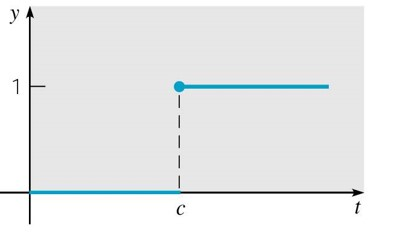
\includegraphics[width=\linewidth]{images/6.3-1.jpg}
\end{image}%
, which you can think of an ``on-switch'' that turns on at \(t=c\). Note that \(1-u_{c}(t)\) is the corresponding ``off-switch'' and looks like: \begin{image}{0.3}{0.4}{0.3}%
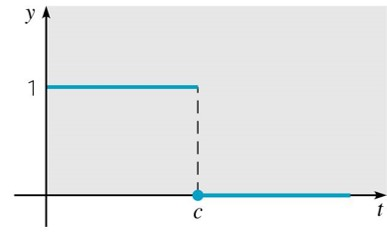
\includegraphics[width=\linewidth]{images/6.3-2.jpg}
\end{image}%
%
\begin{example}{}{g:example:id525051}%
Sketch the following function and describe it as a piecewise function:%
\begin{equation*}
f(t)=2tu_{2}(t)-(t-1)u_{4}(t).
\end{equation*}
%
\par
We look at the critical points which are \(t=2,4\) and consider different cases: \(t\lt2\), \(f(t)=0+0=0\) \(2\leq t\lt4\), \(f(t)=2t\cdot1+0=2t\), \(4\leq t\), \(f(t)=2t\cdot1-(t-1)\cdot1=t+1\), hence%
\begin{equation*}
f(t)=\begin{cases}
0 \amp t\lt 2\\
2t \amp 2\leq t \lt 4\\
t+1 \amp t\geq4.
\end{cases}
\end{equation*}
%
\end{example}
\begin{example}{}{g:example:id525093}%
Write \(f(t)\) in terms of step functions:%
\begin{equation*}
f(t)=\begin{cases}
t \amp 0\leq t\lt 1\\
t-1 \amp 1\leq t\lt 2\\
t-2 \amp 2\leq t\lt 3\\
0 \amp 3\leq t.
\end{cases}
\end{equation*}
%
\par
Solution: The discontinuity points are \(t=0,1,2,3\). When \(0\leq t\lt 1\), the function will be \(f(t)=tu_{0}(t)+\cdots\). Our goal is to figure out the rest. When \(1\leq t\lt 2\), the function will be \(f(t)=tu_{0}(t)+\boldsymbol{?}\cdot u_{1}(t)+\cdots=t-1\), hence%
\begin{equation*}
t+?=t-1\,\,\,\implies?=-1.
\end{equation*}
Hence \(f(t)=tu_{0}(t)-1\cdot u_{1}(t)+\cdots\) When \(2\leq \lt 3\), the function will be \(f(t)=tu_{0}(t)-1\cdot u_{1}(t)+\boldsymbol{?}u_{2}(t)+\cdots=t-2\), hence%
\begin{equation*}
t-1+?=t-2\,\,\,\implies?=-1.
\end{equation*}
Hence \(f(t)=tu_{0}(t)-1\cdot u_{1}(t)-1u_{2}(t)+\cdots\) When \(t\geq3\), the function will be \(f(t)=tu_{0}(t)-1\cdot u_{1}(t)-1u_{2}(t)+\boldsymbol{?}u_{3}(t)\cdots=0\), hence%
\begin{equation*}
t-1-1+?=0\,\,\,\implies?=2-t
\end{equation*}
Thus%
\begin{equation*}
f(t)=tu_{0}(t)-u_{1}(t)-u_{2}(t)+(2-t)u_{3}(t).
\end{equation*}
%
\end{example}
We can compute the Laplace transform of \(u_{c}(t)\):%
\begin{align*}
\mathcal{L}\left\{ u_{c}(t)\right\}  \amp =\int_{0}^{\infty}u_{c}(t)e^{-st}dt=\int_{c}^{\infty}e^{-st}dt\\
\amp =\left[-\frac{e^{-st}}{s}\right]_{t=c}^{t=\infty}\\
\amp =\frac{e^{-cs}}{s}.
\end{align*}
%
\begin{example}{}{g:example:id525150}%
Find the Laplace Transform of%
\begin{equation*}
f(t)=\begin{cases}
2 \amp t\lt3\\
-3 \amp t\geq3
\end{cases}.
\end{equation*}
%
\par
Solution: First use the technique from the first two examples two write \(f(t)\) in terms of \(u_{c}\), and get%
\begin{equation*}
f(t)=2-5u_{3}(t),
\end{equation*}
hence%
\begin{equation*}
F(s)=\mathcal{L}\left\{ f(t)\right\} =\frac{2}{s}-5\frac{e^{-3s}}{s}.
\end{equation*}
%
\end{example}
The theorems that come next are called the \terminology{translation theorems}, because they represent the effect of translation on both functions and their transforms.%
\begin{theorem}{First translation theorem.}{}{g:theorem:id525212}%
If \(F(s)=\mathcal{L}\left\{ f(t)\right\} \) exists for \(s>a\geq0\) and \(c>0\), then%
\begin{equation*}
\mathcal{L}\left\{ u_{c}(t)f\left(t-c\right)\right\} =e^{-cs}\mathcal{L}\left\{ f(t)\right\} =e^{-cs}F(s),
\end{equation*}
Conversely, if \(f(t)=\mathcal{L}^{-1}\left\{ F(s)\right\} \), then%
\begin{equation*}
u_{c}(t)f\left(t-c\right) =\mathcal{L}^{-1}\left\{ e^{-cs}F(s)\right\} .
\end{equation*}
%
\end{theorem}
Remark: Note that \(u_{c}(t)f(t-c)\) translates a function to the right by \(c\), and leaves everything to the left as zero.%
\begin{theorem}{Second translation theorem.}{}{g:theorem:id525254}%
If \(F(s)=\mathcal{L}\left\{ f(t)\right\} \) exists for \(s>a\geq0\) and \(c>0\), then%
\begin{equation*}
\mathcal{L}\left\{ e^{ct}f\left(t\right)\right\} =F(s-c),\,\,\,\,s>a+c.
\end{equation*}
Conversely, if \(f(t)=\mathcal{L}^{-1}\left\{ F(s-c)\right\} \), then%
\begin{equation*}
e^{ct}f(t)=\mathcal{L}^{-1}\left\{ F(s-c)\right\} .
\end{equation*}
%
\end{theorem}
The translation theorems are included in the table formulas:%
\begin{assemblage}{}{g:assemblage:id525279}%
%
\begin{enumerate}
\item{}\(\mathcal{L}\left\{ t^{n}\right\} =\frac{n!}{s^{n+1}}\), \(n\) positive integer.%
\item{}\(\mathcal{L}\left\{ t\right\} =\frac{1}{s^{2}}\), \(\mathcal{L}\left\{ t^{2}\right\} =\frac{2}{s^{3}}\), and \(\mathcal{L}\left\{ t^{3}\right\} =\frac{3!}{s^{4}}\).%
\item{}\(\displaystyle \mathcal{L}\left\{ \sin at\right\} =\frac{a}{s^{2}+a^{2}}\)%
\item{}\(\displaystyle \mathcal{L}\left\{ \cos at\right\} =\frac{s}{s^{2}+a^{2}}\)%
\item{}\(\displaystyle \mathcal{L}\left\{ \sinh at\right\} =\frac{a}{s^{2}-a^{2}}\)%
\item{}\(\displaystyle \mathcal{L}\left\{ \cosh at\right\} =\frac{s}{s^{2}-a^{2}}\)%
\item{}\(\displaystyle \mathcal{L}\left\{ u_{c}(t)f\left(t-c\right)\right\} =e^{-cs}F(s)\)%
\item{}\(\displaystyle \mathcal{L}\left\{ e^{ct}f\left(t\right)\right\} =F(s-c)\)%
\end{enumerate}
%
\end{assemblage}
\begin{example}{}{g:example:id525337}%
Find the Laplace transform of%
\begin{equation*}
f(t)=\begin{cases}
0 \amp t\lt 2\\
t^{2}-4t+5 \amp t\geq2
\end{cases}
\end{equation*}
%
\par
Solution: First we complete the square by adding\slash{}subtracting \(\left(\frac{b}{2}\right)^{2}=\left(\frac{4}{2}\right)^{2}=4\) and get%
\begin{equation*}
t^{2}-4t+5=t^{2}-4t+4-4+5=\left(t-2\right)^{2}-4+5=(t-2)^{2}+1
\end{equation*}
so that%
\begin{align*}
f(t) \amp =\begin{cases}
0 \amp t\lt 2\\
\left(t-2\right)^{2}+1 \amp t\geq2
\end{cases}\\
\amp =u_{2}(t)\left[\left(t-2\right)^{2}+1\right]\\
\amp =u_{2}(t)\left(t-2\right)^{2}+u_{2}(t),
\end{align*}
hence using formulas \(\mathcal{L}\left\{ u_{c}(t)f\left(t-c\right)\right\} =e^{-cs}F(s)\) and \(\mathcal{L}\left\{ t^{2}\right\} =\frac{2}{s^{3}}\) and \(c=2\),%
\begin{align*}
\mathcal{L}\left\{ f(t)\right\}  \amp =e^{-2s}F(s)+\frac{e^{-2s}}{s},\,\,\text{where }f(t-2)=\left(t-2\right)^{2},f(t)=t^{2}\\
\amp =e^{-2s}\frac{2}{s^{3}}+\frac{e^{-2s}}{s}.
\end{align*}
%
\end{example}
\begin{example}{}{g:example:id525343}%
Take the Inverse Laplace Transform of:\({\displaystyle F(s)=\frac{e^{-2s}}{s^{2}+s-2}}\)%
\par
SolutionL In this example we can actually factor%
\begin{align*}
\frac{e^{-2s}}{s^{2}+s-2} \amp =\frac{e^{-2s}}{\left(s+2\right)\left(s-1\right)}\\
\amp =e^{-2s}\left(\frac{-1/3}{s+2}+\frac{1/3}{s-1}\right),\,\text{by partial fractions}
\end{align*}
and use \(\mathcal{L}\left\{ u_{c}(t)f\left(t-c\right)\right\} =e^{-cs}F(s)\) (use this whenever use see an \(e^{-cs}\) when taking \textbackslash{}textbf\textbraceleft{}inverses\textbraceright{}!)%
\begin{align*}
\mathcal{L}^{-1}\left\{ F(s)\right\}  \amp =-\frac{1}{3}\mathcal{L}^{-1}\left\{ \frac{e^{-2s}}{s-(-2)}\right\} +\frac{1}{3}\mathcal{L}^{-1}\left\{ \frac{e^{-2s}}{s-1}\right\} \\
\amp =-\frac{1}{3}u_{2}(t)f_{1}\left(t-2\right)+\frac{1}{3}u_{2}(t)f_{2}\left(t-2\right).
\end{align*}
Use the fact that \(\mathcal{L}\left\{ f_{1}\right\} =\mathcal{L}\left\{ e^{-2t}\right\} =\frac{1}{s+2}\) and \(\mathcal{L}\left\{ f_{2}\right\} =\mathcal{L}\left\{ e^{t}\right\} =\frac{1}{s-1}\) hence%
\begin{equation*}
\mathcal{L}^{-1}\left\{ F(s)\right\} =-\frac{1}{3}u_{2}(t)e^{-2\left(t-2\right)}+\frac{1}{3}u_{2}(t)e^{(t-2)}.
\end{equation*}
%
\end{example}
\begin{example}{}{g:example:id525387}%
Take the Inverse Laplace Transform of:\({\displaystyle F(s)=\frac{9\left(s-3\right)e^{-5s}}{s^{2}-6s+13}}\)%
\par
Solution: In this example we can only complete the square since we can't factor and get%
\begin{equation*}
\frac{9\left(s-3\right)e^{-5s}}{s^{2}-6s+13}=\frac{9\left(s-3\right)e^{-5s}}{\left(s-3\right)^{2}+2^{2}}
\end{equation*}
Now note that by \(\mathcal{L}\left\{ e^{ct}f\left(t\right)\right\} =F(s-c)\) and \(\mathcal{L}\left\{ \cos at\right\} =\frac{s}{s^{2}+a^{2}}\) we have%
\begin{align*}
\mathcal{L}\left\{ \cos\left(2t\right)\right\} =\frac{s}{s^{2}+2^{2}} \amp \implies\mathcal{L}\left\{ e^{3t}\cos\left(2t\right)\right\} =\frac{(s-3)}{(s-3)^{2}+2^{2}}
\end{align*}
(Need to take care of the \(e^{-5s}\)) Now use \(\mathcal{L}\left\{ u_{c}(t)f_{1}\left(t-c\right)\right\} =e^{-cs}F_{1}(s)\) with \(f_{1}(t)=e^{3t}\cos\left(2t\right)\) and \(c=5\) so that \(f_{1}(t-5)=e^{3(t-5)}\cos\left(2\left(t-5\right)\right)\) hence%
\begin{equation*}
\mathcal{L}\left\{ u_{5}(t)e^{3(t-5)}\cos\left(2\left(t-5\right)\right)\right\} =e^{-5s}\frac{(s-3)}{(s-3)^{2}+2^{2}}
\end{equation*}
Thus multiplying both sides by \(9\)%
\begin{equation*}
\mathcal{L}^{-1}\left\{ F(s)\right\} =9u_{5}(t)e^{3(t-5)}\cos\left(2\left(t-5\right)\right).
\end{equation*}
%
\end{example}
\begin{example}{}{g:example:id525458}%
Take the Inverse Laplace Transform of:\({\displaystyle F(s)=\frac{e^{-7s}}{s^{2}-4}}\).%
\par
Solution: We note \(\mathcal{L}\left\{ \sinh2t\right\} =\frac{2}{s^{2}-4}\) and use \(\mathcal{L}\left\{ u_{c}(t)f_{1}\left(t-c\right)\right\} =e^{-cs}F_{1}(s)\) where \(f_{1}(t)=\sinh2t\implies f_{1}(t-7)=\sinh2\left(t-7\right)\) to get that%
\begin{align*}
\mathcal{L}\left\{ u_{7}(t)f_{1}\left(t-7\right)\right\} =e^{-7s}F_{1}(s), \amp \implies\mathcal{L}\left\{ u_{7}(t)\sinh2\left(t-7\right)\right\} =\frac{2e^{-7s}}{s^{2}-4}\\
\amp \implies\frac{1}{2}\mathcal{L}\left\{ u_{7}(t)\sinh2\left(t-7\right)\right\} =\frac{e^{-7s}}{s^{2}-4}
\end{align*}
hence%
\begin{equation*}
\mathcal{L}^{-1}\left\{ F(s)\right\} =\frac{1}{2}u_{7}(t)\sinh2\left(t-7\right).
\end{equation*}
%
\end{example}
\begin{example}{}{g:example:id525473}%
Take the Inverse Laplace Transform of:\({\displaystyle F(s)=\frac{1}{s^{2}}+\frac{e^{-6s}}{\left(s-2\right)^{3}}}\).%
\par
We know \(\mathcal{L}\left\{ t\right\} =\frac{1}{s^{2}}\), \(\mathcal{L}\left\{ t^{2}\right\} =\frac{2}{s^{3}}\) and \(\mathcal{L}\left\{ e^{ct}f\left(t\right)\right\} =F(s-c)\) and \(\mathcal{L}\left\{ u_{c}(t)f\left(t-c\right)\right\} =e^{-cs}F(s)\) hence%
\begin{align*}
\mathcal{L}^{-1}\left\{ F(s)\right\}  \amp =t+\frac{1}{2}\mathcal{L}^{-1}\left\{ \frac{2e^{-6s}}{\left(s-2\right)^{3}}\right\} \\
\amp =t+\frac{1}{2}u_{6}(t)e^{2(t-6)}(t-6)^{2}.
\end{align*}
%
\end{example}
\begin{example}{}{g:example:id525513}%
Take the Inverse Laplace Transform of: \({\displaystyle F(s)=\frac{1}{s^{2}-10s+26}}\).%
\par
Solution: (practice with using \(\mathcal{L}\left\{ e^{ct}g\left(t\right)\right\} =G(s-c)\)). First we complete the square and get%
\begin{equation*}
\frac{1}{s^{2}-10s+26}=\frac{1}{\left(s-5\right)^{2}+1}
\end{equation*}
and use \(\mathcal{L}\left\{ \sin at\right\} =\frac{a}{s^{2}+a^{2}}\) with \(a=1\) so that \(\mathcal{L}\left\{ \sin t\right\} =\frac{1}{s^{2}+1}\) Then use the fact that \(\mathcal{L}\left\{ e^{ct}g\left(t\right)\right\} =G(s-c)\) with \(c=5\) and \(g(t)=\sin t\), thus we know that%
\begin{equation*}
\mathcal{L}\left\{ e^{5t}\sin t\right\} =\frac{1}{\left(s-5\right)^{2}+1}
\end{equation*}
hence%
\begin{equation*}
\mathcal{L}^{-1}\left\{ F(s)\right\} =e^{5t}\sin t.
\end{equation*}
%
\end{example}
\end{sectionptx}
%
%
\typeout{************************************************}
\typeout{Section 6.5 ODEs with discontinuous forcing functions}
\typeout{************************************************}
%
\begin{sectionptx}{ODEs with discontinuous forcing functions}{}{ODEs with discontinuous forcing functions}{}{}{x:section:ch6-5}
We will now do some examples involving intial value problems where the forcing function have pieces that switch on and off. This will require the use of step functions to turn parts of the forcing function on and off as the definition requires. You can think of this as a way to rewrite a multi-part definition into just one definition for a piecewise continuous function.%
\begin{example}{}{g:example:id525577}%
Solve using Laplace Transforms:%
\begin{equation*}
y^{\prime}=-y+u_{3}(t),\,\,\,\,\,y(0)=2.
\end{equation*}
%
\par
Step 1: Take \(\mathcal{L}\) of both sides and solve for \(\mathcal{L}\)%
\begin{equation*}
\mathcal{L}\left\{ y^{\prime}\right\} =\mathcal{L}\left\{ -y\right\} +\mathcal{L}\left\{ u_{3}(t)\right\} 
\end{equation*}
so that%
\begin{equation*}
s\mathcal{L}\left\{ y\right\} -y(0)=-\mathcal{L}\left\{ y\right\} +\frac{e^{-3s}}{s}.
\end{equation*}
%
\par
Step 2: Solve for \(\mathcal{L}\left\{ y\right\} \),%
\begin{equation*}
\mathcal{L}\left\{ y\right\} =\frac{2}{s+1}+\frac{e^{-3s}}{s\left(s+1\right)}
\end{equation*}
%
\par
Step 3: We do partial fractions on%
\begin{equation*}
\frac{1}{s\left(s+1\right)}=\frac{1}{s}-\frac{1}{s+1}
\end{equation*}
%
\par
Step 4: Take the inverse Laplace transform: Using \(\mathcal{L}\left[u_{a}(t)f(t-a)\right]=e^{-as}F(s)\), and get%
\begin{align*}
y \amp =\mathcal{L}^{-1}\left\{ \frac{2}{s+1}+e^{-3s}\frac{1}{s}-e^{-3s}\frac{1}{s+1}\right\} \\
\amp =2e^{-t}+u_{3}(t)-u_{3}(t)e^{-\left(t-3\right)}.
\end{align*}
%
\end{example}
\begin{example}{}{g:example:id525644}%
Solve using Laplace Transforms:%
\begin{equation*}
y^{\prime}=-3y+6u_{4}(t)e^{-\left(t-4\right)},\,\,\,\,\,y(0)=5.
\end{equation*}
%
\par
Step 1: Take \(\mathcal{L}\) of both sides%
\begin{equation*}
\mathcal{L}\left\{ y^{\prime}\right\} =-3\mathcal{L}\left\{ y\right\} +6\mathcal{L}\left\{ u_{4}(t)e^{-\left(t-4\right)}\right\} 
\end{equation*}
and get%
\begin{equation*}
s\mathcal{L}\left\{ y\right\} -y(0)=-3\mathcal{L}\left\{ y\right\} +6\mathcal{L}\left\{ u_{4}(t)e^{-\left(t-4\right)}\right\} 
\end{equation*}
%
\par
Step 2: Solve for \(\mathcal{L}\left\{ y\right\} \) and get%
\begin{equation*}
\mathcal{L}\left\{ y\right\} =\frac{5}{s+3}+\frac{6e^{-4s}}{\left(s+3\right)\left(s+1\right)}.
\end{equation*}
%
\par
Step 3: We do partial fractions%
\begin{equation*}
\frac{6}{\left(s+3\right)\left(s+1\right)}=\frac{-3}{\left(s+3\right)}+\frac{3}{\left(s+1\right)}.
\end{equation*}
%
\par
Step 3: Take the inverse Laplace transform: Using \(\mathcal{L}\left[u_{a}(t)f(t-a)\right]=e^{-as}F(s)\), and%
\begin{align*}
y \amp =\mathcal{L}^{-1}\left\{ \frac{5}{s+3}+\frac{6e^{-4s}}{\left(s+3\right)\left(s+1\right)}\right\} \\
\amp =\mathcal{L}^{-1}\left\{ \frac{5}{s+3}\right\} +\mathcal{L}^{-1}\left\{ -3e^{-4s}\frac{1}{\left(s+3\right)}+3e^{-4s}\frac{1}{\left(s+1\right)}\right\} \\
\amp =5e^{-3t}-3u_{4}(t)e^{-3\left(t-4\right)}+3u_{4}(t)e^{-\left(t-4\right)}.
\end{align*}
%
\end{example}
\begin{example}{}{g:example:id525650}%
Solve using Laplace Transforms:%
\begin{equation*}
y^{\prime\prime}+4y=3u_{5}(t)\sin\left(t-5\right),\,\,\,\,\,y(0)=1,y^{\prime}(0)=0.
\end{equation*}
%
\par
Step 1: Take \(\mathcal{L}\) of both sides and solve for \(\mathcal{L}\)%
\begin{equation*}
\mathcal{L}\left\{ y^{\prime\prime}\right\} +4\mathcal{L}\left\{ y\right\} =3\mathcal{L}\left\{ u_{5}(t)\sin\left(t-5\right)\right\} 
\end{equation*}
and recall \(\mathcal{L}\left[u_{a}(t)f(t-a)\right]=e^{-as}F(s)\), hence \(a=4\), \(f(t-5)=\sin\left(t-5\right)\) hence \(f(t)=\sin t\) and \(\mathcal{L}\left\{ \sin t\right\} =\frac{1}{s^{2}+1}\) hence%
\begin{align*}
s^{2}\mathcal{L}\left\{ y\right\} -sy(0)-y^{\prime}(0)+4\mathcal{L}\left\{ y\right\}  \amp =3\frac{e^{-5s}}{s^{2}+1},\implies\\
\left(s^{2}+4\right)\mathcal{L}\left\{ y\right\} -s \amp =3\frac{e^{-5s}}{s^{2}+1},\implies\\
\mathcal{L}\left\{ y\right\}  \amp =3\frac{e^{-5s}}{\left(s^{2}+4\right)\left(s^{2}+1\right)}+\frac{s}{s^{2}+4}
\end{align*}
%
\par
Step 2: We do partial fractions on%
\begin{equation*}
\frac{3}{\left(s^{2}+4\right)\left(s^{2}+1\right)}=\frac{As+B}{s^{2}+4}+\frac{Cs+D}{s^{2}+1}
\end{equation*}
hence%
\begin{align*}
3 \amp =\left(As+B\right)\left(s^{2}+1\right)+\left(Cs+D\right)\left(s^{2}+4\right),\implies\\
0\cdot s^{3}+0\cdot s^{2}+0\cdot s+3 \amp =\left(A+C\right)s^{3}+\left(B+D\right)s^{2}+\left(A+4C\right)s+\left(B+4D\right)
\end{align*}
hence%
\begin{align*}
A+C \amp =0\\
B+D \amp =0\\
A+4C \amp =0\\
B+4D \amp =3
\end{align*}
and get%
\begin{equation*}
A=0\,\,\,\,B=-1,\,\,\,\,C=0,\,\,\,D=1
\end{equation*}
hence%
\begin{equation*}
\frac{3}{\left(s^{2}+4\right)\left(s^{2}+1\right)}=\frac{-1}{s^{2}+4}+\frac{1}{s^{2}+1}
\end{equation*}
%
\par
Step 3: Take the inverse Laplace transform: Using \(\mathcal{L}\left[u_{a}(t)f(t-a)\right]=e^{-as}F(s)\), and \(\mathcal{L}\left\{ \sin(at)\right\} =\frac{a}{s^{2}+a^{2}}\) and \(\mathcal{L}\left\{ \cos(at)\right\} =\frac{a}{s^{2}+a^{2}}\) we have%
\begin{align*}
y \amp =\mathcal{L}^{-1}\left\{ \frac{-e^{-5s}}{s^{2}+4}+\frac{e^{-5s}}{s^{2}+1}+\frac{s}{s^{2}+4}\right\} \\
\amp =-\frac{1}{2}\mathcal{L}^{-1}\left\{ \frac{2e^{-5s}}{s^{2}+2^{2}}\right\} +\mathcal{L}^{-1}\left\{ \frac{e^{-5s}}{s^{2}+1}\right\} +\mathcal{L}^{-1}\left\{ \frac{s}{s^{2}+4}\right\} \\
\amp =-\frac{1}{2}u_{5}(t)\sin\left(2\left(t-5\right)\right)+u_{5}(t)\sin\left(t-5\right)+\cos\left(2t\right)
\end{align*}
%
\end{example}
\begin{example}{}{g:example:id525763}%
Solve using Laplace Transforms:%
\begin{equation*}
y^{(4)}-y=u_{1}(t)-u_{2}(t),\,\,\,\,\,y(0)=0,y^{\prime}(0)=0,y^{\prime\prime}(0)=0.,y^{\prime\prime\prime}(0)=0..
\end{equation*}
%
\par
Step 1: Take \(\mathcal{L}\) of both sides and solve for \(\mathcal{L}\)%
\begin{equation*}
\mathcal{L}\left\{ y^{(4)}\right\} -\mathcal{L}\left\{ y\right\} =\mathcal{L}\left\{ u_{1}(t)-u_{2}(t)\right\} 
\end{equation*}
hence%
\begin{align*}
\amp s^{4}\mathcal{L}\left\{ y\right\} -s^{3}y(0)-s^{2}y^{\prime}(0)-sy^{\prime\prime}(0)-sy^{\prime\prime\prime}-y^{\prime}(0)-\mathcal{L}\left\{ y\right\}\\
\amp =\frac{e^{-s}}{s}-\frac{e^{-2s}}{s}\implies\\
\left(s^{4}-1\right)\mathcal{L}\left\{ y\right\}  \amp =\frac{e^{-s}}{s}-\frac{e^{-2s}}{s},\implies\\
\mathcal{L}\left\{ y\right\}  \amp =\frac{e^{-s}}{s\left(s^{4}-1\right)}-\frac{e^{-2s}}{s\left(s^{4}-1\right)}
\end{align*}
%
\par
Step 2: We do partial fractions on%
\begin{equation*}
\frac{1}{s\left(s^{4}-1\right)}=\frac{1}{s\left(s^{2}-1\right)\left(s^{2}+1\right)}=\frac{1}{s\left(s+1\right)\left(s-1\right)\left(s^{2}+1\right)}=
\end{equation*}
hence%
\begin{equation*}
\frac{1}{s\left(s^{4}-1\right)}=\frac{A}{s}+\frac{B}{s+1}+\frac{C}{s-1}+\frac{Ds+E}{s^{2}+1}
\end{equation*}
after doing the work to get the partial fractions you get%
\begin{equation*}
\frac{1}{s\left(s^{4}-1\right)}=-\frac{1}{s}+\frac{1}{4}\frac{1}{s+1}+\frac{1}{4}\frac{1}{s-1}+\frac{1}{2}\frac{s}{s^{2}+1}
\end{equation*}
putting it back we need to take the inverse of%
\begin{align*}
\amp e^{-s}\left[-\frac{1}{s}+\frac{1}{4}\frac{1}{s+1}+\frac{1}{4}\frac{1}{s-1}+\frac{1}{2}\frac{s}{s^{2}+1}\right]\\
\amp -e^{-2s}\left[-\frac{1}{s}+\frac{1}{4}\frac{1}{s+1}+\frac{1}{4}\frac{1}{s-1}+\frac{1}{2}\frac{s}{s^{2}+1}\right]
\end{align*}
%
\par
Step 3: Take the inverse Laplace transform: Using \(\mathcal{L}\left[u_{a}(t)f(t-a)\right]=e^{-as}F(s)\), and \(\mathcal{L}\left\{ \cos(at)\right\} =\frac{a}{s^{2}+a^{2}}\) and \(\mathcal{L}\left\{ e^{at}\right\} =\frac{1}{s-a}\) we have%
\begin{align*}
y \amp =\mathcal{L}^{-1}\left\{ e^{-s}\left[-\frac{1}{s}+\frac{1}{4}\frac{1}{s+1}+\frac{1}{4}\frac{1}{s-1}+\frac{1}{2}\frac{s}{s^{2}+1}\right]\right\} \\
\amp -\mathcal{L}^{-1}\left\{ e^{-2s}\left[-\frac{1}{s}+\frac{1}{4}\frac{1}{s+1}+\frac{1}{4}\frac{1}{s-1}+\frac{1}{2}\frac{s}{s^{2}+1}\right]\right\} \\
\amp =-u_{1}(t)+u_{1}(t)\left[\frac{1}{4}e^{-1\left(t-1\right)}+\frac{1}{4}e^{1\left(t-1\right)}+\frac{1}{2}\cos\left(t-1\right)\right]\\
\amp +u_{2}(t)-u_{2}(t)\left\{ \frac{1}{4}e^{-1\left(t-2\right)}+\frac{1}{4}e^{1\left(t-2\right)}+\frac{1}{2}\cos\left(t-2\right)\right\} 
\end{align*}
%
\end{example}
\begin{example}{}{g:example:id525859}%
Find the Laplace transform of%
\begin{equation*}
f(t)=\begin{cases}
t \amp 0\leq t\lt 1\\
3t \amp 1\leq t\lt\infty
\end{cases}.
\end{equation*}
%
\par
Step 1: First let us rewrite this in terms of unit step functions. When \(0\leq t\lt 1\): the function is \(f(t)=t\) When \(1\leq t\lt \infty\): then function is \(f(t)=t+?\cdot u_{1}(t)=3t\) hence \(?=2t\) so that%
\begin{equation*}
f(t)=t+2tu_{1}(t).
\end{equation*}
%
\par
Step 2: Before we can take a Laplace transform, we notice that our fomula involves \(\mathcal{L}\left\{ u_{c}(t)g\left(t-c\right)\right\} =e^{-ct}\mathcal{L}\left\{ g(t)\right\} \). Thus we will need to turn \(2tu_{1}(t)\) into this form:%
\begin{align*}
f(t) \amp =t+2tu_{1}(t)\\
\amp =t+2\left(t-\boldsymbol{1}\right)u_{1}(t)+\boldsymbol{2u_{1}(t)}
\end{align*}
hence%
\begin{align*}
\mathcal{L}\left\{ f(t)\right\}  \amp =\mathcal{L}\left\{ t\right\} +2\mathcal{L}\left\{ (t-1)u_{1}(t)\right\} +2\mathcal{L}\left\{ u_{1}(t)\right\} \\
\amp =\frac{1}{s^{2}}+2e^{-s}\frac{1}{s^{2}}+2e^{-s}\frac{1}{s}.
\end{align*}
%
\end{example}
We now introduce the following useful formula that is not included in the table, which records the translation of a step function:%
\begin{fact}{}{}{g:fact:id525890}%
We have%
\begin{equation*}
\mathcal{L}\left\{ u_{c}(t)h(t)\right\} =e^{-cs}\mathcal{L}\left\{ h\left(t+c\right)\right\} .
\end{equation*}
%
\end{fact}
\begin{example}{}{g:example:id525896}%
Take the Laplace transform of \(f(t)=u_{1}(t)te^{t}\).%
\par
Notice that we cannot use the formula \(\mathcal{L}\left\{ u_{c}(t)g\left(t-c\right)\right\} =e^{-ct}\mathcal{L}\left\{ g(t)\right\} \) directly since \(te^{t}\) is not written as a function of \((t-1)\). Hence we'll need to use \(\mathcal{L}\left\{ u_{c}(t)h(t)\right\} =e^{-cs}\mathcal{L}\left\{ h\left(t+c\right)\right\} \) with \(h(t)=te^{t}\) and \(c=1\). Thus%
\begin{equation*}
h\left(t+1\right)=(t+1)e^{t+1}
\end{equation*}
and we get%
\begin{align*}
\mathcal{L}\left\{ u_{1}(t)te^{t}\right\}  \amp =e^{-cs}\mathcal{L}\left\{ h\left(t+c\right)\right\} \\
\amp =e^{-s}\mathcal{L}\left\{ (t+1)e^{t+1}\right\} \\
\amp =e^{-s}\mathcal{L}\left\{ te^{t}e+e^{t}e\right\} \\
\amp =e^{-s}\left(e\mathcal{L}\left\{ te^{t}\right\} +e\mathcal{L}\left\{ e^{t}\right\} \right)\\
\amp =e^{1-s}\left(\frac{1}{\left(s-1\right)^{2}}+\frac{1}{\left(s-1\right)}\right)
\end{align*}
where we used formula \(2\) and \(11\) in the table.%
\end{example}
\end{sectionptx}
%
%
\typeout{************************************************}
\typeout{Section 6.6 Impulse functions}
\typeout{************************************************}
%
\begin{sectionptx}{Impulse functions}{}{Impulse functions}{}{}{x:section:ch6-6}
One of the most useful capabilities of the Laplace transform is to deal with forcing functions that aren't even functions, but that occur with great regularity in the modeling of physical systems. The guiding question here that we should keep in mind is ``what happens to an oscillating mass when it gets struck by an outside blow?''.%
\par
We consider%
\begin{equation*}
ay^{\prime\prime}+by^{\prime}+cy=f(t),
\end{equation*}
where%
\begin{align*}
g(t) \amp =\begin{cases}
\text{large } \amp t_{0}-\tau\lt t\lt t_{0}+\tau.\\
0 \amp \text{elsewhere}
\end{cases}
\end{align*}
Here \(g(t)\) is a \terminology{force} and%
\begin{equation*}
I(\tau)=\int_{t_{0}-\tau}^{t_{0}+\tau}g(t)dt=\int_{-\infty}^{\infty}g(t)dt
\end{equation*}
is the \terminology{impulse} of the force, or the amount of force in a short time period about \(t_{0}\).%
\par
If \(y=\)current in an electric circuit, \(g(t)=\) is the time derivative of the voltage, then \(I(\tau)\) is the total voltage impressed on circuit in the time interval \(I=\left(t_{0}-\tau,t_{0}+\tau\right)\). We will use the following particular example of a force with \(\tau=0\) (to simplify things):%
\begin{equation*}
g(t)=d_{\tau}(t)=\begin{cases}
\frac{1}{2\tau} \amp -\tau\lt t\lt \tau,\\
0 \amp \text{elsewhere}
\end{cases},
\end{equation*}
where \(\tau>0\) is small.%
\par
We'll first look at some nice properties of \(d_{\tau}(t)\):%
\begin{enumerate}
\item{}\({\displaystyle \lim_{\tau\to0^{+}}d_{\tau}(t)=0}\), whenever \(t\neq0\), and \(\lim_{\tau\to0^{+}}d_{\tau}(0)=\infty\). \begin{image}{0}{1}{0}%
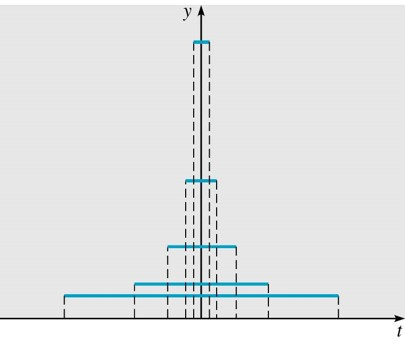
\includegraphics[width=\linewidth]{images/6.5-1.jpg}
\end{image}%
%
\item{}\(I(\tau)=\int_{-\tau}^{\tau}\frac{1}{2\tau}dt=\left[\frac{1}{2\tau}t\right]_{-\tau}^{\tau}=1\) for every \(\tau\). Hence \({\displaystyle \lim_{\tau\to0^{+}}}I(\tau)=1\), \begin{image}{0}{1}{0}%
\includegraphics[width=\linewidth]{images/6.5-2.jpg}
\end{image}%
%
\end{enumerate}
%
\par
We thus want to define a \terminology{unit impulse function \(\delta\)}, with the properties%
\begin{equation*}
\delta(t)=\begin{cases}
0 \amp t\neq0\\
\infty \amp t=0
\end{cases}
\end{equation*}
and%
\begin{equation*}
\int_{-\infty}^{\infty}\delta(t)dt=1.
\end{equation*}
%
\par
This object isn't actually a function, but there is a mathematically rigorous way to define objects called \emph{generalized functions} which includes \(\delta\). We call \(\delta\) the \terminology{Dirac delta function}. We can think of \(\delta\) as a limit of the \(d_{\tau}(t)\) functions:%
\begin{equation*}
\delta(t)=\lim_{\tau\to0^{+}}d_{\tau}(t).
\end{equation*}
%
\par
We can consider a unit impulse at an arbitrary point \(t=t_{0}\), meaning \(\delta\left(t-t_{0}\right)\), hence%
\begin{align*}
\delta\left(t-t_{0}\right) \amp =0,\,\,t\neq t_{0},\\
\int_{-\infty}^{\infty}\delta(t-t_{0})dt \amp =1.
\end{align*}
We will now compute the Laplace Transform of \(\delta\left(t-t_{0}\right)\), using the properties of the integral definition:%
\begin{align*}
\mathcal{L}\left\{ \delta\left(t-t_{0}\right)\right\}  \amp =\lim_{\tau\to0^{+}}\mathcal{L}\left\{ d_{\tau}\left(t-t_{0}\right)\right\} \\
\amp =\lim_{\tau\to0^{+}}\int_{t_{0}-\tau}^{t_{0}+\tau}e^{-st}d_{\tau}\left(t-t_{0}\right)dt\\
\amp =\lim_{\tau\to0^{+}}\frac{1}{2\tau}\int_{t_{0}-\tau}^{t_{0}+\tau}e^{-st}dt=\lim_{\tau\to0^{+}}\frac{1}{2\tau}\left[\frac{e^{-st}}{t}\right]_{t=t_{0}-\tau}^{t=t_{0}+\tau}\\
\amp =\frac{e^{-st_{0}}}{s}\lim_{\tau\to0^{+}}\frac{e^{s\tau}-e^{-s\tau}}{2\tau},\text{ by algebra}\\
\amp =e^{-st_{0}}\lim_{\tau\to0^{+}}\frac{\sinh(s\tau)}{s\tau},\text{ by formula below}\\
\amp =e^{-st_{0}}\lim_{\tau\to0^{+}}\frac{s\cosh(s\tau)}{s},\text{ by L'Hopitals rule}\\
\amp =e^{-st_{0}}.
\end{align*}
where we used the fact that%
\begin{equation*}
\sinh(s\tau)=\frac{e^{s\tau}-s^{-s\tau}}{2}.
\end{equation*}
In summary,%
\begin{equation*}
\mathcal{L}\left\{ \delta\left(t-t_{0}\right)\right\} =e^{-st_{0}},\,\,\,t_{0}>0.
\end{equation*}
%
\par
We now compute some simple examples:%
%
\begin{itemize}[label=\textbullet]
\item{}If \(t_{0}=0\), then%
\begin{equation*}
\mathcal{L}\left\{ \delta\left(t\right)\right\} =e^{-s\cdot0}=1.
\end{equation*}
%
\item{}If \(t_{0}=9\) then%
\begin{equation*}
\mathcal{L}\left\{ \delta\left(t-9\right)\right\} =e^{-9s}.
\end{equation*}
%
\end{itemize}
We'll note the following important property of \(\delta\) functions, which is usually called ``point evaluation''. Suppose \(f\) is a continuous function. Then%
\begin{equation*}
\int_{-\infty}^{\infty}f(t)\delta(t-t_{0})dt=f\left(t_{0}\right).
\end{equation*}
%
\par
In the next example we show how the delta function is connected to the Heaviside function.%
\begin{example}{}{g:example:id526197}%
Solve the IVP%
\begin{equation*}
y^{\prime}=\delta(t-c),\,\,\,\,y(0)=y_{0}.
\end{equation*}
%
\par
Take \(\mathcal{L}\) of both sides and%
\begin{align*}
\mathcal{L}\left\{ y^{\prime}\right\} =\mathcal{L}\left\{ \delta\left(t-c\right)\right\}  \amp \implies\\
s\mathcal{L}\left\{ y\right\} -y(0)=e^{-cs} \amp \implies\\
\mathcal{L}\left\{ y\right\} =\frac{y_{0}}{s}+\frac{e^{-cs}}{s}
\end{align*}
hence%
\begin{align*}
y \amp =\mathcal{L}^{-1}\left\{ \frac{y_{0}}{s}\right\} +\mathcal{L}^{-1}\left\{ \frac{e^{-cs}}{s}\right\} \\
\amp =y_{0}+u_{c}(t).
\end{align*}
%
\end{example}
The example shows that the derivative of the Heaviside function is the delta function! (To be totally clear, we should note that to define derivatives of discontinuous functions requires that we understand differentiation in the context of generalized functions. For now, we should accept the intuition that the ``slope'' of a jump dicontinuity is the ``infinite spike'' of the delta function.%
\begin{fact}{}{}{g:fact:id526221}%
%
\begin{equation*}
\frac{d}{dt}\left[u_{c}(t)\right]=\delta\left(t-c\right).
\end{equation*}
\end{fact}
\begin{example}{}{g:example:id526256}%
Solve the IVP%
\begin{equation*}
y^{\prime\prime}+4y=\delta\left(t-\pi\right)-\delta\left(t-2\pi\right),\,\,\,\,y(0)=0,y^{\prime}(0)=0.
\end{equation*}
%
\par
Step 1: Take \(\mathcal{L}\) of both sides and solve for \(\mathcal{L}\left\{ y\right\} \):%
\begin{align*}
\mathcal{L}\left\{ y^{\prime\prime}\right\} +4\mathcal{L}\left\{ y\right\} =\mathcal{L}\left\{ \delta\left(t-\pi\right)\right\} -\mathcal{L}\left\{ \delta\left(t-2\pi\right)\right\}  \amp \implies\\
s^{2}\mathcal{L}\left\{ y\right\} -sy(0)-y^{\prime}(0)+4\mathcal{L}\left\{ y\right\} =e^{-\pi s}-e^{-2\pi s} \amp \implies\\
\left(s^{2}+4\right)\mathcal{L}\left\{ y\right\} =e^{-\pi s}-e^{-2\pi s} \amp \implies\\
\mathcal{L}\left\{ y\right\} =\frac{e^{-\pi s}}{s^{2}+4}-\frac{e^{-2\pi s}}{s^{2}+4}.
\end{align*}
%
\par
Step 2: Notice that we don't need to do partial fractions or complete the square here since \(s^{2}+4\) is already a sum of two squares.%
\par
Step3: Take an inverse Laplace transform: Using \(\mathcal{L}\left[u_{a}(t)f(t-a)\right]=e^{-as}F(s)\) and \(\mathcal{L}\left\{ \sin(at)\right\} =\frac{a}{s^{2}+a^{2}}\) we get%
\begin{align*}
y \amp =\mathcal{L}^{-1}\left\{ \frac{e^{-\pi s}}{s^{2}+4}\right\} -\mathcal{L}^{-1}\left\{ \frac{e^{-2\pi s}}{s^{2}+4}\right\} \\
\amp =\frac{1}{2}\mathcal{L}^{-1}\left\{ e^{-\pi s}\frac{2}{s^{2}+2^{2}}\right\} -\frac{1}{2}\mathcal{L}^{-1}\left\{ e^{-2\pi s}\frac{2}{s^{2}+2^{2}}\right\} \\
\amp =\frac{1}{2}u_{\pi}(t)f_{1}\left(t-\pi\right)-\frac{1}{2}u_{2\pi}(t)f_{2}\left(t-2\pi\right)\\
\amp =\frac{1}{2}u_{\pi}(t)\sin\left(2\left(t-\pi\right)\right)-\frac{1}{2}u_{2\pi}(t)\sin\left(2\left(t-2\pi\right)\right)
\end{align*}
where \(f_{1},f_{2}=\sin(2t)\). Now it turns out, that%
\begin{equation*}
\sin\left(2\left(t-\pi\right)\right)=\sin\left(2t-2\pi\right)=\sin(2t)
\end{equation*}
and%
\begin{equation*}
\sin\left(2\left(t-2\pi\right)\right)=\sin\left(2t-4\pi\right)=\sin(2t).
\end{equation*}
or in general%
\begin{equation*}
\sin\left(x\right)=\sin\left(x+2\pi\right).
\end{equation*}
Hence a possible multiple choice answer could be:%
\begin{equation*}
y=\frac{1}{2}u_{\pi}(t)\sin\left(2t\right)-\frac{1}{2}u_{2\pi}(t)\sin\left(2t\right).
\end{equation*}
%
\end{example}
\begin{example}{}{g:example:id526326}%
Solve the IVP%
\begin{equation*}
y^{\prime\prime}+2y^{\prime}+3y=\sin t+\delta\left(t-3\pi\right),\,\,\,\,y(0)=0,y^{\prime}(0)=0.
\end{equation*}
%
\par
Take \(\mathcal{L}\) of both sides and solve for \(\mathcal{L}\left\{ y\right\} \):%
\begin{align*}
\mathcal{L}\left\{ y^{\prime\prime}\right\} +2\mathcal{L}\left\{ y^{\prime}\right\} +3\mathcal{L}\left\{ y\right\} =\frac{1}{s^{2}+1}+e^{-3\pi s} \amp \implies\\
\left[s^{2}\mathcal{L}\left\{ y\right\} -sy(0)-y^{\prime}(0)\right]+2\left[s\mathcal{L}\left\{ y\right\} -y(0)\right]+3\mathcal{L}\left\{ y\right\} =\frac{1}{s^{2}+1}+e^{-3\pi s} \amp \implies\\
s^{2}\mathcal{L}\left\{ y\right\} +2s\mathcal{L}\left\{ y\right\} +3\mathcal{L}\left\{ y\right\} =\frac{1}{s^{2}+1}+e^{-3\pi s} \amp \implies\\
\left(s^{2}+2s+3\right)\mathcal{L}\left\{ y\right\} =\frac{1}{s^{2}+1}+e^{-3\pi s} \amp \implies\\
\mathcal{L}\left\{ y\right\} =\frac{1}{\left(s^{2}+2s+3\right)\left(s^{2}+1\right)}+\frac{e^{-3\pi s}}{s^{2}+2s+3}
\end{align*}
%
\par
Step 2: First we do partial fractions:%
\begin{equation*}
\frac{1}{\left(s^{2}+2s+3\right)\left(s^{2}+1\right)}=\frac{As+B}{\left(s^{2}+2s+3\right)}+\frac{Cs+D}{\left(s^{2}+1\right)}
\end{equation*}
and do the algebra to get%
\begin{equation*}
A=\frac{1}{4},B=\frac{1}{4},C=-\frac{1}{4},D=\frac{1}{4}
\end{equation*}
Also we need to complete the square:%
\begin{equation*}
s^{2}+2s+3=\left(s+1\right)^{2}+2.
\end{equation*}
so that%
\begin{equation*}
\frac{1}{\left(s^{2}+2s+3\right)\left(s^{2}+1\right)}=\frac{1}{4}\left(\frac{s+1}{\left(s+1\right)^{2}+2}+\frac{-s+1}{\left(s^{2}+1\right)}\right)
\end{equation*}
%
\par
Step 3: Take an inverse Laplace transform: Using \(\mathcal{L}\left[u_{a}(t)f(t-a)\right]=e^{-as}F(s)\) , \(\mathcal{L}\left\{ \cos(at)\right\} =\frac{s}{s^{2}+a^{2}}\) \(\mathcal{L}\left\{ \sin(at)\right\} =\frac{a}{s^{2}+a^{2}}\) , Also using \(\mathcal{L}\left\{ e^{at}\cos(bt)\right\} =\frac{s-a}{(s-a)^{2}+b^{2}}\) \(\mathcal{L}\left\{ e^{at}\sin(bt)\right\} =\frac{b}{(s-a)^{2}+b^{2}}\) we get%
\begin{align*}
y \amp =\frac{1}{4}\mathcal{L}^{-1}\left\{ \frac{s+1}{\left(s+1\right)^{2}+2}\right\} +\frac{1}{4}\mathcal{L}^{-1}\left\{ \frac{-s+1}{\left(s^{2}+1\right)}\right\} \\
\amp +\mathcal{L}^{-1}\left\{ \frac{e^{-3\pi s}}{\left(s+1\right)^{2}+2}\right\} \\
\amp =\frac{1}{4}\mathcal{L}^{-1}\left\{ \frac{s+1}{\left(s+1\right)^{2}+\left(\sqrt{2}\right)^{2}}\right\} -\frac{1}{4}\mathcal{L}^{-1}\left\{ \frac{s}{s^{2}+1}\right\} \\
\amp +\frac{1}{4}\mathcal{L}^{-1}\left\{ \frac{1}{s^{2}+1}\right\} +\frac{1}{\sqrt{2}}\mathcal{L}^{-1}\left\{ e^{-3\pi s}\frac{\sqrt{2}}{\left(s+1\right)^{2}+\left(\sqrt{2}\right)^{2}}\right\} \\
\amp =\frac{1}{4}\left(e^{-t}\cos\left(\sqrt{2}t\right)-\cos t+\sin t\right)\\
\amp +\frac{1}{\sqrt{2}}u_{3\pi}\left(t\right)f_{1}\left(t-3\pi\right)\\
\amp =\frac{1}{4}\left(e^{-t}\cos\left(\sqrt{2}t\right)-\cos t+\sin t\right)\\
\amp +\frac{1}{\sqrt{2}}u_{3\pi}\left(t\right)e^{-1\left(t-3\pi\right)}\sin\left(\sqrt{2}\left(t-3\pi\right)\right)
\end{align*}
where \(f_{1}=\mathcal{L}^{-1}\left\{ \frac{\sqrt{2}}{\left(s+1\right)^{2}+\left(\sqrt{2}\right)^{2}}\right\} =e^{-t}\cos\sqrt{2}t\).%
\end{example}
\end{sectionptx}
%
%
\typeout{************************************************}
\typeout{Section 6.7 The convolution integral}
\typeout{************************************************}
%
\begin{sectionptx}{The convolution integral}{}{The convolution integral}{}{}{x:section:ch6-7}
Suppose we want to take the inverse Laplace transform of a product:%
\par
Is it true that%
\begin{equation*}
\mathcal{L}^{-1}\left\{ F(s)G(s)\right\} \overset{?}{=}\mathcal{L}^{-1}\left\{ F(s)\right\} \mathcal{L}^{-1}\left\{ G(s)\right\}?
\end{equation*}
The answer is a resounding \emph{NO!}%
\par
In order to take the inverse of a product, we need to define the \terminology{convolution integral}: Let \(f(t),g(t)\) be two nice functions, then%
\begin{equation*}
\left(f\star g\right)(t)=\int_{0}^{t}f\left(t-\tau\right)g\left(\tau\right)d\tau=\int_{0}^{t}f(\tau)g\left(t-\tau\right)d\tau.
\end{equation*}
The function \(h=f\star g\) is called the \textbackslash{}textbf\textbraceleft{}convolution\textbraceright{} of \(f\) and \(g\). We can think of convolution as somehow ``mixing'' or ``averaging'' the two functions that are being convolved. In practice, convolutions are often used to take jagged, unsmooth functions as input and return smoothed functions as output by convoluting the rough function with an appropriate smooth one.%
\begin{theorem}{}{}{g:theorem:id526427}%
The Laplace transform of the convolution is%
\begin{equation*}
\mathcal{L}\left\{ \left(f\star g\right)(t)\right\} =\mathcal{L}\left\{ f(t)\right\} \mathcal{L}\left\{ g(t)\right\} =F(s)G(s);
\end{equation*}
that is%
\begin{equation*}
\mathcal{L}^{-1}\left\{ F(s)G(s)\right\} =\left(f\star g\right)(t)=\int_{0}^{t}f\left(t-\tau\right)g\left(\tau\right)d\tau.
\end{equation*}
%
\end{theorem}
Convolutions have nice properties: We can treat \(\star\) almost like multiplication of functions:%
\begin{itemize}[label=\textbullet]
\item{}\(f\star g=g\star f\) (commutative)%
\item{}\(f\star\left(g_{1}+g_{2}\right)=f\star g_{1}+f\star g_{2}\) (distributive)%
\item{}\(\left(f\star g\right)\star h=f\star\left(g\star h\right)\) (associative)%
\item{}\(f\star0=0\star f=0\).%
\end{itemize}
However it doesn't have all the properties of ordinary multiplication. In particular, \(\left(f\star1\right)\neq1\star f\).%
\begin{example}{}{g:example:id526514}%
Find the Laplace transform of%
\begin{equation*}
h(t)=\int_{0}^{t}\sin\left(t-\tau\right)\cos\tau d\tau
\end{equation*}
%
\par
Use \(f=\sin t\) and \(g=\cos t\) and we know that by the Theorem%
\begin{align*}
\mathcal{L}\left\{ \int_{0}^{t}\sin\left(t-\tau\right)\cos\tau d\tau\right\}  \amp =\mathcal{L}\left\{ \sin t\right\} \mathcal{L}\left\{ \cos t\right\} \\
\amp =\frac{1}{s^{2}+1}\cdot\frac{s}{s^{2}+1}\\
\amp =\frac{s}{(s^{2}+1)^{2}}.
\end{align*}
%
\end{example}
\begin{example}{}{g:example:id526511}%
Find the Laplace transform of%
\begin{equation*}
e^{t}\int_{0}^{t}\sin\tau\cos\left(t-\tau\right)d\tau.
\end{equation*}
%
\par
This question is testing if you know how to use formulas%
\begin{equation*}
\mathcal{L}\left\{ e^{ct}f(t)\right\} =F(s-c)
\end{equation*}
hence we need to first take the Laplace transform of%
\begin{equation*}
\mathcal{L}\left\{ \int_{0}^{t}\sin\tau\cos\left(t-\tau\right)d\tau\right\} =\mathcal{L}\left\{ \int_{0}^{t}\sin\left(t-\tau\right)\cos\left(\tau\right)d\tau\right\} =\frac{s}{(s^{2}+1)^{2}}
\end{equation*}
from Example1. Hence using the formula above we have%
\begin{equation*}
\mathcal{L}\left\{ e^{t}\int_{0}^{t}\sin\tau\cos\left(t-\tau\right)d\tau\right\} =\frac{s-1}{\left(\left(s-1\right)^{2}+1\right)^{2}}
\end{equation*}
%
\end{example}
\begin{example}{}{g:example:id526538}%
Find the inverse Laplace transform of%
\begin{equation*}
H(s)=\frac{30}{\left(s-3\right)^{3}(s^{2}+25)}
\end{equation*}
%
\par
Split up \(H(S)=F(s)G(s)\) where \(F(s)=\frac{2}{(s-3)^{3}}\) and \(G(s)=\frac{5}{s^{2}+25}\) so that%
\begin{equation*}
H(s)=3\cdot\frac{2!}{(s-3)^{2+1}}\cdot\frac{5}{s^{2}+5^{2}}
\end{equation*}
and since%
\begin{align*}
\mathcal{L}^{-1}\left\{ F\right\}  \amp =\mathcal{L}^{-1}\left\{ \frac{2!}{(s-3)^{2+1}}\right\} =t^{2}e^{3t},\\
\mathcal{L}^{-1}\left\{ G\right\}  \amp =\mathcal{L}^{-1}\left\{ \frac{5}{s^{2}+5^{2}}\right\} =\sin\left(5t\right)
\end{align*}
so that%
\begin{align*}
\mathcal{L}^{-1}\left\{ H(s)\right\}  \amp =3\int_{0}^{t}f(t-\tau)g(\tau)d\tau\\
\amp =3\int_{0}^{t}(t-\tau)^{2}e^{3(t-\tau)}\sin\left(5\tau\right)d\tau
\end{align*}
but you also need to be prepared that one of the possible solutions is%
\begin{align*}
\mathcal{L}^{-1}\left\{ H(s)\right\}  \amp =3\int_{0}^{t}f(\tau)g(t-\tau)d\tau\\
\amp =3\int_{0}^{t}\tau^{2}e^{3\tau}\sin\left(5\left(t-\tau\right)\right)d\tau.
\end{align*}
%
\end{example}
\begin{example}{}{g:example:id526569}%
Solve the IVP in terms of the convolution integrals:%
\begin{equation*}
4y^{\prime\prime}+4y^{\prime}+17y=g(t),\,\,\,\,y(0)=0,y^{\prime}(0)=0.
\end{equation*}
%
\par
Step 1: Take \(\mathcal{L}\) of both sides and solve \(\mathcal{L}\left\{ y\right\} \):%
\begin{equation*}
4\left(s^{2}\mathcal{L}\left\{ y\right\} -sy(0)-y^{\prime}(0)\right)+4\left(s\mathcal{L}\left\{ y\right\} -y(0)\right)+17\mathcal{L}\left\{ y\right\} =\mathcal{L}\left\{ g(t)\right\} 
\end{equation*}
and plugging in the initial conditions we have%
\begin{equation*}
\mathcal{L}\left\{ y\right\} \left(4s^{2}+4s+17\right)=\mathcal{L}\left\{ g(t)\right\} 
\end{equation*}
so that%
\begin{equation*}
\mathcal{L}\left\{ y\right\} =\frac{\mathcal{L}\left\{ g(t)\right\} }{4s^{2}+4s+17}
\end{equation*}
%
\par
Step 2: Instead of doing partial fractions we will use the convolution integral. But first let us complete the square by first wrtiting%
\begin{equation*}
4s^{2}+4s+17=4\left(s^{2}+s+\frac{17}{4}\right)
\end{equation*}
hence we want add\slash{}subtract \(\left(\frac{b}{2}\right)^{2}=\left(\frac{1}{2}\right)^{2}=\frac{1}{4}\)hence%
\begin{align*}
4\left(s^{2}+s+\frac{17}{4}\right) \amp =4\left(s^{2}+s+\frac{1}{4}-\frac{1}{4}+\frac{17}{4}\right)\\
\amp =4\left(\left(s+\frac{1}{2}\right)^{2}+\frac{16}{4}\right)\\
\amp =4\left(\left(s+\frac{1}{2}\right)^{2}+4\right)
\end{align*}
hence%
\begin{equation*}
\frac{\mathcal{L}\left\{ g(t)\right\} }{4s^{2}+4s+17}=\frac{1}{4}\frac{1}{\left(\left(s+\frac{1}{2}\right)^{2}+4\right)}\mathcal{L}\left\{ g(t)\right\} 
\end{equation*}
%
\par
Step 3: We take the inverse Laplace transform of%
\begin{equation*}
\mathcal{L}^{-1}\left\{ \frac{1}{4}\frac{1}{\left(\left(s+\frac{1}{2}\right)^{2}+4\right)}\mathcal{L}\left\{ g(t)\right\} \right\} =\mathcal{L}^{-1}\left\{ \frac{1}{4}\mathcal{L}\left\{ f(t)\right\} \mathcal{L}\left\{ g(t)\right\} \right\} 
\end{equation*}
hence we need to take the inverse of%
\begin{align*}
f(t) \amp =\mathcal{L}^{-1}\left\{ \frac{1}{\left(\left(s+\frac{1}{2}\right)^{2}+4\right)}\right\} \\
\amp =\frac{1}{2}\mathcal{L}^{-1}\left\{ \frac{2}{\left(\left(s+\frac{1}{2}\right)^{2}+4\right)}\right\} \\
\amp =\frac{1}{2}e^{-\frac{1}{2}t}\sin\left(2t\right).
\end{align*}
Thus using the formula \(\mathcal{L}^{-1}\left\{ F(s)G(s)\right\} =\left(f\star g\right)(t)=\int_{0}^{t}f\left(t-\tau\right)g\left(\tau\right)d\tau\) we have%
\begin{align*}
y \amp =\mathcal{L}^{-1}\left\{ \frac{1}{4}\mathcal{L}\left\{ f(t)\right\} \mathcal{L}\left\{ g(t)\right\} \right\} \\
\amp =\frac{1}{4}\int_{0}^{t}f\left(t-\tau\right)g\left(\tau\right)d\tau\\
\amp =\frac{1}{4}\int_{0}^{t}\frac{1}{2}e^{-\frac{1}{2}\left(t-\tau\right)}\sin\left(2\left(t-\tau\right)\right)g\left(\tau\right)d\tau\\
\amp =\frac{1}{8}\int_{0}^{t}e^{-\frac{1}{2}\left(t-\tau\right)}\sin\left(2\left(t-\tau\right)\right)g\left(\tau\right)d\tau.
\end{align*}
%
\end{example}
\begin{example}{}{g:example:id526669}%
Compute the following integral%
\begin{equation*}
\int_{0}^{5}e^{-x}\sin xdx
\end{equation*}
using only Laplace transforms.%
\par
Solution:: First we want to write this as a convolution:%
\begin{equation*}
\int_{0}^{5}e^{-x}\sin xdx=e^{-5}\int_{0}^{5}e^{5-x}\sin xdx.
\end{equation*}
and let%
\begin{equation*}
h(t)=\int_{0}^{t}e^{t-\tau}\sin\tau d\tau.
\end{equation*}
The Laplace trasnform of this is%
\begin{align*}
\mathcal{L}\left\{ h(t)\right\}  \amp =\mathcal{L}\left\{ \int_{0}^{t}e^{t-\tau}\sin\tau d\tau\right\} \\
\amp =\mathcal{L}\left\{ \int_{0}^{t}f(t-\tau)g(\tau)d\tau\right\} \\
\amp =\mathcal{L}\left\{ f(t)\right\} \mathcal{L}\left\{ g(t)\right\} \\
\amp =\mathcal{L}\left\{ e^{t}\right\} \mathcal{L}\left\{ \sin t\right\} \\
\amp =\frac{1}{\left(s-1\right)\left(s^{2}+1\right)}
\end{align*}
Now do partiial fractions on this and get%
\begin{equation*}
\frac{1}{\left(s-1\right)\left(s^{2}+1\right)}=\frac{1}{2}\left(\frac{1}{s-1}-\frac{s+1}{s^{2}+1}\right)
\end{equation*}
Hence we can now take the inverse Laplace transform of this:%
\begin{align*}
h(t) \amp =\frac{1}{2}\mathcal{L}^{-1}\left\{ \frac{1}{s-1}\right\} -\frac{1}{2}\mathcal{L}^{-1}\left\{ \frac{s}{s^{2}+1}\right\} -\frac{1}{2}\mathcal{L}^{-1}\left\{ \frac{1}{s^{2}+1}\right\} \\
\amp =\frac{1}{2}e^{t}-\frac{1}{2}\cos t-\frac{1}{2}\sin t.
\end{align*}
Thus we computed that%
\begin{equation*}
h(t)=\int_{0}^{t}e^{t-\tau}\sin\tau d\tau=\frac{1}{2}e^{t}-\frac{1}{2}\cos t-\frac{1}{2}\sin t
\end{equation*}
Thus%
\begin{align*}
e^{-5}\int_{0}^{5}e^{5-x}\sin xdx \amp =e^{-5}h(5)\\
\amp =e^{-5}\left(\frac{1}{2}e^{5}-\frac{1}{2}\cos5-\frac{1}{2}\sin5\right).
\end{align*}
%
\end{example}
\end{sectionptx}
\end{chapterptx}
%
%
\typeout{************************************************}
\typeout{Chapter 7 Series Solutions}
\typeout{************************************************}
%
\begin{chapterptx}{Series Solutions}{}{Series Solutions}{}{}{x:chapter:ch7}
%
%
\typeout{************************************************}
\typeout{Section 7.1 Power Series}
\typeout{************************************************}
%
\begin{sectionptx}{Power Series}{}{Power Series}{}{}{x:section:ch7-1}
Suppose that we're given the problem%
\begin{equation*}
\frac{dy}{dx} = e^{x^2}.
\end{equation*}
This is pretty obviously a separable differential equation, and after resorting we get%
\begin{equation*}
dy = e^{x^2} \,dx,
\end{equation*}
and so%
\begin{equation*}
y = \int e^{x^2} \, dx.
\end{equation*}
Unfortunately, the function \(e^{x^2}\) (an enormously useful function that shows up regularly in probability and statistics in the form of the Gaussian or normal distribution), despite being a very nice function, \emph{has no closed form antiderivative}. That is, there is no function that I can write down for \(y\). Can we really not solve a problem like \(\int_0^1 e^{x^2}\, dx\)?%
\par
In calculus, we learn that one approach to a large class of problems like this is to use \terminology{power series}, which are expressions of the form%
\begin{equation*}
\sum_{k=0}^\infty a_k(x - a)^k = a_0 + a_1 (x-a) + a_2 (x-a)^2 + \ldots
\end{equation*}
where \(a_0, a_1,\ldots\) are constants. (We'd really like to think of a power series like giant polynomial, but this is isn't always justified...)%
\par
A power series \terminology{converges at \(x_0\)} if%
\begin{equation*}
\lim_{n \to \infty} a_0 + a_1 (x_0 - a) + \ldots + a_n (x_0 -a)^n = \lim_{n\to \infty} \sum_{k=0}^{\infty} a_k (x_0 - a)^k = \lim_{n\to \infty} S_n \text{ exists.}
\end{equation*}
The function \(S_n(x)\) is called the \terminology{\(n\)th partial sum}. Often times, we'll use the shorthand notation%
\begin{equation*}
\sum_{k=0}^\infty a_k (x - a)^k = \lim_{n\to\infty} \sum_{k=0}^n a_k(x-a)^k
\end{equation*}
to represent the limit of the partial sums.%
\par
The constant \(a\) is called the center of the power series. A power series centered at \(a\) always converges at \(x = a\) (since all but one of the terms is \(0\)). If there is \emph{any} other point for the series converges, we call it a \terminology{convergent power series}. If a series fails to converge anywhere except at \(x = a\), we call it a \terminology{divergent power series}. A series is called \terminology{absolutely convergent} at \(x_0\) if%
\begin{equation*}
\sum_{k=0}^\infty \abs{a_k} \abs{ x_0-a}^k \text{ exists.}
\end{equation*}
%
\par
If a powre series converges absolutely for some \(x = x_0\), then it also converges for every value of \(x\) closer to the center \(a\) than \(x_0\) - that is, the series converges for \(\abs{x - a} \lt \abs{x_0 - a}\). The proof of this follows from the squeeze theorem and properties of positive series.%
\begin{align*}
\amp \abs{x - a} \leq \abs{x_0 - a}\\
\amp \Leftrightarrow \sum_{k=0}^n \abs{a_k}\abs{x - a}^k \leq \sum_{k=0}^m \abs{a_k}\abs{x_0 - a}^k\\
\amp \Leftrightarrow \lim_{n \to \infty} \sum_{k=0}^n \abs{a_k}\abs{x - a}^k \leq \lim_{n \to \infty} \sum_{k=0}^m \abs{a_k}\abs{x_0 - a}^k
\end{align*}
and since the larger sum exists, so too must the smaller. This leads to a question of some importance with power series generally - for a given center \(a\), what is the largest set around \(a\) on which the series converges? absolutely? The largest number \(\rho\) for which a power series centered at \(a\) converges for every \(x \in (a - \rho, a + \rho)\) (alteratively all \(x\) so that \(\abs{x - a} \lt \rho\)) is called the \terminology{radius of convergence}. How can we find it?%
\par
Two of the most powerful tests for convergence we encounter in calculus are the root and ratio tests, both of which work very nicely on power series because power series contain terms of the form \((x-a)^n\).%
\begin{theorem}{Ratio test for convergence.}{}{g:theorem:id527768}%
Let \(\sum_{k=0}^\infty c_k\) be an infinite series, and suppose that the limit%
\begin{equation*}
L = \lim_{n\to\infty} \abs{\frac{c_{k+1}}{c_k}} \text{ exists.}
\end{equation*}
Then the series converges if \(L \lt 1\) and diverges if \(L > 1\). If \(L = 1\), the test is inconclusive.%
\end{theorem}
Now let's apply the ratio test to a power series to see if we can discover for which values of \(x\) the series converges. Consider the series \(S = \sum_{k=0}^\infty a_x (x - a)^k\). We can apply the ratio test by computing the limit (if it exists)%
\begin{align*}
L \amp = \lim_{k \to \infty} \abs{a_{k+1}(x - a)^{k+1}}{a_k(x -a)^k}\\
\amp = \lim_{k \to \infty} \abs{\frac{a_{k+1}}{a_k}} \abs{x - a}.
\end{align*}
Presuming that \(L\) exists, the ratio test says that the series will converge if \(L \lt 1\). Let \(A = \lim_{k\to\infty} \abs{\frac{a_{k+1}}{a_k}}\). Then \(L \lt 1\) is equivalent to%
\begin{align*}
L  = \lim_{k\to\infty} \abs{\frac{a_{k+1}}{a_k}} \abs{x - a} \amp \lt 1\\
A \abs{x - a} \amp \lt 1\\
\abs{x -a} \amp \lt \frac{1}{A}
\end{align*}
%
\begin{theorem}{}{}{g:theorem:id527836}%
Let \(\sum a_k (x-a)^k\) be a power series centered at \(a\) so that \(A = \lim_{k\to\infty}\frac{a_{k+1}}{a_k}\) exists. If \(A = 0\), then the radius of convergence for the series is \(\rho = \infty\) (that is, the series converges for every \(x\)). Otherwise, the radius of converge is \(\rho = \frac{1}{A}\). (that is, the series converges for \(x \in (a - \rho, a + \rho)\)).%
\end{theorem}
A convergent power series defines a very special kind of function on its interval of convergence. Let%
\begin{equation*}
f(x) = \sum_{k=0}^{\infty} a_k (x - a)^k
\end{equation*}
with domain \(\mathcal D = (a -\rho, a+\rho)\). The function \(f\) defined this way is called an \terminology{analytic function}. Such functions are extremely nice - they are smooth, they have derivatives to all orders, they can be integrated as many times as one requires. (n.b.: Functions formed from power series are the central object of study in complex analysis, which consequently is a beautiful subject.)%
\par
In calculus, we learn a method for deriving power series of a function called \terminology{Taylor series}. \begin{definition}{}{g:definition:id527922}%
If \(f\) is analytic on an open interval \(I\) centered at \(a\), then for all \(x \in I\),%
\begin{equation*}
f(x) = \sum_{k=0}^\infty \frac{f^{(k)}(a)}{k!}(x-a)^k;
\end{equation*}
that is, \(f\) has a power series centered at \(a\) with \(a_k = \frac{f^{(k)}(a)}{k!}\).\end{definition}
 Finite Taylor series, called \terminology{Taylor polynomials}, are typically excellent approximations of functions near \(x=a\).%
\par
So why care about this? We can essentially treat Taylor series like ``infinitely long polynomials'' where they converge - convergent power series can be treated algebraically like functions and are easily integrated and differentiated:%
\begin{align*}
\frac{d}{dx} f(x) \amp = \frac{d}{dx} \left[\sum_{k=0}^\infty a_k (x-a)^k\right]\\
\amp= \sum_{k=0}^\infty \frac{d}{dx} a_k (x-a)^k\\
\amp = \sum_{k=0}^\infty k a_k (x-a)^{k-1}\\
\amp = \sum_{k=1}^\infty k a_k (x-a)^{k-1} \hspace{.1in} \text { (first term was 0)}\\
\amp = \sum_{k=0}^\infty (k+1) a_{k+1} (x-a)^k \hspace{.1in} \text{ (re-index)}
\end{align*}
Taking another derivative gets us an expression for the second derivative of a power series:%
\begin{equation*}
\frac{d^2}{dx^2} f(x) = \sum_{k=0}^\infty (k+2)(k+1) a_{k+2} (x-a)^k.
\end{equation*}
%
\begin{assemblage}{}{g:assemblage:id527975}%
If \(f(x) = \sum_{k=0}^\infty a_k (x-a)^k\), then we have%
\begin{gather*}
f'(x) = \sum_{k=0}^\infty (k+1)a_{k+1} (x-a)^k\\
f''(x) = \sum_{k=0}^\infty (k+2)(k+1) a_{k+2} (x-a)^k
\end{gather*}
%
\end{assemblage}
We should generally have the following basic power series of common functions memorized:%
\begin{equation*}
\begin{array}{c|c|c|c|c}
f(x) \amp a \amp \sum a_k (x-a)^k \amp \rho \amp \text{IOC} \\ \hline
e^x \amp 0 \amp \sum \frac{x^k}{k!} \amp \infty \amp (-\infty, \infty) \\
\cos x \amp 0 \amp \sum (-1)^k \frac{x^{2k}}{(2k)!} \amp \infty \amp (-\infty, \infty) \\
\sin x \amp 0 \amp \sum (-1)^k \frac{x^{2k+1}}{(2k+1)!} \amp \infty \amp (-\infty, \infty) \\
\ln (1+x) \amp 0 \amp \sum (-1)^{k+1} \frac{x^k}{k} \amp 1 \amp (-1, 1) \\
\frac{1}{1-x} \amp 0 \amp \sum x^k \amp 1 \amp (-1,1)
\end{array}
\end{equation*}
%
\begin{example}{Integrate \(e^{x^2}\).}{g:example:id528004}%
We can now answer the question posed at the beginning of this discussion: since \(e^x = \sum \frac{x^k}{k!}\), we get%
\begin{equation*}
e^{x^2} = \sum \frac{(x^2)^k}{k!} = \sum \frac{x^{2k}}{k!}.
\end{equation*}
Then%
\begin{align*}
\int e^{x^2} \, dx \amp = \int \sum \frac{x^{2k}}{k!}\,dx \\
\amp = \sum \int \frac{x^{2k}}{k!} \, dx \\
\amp = \left[\sum \frac{x^{2k+1}}{(2k+1) k!}\right] + C
\end{align*}
This function has no closed form, but the result can be worked with easily (for example, in approximation).%
\end{example}
\begin{example}{Applying the ratio test.}{g:example:id527991}%
Find the radius and interval of convergence of the series%
\begin{equation*}
\sum_{k=0}^\infty \frac{(-1)^k}{10^k} (x-5)^k.
\end{equation*}
%
\par
To apply the ratio test, we need the terms%
\begin{equation*}
c_k = \frac{(-1)^k}{10^k}(x-5)^k
\end{equation*}
and%
\begin{equation*}
c_{k+1} = \frac{(-1)^{k+1}}{10^{k+1}}(x-5)^{k+1}.
\end{equation*}
Then%
\begin{align*}
\lim_{k\to \infty} \abs{\frac{c_{k+1}}{c_k}} \amp = \lim_{k\to\infty} \abs{\frac{(-1)^{k+1}(x-5)^{k+1}}{10^{k+1}}\cdot\frac{10^k}{(-1)^k}{(-1)^k(x-5)^k}}\\
\amp = \lim_{k\to\infty} \abs{\frac{1}{10}(x-5)} = \frac{1}{10}\abs{x-5}
\end{align*}
which by the ratio test will converge if%
\begin{align*}
\frac{1}{10}\abs{x-5} \amp \lt 1\\
\text{or } \abs{x-5} \lt 10.
\end{align*}
Then the radius of convergence \(\rho = 10\), and the interval of converge, which has endpoints given by \(a \pm \rho\), is \((-5,15)\).%
\end{example}
\end{sectionptx}
%
%
\typeout{************************************************}
\typeout{Section 7.2 Method of series solutions}
\typeout{************************************************}
%
\begin{sectionptx}{Method of series solutions}{}{Method of series solutions}{}{}{x:section:ch7-2}
The idea of this section is to use series to construct solutions to linear differential equations that don't have obvious closed form solutions (which is most of them). First, we need to know that the differential equation is itself sufficiently well-behaved to have analytic solutions.%
\begin{definition}{}{x:definition:defordpoint}%
A point \(x=x_0\) is called an \terminology{ordinary point} for a homogeneous second order differential equation of the form%
\begin{equation*}
y'' + P(x)y' + Q(x)y = 0
\end{equation*}
if \(P\) and \(Q\) are analytic at \(x_0\). (Typical functions for \(P,Q\) are trig functions, exponentials, polynomials, and rational functions, which are analytic away from asymptotes).%
\end{definition}
\begin{example}{}{g:example:id528106}%
Every point \(x=x_0\) is ordinary for the differential equation%
\begin{equation*}
y'' + e^x y = 0.
\end{equation*}
%
\end{example}
\begin{example}{}{g:example:id528130}%
Every positive \(x_0\) is ordinary for the equation%
\begin{equation*}
y'' + (\ln x) y = 0.
\end{equation*}
However, \(\ln x\) has an asymptote at \(x=0\), so this is a \terminology{singular point} for the equation. (Singular points are important to consider but quite complicated to analyze, and addressed in further advanced courses in ODE).%
\end{example}
The big idea of power series solutions is that if%
\begin{equation*}
y'' + P y' + Q y = 0
\end{equation*}
then at any ordinary point \(x = x_0\) we can find two linearly independent power series centered at \(x_0\) that solve the differential equation of the form%
\begin{equation*}
y = \sum_{k=0}^\infty c_k (x-x_0)^k.
\end{equation*}
The challenge is to find the coefficients \(c_k\).%
\begin{example}{First order example.}{g:example:id528154}%
To illustrate the method, we'll begin with the power series approach to a first order differential equation%
\begin{equation*}
y' - 2y = 0.
\end{equation*}
Of course, we already know that the solution to this equation should be \(y = k e^{2x}\) by the method of characteristic equations, so we should expect our series answer to recover that.%
\par
Since the equation is regular at every point, (2 is analytic), for convenience, we will work at the regular point \(x = 0\). We will assume that the solution \(y = f(x)\) is a power series, which gives the expressions%
\begin{align*}
y \amp = \sum_{k=0}^\infty c_k x^k  = c_0 + c_1 x + c_2 x^2 + \ldots;\\
y' \amp = \sum_{k=0}^\infty (k+1) c_{k+1} x^k  = c_1 + 2c_2 x + 3c_3 x^2 + \ldots.
\end{align*}
Plugging into the differential equation, we get%
\begin{align*}
(c_1 + 2c_2 x + 3c_3 x^2 + \ldots) - 2(c_0 + c_1 x + c_2 x^2 + \ldots) \amp = 0\\
(c_1 - 2c_0) + (2c_2 - 2c_1)x + (3c_3 - 2c_2)x^2 + \ldots\amp = 0.
\end{align*}
What we get when we set all the coefficients equal to 0 is called a \terminology{recursion}: if we know \(c_0\), we can get \(c_1\), which lets us get \(c_2\) and so on. We use substitution to get all the values in terms of the first value \(c_0\).%
\begin{equation*}
\begin{array}{ccc}
c_1 - 2c_0 = 0 \amp \Rightarrow \amp c_1 = 2c_0 \\
2c_2 - 2c_1 = 0 \amp \Rightarrow \amp c_2 = c_1 = 2c_0 \\
3c_3 - 2c_2 = 0 \amp \Rightarrow \amp c_3 = \frac{2}{3}c_2 = \frac{4}{3}c_0 \\
4c_4 - 2c_3 = 0 \amp \Rightarrow \amp c_4 = \frac{2}{4}c_3 = \frac{2}{3} c_0 \\
\vdots \amp \vdots \amp \vdots
\end{array}
\end{equation*}
Now we can substitute these expressions into our assumed solution \(y\):%
\begin{align*}
y \amp = c_0 + c_1 x + c_2 x^2 + c_3 x^3 + \ldots\\
\amp = c_0 + (2c_0) x + (2c_0)x^2 + (\frac{4}{3}c_0)x^3 + \ldots\\
\amp = c_0\underbrace{\left(1 + 2x + 2x^2 + \frac{4}{3} x^3 + \ldots \right)}_{\text{homogeneous solution}}
\end{align*}
The quantity \(c_0\) comes from an intital condition, and the series in this case turns out to be the power series of the function \(e^{2x}\) (check if you like!).%
\end{example}
\begin{example}{Airy's equation.}{g:example:id528224}%
The next example first appeared in work on optics in 1838. It is a very simple second order linear equation, yet does \emph{not have any closed form solutions}. That is, the only approach to finding solutions is to use series methods. The solutions turn out to have applications in quantum physics as well as in optics. The equation is the straightforward looking%
\begin{equation*}
y'' - x y = 0.
\end{equation*}
%
\par
Since \(P = 0\) and \(Q = x\), both of which are analytic functions, series solutions exist everywhere, so we assume a center point of \(x_0 = 0\). Then we have the expressions%
\begin{gather*}
y = \sum_{k=0}^\infty c_k x^k = c_0 + c_1 x + c_2 x^2 + c_3 x^3 + c_4 x^4 + \ldots\\
y' = \sum_{k=0}^\infty (k+1) c_{k+1} x^k = c_1 + 2c_2 x + 3 c_3 x^2 + 4 c_4 x^3 + \ldots\\
y'' = \sum_{k=0}^\infty (k+2)(k+1) c_{k+2} x^k = 2c_2 + 6c_3 x + 12 c_4 x^2 + 20c_5 x^3 + \ldots
\end{gather*}
Plugging into Airy's equation, we get%
\begin{align*}
\amp(2c_2 + 6c_3 x + 12 c_4 x^2 + 20c_5 x^3 + \ldots)\\
\amp\hspace{1in} - x(c_0 + c_1 x + c_2 x^2 + c_3 x^3 + c_4 x^4 + \ldots) = 0\\
\amp(2c_2 + 6c_3 x + 12 c_4 x^2 + 20c_5 x^3 + \ldots)\\
\amp\hspace{1in} - (c_0 x + c_1 x^2 + c_2 x^3 + c_3 x^4 + c_4 x^5 + \ldots) = 0\\
\amp\text{which resorts into}\\
\amp2c_2 + (6c_3 - c_0)x + (12c_4 - c_1)x^2 + (20c_5 - c_2)x^3 \\
\amp\hspace{1in}+ (30c_6 - c_3)x^4 + (42c_7 - c_4)x^5 + \ldots = 0
\end{align*}
Now we set the coefficients of each term equal to 0.%
\par
First, notice that \(2c_2 =0\) means that \(c_2 = 0\). But \(20c_5 - c_2 = 0\), and so \(c_5 =0\) as well. Since, \(c_8\) is given in terms of \(c_5\), \(c_8\) is also 0, and so on for the family of coefficients \(c_2, c_5, c_8, c_{11}, \ldots\). The is one family of coefficients.%
\par
The second family is in terms of \(c_0\):%
\begin{equation*}
\begin{array}{ccc}
6c_3 - c_0 = 0 \amp \Rightarrow \amp c_3 = \frac{1}{6} c_0 \\
30 c_6 - c_3 = 0 \amp \Rightarrow \amp c_6 = \frac{1}{6\cdot 5} c_3 = \frac{1}{6\cdot5\cdot3\cdot2} c_0 \\
72 c_9 - c_6 = 0 \amp \Rightarrow \amp c_9 = \frac{1}{9\cdot 8} c_6 = \frac{1}{9\cdot8\cdot6\cdot5\cdot3\cdot2}c_0\\
\vdots \amp \vdots \amp \vdots
\end{array}
\end{equation*}
which gives expressions for \(c_3, c_6, c_9, c_12, \ldots\) in terms of \(c_0\) (this will correspond to the first linearly independent solution).%
\par
The third family of solutions is given by \(c_1\):%
\begin{equation*}
\begin{array}{ccc}
12c_4 - c_1 = 0 \amp \Rightarrow \amp c_4 = \frac{1}{4\cdot3}c_1 \\
42c_7 - c_3 = 0 \amp \Rightarrow \amp c_7 = \frac{1}{7\cdot6}c_3 = \frac{1}{7\cdot6\cdot4\cdot3}c_1 \\
90c_{10} -  c_7 \amp \Rightarrow \amp c_{10} = \frac{1}{10\cdot9\cdot 7\cdot6\cdot 4\cdot3}c_1 \\
\vdots \amp \vdots \amp \vdots
\end{array}
\end{equation*}
which gives expressions for \(c_4, c_7, c_{10}, c_{13}, \ldots\) in terms of c\textunderscore{}1 (this represents the second linearly independent solution).%
\par
Then we are ready to solve the equation. Starting with our assumed solution of the form \(y = \sum c_k x^k\) and sorting into the three families we've identified, we get%
\begin{align*}
y \amp = c_0 + c_1 x + c_2 x^2 + c_3 x^3 \ldots\\
\amp = c_0 + c_3 x^3 + c_6 x^6 + c_9 x^9 + \ldots \hspace{.5in} c_0 \text{ family}\\
\amp \phantom{=} + c_1 x + c_4 x^4 + c_7 x^7 + c_{10} x^{10} + \ldots \hspace{.5in} c_1 \text{ family}\\
\amp \phantom{=} + c_2 x^2 + c_5 x^5 + c_8 x^8 + \ldots \hspace{.5in} c_2 \text{ family}\\
\amp = c_0\left( 1 + \frac{1}{3\cdot2} x^3 + \frac{1}{6\cdot5\cdot3\cdot2} x^6 + \frac{1}{9\cdot8\cdot6\cdot5\cdot3\cdot2}x^9 + \ldots \right)\\
\amp \phantom{=} + c_1\left( x + \frac{1}{4\cdot3} x^4 + \frac{1}{7\cdot6\cdot4\cdot3} x^7 + \frac{1}{10\cdot9\cdot 7\cdot6\cdot 4\cdot3} x^{10} + \ldots\right) \\
\amp \phantom{=} + 0 + 0 + 0 + 0 + \ldots 
\end{align*}
%
\par
Then the two linearly independent solutions to Airy's equation are%
\begin{equation*}
y_1 = 1 + \frac{1}{3\cdot2} x^3 + \frac{1}{6\cdot5\cdot3\cdot2} x^6 + \frac{1}{9\cdot8\cdot6\cdot5\cdot3\cdot2}x^9 + \ldots
\end{equation*}
and%
\begin{equation*}
y_2 = x + \frac{1}{4\cdot3} x^4 + \frac{1}{7\cdot6\cdot4\cdot3} x^7 + \frac{1}{10\cdot9\cdot 7\cdot6\cdot 4\cdot3} x^{10} + \ldots
\end{equation*}
where neither function has a closed form. (The complicated behavior of the solutions is part of why there isn't much better than a series or improper integral form, as can be seen from their plots. The plot below is a slight rearrangment of the two solutions into a different fundamental set, but preserves the same behavior - namely, the functions are oscillating and then become exponential.)%
\begin{sageinput}
y =  Graphics();
y += plot(airy_ai(x), (x,-10,5), ymin = -1, ymax = 1, color = 'red');
y += plot(airy_bi(x), (x,-10,5), ymin = -1, ymax = 1);
y.show()
\end{sageinput}
\end{example}
\begin{example}{Bessel equations.}{g:example:id528395}%
Another important example is the so callled \terminology{Bessel Differential Equation}:%
\begin{equation*}
x^{2}y^{\prime\prime}+xy^{\prime}+\left(x^{2}-\nu^{2}\right)y=0,\,\,\,\,\,\,x>0
\end{equation*}
where \(\nu\) is some constant. For sake of simplicity, let us pick \(\nu=0\), so that%
\begin{equation*}
x^{2}y^{\prime\prime}+xy^{\prime}+x^{2}y=0\,\,\,\,\,\,x>0
\end{equation*}
and we can rewrite this equation by dividing by \(x^{2}\) to get%
\begin{equation*}
y^{\prime\prime}+\frac{1}{x}y^{\prime}+y=0,\,\,\,\,\,\,x>0.
\end{equation*}
Much like Airy's equation, this seems like such a simple equation, but it turns out there is no nice solution in terms of elementary functions. In turns out that one way to solve this Bessel ODE is to use power series. (Since \(x > 0\), the function \(\frac{1}{x}\) is analytic.) One can find out that%
\begin{align*}
y_{1}(x) \amp =J_{0}(x),\\
y_{2}(x) \amp =Y_{0}(x)
\end{align*}
where%
\begin{equation*}
J_{0}(x) =\sum_{n=0}^{\infty}\frac{(-1)^{n}}{\left(n!\right)^{2}2^{2n}}x^{2n}.
\end{equation*}
%
\par
\(J_{0}(x)\) is called the Bessel function of first kind of order \(\nu=0\). \(Y_{0}(x)\) is called the Bessel function of second kind of order \(\nu=0\). \(Y_{0}(x)\) can also be represented by a series, but is more complicated. Another way to write \(Y_{0}\) is as an integral,%
\begin{equation*}
Y_{0}(x)=-\frac{2}{\pi}\int_{1}^{\infty}\frac{\cos\left(tx\right)}{\sqrt{t^{2}-1}}dt,\,\,x>0
\end{equation*}
Thus the general solution to Bessel Equation%
\begin{equation*}
y^{\prime\prime}+\frac{1}{x}y^{\prime}+y=0,\,\,\,\,x>0
\end{equation*}
is given by%
\begin{align*}
y(x) \amp =c_{1}J_{0}(x)+c_{2}Y_{0}(x)\\
\amp =c_{1}\sum_{n=0}^{\infty}\frac{(-1)^{n}}{\left(n!\right)^{2}2^{2n}}x^{2n}-c_{2}\int_{1}^{\infty}\frac{2}{\pi}\frac{\cos\left(tx\right)}{\sqrt{t^{2}-1}}dt.
\end{align*}
%
\end{example}
\end{sectionptx}
\end{chapterptx}
%
%% A lineskip in table of contents as transition to appendices, backmatter
\addtocontents{toc}{\vspace{\normalbaselineskip}}
%
%
%
\typeout{************************************************}
\typeout{Appendix A A fast quadratic method}
\typeout{************************************************}
%
%
\appendix
%
\begin{appendixptx}{A fast quadratic method}{}{A fast quadratic method}{}{}{x:appendix:quadratic}
Consider the quadratic equation%
\begin{equation*}
ax^2 + bx + c = 0.
\end{equation*}
Students typically learn to solve this equation with the quadratic formula%
\begin{equation*}
x = \frac{-b \pm \sqrt{b^2 - 4ac}}{2a}
\end{equation*}
or with the method of completing the square.%
\par
A recently introduced method for solving quadratic equations makes this process much easier, particularly when complex numbers are involved. We'll first look at the theory behind the method, and then we'll give some examples that show how easy it is to do. Suppose that \(a = 1\). What we are looking for is two numbers, the \terminology{roots} \(R\) and \(S\) so that we can factor the equation as%
\begin{equation*}
(x - R)(x - S) = 0.
\end{equation*}
Multiplying out shows that%
\begin{equation*}
x^2 + bx + c = x^2 -(R +S)x + RS,
\end{equation*}
so that \(-b = (R + S)\) and \(c = RS\). Here is the key step: \(R+S\) will equal \(-b\) when the average of \(R\) and \(S\) is \(-b/2\). Because parabolas are symmetric about the vertex, the number \(-b/2\) is precisely halfway in between \(R\) and \(S\). So we get%
\begin{equation*}
R = -b/2 + z \text{ and } S = -b/2 - z.
\end{equation*}
Since \(RS = c\), we can compute%
\begin{equation*}
c = RS = (-b/2 + z)(-b/2 - z) = \frac{b^2}{4} - z^2
\end{equation*}
and so%
\begin{equation*}
z = \pm\sqrt{\frac{B^2}{4} - C},
\end{equation*}
which is the quadratic formula when \(a = 1\).%
\par
This might seem a bit complicated to parse, but the idea is very easy to use in practice. Consider the equation%
\begin{equation*}
x^2 + 5x - 6 = 0.
\end{equation*}
Then we have that the roots are \(5/2 \pm z\). Since the roots must multiply to \(c\), we get%
\begin{gather*}
(5/2 + z)(5/2 - z) = -6\\
\Rightarrow 25/4 - z^2 = -6 \\
\Rightarrow z^2 = 49/4 \\
\Rightarrow z = \pm 7/2
\end{gather*}
Then the roots are \(-5/2 \pm 7/2\), so \(R = -6\) and \(S = 1\), which means the equation factors as \((x + 6)(x -1) = 0\).%
\par
This works even better for complex roots. Consider the equation%
\begin{equation*}
x^2 + 2x + 10 = 0
\end{equation*}
so that the roots have the form \(-2/2 \pm z = -1 \pm z\). Then%
\begin{equation*}
(-1 - z)(-1 + z) = 10
\end{equation*}
and so%
\begin{equation*}
z^2 - 1 = -10
\end{equation*}
and%
\begin{equation*}
z = \pm 3i\text{.}
\end{equation*}
Then the solutions to the equation are \(-1 \pm 3i\).%
\end{appendixptx}
%
%
\typeout{************************************************}
\typeout{Appendix B Exercises for Chapter 1}
\typeout{************************************************}
%
\begin{appendixptx}{Exercises for Chapter 1}{}{Exercises for Chapter 1}{}{}{x:appendix:exercises}
%
%
\typeout{************************************************}
\typeout{Section B.1 Section~{\xreffont\ref*{x:section:ch1-1}}}
\typeout{************************************************}
%
\begin{sectionptx}{Section~{\xreffont\ref*{x:section:ch1-1}}}{}{Section~{\xreffont\ref*{x:section:ch1-1}}}{}{}{x:section:ex1-1}
%
%
\typeout{************************************************}
\typeout{Exercises B.1 Exercises}
\typeout{************************************************}
%
\begin{exercises-subsection-numberless}{Exercises}{}{Exercises}{}{}{g:exercises:id528659}
\begin{divisionexercise}{1}{}{}{g:exercise:id528665}%
What does it mean to be a solution to a differential equation?%
\end{divisionexercise}%
\begin{divisionexercise}{2}{}{}{g:exercise:id528669}%
Check if the function \(y(t)=t+1\) a particular solution to the following differential equation:%
\begin{equation*}
\frac{dy}{dt}=\frac{y^{2}-1}{t^{2}+2t}.
\end{equation*}
%
\end{divisionexercise}%
\begin{divisionexercise}{3}{}{}{g:exercise:id528638}%
Check if the function \(y(x)=x+x\ln x\) solves the following initial value problem:%
\begin{equation*}
x\frac{dy}{dx}=x+y,\,\,\,\,\,\,y(1)=3.
\end{equation*}
%
\end{divisionexercise}%
\begin{divisionexercise}{4}{}{}{g:exercise:id528694}%
Find the equilibrium solutions to the equation%
\begin{equation*}
\frac{dy}{dt}=y^{2}+2y
\end{equation*}
%
\end{divisionexercise}%
\begin{divisionexercise}{5}{}{}{g:exercise:id528686}%
Find the equilibrium solutions to the equation%
\begin{equation*}
\frac{dy}{dt}=y^{4}t-3y^{3}t+2y^{2}t.
\end{equation*}
%
\end{divisionexercise}%
\begin{divisionexercise}{6}{}{}{g:exercise:id528701}%
Classify the following equations as ODEs or PDEs.%
%
\begin{enumerate}[label=(\alph*)]
\item{}\(\displaystyle \frac{dy}{dt}=2yt\)%
\item{}\(\frac{\partial u}{\partial t}=\frac{\partial^{2}u}{\partial x^{2}}\)\emph{Fun Fact:} This particular PDE is a very famous PDE and is called the \emph{heat equation}. It models the flow of heat in a medium over time.%
\item{}\(\frac{\partial^{2}u}{\partial t^{2}}=\frac{\partial^{2}u}{\partial x^{2}}+\frac{\partial^{2}u}{\partial y^{2}}\)\emph{Fun Fact:} This particular PDE is a very famous PDE and is called the \emph{wave equation}. This PDE along with boundary conditions, describes the amplitude and phase of the wave.%
\item{}\(\displaystyle x\frac{d^{2}y}{dx^{2}}=y\frac{dy}{dx}+x^{2}y\)%
\item{}\(\displaystyle 2y^{\prime\prime}-y^{\prime}+y=0\)%
\end{enumerate}
\end{divisionexercise}%
\begin{divisionexercise}{7}{}{}{g:exercise:id528726}%
Classify the order of the following differential equations. Also classify if it is linear or nonlinear.%
%
\begin{enumerate}[label=(\alph*)]
\item{}\(\displaystyle \frac{dy}{dt}=2yt\)%
\item{}\(\displaystyle y\frac{d^{2}y}{dt^{2}}=\cos t\)%
\item{}\(\displaystyle ty^{\prime\prime\prime}-y^{\prime\prime}-2y=0\)%
\item{}\(\displaystyle \frac{dy^{6}}{dt^{6}}-2\frac{dy}{dt}+y=t^{2}\)%
\item{}\(\displaystyle \cos y+y^{\prime}=t\)%
\item{}\(\displaystyle 6y^{\prime\prime\prime}-y^{2}=y^{(5)}\)%
\item{}\(\displaystyle \frac{d^{2}y}{dt^{2}}=\frac{y}{y+t}\)%
\end{enumerate}
\end{divisionexercise}%
\end{exercises-subsection-numberless}
\end{sectionptx}
%
%
\typeout{************************************************}
\typeout{Section B.2 Section~{\xreffont\ref*{x:section:ch1-2}}}
\typeout{************************************************}
%
\begin{sectionptx}{Section~{\xreffont\ref*{x:section:ch1-2}}}{}{Section~{\xreffont\ref*{x:section:ch1-2}}}{}{}{x:section:ex1-2}
%
%
\typeout{************************************************}
\typeout{Exercises B.2 Exercises}
\typeout{************************************************}
%
\begin{exercises-subsection-numberless}{Exercises}{}{Exercises}{}{}{g:exercises:id528755}
\begin{divisionexercise}{1}{}{}{g:exercise:id528762}%
Match the following slope fields with their equations. \begin{image}{0}{1}{0}%
\includegraphics[width=\linewidth]{images/HWc1s2-1.png}
\end{image}%
%
\begin{enumerate}[label=(\alph*)]
\item{}\(\displaystyle \frac{dy}{dt}=\sin t\)%
\item{}\(\displaystyle \frac{dy}{dt}=t-y\)%
\item{}\(\displaystyle \frac{dy}{dt}=2-y\)%
\item{}\(\displaystyle \frac{dy}{dt}=t\)%
\end{enumerate}
%
\end{divisionexercise}%
\begin{divisionexercise}{2}{}{}{g:exercise:id528822}%
Match the following slope fields with their equations. \begin{image}{0}{1}{0}%
\includegraphics[width=\linewidth]{images/HWc1s2-4.png}
\end{image}%
%
\begin{enumerate}[label=(\alph*)]
\item{}\(\displaystyle \frac{dy}{dt}=t^4(y^2-1)\)%
\item{}\(\displaystyle \frac{dy}{dt}=t^3(t^2-1)\)%
\item{}\(\displaystyle \frac{dy}{dt}=(y-1)(y+1)\)%
\item{}\(\displaystyle \frac{dy}{dt}=-\sqrt{1+y^4}\)%
\end{enumerate}
%
\end{divisionexercise}%
\begin{divisionexercise}{3}{}{}{g:exercise:id528860}%
Suppose the following ODE%
\begin{equation*}
\frac{dy}{dt}=y^{2}-t
\end{equation*}
has the following slope field:%
\begin{image}{0}{1}{0}%
\includegraphics[width=\linewidth]{images/HWc1s2-2.png}
\end{image}%
%
\begin{enumerate}[label=(\alph*)]
\item{}Suppose \(y(t)\) is a solution to this ODE and also you know that \(y\left(-1\right)=1\). Then based on the slope field, what is your prediction for the long term behavior of \(y(t)\). That is, what is your prediction of%
\begin{equation*}
\lim_{t\to\infty}y(t)?
\end{equation*}
%
\item{}Suppose \(y(t)\) is a solution to this ODE and also you know that \(y\left(1\right)=0\). Then based on the slope field, what is your prediction for the long term behavior of \(y(t)\), that is, what is your prediction of%
\begin{equation*}
\lim_{t\to\infty}y(t)=?
\end{equation*}
%
\end{enumerate}
\end{divisionexercise}%
\begin{divisionexercise}{4}{}{}{g:exercise:id528868}%
Let \(P(t)\) represent the population of the Phan fish breed. Suppose you come up with the following differential equation that models \(P(t)\):%
\begin{equation*}
\frac{dP}{dt}=P\left(P-100\right)\left(P+100\right)/100000
\end{equation*}
Its slope field is given by:%
\begin{image}{0}{1}{0}%
\includegraphics[width=\linewidth]{images/HWc1s2-3b.png}
\end{image}%
%
\begin{enumerate}[label=(\alph*)]
\item{}Suppose that the population of the Phan fish is \(80\) at time \(t=0\). What is the long term behavior for the population of the Phan fish? Will it keep increasing\slash{}decreasing, stabilize to a certain number, or go extinct?%
\end{enumerate}
\end{divisionexercise}%
\end{exercises-subsection-numberless}
\end{sectionptx}
\end{appendixptx}
%
%
\typeout{************************************************}
\typeout{Appendix C Exercises for Chapter 2}
\typeout{************************************************}
%
\begin{appendixptx}{Exercises for Chapter 2}{}{Exercises for Chapter 2}{}{}{g:appendix:id528910}
%
%
\typeout{************************************************}
\typeout{Section C.1 Section~{\xreffont\ref*{x:section:ch2-1}}}
\typeout{************************************************}
%
\begin{sectionptx}{Section~{\xreffont\ref*{x:section:ch2-1}}}{}{Section~{\xreffont\ref*{x:section:ch2-1}}}{}{}{x:section:ex2-1}
%
%
\typeout{************************************************}
\typeout{Exercises C.1 Exercises}
\typeout{************************************************}
%
\begin{exercises-subsection-numberless}{Exercises}{}{Exercises}{}{}{g:exercises:id528908}
\begin{divisionexercise}{1}{}{}{g:exercise:id528930}%
Use a computer app to draw the direction field for the given differential equations. Use the direction field to describe the long term behavior of the solution for large \(t\). (Meaning use the direction field to predict \(\lim_{t\to\infty}y(t)\) for different starting points). Find the general solution of the given differential equations, and use it to determine how solutions behave as \(t\to\infty\).%
%
\begin{enumerate}[label=(\alph*)]
\item{}\(\displaystyle y^{\prime}+3y=t+e^{-2t}\)%
\item{}\(\displaystyle y^{\prime}+y=te^{-t}+1\)%
\item{}\(\displaystyle ty^{\prime}-y=t^{2}e^{-t}\)%
\item{}\(\displaystyle 2y^{\prime}+y=3t\)%
\end{enumerate}
\end{divisionexercise}%
\begin{divisionexercise}{2}{}{}{g:exercise:id528976}%
Find the particular solution to given initial value problem.%
%
\begin{enumerate}[label=(\alph*)]
\item{}\(y^{\prime}-y=2te^{2t}\), \(y(0)=1\)%
\item{}\(ty^{\prime}+2y=\sin t\), \(y\left(\pi/2\right)=1\), \(t>0\)%
\end{enumerate}
\end{divisionexercise}%
\begin{divisionexercise}{3}{}{}{g:exercise:id528989}%
Consider the following initial value problem:%
\begin{equation*}
ty^{\prime}+\left(t+1\right)y=2te^{-t},\,\,\,\,\,y(1)=a,\,\,\,\,t>0
\end{equation*}
where \(a\) is any real number. Find the particular solution that solves this IVP.%
\end{divisionexercise}%
\end{exercises-subsection-numberless}
\end{sectionptx}
%
%
\typeout{************************************************}
\typeout{Section C.2 Section~{\xreffont\ref*{x:section:ch2-2}}}
\typeout{************************************************}
%
\begin{sectionptx}{Section~{\xreffont\ref*{x:section:ch2-2}}}{}{Section~{\xreffont\ref*{x:section:ch2-2}}}{}{}{x:section:ex2-2}
%
%
\typeout{************************************************}
\typeout{Exercises C.2 Exercises}
\typeout{************************************************}
%
\begin{exercises-subsection-numberless}{Exercises}{}{Exercises}{}{}{g:exercises:id529013}
\begin{divisionexercise}{1}{}{}{g:exercise:id529017}%
Find the general solutions for the following differential equations. Find the \emph{explicit} solutions if you can. If you can't solve for \(y\) exactly, then leave it as an \emph{implicit} solution:%
\begin{enumerate}[label=(\alph*)]
\item{}\(y^{\prime}=ky\) where \(k\) is a parameter.%
\item{}\(\displaystyle y^{\prime}=\frac{x^{2}}{y}\)%
\item{}\(\displaystyle \frac{dy}{dx}=\frac{3x^{2}-1}{3+2y}\)%
\item{}\(\displaystyle xy^{\prime}=\frac{\left(1-y^{2}\right)^{1/2}}{y}\)%
\item{}\(\displaystyle \frac{dy}{dx}=\frac{x^{2}}{1+y^{2}}\)%
\item{}\(\displaystyle \frac{dy}{dx}=\frac{x}{\cos\left(y^{2}\right)y}\)%
\end{enumerate}
%
\end{divisionexercise}%
\begin{divisionexercise}{2}{}{}{g:exercise:id529031}%
Consider the ODE%
\begin{equation*}
\frac{dy}{dt}=\frac{4y}{t}.
\end{equation*}
%
%
\begin{enumerate}[label=(\alph*)]
\item{}What kind of differential equation is this? Is it linear? Is it separable?%
\item{}If the ODE is both separable and Linear. Then use both methods to solve this equation. And check to make sure you get the same answer.%
\end{enumerate}
\end{divisionexercise}%
\begin{divisionexercise}{3}{}{}{g:exercise:id529079}%
Find the general solution to the following differential equation:%
\begin{equation*}
\frac{dy}{dt}=\left(y+1\right)\left(y-2\right).
\end{equation*}
(Hint: Use partial fractions!)%
\end{divisionexercise}%
\end{exercises-subsection-numberless}
\end{sectionptx}
%
%
\typeout{************************************************}
\typeout{Section C.3 Section~{\xreffont\ref*{x:section:ch2-3}}}
\typeout{************************************************}
%
\begin{sectionptx}{Section~{\xreffont\ref*{x:section:ch2-3}}}{}{Section~{\xreffont\ref*{x:section:ch2-3}}}{}{}{x:section:ex2-3}
%
%
\typeout{************************************************}
\typeout{Exercises C.3 Exercises}
\typeout{************************************************}
%
\begin{exercises-subsection-numberless}{Exercises}{}{Exercises}{}{}{g:exercises:id529059}
\begin{divisionexercise}{1}{}{}{g:exercise:id529091}%
First check each if the following differential equations are homogeneous. Then find the general solutions for the following differential equations.%
\begin{enumerate}[label=(\alph*)]
\item{}\(\displaystyle x^{2}\frac{dy}{dx}=-\left(y^{2}-yx\right).\)%
\item{}\(\displaystyle \frac{dy}{dx}=\frac{x+3y+2\frac{y^{2}}{x}}{3x+y}.\)%
\item{}\(\displaystyle \frac{dy}{dx}=\frac{y}{x}-\frac{x^{2}-y^{2}}{2xy}.\)%
\end{enumerate}
%
\end{divisionexercise}%
\begin{divisionexercise}{2}{}{}{g:exercise:id529115}%
Consider the following homogeneous equation:%
\begin{equation*}
\frac{dy}{dx}=\frac{y-x}{y+x}.
\end{equation*}
%
\begin{enumerate}[label=(\alph*)]
\item{}Use the substitution \(v=\frac{y}{x}\) to rewrite the equation only in terms of \(v\) and \(x\).%
\item{}Solve for the general solution.%
\end{enumerate}
%
\end{divisionexercise}%
\begin{divisionexercise}{3}{}{}{g:exercise:id529116}%
Consider the following homogeneous equation:%
%
\begin{equation*}
\frac{dy}{dx}=\frac{-y^{2}-yx}{x^{2}}.
\end{equation*}
%
\begin{enumerate}[label=(\alph*)]
\item{}Use the substitution \(v=\frac{y}{x}\) to rewrite the equation only in terms of \(v\) and \(x\).%
\item{}Solve for the general solution.%
\end{enumerate}
\end{divisionexercise}%
\begin{divisionexercise}{4}{}{}{g:exercise:id529170}%
Using the given substitution, solve the differential equation:%
%
\begin{enumerate}[label=(\alph*)]
\item{}Rewrite \(\frac{dy}{dx}+xy=x^{2}y^{2}\) using the substitution \(u=\frac{1}{y}\), only in terms of \(u,x\).%
\item{}Rewrite \(\frac{dy}{dx}+y=\frac{x}{y^{2}}\) using the substitution \(u=y^{3}\), only in terms of \(u,x\).%
\end{enumerate}
\end{divisionexercise}%
\end{exercises-subsection-numberless}
\end{sectionptx}
%
%
\typeout{************************************************}
\typeout{Section C.4 Section~{\xreffont\ref*{x:section:ch2-4}}}
\typeout{************************************************}
%
\begin{sectionptx}{Section~{\xreffont\ref*{x:section:ch2-4}}}{}{Section~{\xreffont\ref*{x:section:ch2-4}}}{}{}{x:section:ex2-4}
%
%
\typeout{************************************************}
\typeout{Exercises C.4 Exercises}
\typeout{************************************************}
%
\begin{exercises-subsection-numberless}{Exercises}{}{Exercises}{}{}{g:exercises:id529175}
\begin{divisionexercise}{1}{}{}{g:exercise:id529204}%
Initially, a tank contains 100 L of water with 10 kg of sugar in solution. Water containing sugar flows into the tank at the rate of \(2\) L\slash{}min, and the well-stirred mixture in the tank flows out at the rate of \(5\) L\slash{}min. The concentration \(c(t)\) of sugar in the incoming water varies as \(c(t)=2+\cos(3t)\) kg\slash{}L. Let \(Q(t)\) be the amount of sugar (in kilograms) in the tank at time \(t\) (in minutes). Write the Initial Value Problem that \(Q(t)\) satisfies.%
\end{divisionexercise}%
\begin{divisionexercise}{2}{}{}{g:exercise:id529244}%
Initially, a tank contains \(500\) L (liters) of pure water. Water containing \(0.3\)kg of salt per liter is entering at a rate of \(2\) L\slash{}min, and the mixture is allowed to flow out of the tank at a rate of \(1\) L\slash{}min. Let \(Q(t)\) be the amount of salt at time \(t\) measured in kilograms (kg). What is the IVP that \(Q(t)\) satisfies?%
\end{divisionexercise}%
\begin{divisionexercise}{3}{}{}{g:exercise:id529254}%
Initially, a tank contains \(400\) L of water with \(10\) kg of salt in solution. Water containing \(0.1\) kg of salt per liter (L) is entering at a rate of \(1\) L\slash{}min, and the mixture is allowed to flow out of the tank at a rate of \(2\) L\slash{}min. Let \(Q(t)\) be the amount of salt at time \(t\) measured in kilograms. What is the IVP that \(Q(t)\) satisfies?%
\end{divisionexercise}%
\begin{divisionexercise}{4}{}{}{g:exercise:id529271}%
Consider a pond that initially constains \(10\) million gal of pure water. Water containing a polluted chemical flows into the pond at the rate of \(6\) million gal\slash{}year, and the mixture in the pond flows out at the rate of \(5\) million gal\slash{}year. The concentration \(\gamma(t)\) of chemical in the incoming water varies as \(\gamma(t)=2+\sin2t\) grams\slash{}gal. Let \(Q(t)\) be the amount of chemical at time \(t\) measured by millions of grams. What is the IVP that \(Q(t)\) satisfies?%
\end{divisionexercise}%
\begin{divisionexercise}{5}{}{}{g:exercise:id529310}%
A tank contains \(200\) gal of liquid. Initially, the tank contains pure water. At time \(t=0\), brine containing \(3\) lb\slash{}gal of salt begins to pour into the tank at a rate of \(2\) gal\slash{}min, and the well-stirred mixture is allowed to drain away at the same rate. How many minutes must elapse before there are \(100\) lb of salt in the tank?%
\end{divisionexercise}%
\begin{divisionexercise}{6}{}{}{g:exercise:id529330}%
A huge tank initially contains \(10\) gallons (gal) of water with \(6\) lb of salt in solution. Water containing \(1\) lb of salt per gallon is entering at a rate of \(3\) gal\slash{}min, and the well-stirred mixture is allowed to flow out of the tank at a rate of \(2\) gal\slash{}min. What is the amount of the salt in the tank after \(10\) min?%
\end{divisionexercise}%
\begin{divisionexercise}{7}{}{}{g:exercise:id529350}%
Initially a tank holds \(40\) gallons of water with \(10\) lb of salt in solution. A salt solution containing \(\frac{1}{2}\)b of salt per gallon runs into the tank at the rate of \(4\) gallons per minute. The well mixed solution runs out of the tank at a rate of 2 gallons per minute. Let \(y(t)\) be the amount of salt in the tank after \(t\) minutes. Then what is \(y(20)\).%
\end{divisionexercise}%
\end{exercises-subsection-numberless}
\end{sectionptx}
%
%
\typeout{************************************************}
\typeout{Section C.5 Section~{\xreffont\ref*{x:section:ch2-5}}}
\typeout{************************************************}
%
\begin{sectionptx}{Section~{\xreffont\ref*{x:section:ch2-5}}}{}{Section~{\xreffont\ref*{x:section:ch2-5}}}{}{}{x:section:ex2-5}
%
%
\typeout{************************************************}
\typeout{Exercises C.5 Exercises}
\typeout{************************************************}
%
\begin{exercises-subsection-numberless}{Exercises}{}{Exercises}{}{}{g:exercises:id529386}
\begin{divisionexercise}{1}{}{}{g:exercise:id529367}%
A detective is called to the scene of a crime where a dead body has just been found.%
\begin{enumerate}[label=(\alph*)]
\item{}She arrives on the scene at 10:23 pm and begins her investigation. Immediately, the temperature of the body is taken and is found to be \(80^{\circ}\)F. The detective checks the programmable thermostat and finds that the room has been kept at a constant \(68^{\circ}\)F for the past 3 days.%
 \textbackslash{}\item{}After evidence from the crime scene is collected, the temperature of the body is taken once more and found to be \(78.5^{\circ}\) F. This last temperature reading was taken exactly one hour after the first one.%
\item{}The next day the detective is asked by another investigator, ``What time did our victim die?'' Assuming that the victim's body temperature was normal (\(98.6^{\circ}\)) prior to death, what is her answer to this question? Newton's Law of Cooling can be used to determine a victim's time of death.%
\end{enumerate}
%
\end{divisionexercise}%
\end{exercises-subsection-numberless}
\end{sectionptx}
%
%
\typeout{************************************************}
\typeout{Section C.6 Section~{\xreffont\ref*{x:section:ch2-6}}}
\typeout{************************************************}
%
\begin{sectionptx}{Section~{\xreffont\ref*{x:section:ch2-6}}}{}{Section~{\xreffont\ref*{x:section:ch2-6}}}{}{}{x:section:ex2-6}
%
%
\typeout{************************************************}
\typeout{Exercises C.6 Exercises}
\typeout{************************************************}
%
\begin{exercises-subsection-numberless}{Exercises}{}{Exercises}{}{}{g:exercises:id529404}
\begin{divisionexercise}{1}{}{}{g:exercise:id529458}%
What is the largest open interval in which the solution to the IVPs in part (a) and part (b) are guaranteed to exist by the existence and uniqueness theorems?%
\begin{enumerate}[label=(\alph*)]
\item{}The IVP given by:%
\begin{equation*}
\begin{cases}
\left(t^{2}+t-2\right)y^{\prime}+e^{t}y=\frac{\left(t-4\right)}{\left(t-6\right)}\\
y(-3)=-1.
\end{cases}
\end{equation*}
%
\item{}The IVP given by:%
\begin{equation*}
\begin{cases}
\left(t^{2}+t-2\right)y^{\prime}+e^{t}y=\frac{\left(t-4\right)}{\left(t-6\right)}\\
y(5)=47.
\end{cases}
\end{equation*}
%
\end{enumerate}
%
\end{divisionexercise}%
\begin{divisionexercise}{2}{}{}{g:exercise:id529478}%
What is the largest open interval in which the solution of the initial value problem%
\begin{equation*}
\begin{cases}
\left(t-3\right)y^{\prime}+y=\frac{\left(t-3\right)\cdot\ln\left(t-1\right)}{t-10}\\
y(6)=-7.
\end{cases}
\end{equation*}
is guaranteed to exist by the existence and uniqueness Theorem?%
\end{divisionexercise}%
\begin{divisionexercise}{3}{}{}{g:exercise:id529443}%
What is the largest open interval in which the solution of the initial value problem%
\begin{equation*}
\begin{cases}
\left(t-1\right)y^{\prime}+\sqrt{t+2}y=\frac{3}{t-3}\\
y(2)=-5.
\end{cases}
\end{equation*}
is guaranteed to exist by the Existence and Uniqueness Theorem?%
\end{divisionexercise}%
\begin{divisionexercise}{4}{}{}{g:exercise:id529455}%
What is the largest open interval in which the solution of the initial value problem%
\begin{equation*}
\begin{cases}
t^{2}y^{\prime}+\ln\left|t-4\right|y=\frac{t-1}{\sin t}\\
y(5)=9.
\end{cases}
\end{equation*}
is guaranteed to exist by the existence and uniqueness Theorem?%
\end{divisionexercise}%
\begin{divisionexercise}{5}{}{}{g:exercise:id529506}%
Consider the IVP below%
\begin{equation*}
\frac{dy}{dt}=y^{1/5},\,\,\,\,y(0)=0.
\end{equation*}
%
%
\begin{enumerate}[label=(\alph*)]
\item{}Is this a linear or nonlinear equation? Can you use \hyperref[x:theorem:existencethm1]{Theorem~{\xreffont\ref{x:theorem:existencethm1}}}?%
\item{}Using \hyperref[x:theorem:existencethm2]{Theorem~{\xreffont\ref{x:theorem:existencethm2}}} (the general theorem), can you guarantee that there is a unique solution to this IVP? Why?%
\end{enumerate}
\end{divisionexercise}%
\end{exercises-subsection-numberless}
\end{sectionptx}
%
%
\typeout{************************************************}
\typeout{Section C.7 Section~{\xreffont\ref*{x:section:ch2-7}}}
\typeout{************************************************}
%
\begin{sectionptx}{Section~{\xreffont\ref*{x:section:ch2-7}}}{}{Section~{\xreffont\ref*{x:section:ch2-7}}}{}{}{x:section:ex2-7}
%
%
\typeout{************************************************}
\typeout{Exercises C.7 Exercises}
\typeout{************************************************}
%
\begin{exercises-subsection-numberless}{Exercises}{}{Exercises}{}{}{g:exercises:id529492}
\begin{divisionexercise}{1}{}{}{g:exercise:id529499}%
Consider the following differential equation:%
\begin{equation*}
\frac{dy}{dt}=\left(y+2\right)\left(y-1\right)\left(y+5\right)
\end{equation*}
%
%
\begin{enumerate}[label=(\alph*)]
\item{}Draw a phase line. Classify the equilibrium solutions. Draw all possible sketch of solutions of this differential equation.%
\item{}Consider the IVP%
\begin{equation*}
\frac{dy}{dt}=\left(y+2\right)\left(y-1\right)\left(y+5\right),\,\,\,\,\,\,y(0)=3.
\end{equation*}
Let \(y(t)\) be the unique solution that solves this IVP. Draw a sketch of \(y(t)\) and use it to find \(\lim_{t\to\infty}y(t)\) and \(\lim_{t\to-\infty}y(t)\)?%
\end{enumerate}
\end{divisionexercise}%
\begin{divisionexercise}{2}{}{}{g:exercise:id529550}%
Consider the following differential equation:%
\begin{equation*}
\frac{dy}{dt}=y\left(y-3\right)^{2}\left(y+4\right)
\end{equation*}
%
%
\begin{enumerate}[label=(\alph*)]
\item{}Draw a phase line. Classify the equilibrium solutions.%
\item{}Draw all possible sketch of solutions of this differential equation.%
\item{}Consider the IVP%
\begin{equation*}
\frac{dy}{dt}=y\left(y-3\right)^{2}\left(y+4\right),\,\,\,\,\,\,y(0)=-5.
\end{equation*}
Let \(y(t)\) be the unique solution that solves this IVP. Draw a sketch of \(y(t)\) and use it to find \(\lim_{t\to\infty}y(t)\) and \(\lim_{t\to-\infty}y(t)\)?%
\item{}Consider the IVP%
\begin{equation*}
\frac{dy}{dt}=y\left(y-3\right)^{2}\left(y+4\right),\,\,\,\,\,\,y(0)=1.
\end{equation*}
Let \(y(t)\) be the unique solution that solves this IVP. Draw a sketch of \(y(t)\) and use it to find \(\lim_{t\to\infty}y(t)\) and \(\lim_{t\to-\infty}y(t)\)?%
\end{enumerate}
\end{divisionexercise}%
\begin{divisionexercise}{3}{}{}{g:exercise:id529559}%
Let \(y(t)\) be the unique solution to the IVP given by%
\begin{equation*}
\frac{dy}{dt}=y^{2}\sin y,\,\,\,\,\,\,y(0)=1.
\end{equation*}
Draw a phase line for the ODE to find out \(\lim_{t\to\infty}y(t)\) for the unique solution of the IVP above.%
\end{divisionexercise}%
\begin{divisionexercise}{4}{}{}{g:exercise:id529602}%
Consider the differential equation%
\begin{equation*}
\frac{dy}{dt}=f\left(y\right)
\end{equation*}
where \(f(y)\) is given by the following graph (in \(y\) versus \(f(y)\)):%
\begin{image}{0}{1}{0}%
\includegraphics[width=\linewidth]{images/2.7-4.png}
\end{image}%
Draw the phase line and classify the equilibrium solutions.%
\end{divisionexercise}%
\end{exercises-subsection-numberless}
\end{sectionptx}
%
%
\typeout{************************************************}
\typeout{Section C.8 Section~{\xreffont\ref*{x:section:ch2-8}}}
\typeout{************************************************}
%
\begin{sectionptx}{Section~{\xreffont\ref*{x:section:ch2-8}}}{}{Section~{\xreffont\ref*{x:section:ch2-8}}}{}{}{x:section:ex2-8}
%
%
\typeout{************************************************}
\typeout{Exercises C.8 Exercises}
\typeout{************************************************}
%
\begin{exercises-subsection-numberless}{Exercises}{}{Exercises}{}{}{g:exercises:id529601}
\begin{divisionexercise}{1}{}{}{g:exercise:id529646}%
Determine whether each of the following equations are exact. If it is exact, find the solution. Implicit solutions are fine.%
%
\begin{enumerate}[label=(\alph*)]
\item{}\(\displaystyle \left(2x+3\right)+\left(2y-2\right)y^{\prime}=0\)%
\item{}\(\displaystyle \left(2x+4y\right)+\left(2x-2y\right)y^{\prime}=0\)%
\item{}\(\displaystyle \left(3x^{2}-2xy+2\right)dx+\left(6y^{2}-x^{2}+3\right)dy=0\)%
\item{}\(\displaystyle \left(2xy^{2}+2y\right)+\left(2x^{2}y+2x\right)y^{\prime}=0\)%
\item{}\(\displaystyle \frac{dy}{dx}=-\frac{ax+by}{bx+cy}\)%
\item{}\(\displaystyle \left(e^{x}\sin y+3y\right)dx-\left(3x-e^{x}\sin y\right)dy=0\)%
\item{}\(\left(\frac{y}{x}+6x\right)dx+\left(\ln x-2\right)dy=0,\)\(x>0\)%
\end{enumerate}
\end{divisionexercise}%
\begin{divisionexercise}{2}{}{}{g:exercise:id529678}%
Find the implicit particular solution to the initial value problem%
%
\begin{equation*}
\left(9x^{2}+y-1\right)dx-\left(4y-x\right)dy=0,\,\,\,\,\,\,y(1)=0.
\end{equation*}
\end{divisionexercise}%
\begin{divisionexercise}{3}{}{}{g:exercise:id529684}%
Find the values of \(b\) for which the given equation is exact.%
%
\begin{equation*}
\left(ye^{2xy}+x\right)dx+bxe^{2xy}dy=0.
\end{equation*}
\end{divisionexercise}%
\end{exercises-subsection-numberless}
\end{sectionptx}
%
%
\typeout{************************************************}
\typeout{Section C.9 Section~{\xreffont\ref*{x:section:ch2-9}}}
\typeout{************************************************}
%
\begin{sectionptx}{Section~{\xreffont\ref*{x:section:ch2-9}}}{}{Section~{\xreffont\ref*{x:section:ch2-9}}}{}{}{x:section:ex2-9}
%
%
\typeout{************************************************}
\typeout{Exercises C.9 Exercises}
\typeout{************************************************}
%
\begin{exercises-subsection-numberless}{Exercises}{}{Exercises}{}{}{g:exercises:id529706}
\begin{divisionexercise}{1}{}{}{g:exercise:id529686}%
Find the approximate values of the solution of the given initial value problem at \(t=0.1,0.2,0.3\) and \(0.4\) using Euler's Method with \(h=0.1\).%
\begin{equation*}
\frac{dy}{dt}=t+y,\,\,\,\,\,y(0)=1.
\end{equation*}
%
\end{divisionexercise}%
\begin{divisionexercise}{2}{}{}{g:exercise:id529719}%
Find the approximate values of the solution of the given initial value problem at \(t=0.1,0.2,0.3\) and \(0.4\) using Euler's Method with \(h=0.05\).%
\begin{equation*}
\frac{dy}{dt}=t+y^{2},\,\,\,\,\,y(0)=1.
\end{equation*}
%
\end{divisionexercise}%
\begin{divisionexercise}{3}{}{}{g:exercise:id529725}%
Find the approximate value of \(y\left(2\right)\) using Euler's Method with \(h=0.5\) for the solution of the following IVP%
\begin{equation*}
\frac{dy}{dt}=y\left(3-ty\right),\,\,\,\,\,y(0)=0.5.
\end{equation*}
%
\end{divisionexercise}%
\begin{divisionexercise}{4}{}{}{g:exercise:id529755}%
Consider the solution \(y(t)\) to the IVP:%
\begin{equation*}
\frac{dy}{dt}=y\left(t+y\right)/10,\,\,\,\,\,y(0)=1.
\end{equation*}
Use the slope field below with Euler's Method (using \(h=.5\)) to estimate the value of \(y(3)\): \begin{image}{0}{1}{0}%
\includegraphics[width=\linewidth]{images/2.9-4.png}
\end{image}%
%
\end{divisionexercise}%
\end{exercises-subsection-numberless}
\end{sectionptx}
\end{appendixptx}
%
%
\typeout{************************************************}
\typeout{Appendix D Exercises for Chapter 3}
\typeout{************************************************}
%
\begin{appendixptx}{Exercises for Chapter 3}{}{Exercises for Chapter 3}{}{}{g:appendix:id529761}
%
%
\typeout{************************************************}
\typeout{Section D.1 Section~{\xreffont\ref*{x:section:ch3-2}}}
\typeout{************************************************}
%
\begin{sectionptx}{Section~{\xreffont\ref*{x:section:ch3-2}}}{}{Section~{\xreffont\ref*{x:section:ch3-2}}}{}{}{x:section:ex3-2}
%
%
\typeout{************************************************}
\typeout{Exercises D.1 Exercises}
\typeout{************************************************}
%
\begin{exercises-subsection-numberless}{Exercises}{}{Exercises}{}{}{g:exercises:id529752}
\begin{divisionexercise}{1}{}{}{g:exercise:id529754}%
Check if the following functions are solutions to the given EQ.%
\begin{enumerate}[label=(\alph*)]
\item{}Check directly if \(y_{1}=2e^{5t}\) is a solution or not to \(y^{\prime\prime}-6y^{\prime}+5y=0\).%
\item{}Check directly if \(y_{2}=2e^{t}\) is a solution or not to \(y^{\prime\prime}-6y^{\prime}+5y=t\).%
\end{enumerate}
%
\end{divisionexercise}%
\begin{divisionexercise}{2}{}{}{g:exercise:id529790}%
Recall that if \(y(t)=e^{rt}\) is a solution to the ODE given by%
\begin{equation*}
ay^{\prime\prime}+by^{\prime}+cy=0
\end{equation*}
for constant \(a,b,c\) where \(a\ne0\), then the exponent \(r\) in front the \(t\) must be a solution to the \emph{characteristic equation} \(ar^{2}+br+c=0\).%
\par
By yourself, rederive that if \(y(t)=Ae^{rt}\) is a solution to the equation above, then the number \(r\) must satisfy the characteristic equation \(ar^{2}+br+c=0\) or \(A=0\).%
\end{divisionexercise}%
\begin{divisionexercise}{3}{}{}{g:exercise:id529841}%
Use the method given in \hyperref[x:section:ch3-2]{Section~{\xreffont\ref{x:section:ch3-2}}} to find the general solution to%
\begin{equation*}
y^{\prime\prime}+5y^{\prime}-6y=0
\end{equation*}
%
\end{divisionexercise}%
\begin{divisionexercise}{4}{}{}{g:exercise:id529881}%
Use the method given in \hyperref[x:section:ch3-2]{Section~{\xreffont\ref{x:section:ch3-2}}} to find the general solution to%
\begin{equation*}
y^{\prime\prime}-7y^{\prime}=0
\end{equation*}
%
\end{divisionexercise}%
\begin{divisionexercise}{5}{}{}{g:exercise:id529871}%
Use the method given in \hyperref[x:section:ch3-2]{Section~{\xreffont\ref{x:section:ch3-2}}} to find the particular solution to the IVP%
\begin{equation*}
y^{\prime\prime}+y^{\prime}-20y=0,\,\,\,\,\,y(0)=18,y^{\prime}(0)=9
\end{equation*}
%
\end{divisionexercise}%
\end{exercises-subsection-numberless}
\end{sectionptx}
%
%
\typeout{************************************************}
\typeout{Section D.2 Section~{\xreffont\ref*{x:section:ch3-3}}}
\typeout{************************************************}
%
\begin{sectionptx}{Section~{\xreffont\ref*{x:section:ch3-3}}}{}{Section~{\xreffont\ref*{x:section:ch3-3}}}{}{}{x:section:ex3-3}
%
%
\typeout{************************************************}
\typeout{Exercises D.2 Exercises}
\typeout{************************************************}
%
\begin{exercises-subsection-numberless}{Exercises}{}{Exercises}{}{}{g:exercises:id527675}
\begin{divisionexercise}{1}{}{}{g:exercise:id527669}%
What is the largest open interval in which the solution of the initial value problem%
\begin{equation*}
\left(t-3\right)y^{\prime\prime}+\sin ty^{\prime}+y=\frac{\ln\left(t-1\right)}{t-10}, \hspace{.2in}
y(15)=-7,y^{\prime}(15)=10
\end{equation*}
is guaranteed to exist by \hyperref[x:theorem:thm2ndexist]{Theorem~{\xreffont\ref{x:theorem:thm2ndexist}}}?%
\end{divisionexercise}%
\begin{divisionexercise}{2}{}{}{g:exercise:id527664}%
What is the largest open interval in which the solution of the initial value problem%
\begin{equation*}
t^{2}y^{\prime\prime}+e^{t}y^{\prime}+\left(t-1\right)y=\sqrt{t+2}, \hspace{.1in}
y(-1)=1,y^{\prime}(-1)=5
\end{equation*}
is guaranteed to exist by \hyperref[x:theorem:thm2ndexist]{Theorem~{\xreffont\ref{x:theorem:thm2ndexist}}}?%
\end{divisionexercise}%
\begin{divisionexercise}{3}{}{}{g:exercise:id527638}%
Consider the equation%
\begin{equation*}
y^{\prime\prime}+p(t)y^{\prime}+q(t)y=0,
\end{equation*}
where \(p,q\) are continuous in some interval \(I\). What are the two things you have to do by \hyperref[x:theorem:thmgensol]{Theorem~{\xreffont\ref{x:theorem:thmgensol}}} in order to find the general solution to the ODE above?%
\end{divisionexercise}%
\begin{divisionexercise}{4}{}{}{g:exercise:id527708}%
Consider the equation%
\begin{equation*}
2t^{2}y^{\prime\prime}+3ty^{\prime}-y=0,\,\,\,\,\,t>0.
\end{equation*}
%
%
\begin{enumerate}[label=(\alph*)]
\item{}Is the function \(y_{1}(t)=t^{\frac{1}{2}}\) a solution to this ODE?%
\item{}Is the function \(y_{2}(t)=t^{-1}\) a solution to this ODE?%
\item{}Use \hyperref[x:theorem:thmgensol]{Theorem~{\xreffont\ref{x:theorem:thmgensol}}} to show that%
\begin{equation*}
y(t)=c_{1}t^{\frac{1}{2}}+c_{2}t^{-1}
\end{equation*}
gives the general solution to the ODE above.%
\end{enumerate}
\end{divisionexercise}%
\end{exercises-subsection-numberless}
\end{sectionptx}
%
%
\typeout{************************************************}
\typeout{Section D.3 Section~{\xreffont\ref*{x:section:ch3-4}}}
\typeout{************************************************}
%
\begin{sectionptx}{Section~{\xreffont\ref*{x:section:ch3-4}}}{}{Section~{\xreffont\ref*{x:section:ch3-4}}}{}{}{x:section:ex3-4}
%
%
\typeout{************************************************}
\typeout{Exercises D.3 Exercises}
\typeout{************************************************}
%
\begin{exercises-subsection-numberless}{Exercises}{}{Exercises}{}{}{g:exercises:id527739}
\begin{divisionexercise}{1}{}{}{g:exercise:id527751}%
Find the general solution of the following second order linear ODEs with constant coefficients.%
%
\begin{enumerate}[label=(\alph*)]
\item{}\(\displaystyle y^{\prime\prime}+16y=0\)%
\item{}\(\displaystyle y^{\prime\prime}-4y^{\prime}+9y=0\)%
\item{}\(\displaystyle y^{\prime\prime}-4y^{\prime}+29y=0\)%
\end{enumerate}
\end{divisionexercise}%
\begin{divisionexercise}{2}{}{}{g:exercise:id527715}%
Find the particular solution to the following IVP:%
%
\begin{equation*}
y^{\prime\prime}-8y^{\prime}+17y=0,\,\,\,\,\,\,y(0)=-4,y^{\prime}(0)=-1.
\end{equation*}
\end{divisionexercise}%
\end{exercises-subsection-numberless}
\end{sectionptx}
%
%
\typeout{************************************************}
\typeout{Section D.4 Section~{\xreffont\ref*{x:section:ch3-5}}}
\typeout{************************************************}
%
\begin{sectionptx}{Section~{\xreffont\ref*{x:section:ch3-5}}}{}{Section~{\xreffont\ref*{x:section:ch3-5}}}{}{}{x:section:ex3-5}
%
%
\typeout{************************************************}
\typeout{Subsection D.4.1 Repeated roots}
\typeout{************************************************}
%
\begin{subsectionptx}{Repeated roots}{}{Repeated roots}{}{}{g:subsection:id527752}
%
%
\typeout{************************************************}
\typeout{Exercises D.4.1 Exercises}
\typeout{************************************************}
%
\begin{exercises-subsubsection-numberless}{Exercises}{}{Exercises}{}{}{g:exercises:id530899}
\begin{divisionexercise}{1}{}{}{g:exercise:id530909}%
Find the general solution of the following 2nd Order Linear ODEs with constant coefficients.%
%
\begin{enumerate}[label=(\alph*)]
\item{}\(\displaystyle y^{\prime\prime}+14y^{\prime}+49y=0\)%
\item{}\(\displaystyle y^{\prime\prime}-18y^{\prime}+81y=0\)%
\end{enumerate}
\end{divisionexercise}%
\begin{divisionexercise}{2}{}{}{g:exercise:id530904}%
Find the particular solution to the following IVP:%
%
\begin{equation*}
y^{\prime\prime}-4y^{\prime}+4y=0,\,\,\,\,\,\,y(0)=12,y^{\prime}(0)=-3.
\end{equation*}
\end{divisionexercise}%
\end{exercises-subsubsection-numberless}
\end{subsectionptx}
%
%
\typeout{************************************************}
\typeout{Subsection D.4.2 Reduction of order}
\typeout{************************************************}
%
\begin{subsectionptx}{Reduction of order}{}{Reduction of order}{}{}{g:subsection:id530930}
%
%
\typeout{************************************************}
\typeout{Exercises D.4.2 Exercises}
\typeout{************************************************}
%
\begin{exercises-subsubsection-numberless}{Exercises}{}{Exercises}{}{}{g:exercises:id530915}
\begin{divisionexercise}{1}{}{}{g:exercise:id530905}%
Suppose you know that \(y_{1}(t)=t\) is a solution to%
\begin{equation*}
t^{2}y^{\prime\prime}-3ty^{\prime}+3y=0,\,\,\,\,\,t>0.
\end{equation*}
Find a second solution \(y_{2}(t)\) that makes \(y=c_{1}y_{1}+c_{2}y_{2}\) the general solution of this ODE.%
\end{divisionexercise}%
\begin{divisionexercise}{2}{}{}{g:exercise:id530932}%
Suppose you know that \(y_{1}(t)=t^{-1}\) is a solution to%
\begin{equation*}
2t^{2}y^{\prime\prime}+ty^{\prime}-3y=0,\,\,\,\,\,t>0.
\end{equation*}
Find a second solution \(y_{2}(t)\) that makes \(y=c_{1}y_{1}+c_{2}y_{2}\) the general solution of this ODE.%
\end{divisionexercise}%
\begin{divisionexercise}{3}{}{}{g:exercise:id530958}%
Suppose you know that \(y_{1}(t)=t\) is a solution to%
\begin{equation*}
t^{2}y^{\prime\prime}+2ty^{\prime}-2y=0,\,\,\,\,\,t>0.
\end{equation*}
Find a second solution \(y_{2}(t)\) that makes \(y=c_{1}y_{1}+c_{2}y_{2}\) the general solution of this ODE.%
\end{divisionexercise}%
\begin{divisionexercise}{4}{}{}{g:exercise:id530977}%
Suppose you know that \(y_{1}(t)=t^{2}\) is a solution to%
\begin{equation*}
t^{2}y^{\prime\prime}-3ty^{\prime}+4y=0,\,\,\,\,\,t>0.
\end{equation*}
Find a second solution \(y_{2}(t)\) that makes \(y=c_{1}y_{1}+c_{2}y_{2}\) the general solution of this ODE.%
\end{divisionexercise}%
\end{exercises-subsubsection-numberless}
\end{subsectionptx}
\end{sectionptx}
%
%
\typeout{************************************************}
\typeout{Section D.5 Section~{\xreffont\ref*{x:section:ch3-6}}}
\typeout{************************************************}
%
\begin{sectionptx}{Section~{\xreffont\ref*{x:section:ch3-6}}}{}{Section~{\xreffont\ref*{x:section:ch3-6}}}{}{}{x:section:ex3-6}
%
%
\typeout{************************************************}
\typeout{Exercises D.5 Exercises}
\typeout{************************************************}
%
\begin{exercises-subsection-numberless}{Exercises}{}{Exercises}{}{}{g:exercises:id530981}
\begin{divisionexercise}{1}{}{}{g:exercise:id531007}%
Consider the following non-homogeneous 2nd order ODE:%
%
\begin{equation*}
y^{\prime\prime}+y^{\prime}-2y=e^{3t}.
\end{equation*}
%
\begin{enumerate}[label=(\alph*)]
\item{}Find the general solution.%
\item{}Find the particular solution to the IVP:%
\begin{equation*}
y^{\prime\prime}+y^{\prime}-2y=e^{3t},\,\,\,\,y(0)=\frac{1}{10},y^{\prime}(0)=\frac{13}{10}.
\end{equation*}
%
\end{enumerate}
\end{divisionexercise}%
\begin{divisionexercise}{2}{}{}{g:exercise:id531042}%
Find the general solution to the following non-homogeneous 2nd order ODE:%
%
\begin{equation*}
y^{\prime\prime}-2y^{\prime}+2y=e^{2t}.
\end{equation*}
\end{divisionexercise}%
\begin{divisionexercise}{3}{}{}{g:exercise:id531032}%
Find the general solution to the following non-homogeneous 2nd order ODE:%
\begin{equation*}
y^{\prime\prime}-4y^{\prime}+3y=4e^{3t}.
\end{equation*}
%
\end{divisionexercise}%
\begin{divisionexercise}{4}{}{}{g:exercise:id531024}%
Find the general solution to the following non-homogeneous 2nd order ODE:%
\begin{equation*}
y^{\prime\prime}-2y^{\prime}+y=e^{t}.
\end{equation*}
%
\end{divisionexercise}%
\begin{divisionexercise}{5}{}{}{g:exercise:id531036}%
Find the general solution to the following non-homogeneous 2nd order ODE:%
\begin{equation*}
y^{\prime\prime}+y^{\prime}-6y=52\cos\left(2t\right).
\end{equation*}
%
\end{divisionexercise}%
\begin{divisionexercise}{6}{}{}{g:exercise:id531046}%
Find the general solution to the following non-homogeneous 2nd order ODE:%
\begin{equation*}
y^{\prime\prime}+2y^{\prime}+3y=\sin\left(t\right).
\end{equation*}
%
\end{divisionexercise}%
\begin{divisionexercise}{7}{}{}{g:exercise:id531072}%
Find the general solution to the following non-homogeneous 2nd order ODE:%
\begin{equation*}
y^{\prime\prime}+9y=27t^2.
\end{equation*}
%
\end{divisionexercise}%
\begin{divisionexercise}{8}{}{}{g:exercise:id531077}%
For the following ODEs. Use the method of undertermined coefficients (MOUC) to make the correct guess for the \(y_{p}\). You DO NOT have to solve for the coefficients, \(A,B,C\dots\). Simply make the correct guess for the \(y_{p}\).%
\begin{enumerate}[label=(\alph*)]
\item{}\(\displaystyle y^{\prime\prime}-2y^{\prime}+y=te^{t},\)%
\item{}\(\displaystyle y^{\prime\prime}+y^{\prime}-2y=t^{2}e^{t},\)%
\item{}\(\displaystyle y^{\prime\prime}+y^{\prime}=t^{2}+\cos t,\)%
\item{}\(\displaystyle y^{\prime\prime}+y^{\prime}-6y=e^{5t}+\sin(3t),\)%
\item{}\(\displaystyle y^{\prime\prime}+y^{\prime}-2y=te^{t}+t^{2},\)%
\end{enumerate}
%
\end{divisionexercise}%
\end{exercises-subsection-numberless}
\end{sectionptx}
%
%
\typeout{************************************************}
\typeout{Section D.6 Section~{\xreffont\ref*{x:section:ch3-8}}}
\typeout{************************************************}
%
\begin{sectionptx}{Section~{\xreffont\ref*{x:section:ch3-8}}}{}{Section~{\xreffont\ref*{x:section:ch3-8}}}{}{}{x:section:ex3-8}
%
%
\typeout{************************************************}
\typeout{Exercises D.6 Exercises}
\typeout{************************************************}
%
\begin{exercises-subsection-numberless}{Exercises}{}{Exercises}{}{}{g:exercises:id531118}
\begin{divisionexercise}{1}{}{}{g:exercise:id531095}%
A mass weighing \(8\) lb stretches a spring \(\frac{1}{2}\) feet. The mass is pulled down an additional 1 feet. and then set in motion with an upward velocity of 2 ft\slash{}sec. Assume that there is no damping force and that the downward direction is the positive direction. The gravity constant \(g\) is 32 \(\frac{\text{ft}}{s^{2}}\) . The function \(u(t)\) describing the displacement of the mass from the equilibrium position as a function of time \(t\) satisfies what initial value problem?%
\end{divisionexercise}%
\begin{divisionexercise}{2}{}{}{g:exercise:id531104}%
A mass of 5 kg stretches spring 10 cm. The mass is acted on by an external force of \(10\sin(t/2)\) N (newtons) and moves in a medium that imparts a viscous force of \(2\) N when the speed of the mass is 4 cm\slash{}sec. If the mass is set in motion from its equilibrium position with an initial velocity of 3 cm\slash{}sec, formulate the initial value problem describing the motion of the mass.%
\end{divisionexercise}%
\end{exercises-subsection-numberless}
\end{sectionptx}
%
%
\typeout{************************************************}
\typeout{Section D.7 Section~{\xreffont\ref*{x:section:ch3-9}}}
\typeout{************************************************}
%
\begin{sectionptx}{Section~{\xreffont\ref*{x:section:ch3-9}}}{}{Section~{\xreffont\ref*{x:section:ch3-9}}}{}{}{x:section:ex3-9}
%
%
\typeout{************************************************}
\typeout{Exercises D.7 Exercises}
\typeout{************************************************}
%
\begin{exercises-subsection-numberless}{Exercises}{}{Exercises}{}{}{g:exercises:id531152}
\begin{divisionexercise}{1}{}{}{g:exercise:id531155}%
A \(64\) lb mass stretches a spring 4 feet. The mass is displaced an additional 5 feet. and then released; and is in a medium with a damping coefficients \(\gamma=7\frac{\text{lb sec}}{\text{ft}}\). Suppose there is no external forcing. Formulate the IVP that governs the motion of this mass.%
\end{divisionexercise}%
\begin{divisionexercise}{2}{}{}{g:exercise:id531156}%
A \(32\) lb mass stretches a spring 4 feet. The mass is displaced an additional 6 feet. and then released with an initial velocity of 3 \(\frac{\text{ft}}{\text{sec}}\); and is in a medium with a damping coefficients \(\gamma=2\frac{\text{lb sec}}{\text{ft}}\). Suppose there is an external forcing due to wind given by \(F(t)=3\cos\left(3t\right)\). Formulate the IVP that governs the motion of this mass.%
\end{divisionexercise}%
\begin{divisionexercise}{3}{}{}{g:exercise:id531162}%
Consider the following undamped harmonic oscillator with external forcing:%
\begin{equation*}
u^{\prime\prime}+5u=\sin\left(3t\right),\,\,\,\,u(0)=1,\,\,u^{\prime}(0)=-1.
\end{equation*}
What is the natural frequency? What is the frequency for the external force? Will you get resonance? What is your guess for \(u_{p}\)? Solve the IVP.%
\end{divisionexercise}%
\begin{divisionexercise}{4}{}{}{g:exercise:id531170}%
Consider the following undamped harmonic oscillator with external forcing:%
\begin{equation*}
u^{\prime\prime}+16u=7\cos\left(4t\right),\,\,\,\,u(0)=0,\,\,u^{\prime}(0)=0.
\end{equation*}
What is the natural frequency? What is the frequency for the external force? Will you get resonance? What is your guess for \(u_{p}\)? Solve the IVP.%
\end{divisionexercise}%
\end{exercises-subsection-numberless}
\end{sectionptx}
%
%
\typeout{************************************************}
\typeout{Section D.8 Section~{\xreffont\ref*{x:section:ch3-7}}}
\typeout{************************************************}
%
\begin{sectionptx}{Section~{\xreffont\ref*{x:section:ch3-7}}}{}{Section~{\xreffont\ref*{x:section:ch3-7}}}{}{}{x:section:ex3-7}
%
%
\typeout{************************************************}
\typeout{Exercises D.8 Exercises}
\typeout{************************************************}
%
\begin{exercises-subsection-numberless}{Exercises}{}{Exercises}{}{}{g:exercises:id531175}
\begin{divisionexercise}{1}{}{}{g:exercise:id531192}%
Consider the following ODE%
\begin{equation*}
y^{\prime\prime}+16y=\frac{1}{\sin\left(4t\right)}.
\end{equation*}
%
\begin{enumerate}[label=(\alph*)]
\item{}Find a particular solution to the ODE above using the method of variation of parameters.%
\item{}What is the general solution to the ODE above?%
\end{enumerate}
%
\end{divisionexercise}%
\begin{divisionexercise}{2}{}{}{g:exercise:id531215}%
Find the general solution to%
\begin{equation*}
t^{2}y^{\prime\prime}-4ty^{\prime}+6y=t^{3},\,\,\,\,t>0
\end{equation*}
given that%
\begin{equation*}
y_{1}(t)=t^{2},\,\,\,y_{2}(t)=t^{3}
\end{equation*}
forms a fundamental set of solution for the corresponding homogeneous differential equation.%
\end{divisionexercise}%
\begin{divisionexercise}{3}{}{}{g:exercise:id531202}%
Find the general solution to%
\begin{equation*}
t^{2}y^{\prime\prime}-3ty^{\prime}+3y=8t^{3},\,\,\,\,t>0
\end{equation*}
given that%
\begin{equation*}
y_{1}(t)=t,\,\,\,y_{2}(t)=t^{3}
\end{equation*}
forms a fundamental set of solution for the corresponding homogeneous differential equation.%
\end{divisionexercise}%
\begin{divisionexercise}{4}{}{}{g:exercise:id531203}%
Find the general solution to%
\begin{equation*}
2t^{2}y^{\prime\prime}+ty^{\prime}-3y=2t^{5/2},\,\,\,\,t>0
\end{equation*}
given that%
\begin{equation*}
y_{1}(t)=t^{-1},\,\,\,y_{2}(t)=t^{3/2}
\end{equation*}
forms a fundamental set of solution for the corresponding homogeneous differential equation.%
\end{divisionexercise}%
\end{exercises-subsection-numberless}
\end{sectionptx}
\end{appendixptx}
%
%
\typeout{************************************************}
\typeout{Appendix E Exercises for Chapter 4}
\typeout{************************************************}
%
\begin{appendixptx}{Exercises for Chapter 4}{}{Exercises for Chapter 4}{}{}{g:appendix:id531242}
%
%
\typeout{************************************************}
\typeout{Section E.1 Section~{\xreffont\ref*{x:section:ch4-1}}}
\typeout{************************************************}
%
\begin{sectionptx}{Section~{\xreffont\ref*{x:section:ch4-1}}}{}{Section~{\xreffont\ref*{x:section:ch4-1}}}{}{}{x:section:ex4-1}
%
%
\typeout{************************************************}
\typeout{Exercises E.1 Exercises}
\typeout{************************************************}
%
\begin{exercises-subsection-numberless}{Exercises}{}{Exercises}{}{}{g:exercises:id531246}
\begin{divisionexercise}{1}{}{}{g:exercise:id531247}%
What is the largest interval for which there exists a unique solution by the Existence and Uniqueness Theorem for the following IVP:%
\begin{equation*}
\begin{cases}
\left(t-5\right)y^{(4)}-\frac{\ln\left(t+7\right)}{t}y^{\prime\prime}+e^{t}y=\frac{t^{2}+1}{\left(t-1\right)}\\
y(2)=-1\\
y^{\prime}(2)=1\\
y^{\prime\prime}(2)=2\\
y^{\prime\prime\prime}(2)=5.
\end{cases}
\end{equation*}
%
\end{divisionexercise}%
\begin{divisionexercise}{2}{}{}{g:exercise:id531257}%
Find general solution of%
\begin{equation*}
y^{\prime\prime\prime}+10y^{\prime\prime}+7y^{\prime}-18y=0.
\end{equation*}
(Hint: \(r^{3}+10r^{2}+7r-18=\left(r-1\right)\left(r+2\right)\left(r+9\right)\))%
\end{divisionexercise}%
\begin{divisionexercise}{3}{}{}{g:exercise:id531251}%
Find general solution of%
\begin{equation*}
y^{(4)}-10y^{\prime\prime\prime}+36y^{\prime\prime}-54y^{\prime}+27y=0.
\end{equation*}
(Hint: \(r^{4}-10r^{3}+36r^{2}-54r+27=\left(r-1\right)\left(r-3\right)^{3}\))%
\end{divisionexercise}%
\begin{divisionexercise}{4}{}{}{g:exercise:id531284}%
Find general solution of%
\begin{equation*}
y^{(5)}-4y^{(4)}+13y^{\prime\prime\prime}-36y^{\prime\prime}+36y^{\prime}=0.
\end{equation*}
(Hint: \(r^{5}-4r^{4}+13r^{3}-36r^{2}+36r=r\left(r-2\right)^{2}\left(r^{2}+9\right)\))%
\end{divisionexercise}%
\begin{divisionexercise}{5}{}{}{g:exercise:id531286}%
Find general solution of%
\begin{equation*}
y^{(4)}+11y^{\prime\prime}+18y=0.
\end{equation*}
(Hint: \(r^{4}+11r^{2}+18=\left(r^{2}+2\right)\left(r^{2}+9\right)\))%
\end{divisionexercise}%
\begin{divisionexercise}{6}{}{}{g:exercise:id531305}%
Find general solution of%
\begin{equation*}
y^{(6)}+32y^{(4)}+256y^{\prime\prime}=0.
\end{equation*}
(Hint: \(r^{6}+32r^{4}+256r^{2}=r^{2}\left(r^{2}+16\right)^{2}\))%
\end{divisionexercise}%
\end{exercises-subsection-numberless}
\end{sectionptx}
%
%
\typeout{************************************************}
\typeout{Section E.2 Section~{\xreffont\ref*{x:section:ch4-2}}}
\typeout{************************************************}
%
\begin{sectionptx}{Section~{\xreffont\ref*{x:section:ch4-2}}}{}{Section~{\xreffont\ref*{x:section:ch4-2}}}{}{}{x:section:ex4-2}
%
%
\typeout{************************************************}
\typeout{Exercises E.2 Exercises}
\typeout{************************************************}
%
\begin{exercises-subsection-numberless}{Exercises}{}{Exercises}{}{}{g:exercises:id531338}
\begin{divisionexercise}{1}{}{}{g:exercise:id531322}%
Consider%
\begin{equation*}
y^{\prime\prime\prime}-4y^{\prime\prime}-11y^{\prime}+30y=4e^{-3t}+\cos t.
\end{equation*}
Find the general form of \(y_{p}\). (Hint: \(r^{3}-4r^{2}-11r+30=\left(r+3\right)\left(r-2\right)\left(r-5\right)\))%
\end{divisionexercise}%
\begin{divisionexercise}{2}{}{}{g:exercise:id531348}%
Consider%
\begin{equation*}
y^{(4)}+8y^{\prime\prime\prime}+16y^{\prime\prime}=t+e^{t}.
\end{equation*}
Find the general form of \(y_{p}\)(Hint: \(r^{4}+8r^{3}+16r^{2}=r^{2}\left(r+4\right)^{2}\))%
\end{divisionexercise}%
\begin{divisionexercise}{3}{}{}{g:exercise:id531325}%
Consider%
\begin{equation*}
y^{(4)}-10y^{\prime\prime\prime}+36y^{\prime\prime}-54y^{\prime}+27y=2te^{t}+\cos(3t),
\end{equation*}
and suppose you know that \(y_{h}=c_{1}e^{t}+c_{2}e^{-3t}+c_{3}te^{-3t}+c_{4}t^{2}e^{-3t}\). Find the general form of \(y_{p}\).%
\end{divisionexercise}%
\begin{divisionexercise}{4}{}{}{g:exercise:id531358}%
Consider%
\begin{equation*}
y^{(4)}-2y^{\prime\prime\prime}=2t+1.
\end{equation*}
Find the general form of \(y_{p}\). (Hint: \(r^{4}-2r^{3}=r^{3}\left(r-2\right)\))%
\end{divisionexercise}%
\end{exercises-subsection-numberless}
\end{sectionptx}
\end{appendixptx}
%
%
\typeout{************************************************}
\typeout{Appendix F Exercises for Chapter 5}
\typeout{************************************************}
%
\begin{appendixptx}{Exercises for Chapter 5}{}{Exercises for Chapter 5}{}{}{g:appendix:id531368}
%
%
\typeout{************************************************}
\typeout{Section F.1 Section~{\xreffont\ref*{x:section:ch5-1}}}
\typeout{************************************************}
%
\begin{sectionptx}{Section~{\xreffont\ref*{x:section:ch5-1}}}{}{Section~{\xreffont\ref*{x:section:ch5-1}}}{}{}{x:section:ex5-1}
%
%
\typeout{************************************************}
\typeout{Exercises F.1 Exercises}
\typeout{************************************************}
%
\begin{exercises-subsection-numberless}{Exercises}{}{Exercises}{}{}{g:exercises:id531418}
\begin{divisionexercise}{1}{}{}{g:exercise:id531412}%
Show that the functions%
\begin{align*}
x_{1}(t) \amp =\frac{1}{3}e^{t}+\frac{2}{3}e^{-2t}\\
x_{2}(t) \amp =\frac{1}{3}e^{t}-\frac{4}{3}e^{-2t}
\end{align*}
solve the following system of first order differential equations IVP%
\begin{equation*}
\begin{cases}
x_{1}^{\prime}=x_{2} \amp x_{1}(0)=1\\
x_{2}^{\prime}=2x_{1}-x_{2} \amp x_{2}(0)=-1
\end{cases}.
\end{equation*}
%
\end{divisionexercise}%
\begin{divisionexercise}{2}{}{}{g:exercise:id531424}%
Show that the functions%
\begin{align*}
x_{1}(t) \amp =\sin\left(2t\right)\\
x_{2}(t) \amp =\cos\left(2t\right)
\end{align*}
solve the following system of first order differential equations IVP%
\begin{equation*}
\begin{cases}
x_{1}^{\prime}=2x_{2} \amp x_{1}(0)=0\\
x_{2}^{\prime}=-2x_{1} \amp x_{2}(0)=1
\end{cases}.
\end{equation*}
%
\end{divisionexercise}%
\begin{divisionexercise}{3}{}{}{g:exercise:id531400}%
Turn the following second order ODE%
\begin{equation*}
y^{\prime\prime}+y^{\prime}+2y=t^{2}
\end{equation*}
into a system of first differential equations.%
\end{divisionexercise}%
\begin{divisionexercise}{4}{}{}{g:exercise:id531407}%
Turn the following second order ODE%
\begin{equation*}
y^{\prime\prime}-2y^{\prime}+10y=0.
\end{equation*}
into a system of first differential equations.%
\end{divisionexercise}%
\end{exercises-subsection-numberless}
\end{sectionptx}
%
%
\typeout{************************************************}
\typeout{Section F.2 Section~{\xreffont\ref*{x:section:ch5-2}}}
\typeout{************************************************}
%
\begin{sectionptx}{Section~{\xreffont\ref*{x:section:ch5-2}}}{}{Section~{\xreffont\ref*{x:section:ch5-2}}}{}{}{x:section:ex5-2}
%
%
\typeout{************************************************}
\typeout{Exercises F.2 Exercises}
\typeout{************************************************}
%
\begin{exercises-subsection-numberless}{Exercises}{}{Exercises}{}{}{g:exercises:id531437}
\begin{divisionexercise}{1}{}{}{g:exercise:id531440}%
Let \(A=\left(\begin{array}{cc}
1 \amp 2\\
5 \amp 3
\end{array}\right)\), \(\mathbf{x}=\left(\begin{array}{c}
-2\\
1
\end{array}\right)\) and \(\mathbf{y}=\left(\begin{array}{c}
3\\
5
\end{array}\right)\), find \(A\mathbf{x}\), \(4\mathbf{x}\), and \(\mathbf{x}+\mathbf{y}\).%
\end{divisionexercise}%
\begin{divisionexercise}{2}{}{}{g:exercise:id531493}%
Turn the following system of first order equations into matrix-product form:%
%
\begin{enumerate}[label=(\alph*)]
\item{}Given by:%
\begin{equation*}
\begin{cases}
x_{1}^{\prime}=3x_{2}\\
x_{2}^{\prime}=9x_{1}-3x_{2}
\end{cases}
\end{equation*}
%
\item{}Given by:%
\begin{equation*}
\begin{cases}
x_{1}^{\prime}=-x_{1}+2x_{2}\\
x_{2}^{\prime}=7x_{1}+5x_{2}
\end{cases}
\end{equation*}
%
\end{enumerate}
\end{divisionexercise}%
\begin{divisionexercise}{3}{}{}{g:exercise:id531494}%
Turn the following vector valued ODE into a system of first order equations.%
%
\begin{enumerate}[label=(\alph*)]
\item{}Given by:%
\begin{equation*}
\mathbf{x}^{\prime}=\left(\begin{array}{cc}
3 \amp -2\\
3 \amp 17
\end{array}\right)\mathbf{x}
\end{equation*}
where \(\boldsymbol{x}(t)=\left(\begin{array}{c}
x_{1}(t)\\
x_{2}(t)
\end{array}\right)\)%
\item{}Given by:%
\begin{equation*}
\boldsymbol{Y}^{\prime}=\left(\begin{array}{cc}
0 \amp 4\\
7 \amp 3
\end{array}\right)\boldsymbol{Y}
\end{equation*}
where \(\boldsymbol{Y}(t)=\left(\begin{array}{c}
x(t)\\
y(t)
\end{array}\right)\).%
\end{enumerate}
\end{divisionexercise}%
\begin{divisionexercise}{4}{}{}{g:exercise:id531515}%
Find the equilibrium solutions of the following system:%
\begin{equation*}
\mathbf{x}^{\prime}=\left(\begin{array}{cc}
1 \amp 2\\
1 \amp 3
\end{array}\right)\mathbf{x}.
\end{equation*}
%
\end{divisionexercise}%
\begin{divisionexercise}{5}{}{}{g:exercise:id531534}%
Find the equilibrium solutions of the following system:%
\begin{equation*}
\mathbf{x}^{\prime}=\left(\begin{array}{cc}
3 \amp -1\\
9 \amp -3
\end{array}\right)\mathbf{x}.
\end{equation*}
%
\end{divisionexercise}%
\begin{divisionexercise}{6}{}{}{g:exercise:id531540}%
Check if the following vector functions satisfy the following differential equations.%
%
\begin{enumerate}[label=(\alph*)]
\item{}Where%
\begin{equation*}
\mathbf{x}^{\prime}=\left(\begin{array}{cc}
3 \amp -2\\
2 \amp -2
\end{array}\right)\mathbf{x}\,\,\,\,\mathbf{x}(t)=\left(\begin{array}{c}
4e^{2t}\\
2e^{2t}
\end{array}\right).
\end{equation*}
%
\item{}Where%
\begin{equation*}
\mathbf{x}^{\prime}=\left(\begin{array}{cc}
1 \amp 3\\
2 \amp 2
\end{array}\right)\mathbf{x},\,\,\,\,\mathbf{x}(t)=\left(\begin{array}{c}
1\\
2
\end{array}\right)e^{3t}.
\end{equation*}
%
\end{enumerate}
\end{divisionexercise}%
\begin{divisionexercise}{7}{}{}{g:exercise:id531563}%
Consider the following differential equation%
\begin{equation*}
\mathbf{x}^{\prime}=\left(\begin{array}{cc}
1 \amp 4\\
2 \amp 3
\end{array}\right)\mathbf{x},
\end{equation*}
with corresponding direction field: \begin{image}{0}{1}{0}%
\includegraphics[width=\linewidth]{images/HW5-2-1.png}
\end{image}%
%
%
\begin{enumerate}[label=(\alph*)]
\item{}Using the direction field draw a Phase portrait. (A Phase portrait is graph a several possible different solutions of the ODE)%
\item{}Consider the following IVP:%
\begin{equation*}
\mathbf{x}^{\prime}=\left(\begin{array}{cc}
1 \amp 4\\
2 \amp 3
\end{array}\right)\mathbf{x},\,\,\,\,\,\mathbf{x}(0)=\left(\begin{array}{c}
-2\\
1.5
\end{array}\right)
\end{equation*}
\terminology{draw} the unique soluton to this IVP and use it to \terminology{predict} long term behavior of \(\lim_{t\to\infty}x_{1}(t)\) and \(\lim_{t\to\infty}x_{2}(t)\).%
\end{enumerate}
\end{divisionexercise}%
\begin{divisionexercise}{8}{}{}{g:exercise:id531617}%
Consider the following differential equation%
\begin{equation*}
\mathbf{x}^{\prime}=\left(\begin{array}{cc}
1 \amp -4\\
1 \amp -2
\end{array}\right)\mathbf{x},
\end{equation*}
with corresponding direction field: \begin{image}{0}{1}{0}%
\includegraphics[width=\linewidth]{images/HW5-2-2a.png}
\end{image}%
%
%
\begin{enumerate}[label=(\alph*)]
\item{}Using the direction field draw a Phase portrait. (A Phase portrait is graph a several possible different solutions of the ODE)%
\item{}Consider the following IVP:%
\begin{equation*}
\mathbf{x}^{\prime}=\left(\begin{array}{cc}
1 \amp -4\\
1 \amp -2
\end{array}\right)\mathbf{x},\,\,\,\,\,\mathbf{x}(0)=\left(\begin{array}{c}
-2.5\\
0
\end{array}\right)
\end{equation*}
\terminology{draw} the unique soluton to this IVP and use it to \terminology{predict} long term behavior of \(\lim_{t\to\infty}x_{1}(t)\) and \(\lim_{t\to\infty}x_{2}(t)\).%
\item{}Try to draw what the graphs of \(x_{1}(t)\) and \(x_{2}(t)\) are individually as functions of \(t\), for the same IVP above.%
\end{enumerate}
\end{divisionexercise}%
\end{exercises-subsection-numberless}
\end{sectionptx}
%
%
\typeout{************************************************}
\typeout{Section F.3 Section~{\xreffont\ref*{x:section:ch5-3}}}
\typeout{************************************************}
%
\begin{sectionptx}{Section~{\xreffont\ref*{x:section:ch5-3}}}{}{Section~{\xreffont\ref*{x:section:ch5-3}}}{}{}{x:section:ex5-3}
%
%
\typeout{************************************************}
\typeout{Exercises F.3 Exercises}
\typeout{************************************************}
%
\begin{exercises-subsection-numberless}{Exercises}{}{Exercises}{}{}{g:exercises:id531661}
\begin{divisionexercise}{1}{}{}{g:exercise:id531679}%
Consider the linear system%
\begin{equation*}
\frac{d\mathbf{x}}{dt}=\left(\begin{array}{cc}
2 \amp 0\\
1 \amp 1
\end{array}\right)\mathbf{x}
\end{equation*}
%
%
\begin{enumerate}[label=(\alph*)]
\item{}Show that the two functions%
\begin{equation*}
\mathbf{x}^{(1)}(t)=\left(\begin{array}{c}
0\\
e^{t}
\end{array}\right)\text{ and }\mathbf{x}^{(2)}(t)=\left(\begin{array}{c}
e^{2t}\\
e^{2t}
\end{array}\right)
\end{equation*}
are solutions to the system above.%
\item{}Solve the initial value problem%
\begin{equation*}
\frac{d\mathbf{x}}{dt}=\left(\begin{array}{cc}
2 \amp 0\\
1 \amp 1
\end{array}\right)\mathbf{x},\,\,\,\,\mathbf{x}(0)=\left(\begin{array}{c}
-2\\
-1
\end{array}\right).
\end{equation*}
%
\end{enumerate}
\end{divisionexercise}%
\begin{divisionexercise}{2}{}{}{g:exercise:id531719}%
Consider the linear system%
\begin{equation*}
\frac{d\mathbf{x}}{dt}=\left(\begin{array}{cc}
-2 \amp -1\\
2 \amp -5
\end{array}\right)\mathbf{x}
\end{equation*}
%
%
\begin{enumerate}[label=(\alph*)]
\item{}Check that the two functions are solutions to the system. If they are not solutions, then stop and do not do parts (b) and (c).%
\begin{equation*}
\mathbf{x}^{(1)}(t)=\left(\begin{array}{c}
e^{-3t}\\
e^{-3t}
\end{array}\right)\text{ and }\mathbf{x}^{(2)}(t)=\left(\begin{array}{c}
4e^{-3t}\\
4e^{-3t}
\end{array}\right)
\end{equation*}
%
\item{}Are \(\mathbf{x}^{(1)}(t)\) and \(\mathbf{x}^{(2)}(t)\) linearly independent? If they are not, then stop and do not move on to part (c).%
\item{}Find the general solution of%
\begin{equation*}
\frac{d\mathbf{x}}{dt}=\left(\begin{array}{cc}
-2 \amp -1\\
2 \amp -5
\end{array}\right)\mathbf{x}.
\end{equation*}
%
\end{enumerate}
\end{divisionexercise}%
\begin{divisionexercise}{3}{}{}{g:exercise:id531756}%
Consider the linear system%
\begin{equation*}
\frac{d\mathbf{x}}{dt}=\left(\begin{array}{cc}
-2 \amp -1\\
2 \amp -5
\end{array}\right)\mathbf{x}
\end{equation*}
%
%
\begin{enumerate}[label=(\alph*)]
\item{}Check that the two functions are solutions to the system. If they are not solutions, then stop and do not do parts (b) and (c).%
\begin{equation*}
\mathbf{x}^{(1)}(t)=\left(\begin{array}{c}
e^{-3t}-2e^{-4t}\\
e^{-3t}-4e^{-4t}
\end{array}\right)\text{ and }\mathbf{x}^{(2)}(t)=\left(\begin{array}{c}
2e^{-3t}+e^{-4t}\\
2e^{-3t}+2e^{-4t}
\end{array}\right)
\end{equation*}
%
\item{}Are \(\mathbf{x}^{(1)}(t)\) and \(\mathbf{x}^{(2)}(t)\) linearly independent? If they are not, then stop and do not move on to part (c).%
\item{}Find the general solution of%
\begin{equation*}
\frac{d\mathbf{x}}{dt}=\left(\begin{array}{cc}
-2 \amp -1\\
2 \amp -5
\end{array}\right)\mathbf{x}.
\end{equation*}
%
\end{enumerate}
\end{divisionexercise}%
\end{exercises-subsection-numberless}
\end{sectionptx}
%
%
\typeout{************************************************}
\typeout{Section F.4 Section~{\xreffont\ref*{x:section:ch5-4}}}
\typeout{************************************************}
%
\begin{sectionptx}{Section~{\xreffont\ref*{x:section:ch5-4}}}{}{Section~{\xreffont\ref*{x:section:ch5-4}}}{}{}{x:section:ex5-4}
%
%
\typeout{************************************************}
\typeout{Exercises F.4 Exercises}
\typeout{************************************************}
%
\begin{exercises-subsection-numberless}{Exercises}{}{Exercises}{}{}{g:exercises:id531779}
\begin{divisionexercise}{1}{}{}{g:exercise:id531780}%
Find the general solution of the given system of differential equations:%
%
\begin{enumerate}[label=(\alph*)]
\item{}\(\displaystyle {\displaystyle \mathbf{x}^{\prime}=\left(\begin{array}{cc}
1 \amp -2\\
3 \amp -4
\end{array}\right)\mathbf{x}}\)%
\item{}\(\displaystyle {\displaystyle \mathbf{x}^{\prime}=\left(\begin{array}{cc}
1 \amp 1\\
4 \amp -2
\end{array}\right)\mathbf{x}}\)%
\item{}\(\displaystyle {\displaystyle \frac{d\mathbf{x}}{dt}=\left(\begin{array}{cc}
3 \amp 2\\
0 \amp -2
\end{array}\right)\mathbf{x}}\)%
\item{}The system%
\begin{align*}
x_{1}^{\prime} \amp =3x_{1}+4x_{2}\\
x_{2}^{\prime} \amp =x_{1} 
\end{align*}
%
\end{enumerate}
\end{divisionexercise}%
\begin{divisionexercise}{2}{}{}{g:exercise:id531852}%
Solve the following initial value problems and find \(x_{1}(t)\) and \(x_{2}(t)\).%
%
\begin{enumerate}[label=(\alph*)]
\item{}Where the IVP is given by%
\begin{equation*}
\mathbf{x}^{\prime}=\left(\begin{array}{cc}
-4 \amp 1\\
2 \amp -3
\end{array}\right)\mathbf{x}\,\,\,\,\,\,\,,\mathbf{x}(0)=\left(\begin{array}{c}
1\\
0
\end{array}\right)
\end{equation*}
%
\item{}Where the IVP is given by%
\begin{equation*}
\mathbf{x}^{\prime}=\left(\begin{array}{cc}
-4 \amp 1\\
2 \amp -3
\end{array}\right)\mathbf{x}\,\,\,\,\,\,\,,\mathbf{x}(0)=\left(\begin{array}{c}
1\\
2
\end{array}\right)
\end{equation*}
%
\end{enumerate}
\end{divisionexercise}%
\end{exercises-subsection-numberless}
\end{sectionptx}
%
%
\typeout{************************************************}
\typeout{Section F.5 Section~{\xreffont\ref*{x:section:ch5-5}}}
\typeout{************************************************}
%
\begin{sectionptx}{Section~{\xreffont\ref*{x:section:ch5-5}}}{}{Section~{\xreffont\ref*{x:section:ch5-5}}}{}{}{x:section:ex5-5}
%
%
\typeout{************************************************}
\typeout{Exercises F.5 Exercises}
\typeout{************************************************}
%
\begin{exercises-subsection-numberless}{Exercises}{}{Exercises}{}{}{g:exercises:id531880}
\begin{divisionexercise}{1}{}{}{g:exercise:id531890}%
Sketch the Phase portrait for the following systems and classify the equilibrium solution for the following systems.%
%
\begin{enumerate}[label=(\alph*)]
\item{}\({\displaystyle \mathbf{x}^{\prime}=\left(\begin{array}{cc}
1 \amp -2\\
3 \amp -4
\end{array}\right)\mathbf{x}}\) and assume you know that the associated eigenvalues and eigenvector are%
\begin{equation*}
\begin{array}{ccc}
\lambda_{1}=-1, \amp  \amp \mathbf{v}_{1}=\left(\begin{array}{c}
1\\
1
\end{array}\right)\\
\lambda_{2}=-2, \amp  \amp \mathbf{v}_{2}=\left(\begin{array}{c}
2\\
3
\end{array}\right)
\end{array}
\end{equation*}
%
\item{}\({\displaystyle \mathbf{x}^{\prime}=\left(\begin{array}{cc}
1 \amp 1\\
4 \amp -2
\end{array}\right)\mathbf{x}}\) and assume you know that the associated eigenvalues and eigenvector are%
\begin{equation*}
\begin{array}{ccc}
\lambda_{1}=2, \amp  \amp \mathbf{v}_{1}=\left(\begin{array}{c}
1\\
1
\end{array}\right)\\
\lambda_{2}=-3, \amp  \amp \mathbf{v}_{2}=\left(\begin{array}{c}
1\\
-4
\end{array}\right)
\end{array}
\end{equation*}
%
\item{}\({\displaystyle \frac{d\mathbf{x}}{dt}=A\mathbf{x}}\) and assume you know that the associated eigenvalues and eigenvector are%
\begin{equation*}
\begin{array}{ccc}
\lambda_{1}=2, \amp  \amp \mathbf{v}_{1}=\left(\begin{array}{c}
1\\
1
\end{array}\right)\\
\lambda_{2}=5, \amp  \amp \mathbf{v}_{2}=\left(\begin{array}{c}
1\\
-1
\end{array}\right)
\end{array}
\end{equation*}
%
\item{}The system%
\begin{align*}
x_{1}^{\prime} \amp =3x_{1}+4x_{2}\\
x_{2}^{\prime} \amp =x_{1} 
\end{align*}
and assume you know that the associated eigenvalues and eigenvector are%
\begin{equation*}
\begin{array}{ccc}
\lambda_{1}=4, \amp  \amp \mathbf{v}_{1}=\left(\begin{array}{c}
4\\
1
\end{array}\right)\\
\lambda_{2}=-1, \amp  \amp \mathbf{v}_{2}=\left(\begin{array}{c}
-1\\
1
\end{array}\right)
\end{array}
\end{equation*}
%
\end{enumerate}
\end{divisionexercise}%
\begin{divisionexercise}{2}{}{}{g:exercise:id531937}%
Suppose \(A\) is a matrix and consider the following system%
\begin{equation*}
\mathbf{x}^{\prime}=A\mathbf{x}.
\end{equation*}
%
%
\begin{enumerate}[label=(\alph*)]
\item{}Suppose the matrix \(A\) has the following associated eigenvalues with corresponding eigenvectors%
\begin{equation*}
\begin{array}{ccc}
\lambda_{1}=-4, \amp  \amp \mathbf{v}_{1}=\left(\begin{array}{c}
1\\
1
\end{array}\right)\\
\lambda_{2}=-2, \amp  \amp \mathbf{v}_{2}=\left(\begin{array}{c}
-2\\
1
\end{array}\right)
\end{array}.
\end{equation*}
Draw the Phase portrait for \(\mathbf{x}^{\prime}=A\mathbf{x}\).%
\item{}Consider the same matrix as in Part (a). Draw the trajectory curve for \(t\geq0 \) of the solution of the following IVP:%
\begin{equation*}
\mathbf{x}^{\prime}=A\mathbf{x}\,\,\,\,\,\mathbf{x}(0)=\left(\begin{array}{c}
6\\
2
\end{array}\right)
\end{equation*}
%
\item{}Consider the same matrix as in Part (a). Draw the trajectory curve for \(t\geq0\) of the solution of the following IVP:%
\begin{equation*}
\mathbf{x}^{\prime}=A\mathbf{x}\,\,\,\,\,\mathbf{x}(0)=\left(\begin{array}{c}
-4\\
-4
\end{array}\right)
\end{equation*}
%
\item{}Consider the same matrix as in Part (a). Draw the trajectory curve for \(t\geq0\) of the solution of the following IVP:%
\begin{equation*}
\mathbf{x}^{\prime}=A\mathbf{x}\,\,\,\,\,\mathbf{x}(0)=\left(\begin{array}{c}
1\\
6
\end{array}\right)
\end{equation*}
%
\item{}Consider the same matrix as in Part (a). Draw the trajectory curve for \(t\geq0\) of the solution of the following IVP:%
\begin{equation*}
\mathbf{x}^{\prime}=A\mathbf{x}\,\,\,\,\,\mathbf{x}(0)=\left(\begin{array}{c}
0\\
0
\end{array}\right).
\end{equation*}
%
\end{enumerate}
\end{divisionexercise}%
\end{exercises-subsection-numberless}
\end{sectionptx}
%
%
\typeout{************************************************}
\typeout{Section F.6 Section~{\xreffont\ref*{x:section:ch5-6}}}
\typeout{************************************************}
%
\begin{sectionptx}{Section~{\xreffont\ref*{x:section:ch5-6}}}{}{Section~{\xreffont\ref*{x:section:ch5-6}}}{}{}{x:section:ex5-6}
%
%
\typeout{************************************************}
\typeout{Exercises F.6 Exercises}
\typeout{************************************************}
%
\begin{exercises-subsection-numberless}{Exercises}{}{Exercises}{}{}{g:exercises:id532020}
\begin{divisionexercise}{1}{}{}{g:exercise:id532010}%
Consider the following system%
\begin{equation*}
\mathbf{x}^{\prime}=\left(\begin{array}{cc}
0 \amp 9\\
-9 \amp 0
\end{array}\right)\mathbf{x}
\end{equation*}
%
%
\begin{enumerate}[label=(\alph*)]
\item{}Find the general solution%
\item{}Solve the IVP:%
\begin{equation*}
\mathbf{x}^{\prime}=\left(\begin{array}{cc}
0 \amp 9\\
-9 \amp 0
\end{array}\right)\mathbf{x},\,\,\,\,\,\mathbf{x}(0)=\left(\begin{array}{c}
1\\
2
\end{array}\right)
\end{equation*}
and find \(x_{1}(t)\) and \(x_{2}(t)\).%
\item{}Determine the direction of the oscillations in the phase plane (do solutions go clockwise or counterclockwise)%
\item{}Classify the Equilibrium solution%
\item{}Draw the Phase Portrait%
\end{enumerate}
\end{divisionexercise}%
\begin{divisionexercise}{2}{}{}{g:exercise:id532108}%
Consider the following system%
\begin{equation*}
\mathbf{x}^{\prime}=\left(\begin{array}{cc}
-1 \amp -4\\
1 \amp -1
\end{array}\right)\mathbf{x}
\end{equation*}
%
%
\begin{enumerate}[label=(\alph*)]
\item{}Find the general solution%
\item{}Determine the direction of the oscillations in the phase plane (do solutions go clockwise or counterclockwise)%
\item{}Classify the Equilibrium solution%
\item{}Draw the Phase Portrait%
\end{enumerate}
\end{divisionexercise}%
\begin{divisionexercise}{3}{}{}{g:exercise:id532100}%
Consider the following system%
\begin{equation*}
\mathbf{x}^{\prime}=\left(\begin{array}{cc}
2 \amp -5\\
1 \amp -2
\end{array}\right)\mathbf{x}
\end{equation*}
%
%
\begin{enumerate}[label=(\alph*)]
\item{}Find the general solution%
\item{}Determine the direction of the oscillations in the phase plane (do solutions go clockwise or counterclockwise)%
\item{}Classify the Equilibrium solution%
\item{}Draw the Phase Portrait%
\end{enumerate}
\end{divisionexercise}%
\begin{divisionexercise}{4}{}{}{g:exercise:id532145}%
Consider the following system%
\begin{equation*}
\mathbf{x}^{\prime}=\left(\begin{array}{cc}
1 \amp -1\\
5 \amp -3
\end{array}\right)\mathbf{x}
\end{equation*}
%
%
\begin{enumerate}[label=(\alph*)]
\item{}Find the general solution%
\item{}Determine the direction of the oscillations in the phase plane (do solutions go clockwise or counterclockwise)%
\item{}Classify the Equilibrium solution%
\item{}Draw the Phase Portrait%
\end{enumerate}
\end{divisionexercise}%
\begin{divisionexercise}{5}{}{}{g:exercise:id532168}%
Draw the Phase portrait of the following system%
\begin{equation*}
\mathbf{x}^{\prime}=\left(\begin{array}{cc}
1 \amp 1\\
-1 \amp 0
\end{array}\right)\mathbf{x}.
\end{equation*}
%
\end{divisionexercise}%
\begin{divisionexercise}{6}{}{}{g:exercise:id532192}%
Draw the Phase portrait of the following system%
\begin{equation*}
\mathbf{x}^{\prime}=\left(\begin{array}{cc}
1 \amp 2\\
-2 \amp -2
\end{array}\right)\mathbf{x}.
\end{equation*}
%
\end{divisionexercise}%
\end{exercises-subsection-numberless}
\end{sectionptx}
%
%
\typeout{************************************************}
\typeout{Section F.7 Section~{\xreffont\ref*{x:section:ch5-7}}}
\typeout{************************************************}
%
\begin{sectionptx}{Section~{\xreffont\ref*{x:section:ch5-7}}}{}{Section~{\xreffont\ref*{x:section:ch5-7}}}{}{}{x:section:ex5-7}
%
%
\typeout{************************************************}
\typeout{Exercises F.7 Exercises}
\typeout{************************************************}
%
\begin{exercises-subsection-numberless}{Exercises}{}{Exercises}{}{}{g:exercises:id532200}
\begin{divisionexercise}{1}{}{}{g:exercise:id532207}%
Consider the following system%
\begin{equation*}
\mathbf{x}^{\prime}=\left(\begin{array}{cc}
-2 \amp 0\\
1 \amp -2
\end{array}\right)\mathbf{x}
\end{equation*}
%
%
\begin{enumerate}[label=(\alph*)]
\item{}Find the general solution%
\item{}Solve the IVP%
\begin{equation*}
\mathbf{x}^{\prime}=\left(\begin{array}{cc}
-2 \amp 0\\
1 \amp -2
\end{array}\right)\mathbf{x},\,\,\,\,\,\mathbf{x}(0)=\left(\begin{array}{c}
1\\
2
\end{array}\right)
\end{equation*}
%
\item{}Determine the direction of the oscillations in the phase plane (do solutions go clockwise or counterclockwise)%
\item{}Classify the Equilibrium solution%
\item{}Draw the Phase Portrait%
\end{enumerate}
\end{divisionexercise}%
\begin{divisionexercise}{2}{}{}{g:exercise:id532266}%
Consider the following system%
\begin{equation*}
\mathbf{x}^{\prime}=\left(\begin{array}{cc}
-2 \amp -1\\
1 \amp -4
\end{array}\right)\mathbf{x}
\end{equation*}
%
%
\begin{enumerate}[label=(\alph*)]
\item{}Find the general solution%
\item{}Solve the IVP%
\begin{equation*}
\mathbf{x}^{\prime}=\left(\begin{array}{cc}
-2 \amp -1\\
1 \amp -4
\end{array}\right)\mathbf{x},\,\,\,\,\,\mathbf{x}(0)=\left(\begin{array}{c}
-1\\
3
\end{array}\right)
\end{equation*}
%
\item{}Determine the direction of the oscillations in the phase plane (do solutions go clockwise or counterclockwise)%
\item{}Classify the Equilibrium solution%
\item{}Draw the Phase Portrait%
\end{enumerate}
\end{divisionexercise}%
\begin{divisionexercise}{3}{}{}{g:exercise:id532308}%
Consider the following system%
\begin{equation*}
\mathbf{x}^{\prime}=\left(\begin{array}{cc}
0 \amp 2\\
0 \amp -1
\end{array}\right)\mathbf{x}
\end{equation*}
%
%
\begin{enumerate}[label=(\alph*)]
\item{}Find the general solution%
\item{}Draw the Phase Portrait%
\end{enumerate}
\end{divisionexercise}%
\begin{divisionexercise}{4}{}{}{g:exercise:id532348}%
Consider the following system%
\begin{equation*}
\mathbf{x}^{\prime}=\left(\begin{array}{cc}
4 \amp 2\\
2 \amp 1
\end{array}\right)\mathbf{x}
\end{equation*}
%
%
\begin{enumerate}[label=(\alph*)]
\item{}Find the general solution%
\item{}Draw the Phase Portrait%
\end{enumerate}
\end{divisionexercise}%
\end{exercises-subsection-numberless}
\end{sectionptx}
\end{appendixptx}
%
%
\typeout{************************************************}
\typeout{Appendix G Exercises for Chapter 6}
\typeout{************************************************}
%
\begin{appendixptx}{Exercises for Chapter 6}{}{Exercises for Chapter 6}{}{}{g:appendix:id532315}
%
%
\typeout{************************************************}
\typeout{Section G.1 Section~{\xreffont\ref*{x:section:ch6-1}}}
\typeout{************************************************}
%
\begin{sectionptx}{Section~{\xreffont\ref*{x:section:ch6-1}}}{}{Section~{\xreffont\ref*{x:section:ch6-1}}}{}{}{x:section:ex6-1}
%
%
\typeout{************************************************}
\typeout{Exercises G.1 Exercises}
\typeout{************************************************}
%
\begin{exercises-subsection-numberless}{Exercises}{}{Exercises}{}{}{g:exercises:id532322}
\begin{divisionexercise}{1}{}{}{g:exercise:id532324}%
Use the definition of Laplace transform to find the Laplace transform of \(f(t)=1\). That is, find \(\mathcal{L}\left\{ 1\right\} .\)%
\end{divisionexercise}%
\begin{divisionexercise}{2}{}{}{g:exercise:id532387}%
Use the definition of Laplace transform to find the Laplace transform of \(f(t)=t\). That is, find \(\mathcal{L}\left\{ t\right\} .\)%
\end{divisionexercise}%
\begin{divisionexercise}{3}{}{}{g:exercise:id532361}%
Use the definition of Laplace transform to find the Laplace transform of \(f(t)=t^{2}\). That is, find \(\mathcal{L}\left\{ t^{2}\right\} .\)%
\end{divisionexercise}%
\begin{divisionexercise}{4}{}{}{g:exercise:id532376}%
Use the properties of Laplace transform and the following facts%
\begin{align*}
\mathcal{L}\left\{ 1\right\}  \amp =\frac{1}{s},s>0\\
\mathcal{L}\left\{ e^{at}\right\}  \amp =\frac{1}{s-a},s>a,\\
\mathcal{L}\left\{ t\right\}  \amp =\frac{1}{s^{2}},s>0,\\
\mathcal{L}\left\{ t^{2}\right\}  \amp =\frac{2}{s^{3}},s>0,\\
\mathcal{L}\left\{ \sin(at)\right\}  \amp =\frac{a}{s^{2}+a^{2}},s>0,\\
\mathcal{L}\left\{ \cos(at)\right\}  \amp =\frac{s}{s^{2}+a^{2}},s>0,
\end{align*}
to compute the Laplace transforms of the following functions.%
%
\begin{enumerate}[label=(\alph*)]
\item{}\(\displaystyle \mathcal{L}\left\{ 2e^{5t}+7\cos(3t)+2t\right\} =\)%
\item{}\(\displaystyle \mathcal{L}\left\{ -7e^{-9t}-5t^{2}-5\sin(3t)\right\} =\)%
\item{}\(\displaystyle \mathcal{L}\left\{ -5\sin(\sqrt{7}t)+2+5t\right\} =\)%
\item{}\(\displaystyle \mathcal{L}\left\{ 4e^{-t}-6e^{3t}+\cos(3t)\right\} =\)%
\end{enumerate}
\end{divisionexercise}%
\end{exercises-subsection-numberless}
\end{sectionptx}
%
%
\typeout{************************************************}
\typeout{Section G.2 Section~{\xreffont\ref*{x:section:ch6-2}}}
\typeout{************************************************}
%
\begin{sectionptx}{Section~{\xreffont\ref*{x:section:ch6-2}}}{}{Section~{\xreffont\ref*{x:section:ch6-2}}}{}{}{x:section:ex6-2}
%
%
\typeout{************************************************}
\typeout{Exercises G.2 Exercises}
\typeout{************************************************}
%
\begin{exercises-subsection-numberless}{Exercises}{}{Exercises}{}{}{g:exercises:id532417}
\begin{divisionexercise}{1}{}{}{g:exercise:id532411}%
Use the table of Laplace Transform given in \hyperref[x:subsection:laplace-table]{Subsection~{\xreffont\ref{x:subsection:laplace-table}}} to help you compute the following inverse Laplace transforms.%
%
\begin{enumerate}[label=(\alph*)]
\item{}\(\displaystyle \mathcal{L}^{-1}\left\{ \frac{5}{s-6}\right\}\)%
\item{}\(\displaystyle \mathcal{L}^{-1}\left\{ \frac{5}{7-s}+\frac{1}{s+3}\right\} \)%
\item{}\(\displaystyle \mathcal{L}^{-1}\left\{ \frac{3}{s+9}-\frac{10}{s^{2}}\right\} \)%
\item{}\(\displaystyle \mathcal{L}^{-1}\left\{ \frac{3}{s^{2}+7}+\frac{2}{\left(s-5\right)^{3}}\right\} \)%
\item{}\(\displaystyle \mathcal{L}^{-1}\left\{ \frac{s-3}{\left(s-3\right)^{2}+36}\right\} \)%
\item{}\(\displaystyle \mathcal{L}^{-1}\left\{ \frac{s}{s^{2}+9}+\frac{2}{s}-\frac{s-1}{\left(s-1\right)^{2}+25}\right\} \)%
\end{enumerate}
\end{divisionexercise}%
\begin{divisionexercise}{2}{}{}{g:exercise:id532453}%
Solve the following IVP using Laplace Transforms:%
\begin{equation*}
y^{\prime}+4y=e^{-t},\,\,\,\,\,\,y(0)=0
\end{equation*}
%
\end{divisionexercise}%
\begin{divisionexercise}{3}{}{}{g:exercise:id532504}%
Solve the following IVP using Laplace Transforms:%
\begin{equation*}
y^{\prime}+y=e^{-2t},\,\,\,\,\,\,y(0)=2
\end{equation*}
%
\end{divisionexercise}%
\begin{divisionexercise}{4}{}{}{g:exercise:id532501}%
Solve the following IVP using Laplace Transforms:%
\begin{equation*}
y^{\prime}+7y=1,\,\,\,\,\,\,y(0)=3.
\end{equation*}
%
\end{divisionexercise}%
\end{exercises-subsection-numberless}
\end{sectionptx}
%
%
\typeout{************************************************}
\typeout{Section G.3 Section~{\xreffont\ref*{x:section:ch6-3}}}
\typeout{************************************************}
%
\begin{sectionptx}{Section~{\xreffont\ref*{x:section:ch6-3}}}{}{Section~{\xreffont\ref*{x:section:ch6-3}}}{}{}{x:section:ex6-3}
%
%
\typeout{************************************************}
\typeout{Exercises G.3 Exercises}
\typeout{************************************************}
%
\begin{exercises-subsection-numberless}{Exercises}{}{Exercises}{}{}{g:exercises:id532477}
\begin{divisionexercise}{1}{}{}{g:exercise:id532502}%
What is the correct form of the partial fractions?%
\begin{enumerate}[label=(\alph*)]
\item{}\(\displaystyle \frac{5s-1}{\left(s-3\right)\left(s^{2}+2s+5\right)}=\)%
\item{}\(\displaystyle \frac{s-2}{\left(s-2\right)^{2}\left(s+5\right)}=\)%
\item{}\(\displaystyle \frac{s+1}{\left(s^{2}+9\right)\left(s^{3}+2\right)}=\)%
\item{}\(\displaystyle \frac{s}{\left(s+1\right)\left(s^{2}+10\right)s^{3}}=\)%
\end{enumerate}
%
\end{divisionexercise}%
\begin{divisionexercise}{2}{}{}{g:exercise:id532508}%
Take the inverse Laplace Transforms of the following:%
\begin{enumerate}[label=(\alph*)]
\item{}\(\displaystyle F(s)=\frac{1}{s^{2}-8s+7}\)%
\item{}\(\displaystyle F(s)=\frac{s+7}{s^{2}+6s+13}\)%
\item{}\(\displaystyle F(s)=\frac{2s-1}{s^{2}-8s+18}\)%
\end{enumerate}
%
\end{divisionexercise}%
\begin{divisionexercise}{3}{}{}{g:exercise:id532517}%
Solve the following IVP using Laplace Transforms:%
\begin{equation*}
y^{\prime\prime}+4y=8,\,\,\,\,y(0)=11,y^{\prime}(0)=5.
\end{equation*}
%
\end{divisionexercise}%
\begin{divisionexercise}{4}{}{}{g:exercise:id532541}%
Solve the following IVP using Laplace Transforms:%
\begin{equation*}
y^{\prime\prime}-4y^{\prime}+5y=2e^{t},\,\,\,\,y(0)=3,y^{\prime}(0)=1.
\end{equation*}
%
\end{divisionexercise}%
\end{exercises-subsection-numberless}
\end{sectionptx}
%
%
\typeout{************************************************}
\typeout{Section G.4 Section~{\xreffont\ref*{x:section:ch6-4}}}
\typeout{************************************************}
%
\begin{sectionptx}{Section~{\xreffont\ref*{x:section:ch6-4}}}{}{Section~{\xreffont\ref*{x:section:ch6-4}}}{}{}{x:section:ex6-4}
%
%
\typeout{************************************************}
\typeout{Exercises G.4 Exercises}
\typeout{************************************************}
%
\begin{exercises-subsection-numberless}{Exercises}{}{Exercises}{}{}{g:exercises:id532561}
\begin{divisionexercise}{1}{}{}{g:exercise:id532548}%
Take the Laplace transforms of the following functions%
\begin{enumerate}[label=(\alph*)]
\item{}\(\displaystyle f(t)=u_{7}(t)e^{6\left(t-7\right)}\)%
\item{}\(\displaystyle f(t)=u_{2}(t)e^{-9\left(t-2\right)}\)%
\item{}\(\displaystyle f(t)=u_{2}(t)\left(t-2\right)^{3}\)%
\item{}\(\displaystyle f(t)=u_{6}(t)\sin\left(3\left(t-6\right)\right)\)%
\item{}\(\displaystyle f(t)=u_{1}(t)\cos\left(7\left(t-1\right)\right)\)%
\item{}\(\displaystyle {\displaystyle f(t)=\begin{cases}
5 \amp t \lt 7\\
8 \amp t\geq7
\end{cases}} \)%
\end{enumerate}
%
\end{divisionexercise}%
\begin{divisionexercise}{2}{}{}{g:exercise:id532550}%
Take the inverse Laplace transforms of the following functions%
\begin{enumerate}[label=(\alph*)]
\item{}\(\displaystyle F(s)=\frac{e^{-3s}}{s+1}\)%
\item{}\(\displaystyle F(s)=\frac{e^{-5s}}{s-7}\)%
\item{}\(\displaystyle F(s)=\frac{2e^{-2s}}{s^{2}+4}\)%
\item{}\(\displaystyle F(s)=\frac{se^{-9s}}{s^{2}+7}\)%
\item{}\(\displaystyle F(s)=\frac{\left(s+2\right)e^{-3s}}{\left(s+2\right)^{2}+16}\)%
\end{enumerate}
%
\end{divisionexercise}%
\begin{divisionexercise}{3}{}{}{g:exercise:id532585}%
Take the inverse Laplace transforms of%
\begin{equation*}
F(s)=\frac{e^{-3s}}{s^{2}-3s+2}.
\end{equation*}
%
\end{divisionexercise}%
\begin{divisionexercise}{4}{}{}{g:exercise:id532610}%
Take the inverse Laplace transforms of%
\begin{equation*}
F(s)=\frac{se^{-9s}}{s^{2}+6s+11}.
\end{equation*}
%
\end{divisionexercise}%
\end{exercises-subsection-numberless}
\end{sectionptx}
%
%
\typeout{************************************************}
\typeout{Section G.5 Section~{\xreffont\ref*{x:section:ch6-5}}}
\typeout{************************************************}
%
\begin{sectionptx}{Section~{\xreffont\ref*{x:section:ch6-5}}}{}{Section~{\xreffont\ref*{x:section:ch6-5}}}{}{}{x:section:ex6-5}
%
%
\typeout{************************************************}
\typeout{Exercises G.5 Exercises}
\typeout{************************************************}
%
\begin{exercises-subsection-numberless}{Exercises}{}{Exercises}{}{}{g:exercises:id532615}
\begin{divisionexercise}{1}{}{}{g:exercise:id532626}%
Find the solution to the following IVP using Laplace Transforms%
%
\begin{equation*}
y^{\prime}+9y=u_{5}(t),\,\,\,\,\,y(0)=-2.
\end{equation*}
\end{divisionexercise}%
\begin{divisionexercise}{2}{}{}{g:exercise:id532652}%
Find the solution to the following IVP using Laplace Transforms%
%
\begin{equation*}
y^{\prime}+y=u_{7}(t)e^{-2\left(t-7\right)},\,\,\,\,\,y(0)=1.
\end{equation*}
\end{divisionexercise}%
\begin{divisionexercise}{3}{}{}{g:exercise:id532646}%
Find the solution to the following IVP using Laplace Transforms%
%
\begin{equation*}
y^{\prime\prime}+9y=u_{3}(t)\sin\left(2\left(t-3\right)\right),\,\,\,\,\,y(0)=2.
\end{equation*}
\end{divisionexercise}%
\end{exercises-subsection-numberless}
\end{sectionptx}
\end{appendixptx}
%
\backmatter
%
\end{document}